\documentclass[
	12pt,
	a4paper,
	BCOR10mm,
	%chapterprefix,
	DIV14,
	listof=totoc,
	bibliography=totoc,
	headsepline
]{scrreprt}

\usepackage[T1]{fontenc}
\usepackage[utf8]{inputenc}
%\usepackage{ngerman}

\usepackage{lmodern}
\usepackage[german]{babel}

\usepackage[footnote]{acronym}
\usepackage[page,toc]{appendix}
\usepackage{fancyhdr}
\usepackage{float}
\usepackage{graphicx}
\usepackage[pdfborder={0 0 0}]{hyperref}
\usepackage[htt]{hyphenat}
\usepackage{listings}
\usepackage{lscape}
\usepackage{microtype}
\usepackage{nicefrac}
\usepackage{subfig}
\usepackage{textcomp}
\usepackage[subfigure,titles]{tocloft}
\usepackage{units}
\usepackage{amssymb}
\usepackage{pgfplots}
\usepackage{amsmath}
\usepackage{csvsimple}
\usepackage[export]{adjustbox}
\usepackage[T1]{fontenc}
\usepackage{mwe}    % loads »blindtext« and »graphicx«
\usepackage{subfig}

\restylefloat{table}

\lstset{
	basicstyle=\ttfamily,
	frame=single,
	numbers=left,
	language=C,
	breaklines=true,
	breakatwhitespace=true,
	postbreak=\hbox{$\hookrightarrow$ },
	showstringspaces=false,
	tabsize=4
}

\renewcommand*{\lstlistlistingname}{Listingverzeichnis}

\renewcommand*{\appendixname}{Anhang}
\renewcommand*{\appendixtocname}{Anhänge}
\renewcommand*{\appendixpagename}{Anhänge}

\begin{document}

\begin{titlepage}
	\begin{center}
		{\titlefont\huge Vorhersage von E/A-Leistung im Hochleistungsrechnen unter der Verwendung von neuronalen Netzen\par}

		\bigskip
		\bigskip

		{\titlefont\Large --- Bachelorarbeit ---\par}

		\bigskip
		\bigskip

		{\large Arbeitsbereich Wissenschaftliches Rechnen\\
		Fachbereich Informatik\\
		Fakultät für Mathematik, Informatik und Naturwissenschaften\\
		Universität Hamburg\par}
	\end{center}

	\vfill

	{\large \begin{tabular}{ll}
		Vorgelegt von: & Jan Fabian Schmid \\
		E-Mail-Adresse: & \href{mailto:2schmid@informatik.uni-hamburg.de}{2schmid@informatik.uni-hamburg.de} \\
		Matrikelnummer: & 6440383 \\
		Studiengang: & Computing in Science - SP. Physik \\
		\\
		Erstgutachter: & Dr. Julian Kunkel \\
		Zweitgutachter: & Prof. Dr. Thomas Ludwig\\ \\
		Betreuer: & Dr. Julian Kunkel \\
		\\
		Hamburg, den 17.12.2015
	\end{tabular}\par}
\end{titlepage}

\chapter*{Abstract}

\thispagestyle{empty}



\tableofcontents

\chapter{Einleitung}
\label{Einleitung}

\textit{%
Im folgenden wird zunächst kurz dargelegt mit welcher Problemstellung sich diese Thesis befasst, welches Ziel verfolgt wird, und wie dieser Text im Weiteren aufgebaut sein wird.
}
\bigskip

\section{Motivation}

Hochleistungsrechnen ist in der Wissenschaft ein Thema mit zunehmender Signifikanz, viele komplexere Fragestellungen, insbesondere in den Naturwissenschaften und der Informatik, können z.B. nur in einer effizienten Weise durch Analyse einer Simulation eines Modells gelöst werden. Der extensive Rechenaufwand solcher Simulationen erfordert, dass Wissenschaftler nicht am eigenen Computer rechnen, sondern hierfür die Dienste eines Hochleistungszentrum in Anspruch nehmen. 
Die Entwicklung der Computer-Hardware in den vergangen Jahrzehnten drängte die Hochleistungszentren dazu für den gewünschten Leistungsgewinn in stark parallelisierte Systeme zu investieren. Sodass, statt einzelner sehr schneller Prozessoren heutzutage viele Tausend Prozessoren vernetzt arbeiten. Diese horizontale Leistungssteigerung am Hochleistungsrechner umgeht die technischen Flaschenhälse, welche die Leistung eines einzelnen Prozessors beschränkt, die zur Verfügung stehende Leistung wird dadurch allerdings schwieriger nutzbar. 
Einerseits liegt dies am großen  technische Aufwand, der zur Vernetzung der Recheneinheiten notwendig ist, andererseits liegt es an der komplexen Programmierung der Software, welche die Parallelität des Rechners berücksichtigt. Insbesondere ist es auch bei der Ein-/Ausgabe (E/A) von erforderlichen Dateien und Ergebnissen des Programms wichtig, dass sie parallel durchgeführt wird.
Um die Wissenschaftler beim Programmieren zu unterstützen, gibt es hilfreiche Tools zur Fehlerdiagnostik, Leistungsanalyse, Visualisierung des Programms und der Ergebnisse, sowie zum Parallelisieren von Programmcode. Wünschenswert ist es dabei, wenn diese Tools die Optimierungen möglichst selbstständig durchführen können, sodass der Wissenschaftler sich auf die Funktionalität seines Programms konzentrieren kann, statt sich mit Leistungsoptimierung abzulenken.

\section{Problemstellung}

Im Bereich der Leistungsanalyse stellt sich unter anderem die Problematik der effizienten Ausnutzung der verschiedenen Puffer-Speicher (Caches), wie Arbeitsspeicher, und die direkt auf dem Prozessor liegenden Caches. Autonome Tools zur Optimierung der E/A können versuchen die Dauer von Dateizugriffen vorherzusagen \textbf{(warum?)}. Diese Arbeit versucht dies mit dem Hilfsmittel neuronaler Netze zu erreichen. 

\section{Ziele der Thesis}
Main goal:\\
A neural network that is reliable in predicting performance of HPC-IO with sufficient quality\\

Subgoals:\\
Knowing which data can be provided by SIOX\\
Identify interesting (data mining) features, that can be derived from the available data\\
Having an understanding of what kind of neural network is suitable for the task\\
A measure for adequate quality of an IO-performance predictor \\
Benchmark of different predictors using different approaches\\
Implementation of a predictor module for SIOX for online evaluation of application performances\\

\section{Strukturierung}
Nachdem in diesem Kapitel die Metaebene der Thesis behandelt wird, soll das zweite Kapitel alle nötigen Hintergrundinformationen zum Verstehen der Thematik und der hier angewandten Ansätze liefern. Das dritte Kapitel beschäftigt sich mit bereits vorhandenen Ansätzen und Arbeiten zur Problemstellung. Im vierten Kapitel werden die Konzepte, sowie die Implementierung, der verschiedenen Modelle beschrieben, die als potenzielle Lösungen des Problems entwickelt und getestet wurden. Die Evaluierung der verschiedenen Lösungsansätze wird daraufhin im fünften Kapitel vorgenommen. Im sechsten Kapitel wird untersucht, welche Lösungsansätze für welche Anwendungsfälle am besten geeignet sind, um dann mit diesen Erkenntnissen im siebten Kapitel ein Fazit der Arbeit zu ziehen.

\chapter{Hintergrund}

\section{Ein-/Ausgabe}
\label{E/A}
Wie werden Dateien abgelegt, wie greift man darauf zu.
Wie funktioniert Caching? Read ahead, Write ahead? \textbf{Was soll hier so hin?}
\medskip

Als Ein-/Ausgabe (E/A) bezeichnet man jedweden Austausch von Informationen eines Informationssystems mit der Außenwelt (Wiki). Durch Eingaben erhält der Rechner auszuführende Befehle, die Programme und Funktionen mit denen er etwas ausführen soll, sowie die Daten, die verarbeitet werden sollen. Eine Ausgabe des Rechners gibt dem Nutzer Informationen zum inneren Zustand des Systems und er erhält die Ergebnisse seiner Eingaben.
Im Kontext dieser Arbeit handelt es sich bei Ein-/Ausgaben um Dateien, die vom Computersystem von einem Datenträger eingelesen und wieder darauf geschrieben werden.
Die in den Testsystemen verwendeten Datenträger sind Festplattenlaufwerke, bei diesen werden Informationen durch magnetische Polarisierung von Speicherzellen auf Magnetscheiben gespeichert und durch Abtastung dieser Magnetisierung mit einem Lesekopf ausgelesen. (\textbf{Bild einer Festplatte})
Festplatten sind in Datenblöcke (auch Sektoren) unterteilt, diese bilden die kleinste Einheit, die von dem Medium gelesen bzw. darauf geschrieben werden kann. Durch eine eindeutige Adressierung dieser Sektoren kann der Schreib-/Lesekopf durch Aus- und Einfahren, sowie einer Drehung der Magnetscheibe, direkt auf den gewünschten Datenblock zugreifen.
Aufgrund des vergleichsweise geringen Durchsatzes, und insbesondere wegen der großen Latenz bei der Durchführung von Festplattenaufrufen, sind zwischen Festplatte und den tatsächlichen Recheneinheiten im Prozessor mehrere Schichten von Speichern zwischengeschaltet. Von der Festplatte gelesene Daten befinden sich zunächst auf dem Arbeitsspeicher und werden dann in die auf dem Prozessor liegenden Pufferspeicher (Caches) geladen. In den verschiedenen Cache-Ebenen geschieht vergleichbares, die Ebenen gehen von kleinen, sehr schnellen zu größeren, langsameren Speichern über, üblich sind hier zwei oder drei Level. 
Die Zugriffszeit auf eine Datei ist durch diese Struktur stark davon abhängig in welcher Speicherebene es einen Treffer zu den gesuchten Speicheradressen gibt. Wenn die Datei bereits vollständig im Level 1 Cache liegt, ist sie schon nach wenigen Prozessorzyklen geladen, wenn sie aus dem Arbeitsspeicher geholt werden muss, braucht es mehrere hundert Prozessorzyklen. Das lesen von der Festplatte dauert hingegen einige Millionen Zyklen (\textbf{Link? duartes.org}). Im wesentlichen kann also unterschieden werden, ob eine Datei "gecached", sich also im Arbeitsspeicher oder Prozessor-Cache befindet, oder noch von der Fesplatte geladen werden muss.
Verschiedene Caching-Strategien erlauben eine noch effizientere Nutzung der Zwischenspeicher. Ein Beispiel ist das Einschalten der Read-Ahead-Einstellung, dadurch werden weitere Sektoren im Cache zwischengespeichert, die sich in der unmittelbaren physischen Umgebung auf dem  Speichermedium befinden. Falls ein Programm fortlaufend über einen großen Datenbereich arbeitet, weil dort beispielsweise direkt hintereinander Bilddateien eines Fotoalbums befinden, das gerade im Präsentationsmodus gezeigt wird, so ist der Zugriff auf ein weiteres Bild für das E/A-System nicht mehr 'überraschend'. Statt erst in dem Moment des E/A-Aufrufs des nächsten Bildes die erforderlichen Datenblöcke von der Festplatte zu lesen, befinden sich diese nun bereits in einem der vorgeschalteten Zwischenspeicher. Diese Caching-Strategie macht offensichtlich nur Sinn, wenn ein solches sequentielles Zugriffsverhalten eines Programms stattfindet. Wenn aufeinanderfolgende Zugriffe in unterschiedlichen Bereichen der Festplatte Datenblöcke anfordern, würde bei dieser Strategie immerzu zusätzlicher Aufwand für das lesen der umgebenden Daten betrieben, ohne davon einen Nutzen zu haben. 
Eine weitere Caching-Strategie ist das Wechseln von Write-Through zu Write-Back. Beim Write-Through werden Schreibbefehle, die zunächst nur direkt im Cache umgesetzt werden, direkt in den Arbeitsspeicher übernommen. Cache und Arbeitsspeicher sind so immer in einem widerspruchsfreien Zustand, sie enthalten den gleichen Zustand der Daten, sodass auch nach plötzlicher Löschung des Caches keine Informationen verloren wurden. Diese Sicherheit ist beim Write-Back nicht gegeben, da der geänderte Zustand von Daten zunächst nur im Cache bekannt bleibt. Das Ausschreiben der Änderungen im Arbeitsspeicher geschieht erst in einem günstigen Moment, wenn beispielsweise ansonsten gerade wenige E/A-Zugriffe geschehen, oder wenn ein Zugriff einer anderen Instanz auf die noch nicht geänderten Daten im Arbeitsspeicher stattfindet.\\
Entscheidend für die beste Auswahl der Cache-Strategien sind jeweils die vorherrschenden Bedingungen im System, sowie dessen Benutzungsweise und die gestellten Anforderungen.

\section{Hochleistungsrechnen}
Wofür HPC? c
Was zeichnet HPC aus? c
Ein-/Ausgabe im HPC  c
Besondere herausforderungen
\medskip

Man spricht von Hochleistungsrechnen, wenn der Rechenaufwand eines Programms außerhalb dessen liegt, was ein einzelner Desktop-Computer in vertretbarer Zeit bearbeiten kann.
Die im Hochleistungsrechnen verwendeten Computer werden als Superrechner bezeichnet (wiki Superrechner), hierbei handelt es sich heutzutage üblicherweise um Rechnerverbünde (englisch: Cluster) in denen große Anzahlen Prozessoren und Speichermedien zusammengeschaltet werden. Die übliche Struktur sieht dabei so aus, dass eine vielzahl Rechnerknoten durch eine gemeinsame Verwaltung zusammengeschaltet werden. Ein Rechnerknoten ist dabei ein Mehrprozessorsystem mit gemeinsamen Speicher. Jeder Prozessor im Knoten hat einen eigenen Cache mit dem er arbeiten kann, zudem gibt es einen Speicher, auf den alle Prozessoren gemeinsam zugreifen. (\textbf{BILD}) Der Cluster von Rechnerknoten, der den Hochleistungsrechner bildet, verfügt wiederum über einen gemeinsamen Speicher.
Notwendig wird Hochleistungsrechnen in der Forschung für die Simulation von numerischen Modellen aus verschiedensten Bereichen, beispielsweise zur Mehrkörpersimulation in der Astronomie, für Strömungssimulationen oder zur Berechnung von Klimaprognosen.
Wichtige Themen im Hochleistungsrechnen sind die Ausnutzung der zur Verfügung stehenden Leistung, das Erkennen und Beheben von Fehlern des genutzten Programmcodes, die Bereitstellung der Rechen- und Speicherkapazitäten, sowie die Energieeffizienz von Hard- und Software.
Um den Superrechner gut ausnutzen zu können ist eine effiziente Ein-/Ausgabe bei vielen Anwendungen von großer Wichtigkeit, da die Menge der anfallenden Datenmengen wesentlich stärker ansteigt, als die Geschwindigkeit der Verbindungen zwischen den verschiedenen Speichermedien und -orten. So steigt beispielsweise die Rechenleistung und die Speicherkapazität beim dem Superrechner des Deutschen Klimarechenzentrum (DKRZ) gegenüber dem Vorgänger wesentlich stärker an, als der mögliche Datendurchsatz (\textbf{Verweis}).
Die in \ref{E/A} beschriebene Ein-/Ausgabe erweitert sich im Rechnerverbund zur parallelen E/A, dies bedeutet einerseits, dass eine Datei von mehreren Prozessen zeitgleich gelesen und bearbeitet werden kann, und andererseits, dass eine Datei über mehrere Festplatten verteilt sein kann. Diese Parallelität hat einen wesentlichen Einfluss auf die Aufgabe der E/A-Leistungsvorhersage, denn statt nur den Aufwand der Arbeitsschritte auf einer einzelnen Festplatte abzuschätzen, müssen hier die verstrickten Zusammenhänge zwischen Netzwerken von Festplatten und Rechnern, den jeweiligen Auslastungen der Komponenten, sowie Priorisierungen bestimmter Aufgaben und Instanzen.\\
\textbf{Dies woanders hin?}
Die Erfassung dieser Informationen wäre sehr aufwendig, sodass dies zur Zeit nicht möglich ist. Die Genauigkeit einer Vorhersage von E/A-Leistung eines parallelen Systems sollte daher systematisch ungenauer sein, als die zu einem seriellen System.


%\section{Ein-Ausgabe Optimierung mit SIOX}
%Ziele
%Vorgehen
%Wofür diese Arbeit?

%\cite{UMLTPTPONI15} The SIOX framework [13,14] aims to become a holistic approach covering the
%full cycle of monitoring, analysis, machine learning of the adequate settings and
%their automatic enactment.

\section{Maschinelles Lernen}
\label{ML}
Maschinelles Lernen gehört in die Bereiche künstliche Intelligenz und automatisierte Wissensgenerierung. Verfahren dieser Disziplin versuchen durch intelligentes lernen von Mustern Vorhersagen und Entscheidungen, wie die Zuordnung zu einer bestimmten Klasse, zu treffen. Intelligent bedeutet hierbei (beispielweise), dass vorgegebene Informationen nicht schlicht auswendig gelernt und wiedergegeben werden, sondern von diesen Informationen abstrahiert wird, um Gesetzmäßigkeiten innerhalb der Trainingsdaten zu erkennen. Ein Verfahren oder Algorithmus des maschinellen Lernens erstellt ein Modell, welches Aussagen über die Datenmenge trifft, die zu Verfügung stand und eventuell Vorhersagen über Daten trifft, die ihm beim Lernen nicht bekannt waren. 
Zu unterscheiden sind Verfahren des überwachten und des unüberwachten Lernens. Während beim überwachten Lernen die idealen Ausgaben zu den Eingabedaten vorgegeben werden, wird beim unüberwachten Lernen kein bestimmtes Ergebnis erwartet, stattdessen muss der Algorithmus versuchen den Informationen inhärente Abhängigkeiten und Zusammenhänge zu erkennen.
Je nach Art der behandelten Daten sind die Modelle von Verfahren, die Vorhersagen über neue Daten treffen sollen, Klassifikationsmodelle oder Regressionsmodelle. Das Klassifikationsmodell ordnet Datenpunkte einer Klasse von Daten mit ähnlichen Eigenschaften zu, die verschiedenen Klassen müssen beim Erstellen des Modells bekannt sein und Beispiele als Datenpunkte dieser Klasse vorgegeben werden. Es wird also eine qualitative Aussage anhand dieser Einordnung in Gruppen über die einzelnen Datenpunkte getroffen. Dagegen wird beim Regressionsmodell eine quantitative Aussage über die Zusammenhänge zwischen den Attributen der Daten getroffen. Das Modell sagt einen bestimmten Wert für ein Attribut der Datenpunkte voraus.  
Die Trainingsdaten sind die Informationen, die dem Algorithmus bekannt sind, von diesen versucht er zu lernen. Falls ein Testdatensatz vorliegt, kann damit anschließend die berechnete Ausgabe zu bisher unbekannten Daten bewertet werden. Sowohl Trainingsdaten, sowie Testdaten enthalten gemessene Werte zu den Attributen, von denen gelernt werden soll (Eingabewerte). Ein Attribut ist eine messbare Größe des Systems, das untersucht wird. Dies könnte beispielsweise bei einem Datensatz über Blumen die Farbe der Blütenblätter sein. Ein Datenpunkt beschreibt eine Instanz des untersuchten Systems (z.B. ein exemplar der Blume), dazu enthält er einen gemessenen Wert zu jedem Attribut. Die Datenpunkte der Trainingsdaten beim überwachten Lernen, enthalen auch die "Lösungen" (die gesuchten Ausgabewerte) zu den Attributen, dessen Werte der Algorithmus vorhersagen soll. Diese Informationen werden dann beim Test vorenthalten, sodass durch den Vergleich zwischen tatsächlicher und vorhergesagter Lösung Rückschlüsse auf die Qualität der Vorhersagen gezogen werden können.
Zur Anwendung eines Verfahrens des maschinellen Lernens müssen zunächst Kriterien bzw. Leistungsmetriken eingeführt werden, anhand derer die Qualität der Vorhersagen und Entscheidungen gemessen werden können. Einerseits zum Vergleich verschiedener Ansätze, aber insbesondere für den Lernprozess des Algorithmus selbst, damit dieser sozusagen aus seinen Fehlern und Erfolgen lernen kann. Einfache Metriken wären beispielsweise für einen Klassifizierungsalgorithmus der Anteil falsch zugeordneter Datenpunkte.
Oft is es notwendig die zur Verfügung stehenden Daten aufzubereiten, bevor ein maschineller Lernalgorithmus effizient und korrekt Informationen aus diesen ableiten kann. So weist Alpaydin \cite{Alpaydin:2010:IML:1734076} (Seite 13-15) auf fehlerhafte Daten hin, die durch zufälligen Messfehler oder eine systematisch inkorrekte Messung entstanden sind. Zudem schreibt er, dass Teile der Daten überflüssig sein können, da sie redundant sind oder keine relevanten Informationen enthalten. Problematisch sind auch widersprüchliche (engl. inconsistent) Datenpunkte, hierbei stellen mehrere Datenpunkte dem maschinellen Entscheider die selben Eingabewerte zur Verfügung, sodass dieser sie nicht unterscheiden kann, sie haben jedoch unterschiedliche Ausgabewerte \cite{Alpaydin:2010:IML:1734076} (Seite 14). Mit all diesen Problemen muss, unter Beachtung der Eigenschaften des vorliegenden Datensatzes, bei der Aufbereiung der Daten sinnvoll umgegangen werden. So können Ausreißer bei den Daten aussortiert werden, da diese eventuell durch eine Fehlmessung entstanden sind. Widersprüchliche Datenpunkte können zusammengefasst werden, indem sie zusammen einen neuen Datenpunkt mit eindeutigen Ausgabewerten bilden (dies könnten die Mittelwerte sein). \\
Unüberwachtes Lernen findet bei der Clusteranalyse statt, Kantardzic beschreibt Clusteranalyse folgendermaßen: "Cluster analysis is the formal study of methods and algorithms for natural grouping, or clustering, of objects according to measured or perceived intrinsic characteristics or similarities." \cite{kantardzic2011data} (Seite 250). Ein einfaches und anschauliches Beispiel sind Punkte im zweidimesionnalen Raum, die hinsichtlich ihrer Position gruppiert werden. ( \textbf{BILDER SELBER MACHEN HIERZU} )
Ein einfacher Clustering-Algorithmus ist der k-Means-Algorithmus. Bei diesem muss zunächst die Anzahl Cluster $k$ festgelegt werden. Die $k$ Mittelwerte der Cluster mit zufälligen Werten initialisiert. Dann wird jeder Datenpunkt dem Cluster zugeordnet, dessen Mittelwert seinem am dichtesten ist. Danach werden die Mittelwerte der Cluster anhand der Ihnen zugeordneten Punkte mit einer beliebigen Metrik berechnet und gesetzt. Das Neuzuordnen der Punkte und Berechnen der Mittelwerte wird nun solange wiederholt, bis sich keine Änderung der Zuordnung mehr ergibt. Als Endergebnis eines Cluster-Algorithmus erhält man eine Gruppierung der Datenpunkte in Mengen mit möglichst niedriger Varianz innerhalb der Menge und möglichst großer Varianz zwischen den Mengen. \\
Die Aggregierung der Vorhersagen gesuchter Ausgabewerte von überwachten Lernalgorithmen ist eine recht simple Möglichkeit ein zuverlässigeres und exakteres Endergebnis zu erhalten. Verschiedene Modelle im Bereich des Ensemble Lernens verfolgen diesen Ansatz. Ein Ensemble ist dabei eine Menge von Vorhersage-Modellen. Nach Kantardzic \cite{kantardzic2011data} (Seite 236) kann ein solches Ensemble eine bessere Vorhersage treffen, als eines der in ihm enthaltenen einzelnen Modelle, wenn das Ensemble aus voneinander unabhängigen Modellen besteht, die mit einer Wahrscheinlichkeit größer als $0,5$ das richtige Ergebnis vorhersagen. Wobei er sich hier auf Klassifizierende Modelle bezieht, bei einem Regressionsmodell kann eine solche Wahrscheinlichkeit für die exakt richtige Ausgabe nicht erreicht werden, hier würde man eventuell von der Wahrscheinlichkeit sprechen, dass die Vorhersage in einem bestimmten Fehlerrahmen liegt. 
An einem einfachen Beispiel verdeutlicht Kantardzic \cite{kantardzic2011data} (Seite 237) weshalb seine Behauptung gilt. Angenommen man hat $15$ voneinander unabhängige Modelle, jeweils mit einer Fehlerrate $\epsilon = 0,3$, das Ensemble bestehend aus diesen $15$ Modellen sagt die Klasse für einen Datenpunkt voraus, für die die Mehrheit der Modelle stimmt. Entsprechend liegt die Vorhersage des Ensembles falsch, wenn mehr als die Hälfte der Modelle eine falsche Vorhersage gemacht haben. Somit ergibt sich als Fehlerrate des Ensembles: 
Der Fehler der einzelnen Modelle von $0,3$ konnte also um ein wesentliches Stück verkleinert werden.
\begin{align*}
	\epsilon _{ensemble}=\sum{15,i=8}{n\choose k}\epsilon^i(1-\epsilon)^(15-i) = 0,05
\end{align*}
\\
\textbf{(generell , statt . bei Zahlen)}

\section{Künstliche Neuronale Netze}
Data Mining kurz allg.
zu lösende Problemklasse 
lineare serperabilität, -> mächtigkeit von NN
RNN
Vor- und Nachteile

Bei künstlichen neuronalen Netzen, im Folgenden oft nur neuronale Netze genannt, handelt es sich um eine Methode aus dem Bereich des maschinellen Lernens zum Approximieren einer unbekannten Funktion, die der Relation zwischen zwei Datenmengen zugrunde liegt. Die Methode ist inspiriert von biologischen neuronalen Netzen, wie sie im Gehirn vorkommen. 
Dafür verwenden sie einen statistischen Ansatz, ihre Lösung für das Problem wird zunächst zufällig im Lösungsraum angelegt und dann mit Hilfe eines Gradientenverfahrens optimiert.\\
Rojas \cite{Rojas:1996:NNS:235222} vergleicht neuronale Netze mit einer Black Box, also einem System mit beobachtbarer Ein- und Ausgabe, aber unbekannter innerer Verarbeitung der Informationen. 
Zur Verwendung eines neuronalen Netzes gibt man dem Netz eine Menge von Eingabevektoren $E \in \mathbb{R}^n$ mit jeweils zugehörigem Ausgabevektor $A \in \mathbb{R}^m$ vor und dieses versucht eine passende Funktion $F: \mathbb{R}^n \rightarrow \mathbb{R}^m$ zu finden. Dementsprechend handelt es sich hierbei um überwachtes Lernen, da eine gewünschte ideale Ausgabe vorgegeben wird.\\
Ein feedforward-Netz neuronales Netz besteht aus einer Eingabeschicht, einer beliebigen Anzahl verborgener Schichten und einer Ausgabeschicht (siehe \ref{fig:Schichten}), wobei die Verbindungen aus jeder Schicht jeweils nur in die nächsthöhere Schicht gehen. 
Die Eingabeschicht besteht meiner vorherigen Definition entsprechend aus $n$ Stellen, an denen die Werte eines Eingabevektors stehen. Jeder Eingabewert wird dann an jedes Neuron in der ersten verborgenen Schicht weitergegeben und dort verrechnet. Die Ergebnisse der Neuronen der verborgenen Schicht werden dann an die nächste Schicht gegeben und so weiter, bis die Ergebnisse der Ausgabeschicht als Ausgabevektor interpretiert werden.\\
Rekurrente Netze haben die gleiche Struktur, doch es können auch Verbindungen zu zurückliegenden Schichten vorkommen, dadurch ist die Berechnung mehr deterministisch bestimmt. Es müssen Berechnungs- und Determinierungsregeln festgelegt werden. 
\begin{figure}[h]
	\begin{center}
		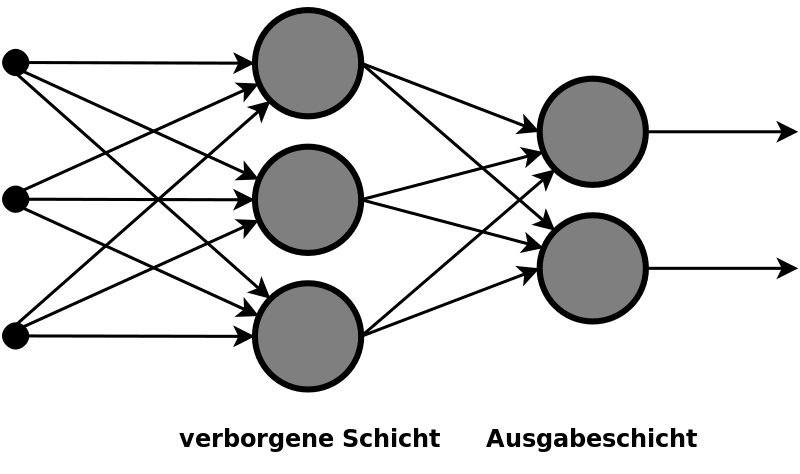
\includegraphics[totalheight=0.2\textheight]{Bilder/Multi-Layer_Neural_Network-Vector.png}
	\end{center}
	\caption{Zweischichtiges Netz (wiki)}
	\label{fig:Schichten}
\end{figure}
Ein jedes Neuron rechnet die hineinkommenden Eingabewerte mit einer zur Übertragungskante zugehörigen Gewichtung mit einer Übertragungsfunktion zusammen, die Anzahl der Eingaben ist hierbei unbegrenzt ("unlimited fan-in property" \cite{Rojas:1996:NNS:235222}). Die Übertragungsfunktion kann hierbei schlicht die Summe aller gewichteten Eingaben sein. Der errechnete Wert wird als Netzeingabe an die Aktivierungsfunktion gegeben. 
\\
\begin{figure}[h]
	\begin{center}
		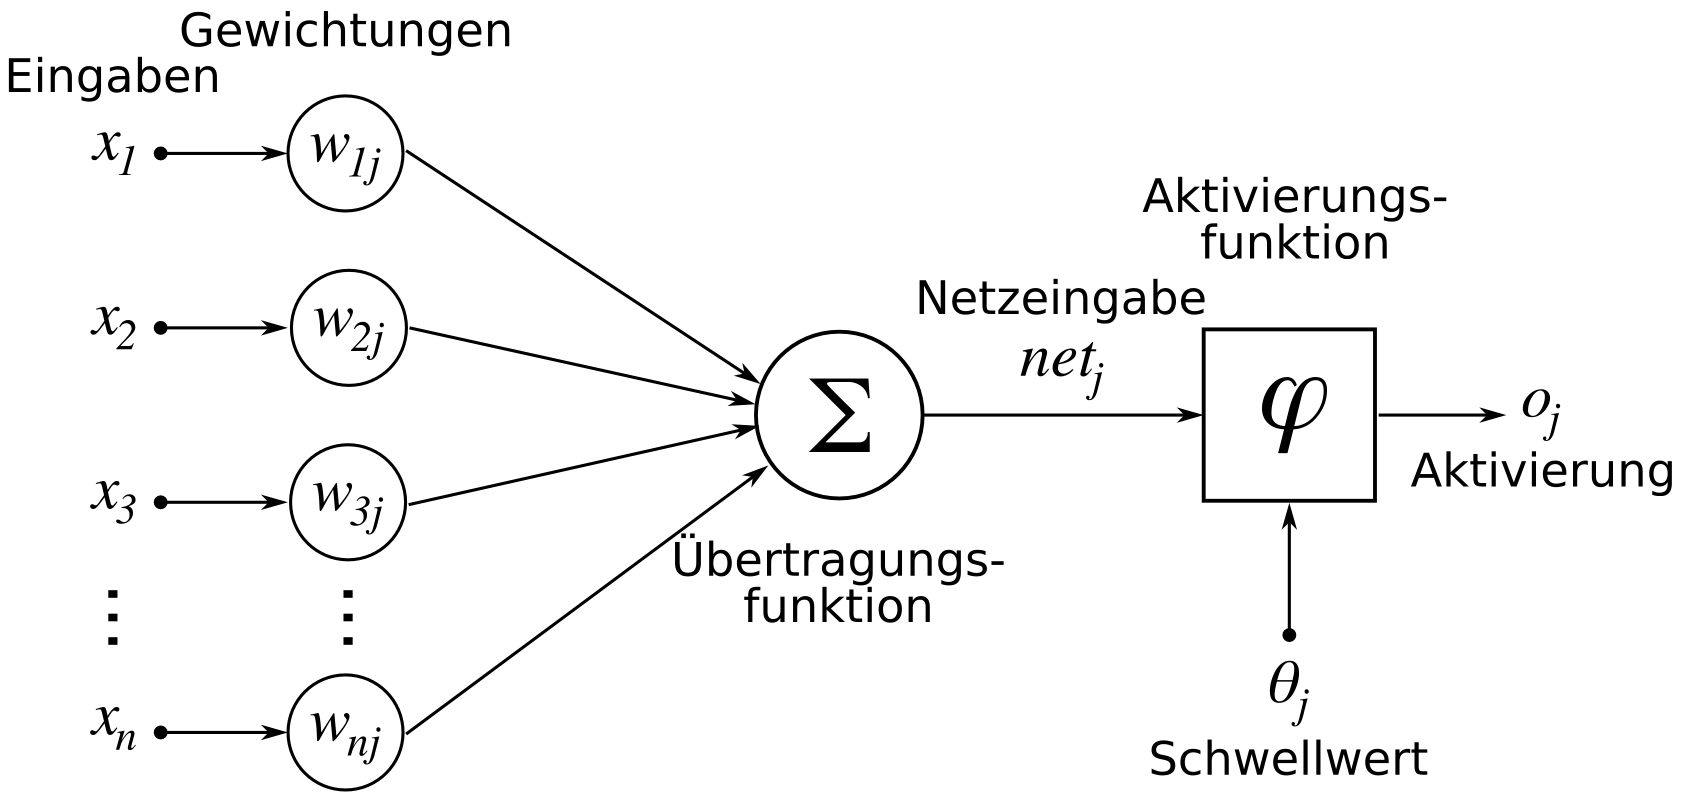
\includegraphics[totalheight=0.2\textheight]{Bilder/ArtificialNeuronModel_deutsch.png}
	\end{center}
	\caption{Schema eines künstlichen Neurons (wiki)}
	\label{fig:Neuron}
\end{figure} \\

Die Aktivierungsfunktion berechnet eventuell mit einem Schwellwert die Aktivierung des Neurons, welche dann an alle verbundenen Neuronen der nächsten Schicht gegeben wird. Die Aktivierungsfunktion kann beispielsweise eine simple Stufenfunktion sein, die allen Netzeingbaben kleiner des Schwellwertes eine Null und allen Eingaben größer gleich des Schwellwertes eine Eins zuweist.\\
Ein Neuron mit der gewichteten Summe aller Eingaben als Übertragungsfunktion und einer Stufenfunktion mit Schwellwert als Aktivierungsfunktion wird von Rojas Perzeptron bezeichnet \cite{Rojas:1996:NNS:235222} (Seite 60).
Ein feedforward-Netzwerk aus Perzeptrons, in dem jedes Neuron mit allen Neuronen der folgenden Schicht verbunden ist, wird als multilayer perceptron (kurz MLP) bezeichnet.
Ein neuronales Netz lernt die Abbildung zwischen den vorgegebenen Paaren von Eingabe- und Ausgabedaten durch Anpassung der Gewichte an den Kanten, nachdem es mit zufällig initialisierten Kantengewichten gestartet ist. Diese Anpassung geschieht beim MLP durch Fehlerrückführung (engl. backpropagation). Dabei wird der mittlere quadratische Fehler der berechneten Ausgabe gegenüber der vorgegebenen Ausgabe ermittelt und daraufhin unter Rücksichtnahme auf eine Lernrate mit Hilfe des Gradientenverfahren minimiert.
Vor der Anwendung eines künstlichen neuronalen Netzes für ein Problem stellt sich die Frage, ob dieses für das Problem geeignet ist. Dazu gibt es einige interessante mathematische Beweise.
Ein einzelnes Perzeptron kann alle linear separierbaren logischen Funktionen exakt approximieren \cite{Rojas:1996:NNS:235222} (Seite 62-63). 
Wobei lineare Separierbarkeit definiert ist als: Zwei Mengen von Pukten A und B .. (auf deutsch? ) \\

\begin{figure}[h]
	\begin{center}
		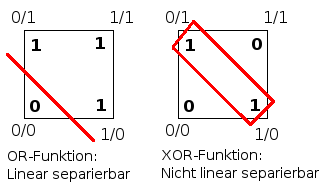
\includegraphics[totalheight=0.2\textheight]{Bilder/Lineare_Separierbarkeit.png}
	\end{center}
	\caption{Lineare Separierbarkeit von Funktionen (wiki)}
	\label{fig:Neuron}
\end{figure} 

Diese Beschränkung gilt allerdings nicht für ein Netzwerk von Neuronen. Bereits ein zweilagiges Netzwerk aus noch simpleren McCulloch-Pitts-Zellen kann jede beliebige logische Funktion berechnen \cite{Rojas:1996:NNS:235222} (Seite 37).
Für MLPs hat Cybenko \cite{cybenko:mcss} bewiesen, dass sie belieblige kontinuierliche Funktionen auf einer kompakten Teilmenge des euklidischen Raums $\mathbb{R}^n$ approximieren kann. Der entsprechende Satz hierzu ist das "universal approximation theorem".

\bigskip
\paragraph{Zusammenfassung:}
\textit{2-5 Sätze, BLA In diesem Kapitel hab ich gesehen BLA und jetzt sehen wir Z. Wie hängen die Sections dieses Kapitels zusammen und warum brachte es was das zu lesen.}


\chapter{Verwandte Arbeiten}
\textit{%
	Es finden sich keine wissenschaftlichen Veröffentlichungen die sich auch mit dem Einsatz von neuronalen Netzen zur Vorhersage von E/A-Leistung im Hochleisungsrechnen befassen. Jedoch werden die verschiedenen Teilgebiete des Themas behandelt. Um weniger Umschreiben zu müssen führe ich zunächst zwei Kategorien von Lösungsansätzen ein. Danach erwähne ich kurz einige Arbeiten, dessen Themen sich mit dem dieser Arbeit überschneiden, und danach gehe ich noch etwas detailierter auf Veröffentlichungen mit hoher Ähnlichkeit und Relevanz ein.
}
\bigskip

\section{Leistungsvorhersage von Ein-/Ausgabe}

\subsection{Kategorisierung}
	Das Problem, die Zugriffszeiten auf Festplatten vorherzusagen, kann im wesentlichen durch zwei verschiedene Ansätze gelöst werden.\\ Zum einen kann man versuchen das Festplattensystem in einem Modell nachzubilden, indem Hardwaredetails, wie die Rotationsgeschwindigkeit der Platte, die Reaktionszeit und Geschwindkeit des Lesekopfs, sowie das Zusammenspiel der Komponenten bekannt sind oder entsprechende Parameter durch gezielte Untersuchung approximiert werden. Mit diesem möglichst exakten Modell können dann Zugriffe simuliertd und die Laufzeit des Modells gemessen werden. Diese Messung kann daraufhin als Vorhersage für das reale System verwendet werden.\\
Der zweite Ansatz ist auch der dieser Arbeit, es wird von dem eigentlichen Festplattensystem abstrahiert und stattdessen ein mathematisches Modell gesucht,
das das Verhalten des Systems möglichst genau beschreibt. Zur Entwicklung des mathematischen Modells werden gemessene Leistungswerte von Festplattenzugriffen untersucht, um daraus passende Parameter für das Modell abzuleiten. Ich unterscheide daher im Folgenden zwischen dem Modellierungssansatz, bei dem versucht wird das Festplattensystem nachzubilden (in der englischen Fachliteratur auch als analytic device modeling bzw. simulation modeling bezeichnet) und dem Interpolationsansatz, bei dem ein numerisches Modell entwickelt wird. Da hier ohne Wissen über die inneren Zustände des Systems modelliert wird, wird dieser Ansatz auch black-box modeling bezeichnet. (\textbf{Quelle}? Fourier assisted ml)
	
\subsection{Modellierungssansatz gegenüber Regressionsansatz}
	Die Nachteile von Modellen mit Modellierungssansatz liegen insbesondere daran, dass sie aufwendig zu konfigurieren sind "In fact, one of us (Oldfield) spent several months configuring DiskSim to model an existing device" \cite{Crume:2013:FML:2538542.2538561} (S.1) und naturgemäß schnell veraltern, da sie jeweils an spezielle Hardware angepasst sind. Der Vorteil dagegen ist, dass sie bei korrekter Konfiguration sehr präzise sind, wie z.B. hier gezeigt \cite{Ruemmler94anintroduction}. \\
	Der Interpolationsansatz ist in der Anwendung einfacher und flexibler, da es sich automatisch an das System anpasst. Dafür erwartet man aufgrund der fehlenden analytischen Einsicht ins System eine etwas schlechtere Präzision. \\ Für die Anwendung im HPC-Bereich spielt der analytische Ansatz eine untergeordnete Rolle, da hier unterschiedliche Festplattensysteme zusammenarbeiten und stark mit der Netzwerkarchitektur verstrickt sind, sodass eine entsprechende Analyse des Systems zu aufwendig wird. "Furthermore, [...] building an accurate model or simulator using white box method cannot be a genereal solution in serving a variety of very different workloads" \cite{DBLP:conf/npc/ZhangLZJC10} (S.2, Zeile 20-24).\\
	
	Eine weitere Arbeit, in der ein Modellierungsansatz genutzt wird stammt von Lebrecht et al. \cite{Lebrecht:2009:10.1109/QEST.2009.31}.\\ 
	Bei Arbeiten, in denen ein Interpolationsansatz genutzt wird, werden verschiedene Data-Mining bzw. stochastischen Methoden angewandt, beispielsweise eine Kombination aus regression trees und support vector mashines  \cite{Dai:2012:SDP:2477169.2477214}, bagging classification und regression trees \cite{DBLP:conf/npc/ZhangLZJC10}. Verschiedene statistische Methoden werden von Kelly et al. untersucht \cite{Kelly04inducingmodels}.\\

\subsection{Fourier-Assisted Machine Learning}
Adam Crume et al. \cite{Crume:2013:FML:2538542.2538561} gehen davon aus, dass der entscheidende Faktor bei der Vorhersage von Zugriffszeiten in der Erkennung von periodischen Mustern liegt. Diese Annahme ist für eine einzelne Festplatte gerechtfertigt, da man die Zugriffstzeit grob in zwei Teile aufteilen kann, zum einen die Bewegung des Lesekopfs auf die richtige Spur und die Bewegung des Kopfes entlang der Spur zum richtigen Punkt, auch wenn diese beiden Bewegungen in der Realität überlappen. Jede Festplattenspur hat entsprechend des Radius eine andere Periodendauer.\\
Durch eine Fourier Analyse finden sie die Hauptfrequenzen heraus und können diese dann nutzen, um mit einem neuronalen Netz Vorhersagen zu treffen.
Eine Schwierigkeit in dieser Arbeit ist unter anderem, dass durch die große Anzahl Perioden nur ein kleiner Ausschnitt der Festplatte in seiner Gesamtheit, also alle möglichen Paare von Ausgangs- und Endspuren, untersucht werden kann. Die Priorität solcher Frequenzen für die exakte Leistungsvorhersage, ist im komplexen HPC-E/A-System zunächst einmal nicht zu erwarten, müsste allerdings untersucht werden.

\section{Leistungsvorhersage mit neuronalen Netzen}
Artificial neural networks for modelling and control of non-linear systems
\url{https://books.google.de/books?hl=de&lr=&id=tmTTBwAAQBAJ&oi=fnd&pg=PR9&dq=%22neural+networks%22+storage&ots=KyYA14xY1w&sig=yAQG0zn41xAHccDNaUWYd3L_ywI}


\section{Leistungsvorhersage im Hochleistungsrechnen}

	Im HPC Bereich ist die Leistungsanalyse generell ein wichtiger Punkt, so wird beispielsweise das Scheduling-Algorithmen vom Dateisystem simuliert \cite{Liu_towardssimulation}, hier wird DiskSim \cite{Bucy08thedisksim} zur Vorhersage der Festplattenzugriffszeiten genutzt, dabei nutzt DiskSim einen Modellierungssansatz (analytical simulation). \\

Viele Projekte verwenden Neuronale Netze für die Modellierung vom Gehirn....
http://world-comp.org/p2012/PDP3003.pdf

Machine Learning for Machines: Data-Driven Performance Tuning at Runtime Using Sparse Coding
SJ Tarsa - 2015 - dash.harvard.edu
... 83 5.2 Workload Models and Data Collection . . . . . 85 5.3 Predicting Storage
Performance with CART . . . . . 87 5.3.1 Applying CART to Multi-Tenant Scenarios . . . . .
87 5.3.2 Variation-Tolerant CART Using Workload Labels . . . . . ... 

Predicting disk drive failure at a central processing facility using an evolving disk drive failure prediction algorithm

ABER sie werden nur unzureichend eingesetzt für I/O und deswegen braucht es die Arbeit.

10-20 andere literatur

\subsection{Predicting Performance of Non-Contiguos I/O with Machine Learning}
Direkt aus dem Bereich des Hochleistungsrechnens stammt die Arbeit von Kunkel et. al \cite{UMLTPTPONI15}. Hier wird versucht mit Hilfe von decision trees die performantesten Parameter für nicht zusammenhängende Zugriffe auf Dateien durch ROMIO, einer Implementierung von MPI-2 I/O, zu finden. Dabei sagen sie mit den decision trees die Performance für die verschiedenen Parameter auf den Daten voraus, sodass sie anhand dieser Vorhersagen die besten Parameter finden. (\textbf{habe ich das richtig verstanden}?) Mit dieser Methode haben sie es geschafft zufriedenstellende Ergebnisse zu erzielen. Die Simplizität von decision trees, beispielsweise können diese nur Entscheidungen als eine Aneinanderreihung von linearen Separationen des Werteraums treffen, lässt vermuten, dass mit Hilfe von komplexeren Data Mining - Methoden, wie neuronalen Netzen noch bessere Ergebnisse erzielt werden könnten. Hier findet sich ein potenzielles Anwendungsgebiet der Ergebnisse dieser Bachelorarbeit.

\paragraph{Zusammenfassung:}
\textit{2-5 Sätze, BLA In diesem Kapitel hab ich gesehen BLA und jetzt sehen wir Z. Wie hängen die Sections dieses Kapitels zusammen und warum brachte es was das zu lesen.}


\chapter{Gestaltung der Analyse}
\textit{%
	Was wird warum und auf welche Weise gemacht? Konzepte aufschreiben
}
\bigskip

\section{Vorgehensweise}
** Daten exploriert\\



\section{Modell der Ein-/Ausgabe}
\label{ea_modell}
Um eine Idee dafür zu bekommen, wie die Modelle in etwa gestaltet sein müssen, die Zugriffszeiten abbilden zu können, wird hier zunächst ein grobes Modell der E/A aufgestellt.\\
Anhand der Verarbeitung eines Leseaufrufs gehe ich die Stufen des E/A-Systems durch. Wie in \ref{E/A} beschrieben hängt die Zugriffszeit davon ab, in welcher Speicherebene die angefragte Datei befindet. Für die Zugriffszeit kann im wesentlichen unterschieden werden, ob sich die angefragte Datei bereits innerhalb des anfragenden Rechnerknoten befindet oder diese von einer Festplatte außerhalb des Knotens geholt werden muss.
Falls die sich die Datei nicht im Speicher des Rechnerknotens befindet, muss als erstes eine Anfrage an das angebundene E/A-System gestellt werden. Der Verwaltungsaufwand der Anfrage sollte im wesentlichen für alle Aufrufe konstant sein, denn sie sieht strukturell für aufwendige Aufrufe nicht anders aus, als für weniger aufwendige.
Daraufhin muss das E/A-System die Festplatten ansprechen (evt. auch mehrere) auf der die gewünschte Datei liegt. Der Aufwand für den Aufbau der Verbindung zum Speicherort der Datei ist dabei stark von der Struktur des Netzwerkes abhängig. Die Festplatte liest die Datei aus und schickt sie über das Netzwerk an den Rechnerknoten auf dem sie benötigt wird.
Ebenso wie in dem Fall, in dem keine Anfrage außerhalb des Rechnerknotens gestellt werden musste, muss nun der erforderliche Teil der angefragen Datei noch aus dem Arbeitsspeicher des Knotens in den Cache des Prozessors geladen werden, auf dem der Prozess die Datei angefragt wurde. Für einen Schreibzugriff gilt im Wesentlichen ein ähnlicher Ablauf, der Datenfluss ist nur umgekehrt.\\
Es können also drei voneinander unabhängige Anteile der Zugriffszeit unterschieden werden. Die Zeit, die für die Verwaltung der E/A-Anfrage und die Dateiübertragung über das Netzwerk benötigt wird (tNetzwerk), sowie für die Verarbeitung auf der Festplatte (tHDD) und für das Lesen/Schreiben von dem Arbeitsspeicher (tMem).\\
In allen Bereichen gibt es jeweils einen konstanten Anteil und einen Anteil, der von der aufgerufenen Datei abhängt. 
Der Anteil der Zugriffszeit, die für jeden Aufruf konstant ist, ist für die Modellierung weniger spannend und sollte bereits durch einfache linerare Modelle darstellbar sein, dieser Teil wird im Folgenden nicht weiter berücksichtigt.

Der Netzwerkabhängige Teil ist zum einen von der genauen Lokalität der aufgerufenen Datei, sowie der größe der Datei abhängig. Der Datenfluss über das Netzwerk hängt von dessem Durchsatz ab, dieser sollte nach kurzer Verbindungsaufbauphase konstant sein. Im Rahmen meiner Instrumentierungsmöglichkeiten ist es nicht möglich die Abhängigkeit der Zugriffszeit von Speicherort im Netzwerk direkt vorherzusagen. Dazu wäre ein Einblick in eine Datenbank notwendig, aus der sich solche Informationen ableiten ließen, oder eine solche Wissensbasis müsste selbst aufgebaut werden. \textbf{(allerdings greifen wir ja eh immer auf die gleiche Datei zu, sodass das Netzwerk keine Rolle spiel?)}
tMem ist am einfachsten zu modellieren, denn der Direktzugriffsspeicher (engl. Random-Access Memory) kennzeichnet sich gerade dadurch, dass der Zugriff auf alle Datenblöcke mit geichem Aufwand verbunden ist. Ansonsten hängt die Zugriffszeit vom Durchsatz des Speichers ab, der auch linear von Größe des angefragten Dateibereichs abhängt.
Die Festplatte ist ähnlich Komplex wie das Netzwerk, kann allerdings im Rahmen der durchgeführten Testläufe näher untersucht werden, indem immer wieder auf der selben Platte gearbeitet wird. Wie beim Netzwerk ist die Zugriffszeit zum einen von dem genauen Ort der angefragten Datenblöcke und zum anderen vom Durchsatz der Festplatte abhängig. Die Abhängigkeit vom Ort schlägt sich in dem Abstand des Aufenthaltsortes des Lesekopfes vor dem Aufruf zu dem Zielort auf der Festplatte nieder, im Folgenden wird dieser Abstand als Delta-Abstand bezeichnet. Der zeitliche Aufwand des Überwinden des Delta-Abstandes ist Hardwarecharakteristika der Festplatte abhängig. Zum einen die Zeit, die der Lesekopf benötigt, um von der aktuellen Festplatten-Spur zur Zielspur zu kommen und zum anderen, die Rotationszeit der Magnetscheibe, die den Lesekopf in der Horizontalen zur richtigen Stelle befördert. Dabei geschehen Spurwechsel und Rotation auch gleichzeitig. Ansonsten ist die Zugriffszeit linear von dem Durchsatz der Festplatte und der Größe des angefragen Abschnittes abhängig.

Während also tMem vollständig lineares Modell dargstellt werden können müsste, ist dies für tNetzwerk und tHDD nur bedingt der Fall. Netzwerk und Festplatte haben einen bestimmenden linearen Anteil, jedoch auch einen Speicherort abhängigen.
Die Durchsätze von tMem, sowie tHDD sind Hardware bedingt von der Art des Zugriffs abhängig, es muss also zwischen Lese- und Schreibzugriffen unterschieden werden, dies ist im Folgenden der Operationstyp (OpTyp).
Das Modell für die Ein-/Ausgabe in dieser Arbeit entspricht letztendlich

\begin{align*}
&tGesamt = tNetzwerk + tMem + tHDD\\
&\text{mit}\\
&tNetzwerk(Grö\text{ß}e, Netzwerkspeicherort)\\
&tMem(Grö\text{ß}e,OpTyp)\\
&tHDD(Grö\text{ß}e,OpTyp,Delta\text{-}Abstand)\\
\end{align*}

Die Vermutung in dieser Arbeit ist, dass sich E/A-Aufrufe in verschiedene Pfade unterteilen lassen, dabei entspricht der Pfad der Verbindung vom aufrufenden Prozess zur aufgerufenen Datei. Ein perfektes Modell könnte unter Kenntnis dieses Pfades und der Dateiattribute die Dauer des Zugriffs exakt vorhersagen.\\
Im Benchmark-Test (\ref{benchmark}) wird zu jeder gemessenen E/A-Prozedur die Größe des gelesenen/geschriebenen Bereichs, der Operationstyp und der Delta-Abstand gemessen.
Das Tripel $(Grö\text{ß}e,OpTyp,Delta-Abstand)$ bezeichne ich als Attribut-Set der Messung.

\section{Leistungs- und Ausreißervorhersage}
Mit den im Weiteren entwickelten Modellen soll untersucht werden, wie gut es gelingt den Aufwand der E/A-Aufrufe vorherzusagen. 
Die im Benchmark-Test gemachten Messungen werden dabei genutzt. Zunächst kann das Modell einen Teil der Daten zum Lernen nutzen und dann können die Vorhersagen des Modells zu ungesehenen Messungen mit den tatsächlichen Werten verglichen werden. Dies ist die Leistungsvorhersage vom Modell zum System. 
Desweiteren wird die Ausreißervorhersage des Modells betrachtet werden. Als Ausreißer werden dabei die Messungen bezeichnet, die eine ungewöhnlich schnelle oder langsame Laufzeit haben. Es handelt sich hierbei in diesem Kontext nicht um invalide Messungen, für die die Instrumentierung des Experiments verantwortlich ist, denn es wird schlicht intern die Zeit von Anfang bis Ende eines E/A-Aufrufs gemessen. Stattdessen kann es beispielsweiese sein, dass das System punktuell sehr ausgelastet war. 
Bei der Ausreißervorhersage wird geprüft, ob das Modell korrekt voraussagen kann, dass die Laufzeit einer E/A-Anfrage zu den Ausreißern gehört. Da es sich bei den Ausreißern nicht um Messfehler handelt ist eine solche Vorhersage prinzipiell möglich, erfordert allerdings eine sehr gute Einsicht ins System.
Man könnte die Ausreißervorhersage auch als Test auf den schwierigsten Daten ansehen. Es würde für die Qualität eines Modells sprechen, wenn es sowohl eine gute Leistungsvorhersage, auch eine gute Ausreißervorhersage macht. Da die Informationen, die den Modellen zur Verfügung stehen allerdings nicht für eine verlässliche Ausreißervorhersage ausreichen sollten (beispielsweise wäre dazu Wissen über parallel laufende Prozesse unter anderem von anderen Benutzern des Hochleistungsrechners notwendig), könnte dieser Test auch ein Maß für eine zu starke Adaption an die Trainingsdaten sein.


\section{Modellklassen}
Modelle unterscheiden sich an den Informationen, die Ihnen über die Messdaten zur Verfügung stehen.\\

Da es sich bei der E/A-Leistungsvorhersage um ein komplexes Problem handelt, steht nicht a priori fest, wie eine passende Modellierung auszusehen hat. 
In dieser Arbeit wurden daher verschiedene Ansätze getestet. Um besser zu verstehen, welche Ideen einem Modell zugrunde liegen und zur einfacheren Beschreibung der Modelle führe ich verschiedene Kategorien von Modellen ein die jeweils einem bestimmten Ansatz entsprechen.
Die Modellklassen unterscheiden sich in ihrer Herangehensweise ans Problem. Modelle, die den selben Klassen zugehören, unterscheiden sich an den Informationen, die ihnen über die Messdaten zur Verfügung stehen.

\subsection{Triviale und höhere Modelle}
Triviale Modelle werden auf einfache Weise mit klassischen mathematischen Methoden mit relativ geringem Rechenaufwand berechnet. Die höheren Modelle in dieser Arbeit basieren dagegen auf neuronalen Netzen und müssen aufwendig trainiert werden.\\
Die trivialen Modelle sind zum einen beim Erkunden sinnvoller Ansätze hilfreich, zum anderen dienen sie dem Vergleich der aufwendigeren Modelle und stellen eine untere Schranke für deren Leistungen dar. So kann an den Ergebnissen eines Modells, das bloß lineare Zusammenhänge beschreiben kann, untersucht werden, ob die Daten in linearer Weise beschrieben werden können. Die Erwartung ist, dass die höheren Modelle wesentlich bessere Ergebnisse zeigen, als die trivialen. Wenn dies nicht der Fall ist, war entweder die Modellierung schlecht oder die zur Verfügung stehenden Messdaten sind unzureichend für eine zufriedenstellende Beschreibung.
Eine Ausnahme bilden dabei unfaire triviale Modelle, die mit Informationen ausgestattet sind, die sie als legitimes Modell nicht haben dürften. Beispielsweise sind dies Modelle, die Testdaten bereits kennen. Diese Modelle dienen zur Überprüfung, was mit einem Konzept maximal machbar ist.

\subsection{Zeitreihen- und Aggregierungs-Modelle}
Für Aggregierungsmodelle werden die Trainingsdaten stark vereinfacht. Sie verfolgen den Ansatz, dass es nicht möglich ist innerhalb eines Attribut-Sets zu differenzieren. Sodass verschiedene Messungen eines Sets alle die selbe Vorhersage zugewiesen bekommen. Dazu werden alle Trainingsdatenpunkte zusammengefasst, die zum selben Set gehören.

Bei Zeitreihen-Modellen hingegen findet keine Aggregierung statt. Zu verschiedenen Messungen eines Attribut-Sets gibt es entsprechend \glqq widersprüchliche\grqq{} Informationen, da sich ihre Laufzeit unterscheidet. Das Modell muss dann entweder intern die Daten zusammenfassen, um doch die selbe Vorhersage für jede Messung eines Sets zu machen oder es versucht anhand weiterer Informationen über den Systemzustand eine Differenzierung durchzuführen. Dieses zusätzliche Wissen über den aktuellen Zustand des Systems kann allerdings nur über die Kenntnis der vorherigen E/A-Aufrufe abgeleitet werden, denn die in \ref{ea_modell} beschriebenen Attribute bleiben die einzigen Informationen, die zu einer Messung zur Verfügung gestellt werden.
Die Zeitreihen-Modelle können also versuchen ein periodisches Systemverhalten zu erkennen und dieses für ihre Vorhersage auszunutzen. So könnte es beispielsweise sein, dass jeder dritte Leseaufruf doppelt so lange, wie die vorherigen dauert, weil das E/A-System zunächst einem anderen Prozess Priorität gibt, wenn dieses Verhalten erkannt wird, könnte die Vorhersage erheblich verbessert werden.

\subsection{Fehlerklassen-Modelle}
Um die These zu untersuchen, dass sich E/A-Aufrufe im System mit unterschiedlichen Pfaden ausdrücken lassen und die verbesserten Vorhersagen zu untersuchen, die unter Kenntnis dieser Pfade gemacht werden können, werden Modelle mit der Zusatzinformation von Fehlerklassen (FK) analysiert.
Fehlerklassen werden mit Hilfe der Vorhersagen eines anderen Modells berechnet. Der Fehler der Vorhersagen gegenüber den tatsächlichen Laufzeiten der E/A-Aufrufe wird mit dem k-Means-Algorithmus (\ref{ML}) in Cluster unterteilt. Jede Cluster-Gruppe entspricht einer Klasse und bekommt eine Nummer. 
Die Klassen repräsentieren unterschiedliche Pfade, die im E/A-System genommen wurden. (\textbf{WARUM?})
Wenn das Modell, das zur Generierung der Fehlerklassen genutzt wurde, und das Modell, das mit Wissen über diese Fehlerklassen, neue Vorhersagen macht ähnlich funktionieren, sollten die Ergebnisse dadurch wesentlich besser werden. Das liegt daran, dass das Modell bereits \glqq weiß\grqq{}, welchen Fehler es bei einer Vorhersage ohne Berücksichtigung der Fehlerklasse machen würde. 

\section{Untersuchte Modelle}
\label{impl:modelle}
Agregierungsmodelle haben (unfaire -> aber ok, da nur für baselines) globale Sicht\\

Ich stelle kurz alle Modelle vor, die untersucht wurden. Zunächst gehe ich die trivialen Modelle durch, dann die höheren.

Das einfachste Modell ist \textit{Durchschnitt}, das Modell kennt den globalen arithmetischen Mittelwert aller gemessen Messungen und ist in sofern unfair. Da das Modell überhaupt nicht auf die Attribute der betrachteten Messungen eingeht, sollten alle anderen Modelle bessere Leistungen erbringen. Einem Modell, das diese Informationen ausnutzt, mit schlechterer Leistung könnte unterstellt werden zufällige Vorhersagen zu machen und man kann auf eine Fehlfunktion schließen.

Eine ähnliche Methode verwendet das Modell \textit{Median agg}. Dies ist auch ein unfaires Modell, dass Kenntnis über alle Messungen in den Datensätzen hat. Es berechnet für jedes Attribut-Set den Median der Laufzeiten, dieser Wert entspricht dann der Vorhersage des Modells für Messungen dieses Sets. Dieses Modell stimmt mit dem Ansatz überein, eine Datenbank aufzubauen, in der alle E/A-Aufrufe und deren Laufzeiten gespeichert werden würden. Diese triviale Variante ist der Idealfall dazu, bei dem es zu allen auftretenden Attribut-Sets bereits einen gespeicherten Mittelwert gibt.

Während die ersten beiden Modelle Aggregations-Modelle sind, sind die Modelle, denen lineare Regression zugrunde liegt Zeitreihen-Modelle.
Lineare Regression ist ein einfaches numerisches Verfahren, dass eine lineare Funktion berechnet, die den Fehler zu den bekannten Messpunkten minimiert. Die Funktion ist eine Gerade der Form $f(x) = a + b*x$, mit der Verschiebung a und Steigung b. Wird die Regression über mehrere Variablen gemacht erhält man Verschiebungen und Steigungen, die sich aus den Komponenten zu jeder Variable zusammensetzen.
Ich probiere drei verschiedene lineare Modelle aus.
\textit{LinReg G} wird nur aus dem Zusammenhang von Zugriffsgröße und Laufzeit berechnet.
\textit{LinReg GA} enthält auch die Werte zu Delta-Abstand und \textit{LinReg GAO} berücksichtigt zudem den Operationstyp der Messungen.
Die Modelle können wegen der linearen Form nicht innerhalb eines Attribut-Sets unterscheiden. Sollte das vermessene E/A-System bereits durch lineare Zusammenhänge in den gemessenen Informationen beschreibbar sein, so sollten diese Modelle gute Ergebnisse zeigen.

Zuletzt gibt es noch zwei weitere Aggregations-Modelle, die Fehlerklassen ausnutzen.
Sie funktionieren genauso, wie \textit{Median agg}, nur das sie Messungen zusätzlich noch durch ihre Fehlerklasse unterscheiden. Es wird also der Median für jedes Attribut-Set berechnet, die zur selben Fehlerklasse gehören.
\textit{Median agg LinReg-FK} kennt die Fehlerklassen, die aus der Clusteranalyse der Fehler von \textit{LinReg G} gewonnen worden, und \textit{Median agg Tupel1-FK} die Klassen der besten Instanz von \textit{Tupel1}.

Das Aggregations-Modell \textit{Tupel1 agg} entspricht der fairen Variante zu \textit{Median agg}, das Modell kennt, so wie alle höheren Modelle, nur einen Ausschnitt der Messdaten, dies sind seine Trainingsdaten. Im Gegensatz zum zuvor betrachteten Idealfall muss das Modell die Laufzeiten unbekannter Mess-Attribute interpolieren. Das neuronale Netz des Modells bekommt als Eingabedaten alle Attribut-Sets mit aggregierten Laufzeiten aus seinen Trainingsdaten. Das Netz lernt dann das Tripel $(Zugriffsgr\text{ß}e, Delta\text{-}Abstand, Operationstyp)$ in Relation zum zugehörigen Median der Laufzeiten zu bringen.
Das Modell muss sich nicht bloß die Laufzeiten zu den Attribut-Sets \textit{merken}, sondern möglichst gut die Zusammenhänge zwischen den Attribut-Werten und den zugehörigen Laufzeit-Mediane bestimmen, um unbekannte Attribut-Sets sinnvoll vorhersagen zu können.

Ähnlich dazu agiert das Modell Zeitreihen-Modell \textit{Tupel1}. Die Eingabedaten werden allerdings nicht aggregiert. Es versucht also direkt das beschriebene Tripel auf die zugehörigen Laufzeiten abzubilden. Es hat sonst keine weiteren Informationen, sodass es ebenso wenig, wie das Aggregationsmodell, zwischen Messungen mit gleichen Attributen unterscheiden kann.

\textit{Tupel2} bekommt nicht nur die Attribute der Messung, dessen Leistung es vorhersagen soll, sondern auch die Attribute und die Laufzeit der vorherigen Messung. Die Idee hierbei ist, dass anhand des Wissens, wie schnell die letzte E/A-Prozedur bearbeitet werden konnte, eine Aussage über die Nächste getroffen werden kann. Falls das System beispielsweise gerade besonders ausgelastet ist, würde sich dies an der vergangenen E/A-Leistung niederschlagen. Es könnte auch sein, dass das System eine sehr simple Periodizität aufweist. Sodass, nach einer schnellen Bearbeitung eine langsame folgt oder Ähnliches.

Eine tieferliegende Periodizität könnte unter Umständen durch \textit{Tupel1 gleitender Durchsatz} ausgenutzt werden.

\subsection{Attribut Selektion und Generierung}
Korrelationen untersuchen, neues Attribute generieren (wesentlich für die verschiedenen Modelle)\\

jedes Modell beschreiben\\
welche Attribute hat das Modell\\
jeweils Beschreiben, wie die Daten hierfür vorbereitet werden mussten\\
was die Idee davon ist\\
warum macht es Sinn, dies zu testen\\

\section{Anwendung und Parameter}
Wie werden die richtigen Parameter für jedes Modell gefunden? -> Systematisches Testen der Parameter
Wie wird mit Ausreißern umgegangen, wie werden sie definiert\\
Aufteilung der Daten in Lern-und Testdatensatz, Cross-Validation; 40.000 Punkte von 400.000\\ 
-- *** Lernen von Read \& Write zusammen oder getrennt\\

Anzahl berechneter Netze pro Modell, threshold, Größe der Netze, lern- und fehler-funktionen\\


Alle Modelle haben einen Trainingsdatensatz, sowie einen Testdatensatz von Messungen 

\section{Validierung der Modelle}
*** Sampling der Datenmenge\\
Welche Leistungsmerkmale werden warum untersucht?\\
*** Welche Fehlermetriken verwenden wir?\\
mathematische Definitionen der metriken\\
**** Relativen Fehler, |Abs Fehler|, Summary von residuals summary(mess - pred), Summary (relative)\\
*** Ensemble Lernen\\
Zudem Vergleich mit durchschnittlicher Leistung von Netzen mit gleihen Parametern\\
- abhängigkeit von auswahl der trainingsdaten und lokaler konvergenz\\
Konzept und Anwendung, was soll damit erreicht werden? -> lin abh der netze\\


\section{Aufbau der Benchmark-Tests}
\label{benchmark}
Das Testsystem (\ref{impl:testsystem}) muss durch Vermessung von Experimenten untersucht werden. Mit Hilfe der Messdaten können die vorgestellten Modelle aus \ref{impl:modelle} entwickelt und anschließend getestet werden. Um die Stärken und Schwächen der Modelle gut untersuchen zu können, wird eine systematischer Ansatz für die Experimente gewählt. Die Aufzeichnung der Experimente geschieht durch SIOX \cite{UMLTPTPONI15}. Es wurden vier verschiedene Experimente gemessen, sie repräsentieren zwei unterschiedliche Anwendungsfälle. Die sich ergebenden Datensätze bezeichne ich als cached-off0-seq-R, cached-off0-seq-W, sowie cached-off0-rnd-R und cached-off0-rnd-W.\\
Bei allen Tests wurde die Datei, auf die sich die E/A-Anfragen beziehen, zunächst einmal eingelesen. Daher der erste Teil der Bezeichnung. Das genutzte Speicherlayout ist ein simples off0-Layout, das bedeutet, dass die gelesenen Daten an Position 0 des Arbeitsspeichers geschrieben werden, bzw. Informationen zum Schreiben immer von dort geholt werden. (\textbf{Stimmt das?})
Die Unterscheidung der beiden Anwendungsfälle (seq und rnd) befindet sich im Dateilayout. Während bei den cached-off0-seq Fällen ein sequentielles Layout der Datei gewählt wurde, sind diese bei cached-off0-rnd randomisiert. Beim sequentiellen Layout werden die E/A-Operationen jeweils hintereinander auf der Datei ausgeführt. Beispielsweise liest der erste Aufruf die ersten 10KB, der nächste die darauf folgenden 10KB. Dagegen wird beim randomisierten Layout auf einee beliebige Position der Datei zugegriffen. Das R steht für Read, also lesende Dateizugriffe und das W für Write, also schreibende Zugriffe.\\
Die Zugriffsgrößen variieren von 1KB bis 16MiB. E/A-Aufrufe werden mit einer festen Anzahl an Wiederholungen hintereinader mit der gleichen Zugriffsgröße durchgeführt (\textbf{Wie Oft?}). Die Testdatei ist 10GiB groß. Unter der Bezeichnung cached-off0-seq ist die Hintereinanderkettung der beiden Datensätze cached-off0-seq-R und cached-off0-seq-W zu verstehen. Gleiches gilt für cached-off0-rnd. 

\paragraph{Zusammenfassung:}
\textit{2-5 Sätze, BLA In diesem Kapitel hab ich gesehen BLA und jetzt sehen wir Z. Wie hängen die Sections dieses Kapitels zusammen und warum brachte es was das zu lesen.}\\


\chapter{Implementierung}
\textit{%
	Details: wie ist die Analyse tatsächlich umgesetzt?
}
\bigskip

\section{Verwendete Programmiersprache und Bibliotheken}
R,neuralnet etc.

\section{Modell-Parameter}
 systematisch erkundet

\section{Testsystem, Mistral}
\label{impl:testsystem}
Speziell die Hardware von Mistral, von hier kommen die Benchmarks\\

Als Testsystem für alle Messungen, die in dieser Arbeit untersucht werden, wurde der Hochleistungsrechner Mistral vom Deutschen Klimarechenzentrum (DKRZ) genutzt. Mistral befindet sich in der derzeit aktuellen Version vom Juni 2015 auf Platz 56 der von der TOP500-Organisation geführten Liste der schnellsten Supercomputer der Welt. Das System besteht aus über 1500 Knoten, die jeweils mit zwei Intel E5-2680v3 bestückt sind, diese laufen mit einer Taktfrequenz von 2.5GHz und haben jeweils 30MiB L3 Cache. Das Speichersystem des Rechners läuft mit dem parallelen und verteilten Dateisystem Lustre. Es bietet 30 Petabyte Speicherkapazität und eine Speicherbandbreite von 300 GiB/s. Die Messungen wurden während einer üblichen Belastungssituation des Systems durchgeführt, sodass Schwankungen in der Nutzung des E/A-Systems durch andere Nutzer die Messungen beeinflusst haben können.


\paragraph{Zusammenfassung:}
\textit{2-5 Sätze, BLA In diesem Kapitel hab ich gesehen BLA und jetzt sehen wir Z. Wie hängen die Sections dieses Kapitels zusammen und warum brachte es was das zu lesen.}

\chapter{Evaluierung}
\textit{%
	test
}
\bigskip

\section{Exploration der Daten}
Zunächst werde ich die vier Datensätze genauer betrachten. Dazu eignet es sich einige Metainformationen zu sammeln. In der Tabelle \ref{tab:meta} sind für alle vier Datensätze jeweils für die drei Attribute Dauer, Größe und Delta-Abstand der minimale Wert, der Wert des ersten Quartils, der Median, das arithmetische Mittel, der Wert des dritten Quartils, der maximale Wert und die Korrelation zu Dauer. Alle Datensätze bestehen aus 200.000 Messungen.\\

\begin{table}
	\scriptsize
	\subfloat[cached-off0-seq-R]{
		\begin{tabular}{|r|r|r|r|r|r|r|r|}\hline%
			Attribut & Min.  & 1. Quartil & Median & Arith. Mittel & 3. Quartil & Max. & Korrelation \\\hline\hline
			\csvreader[late after line=\\\hline]%
			{CSV/exploration/data_summary_read_seq.csv}{Attribut=\Attribut,Min=\Min,Quartil1=\L, Median = \Median, Mittel = \Mittel,Quartil3 = \Q, Max = \Max, Korrelation = \Korrelation}%
			{\Attribut & \Min & \L & \Median & \Mittel & \Q & \Max &\Korrelation}%
		\end{tabular}
	}\\
	\subfloat[cached-off0-seq-W]{
		\begin{tabular}{|r|r|r|r|r|r|r|r|}\hline%
			Attribut & Min.  & 1. Quartil & Median & Arith. Mittel & 3. Quartil & Max. & Korrelation \\\hline\hline
			\csvreader[late after line=\\\hline]%
			{CSV/exploration/data_summary_write_seq.csv}{Attribut=\Attribut,Min=\Min,Quartil1=\L, Median = \Median, Mittel = \Mittel,Quartil3 = \Q, Max = \Max, Korrelation = \Korrelation}%
			{\Attribut & \Min & \L & \Median & \Mittel & \Q & \Max &\Korrelation}%
		\end{tabular}
	}\\
	\subfloat[cached-off0-rnd-R]{
		\begin{tabular}{|r|r|r|r|r|r|r|r|}\hline%
			Attribut & Min.  & 1. Quartil & Median & Arith. Mittel & 3. Quartil & Max. & Korrelation \\\hline\hline
			\csvreader[late after line=\\\hline]%
			{CSV/exploration/data_summary_read_rnd.csv}{Attribut=\Attribut,Min=\Min,Quartil1=\L, Median = \Median, Mittel = \Mittel,Quartil3 = \Q, Max = \Max, Korrelation = \Korrelation}%
			{\Attribut & \Min & \L & \Median & \Mittel & \Q & \Max &\Korrelation}%
		\end{tabular}
	}\\
	\subfloat[cached-off0-rnd-W]{
		\begin{tabular}{|r|r|r|r|r|r|r|r|}\hline%
			Attribut & Min.  & 1. Quartil & Median & Arith. Mittel & 3. Quartil & Max. & Korrelation \\\hline\hline
			\csvreader[late after line=\\\hline]%
			{CSV/exploration/data_summary_write_rnd.csv}{Attribut=\Attribut,Min=\Min,Quartil1=\L, Median = \Median, Mittel = \Mittel,Quartil3 = \Q, Max = \Max, Korrelation = \Korrelation}%
			{\Attribut & \Min & \L & \Median & \Mittel & \Q & \Max &\Korrelation}%
		\end{tabular}
	}
	\caption{Metainformationen über die Datensätze}
	\label{tab:meta}
\end{table}

Das Attribut OpTyp kann nur sinnvoll über der Vereinigung von cached-off0-seq-R und cached-off0-seq-W bzw. cached-off0-rnd-R und cached-off0-rnd-W betrachtet werden. \ref{tab:metaoptyp}

\begin{table}
	\scriptsize
	\subfloat[cached-off0-seq]{
		\begin{tabular}{|r|r|r|r|r|r|r|r|}\hline%
			Attribut & Min.  & 1. Quartil & Median & Arith. Mittel & 3. Quartil & Max. & Korrelation \\\hline\hline
			\csvreader[late after line=\\\hline]%
			{CSV/exploration/data_summary_seq_optyp.csv}{Attribut=\Attribut,Min=\Min,Quartil1=\L, Median = \Median, Mittel = \Mittel,Quartil3 = \Q, Max = \Max, Korrelation = \Korrelation}%
			{\Attribut & \Min & \L & \Median & \Mittel & \Q & \Max &\Korrelation}%
		\end{tabular}
	} \\
	\subfloat[cached-off0-rnd]{
		\begin{tabular}{|r|r|r|r|r|r|r|r|}\hline%
			Attribut & Min.  & 1. Quartil & Median & Arith. Mittel & 3. Quartil & Max. & Korrelation \\\hline\hline
			\csvreader[late after line=\\\hline]%
			{CSV/exploration/data_summary_rnd_optyp.csv}{Attribut=\Attribut,Min=\Min,Quartil1=\L, Median = \Median, Mittel = \Mittel,Quartil3 = \Q, Max = \Max, Korrelation = \Korrelation}%
			{\Attribut & \Min & \L & \Median & \Mittel & \Q & \Max &\Korrelation}%
		\end{tabular}
	}
	\caption{Metainformationen über OpTyp, 1 entspricht einerm Leseaufruf und 2 einem Schreibaufruf}
	\label{tab:metaoptyp}
\end{table}


Nachdem nun ein grobes Verständnis für die vorliegenden Daten erlangt worden ist, folgt eine Betrachtung der tatsächlichen Messungen in Zeitreihe (\ref{Laufzeiten_Zeitreihe}). Um den wesentlichen Teil der Punkte besser erkennen zu können, wurden in den Graphen die obersten 1\%, also die langsamsten Datenpunkte, abgeschnitten.

\begin{figure}
	\subfloat{
		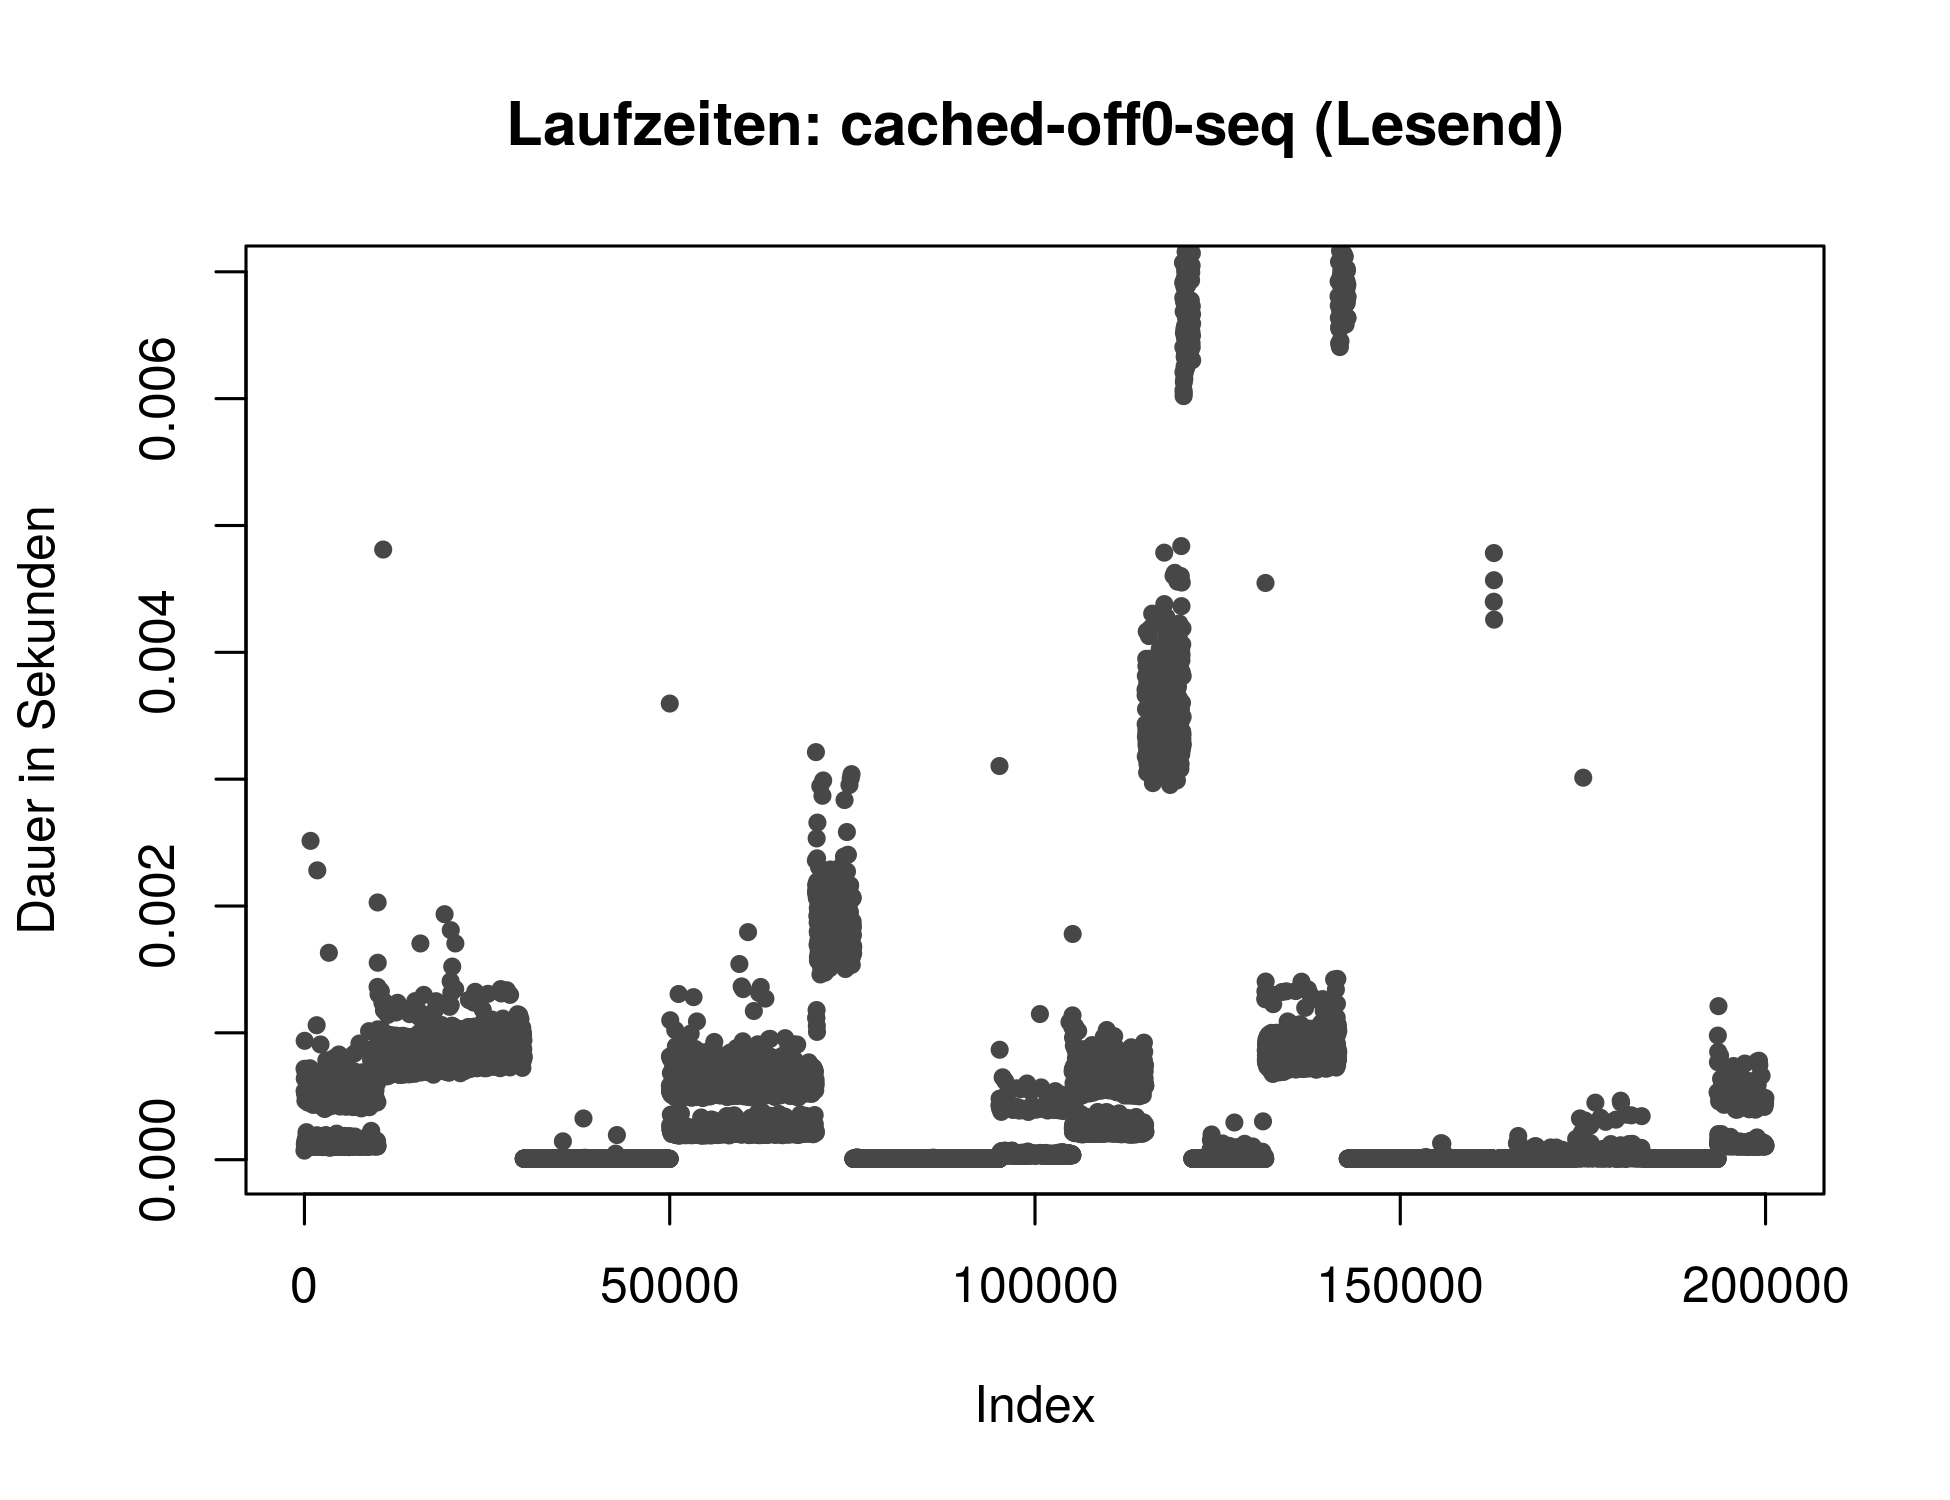
\includegraphics[width=.43\textwidth]{Bilder/Plots/exploration/plot_Duration_read_seq.png}
	}
	\hfill
	\subfloat{
		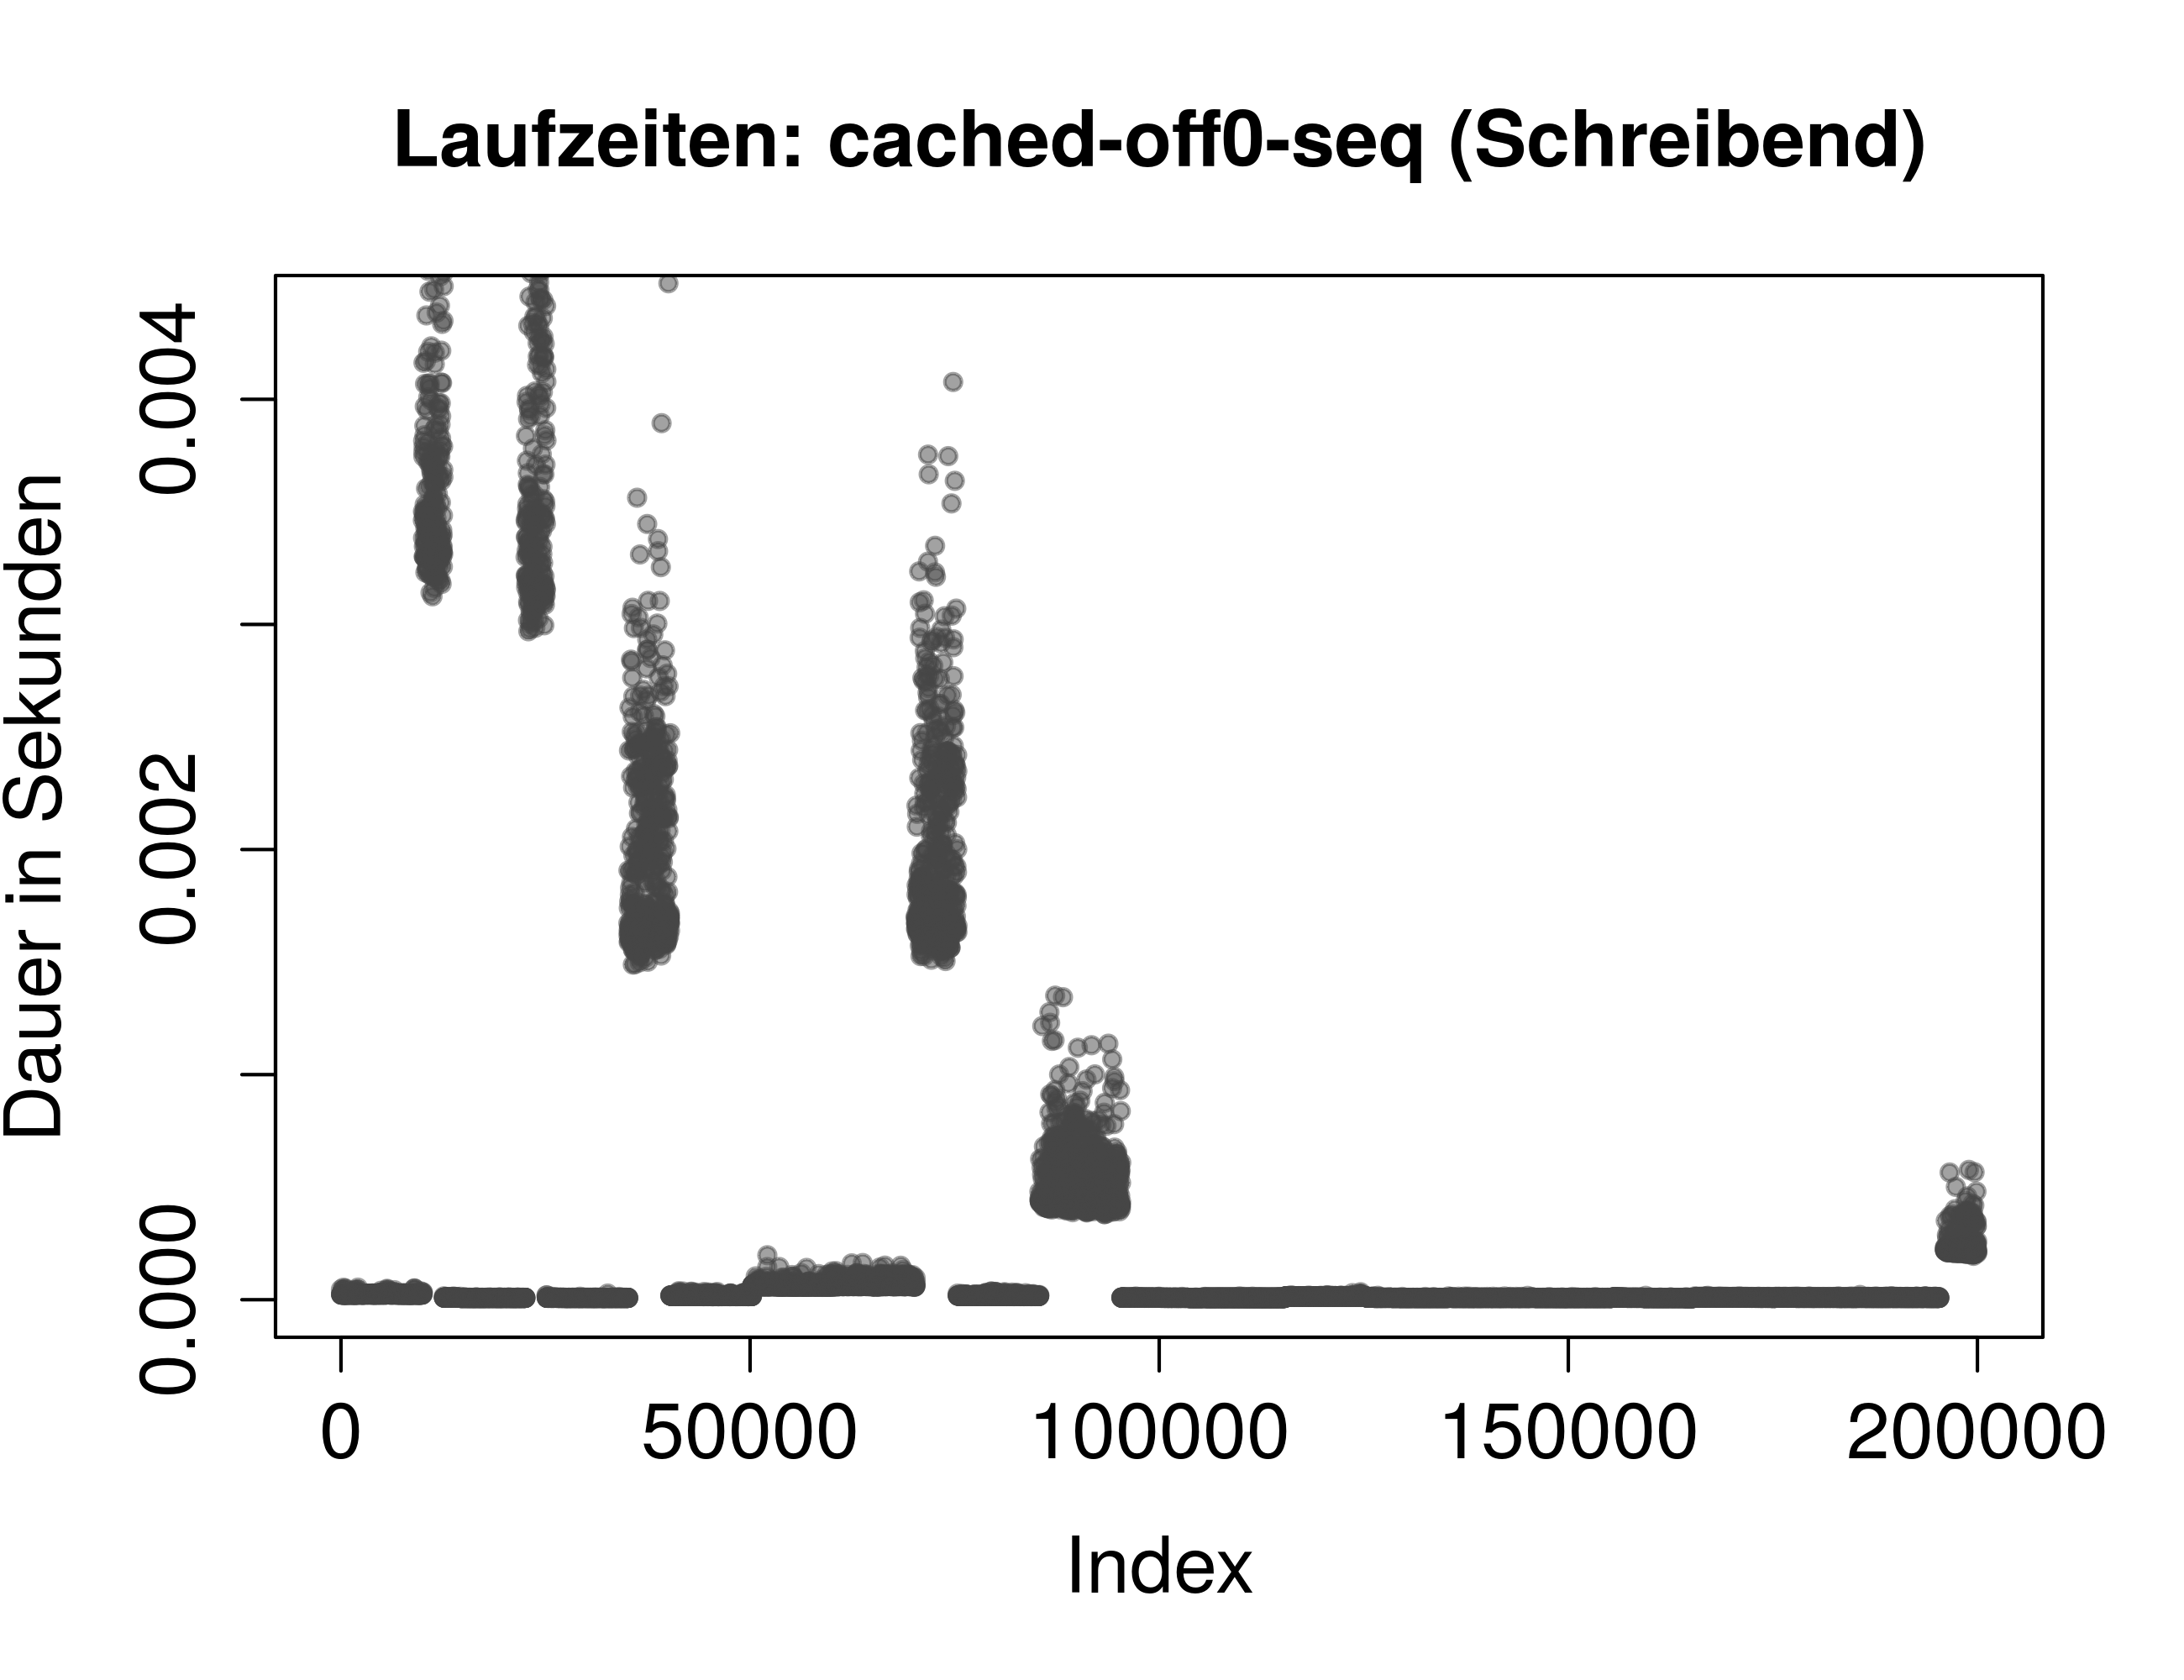
\includegraphics[width=.43\textwidth]{Bilder/Plots/exploration/plot_Duration_write_seq.png}
	}\\
	\subfloat{
		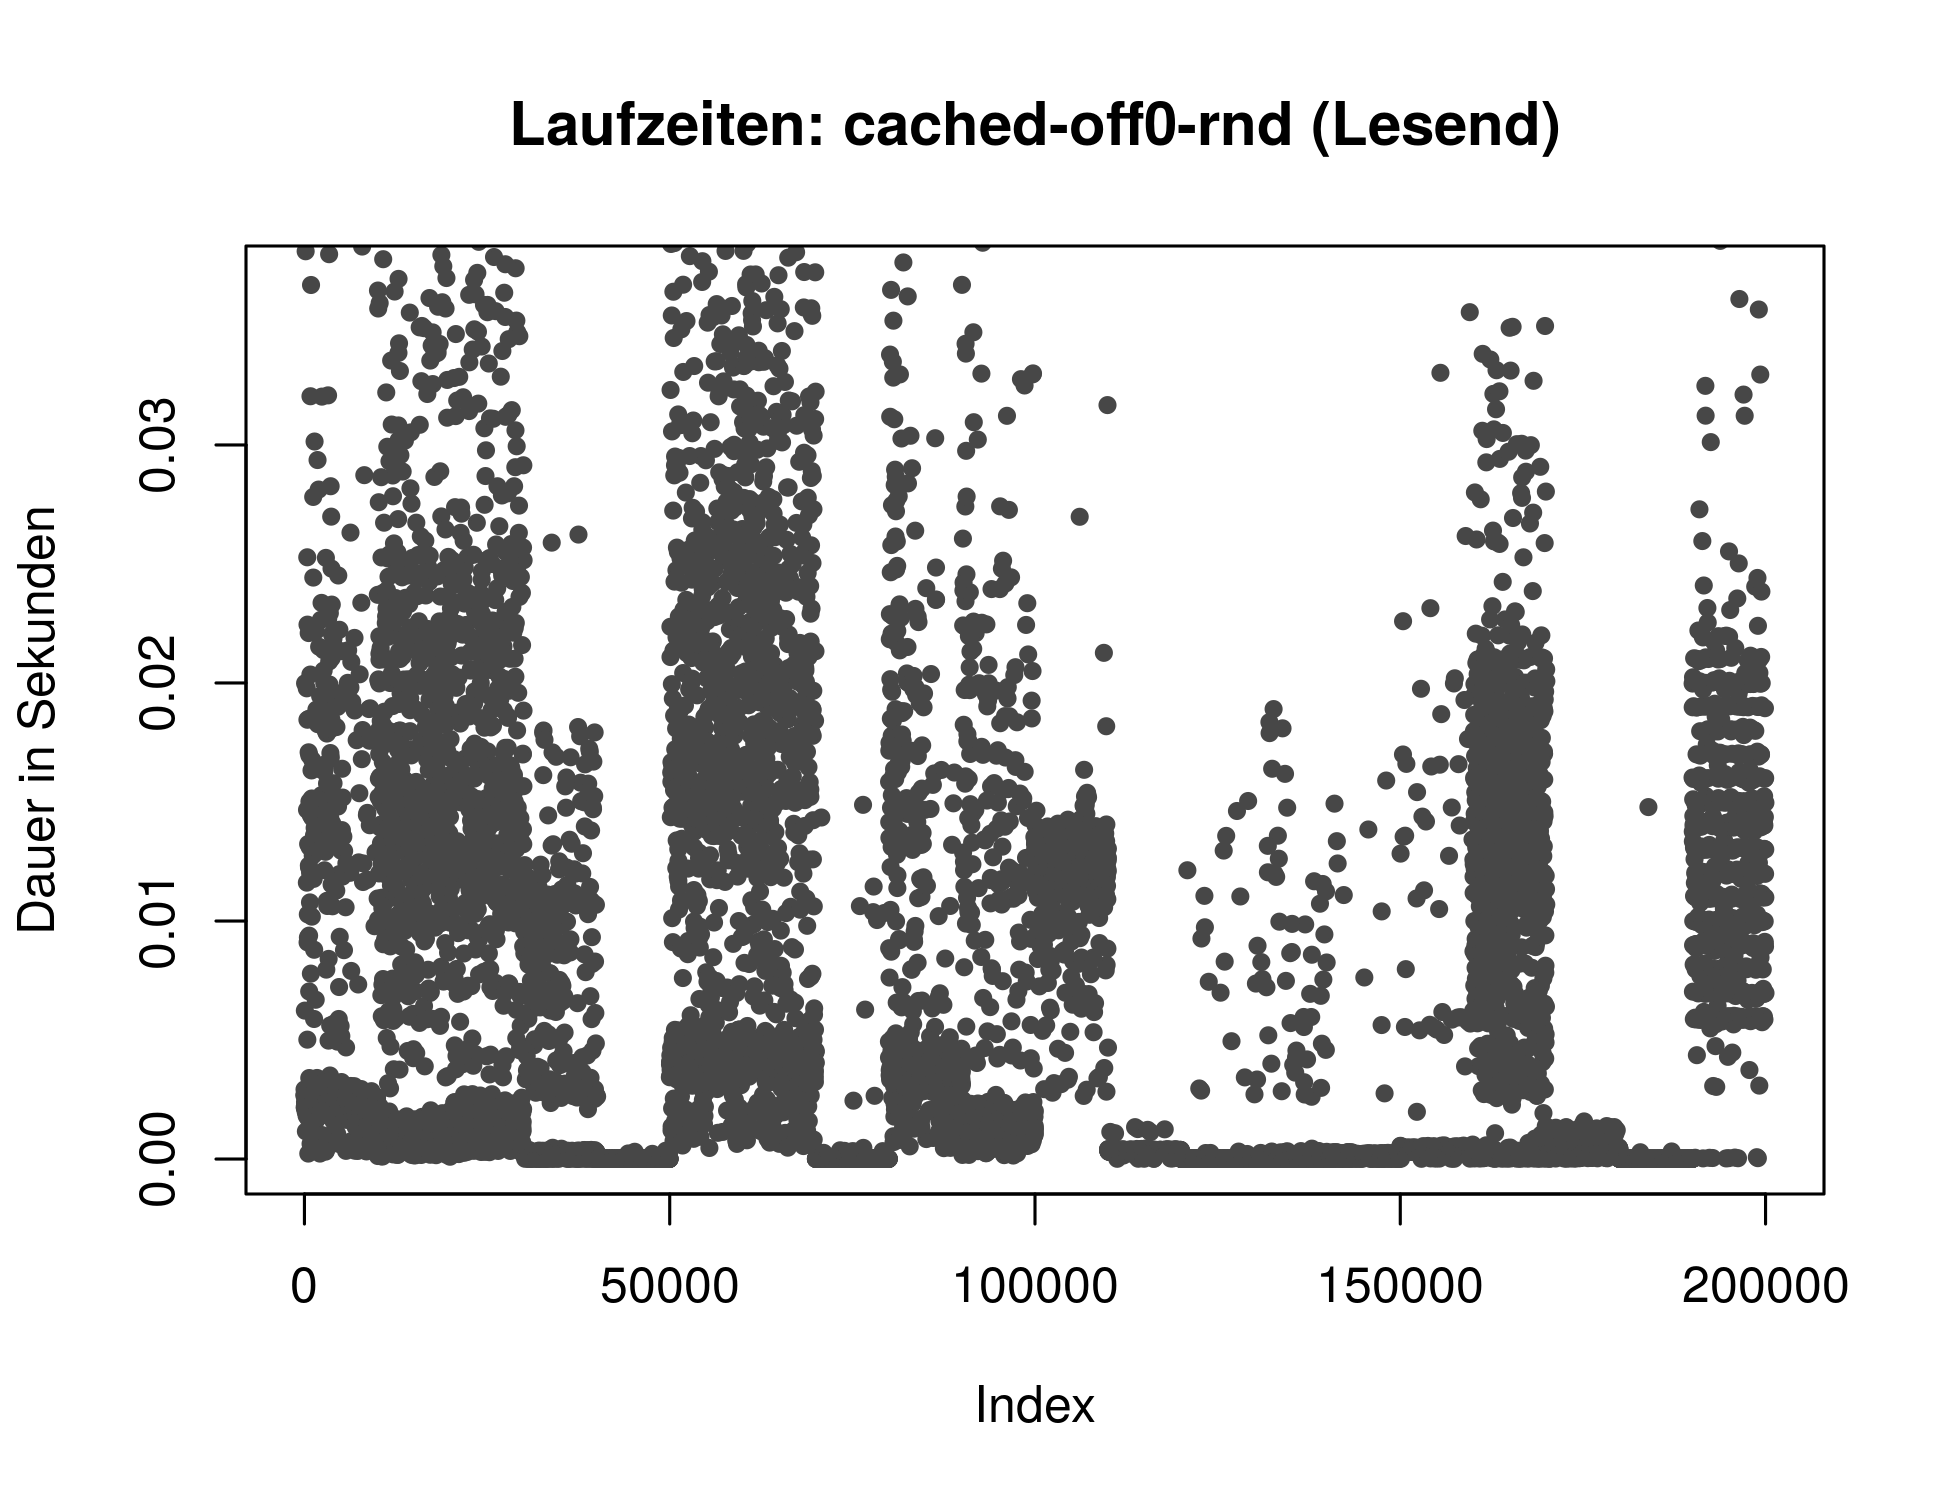
\includegraphics[width=.43\textwidth]{Bilder/Plots/exploration/plot_Duration_read_rnd.png}
	}
	\hfill
	\subfloat{
		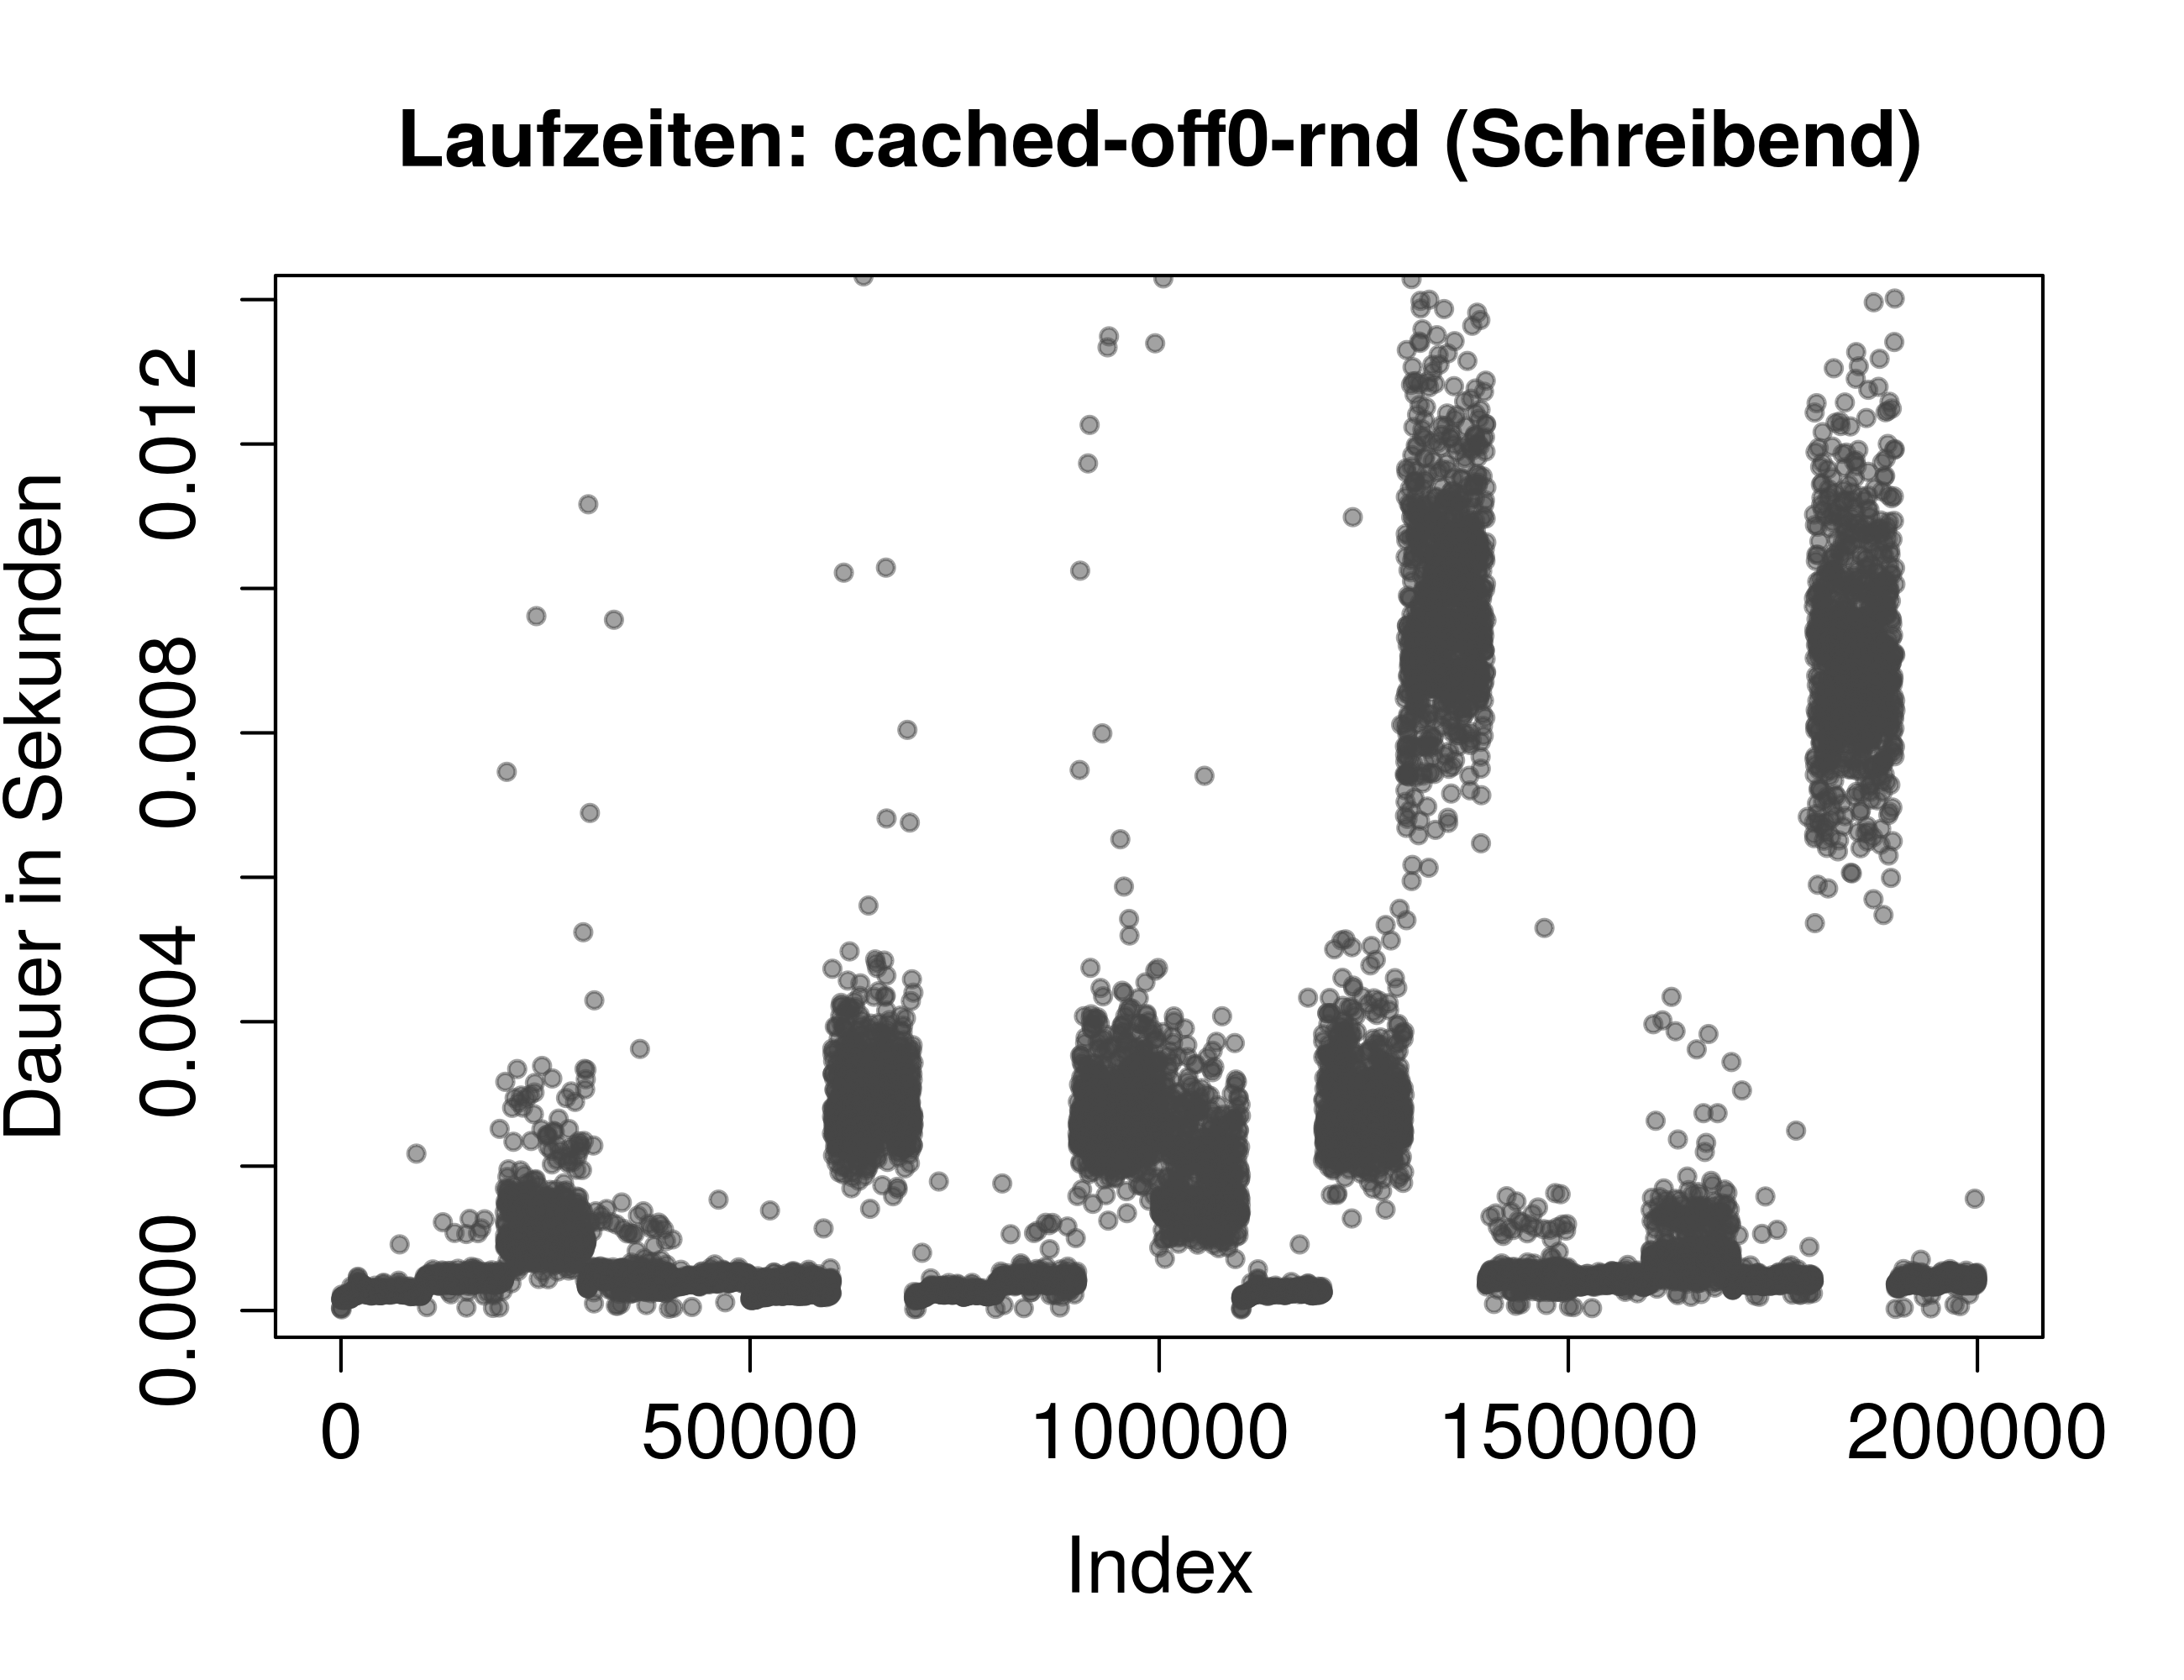
\includegraphics[width=.43\textwidth]{Bilder/Plots/exploration/plot_Duration_write_rnd.png}
	}		
	\caption{Messungen der Laufzeiten als Zeitreihe dargestellt, Index ist die Nummer der Messung}
	\label{Laufzeiten_Zeitreihe}
\end{figure} 

Wenn die Messpunkte nach der Laufzeit sortiert sind, kann die Verteilung Daten besser betrachtet werden. Die logarithmische Skalierung der Y-Achse entzerrt die Punkte (\ref{Laufzeiten_Sortiert}).

\begin{figure}
	\subfloat{
		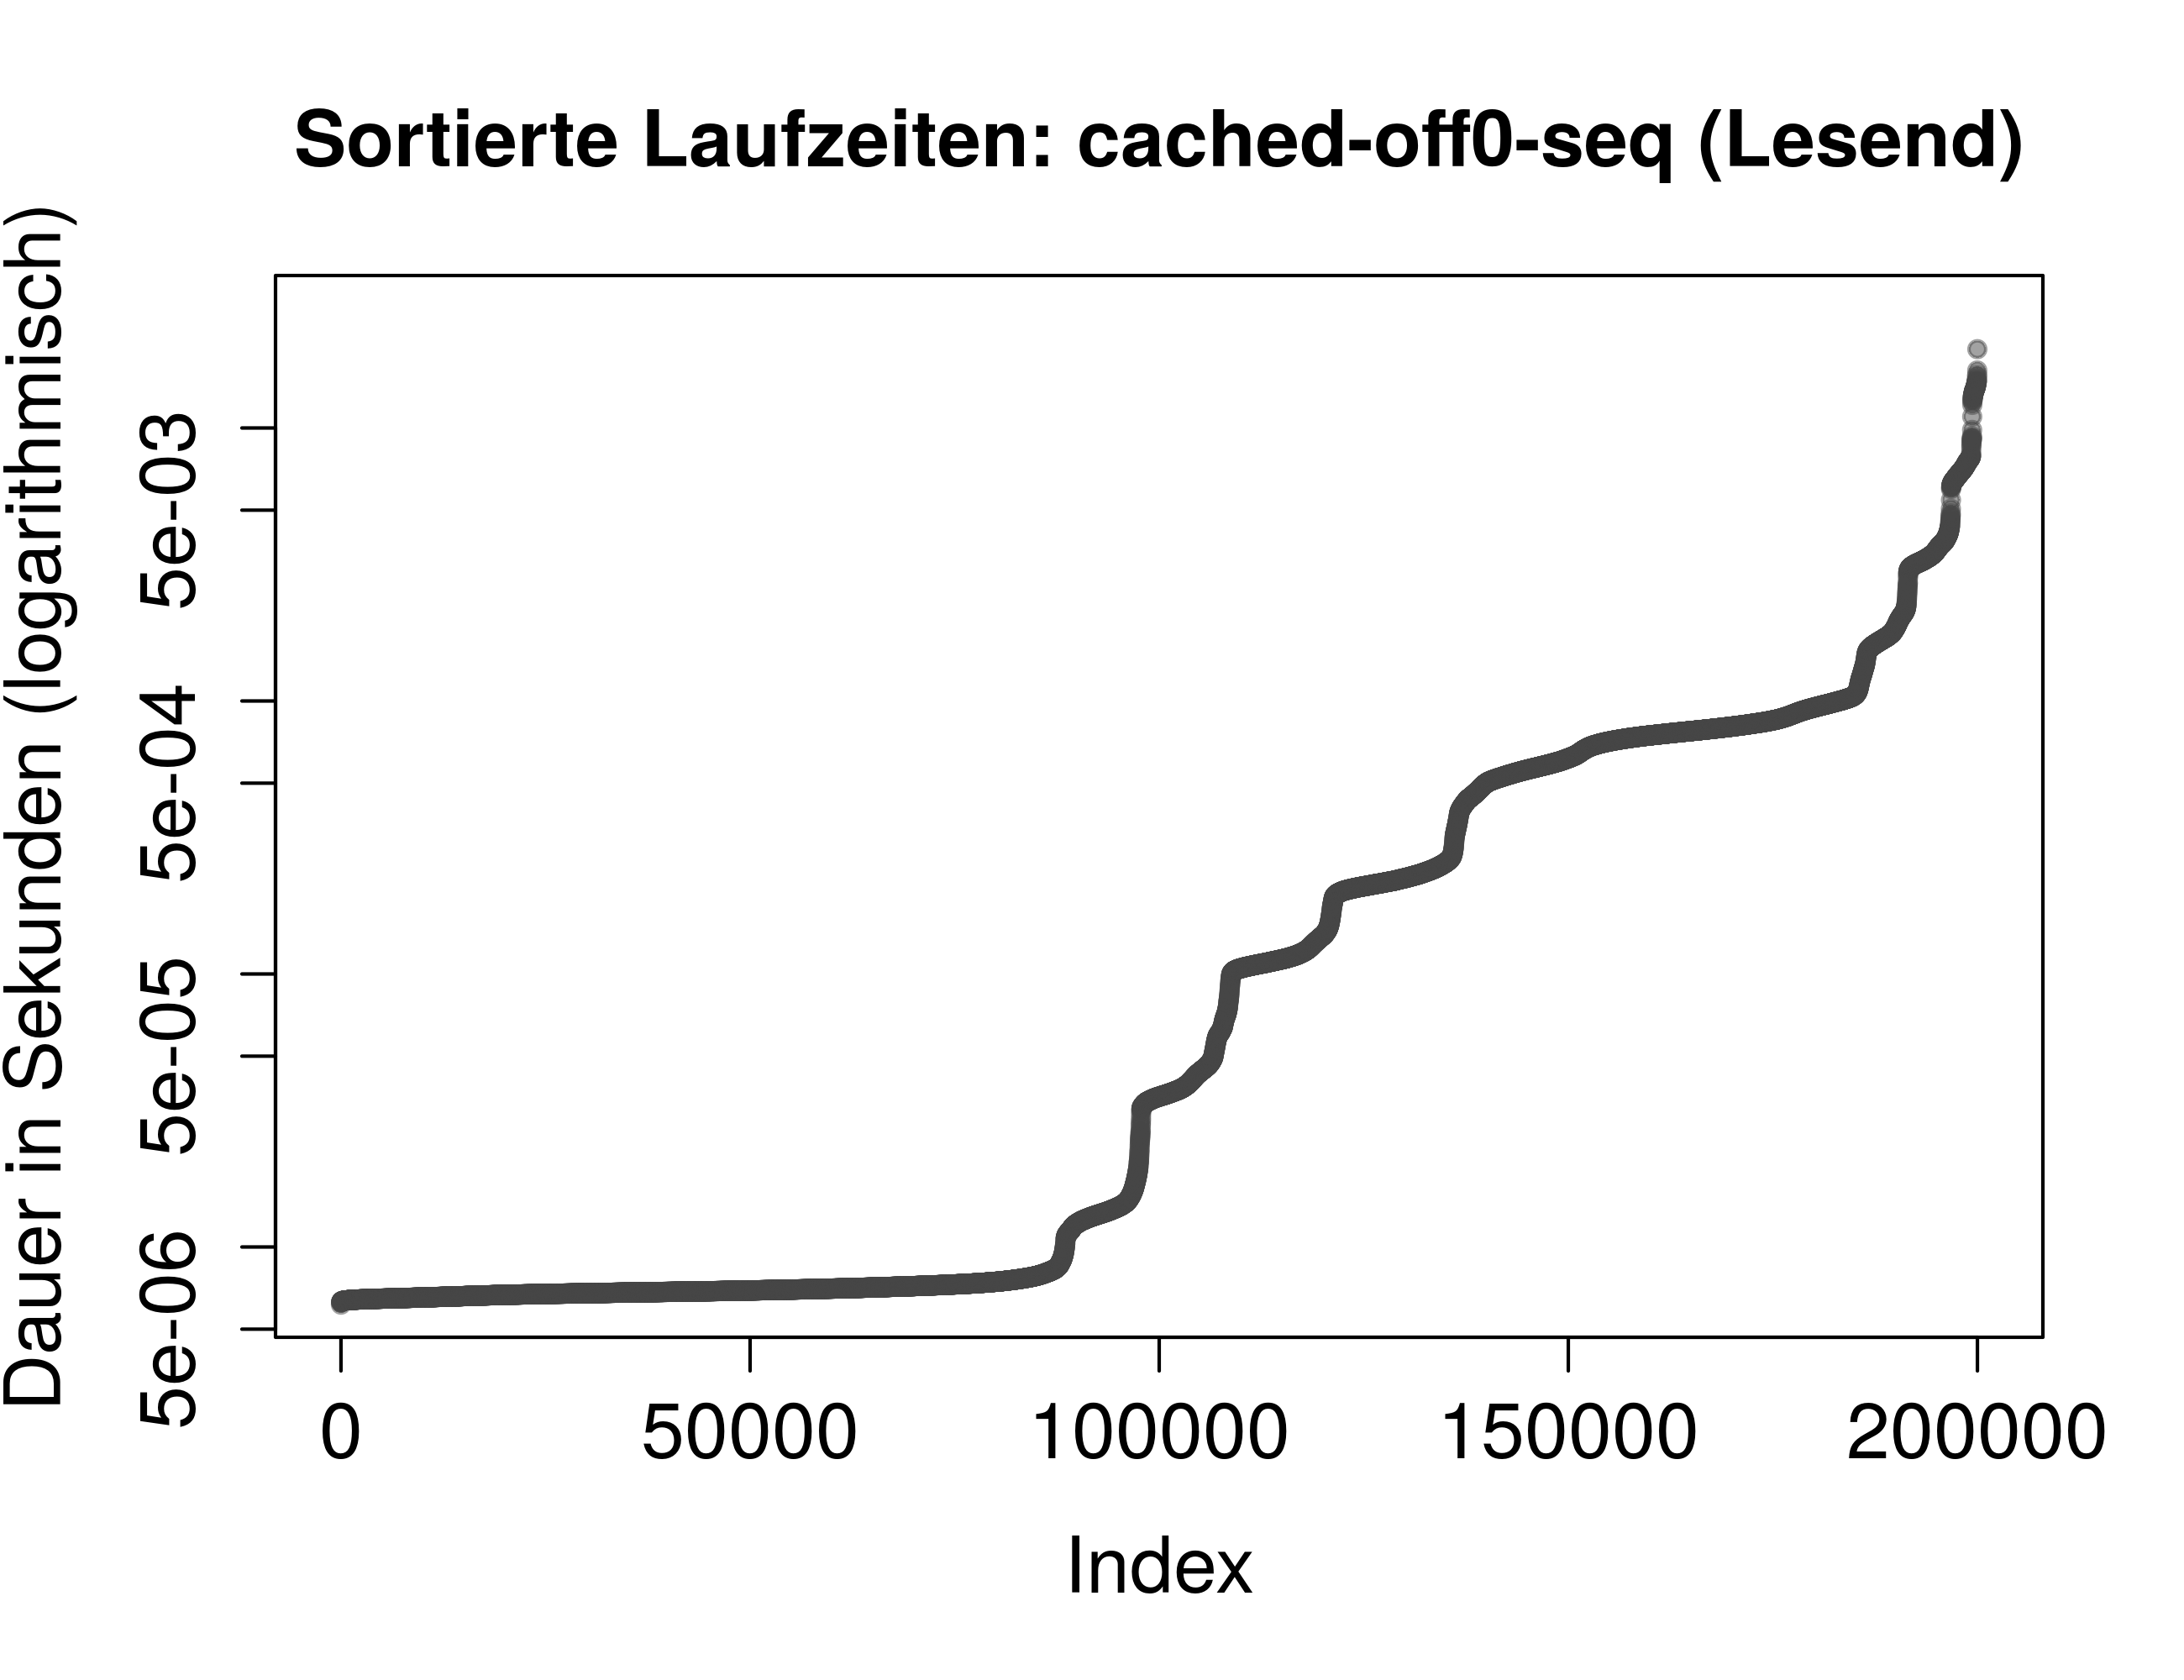
\includegraphics[width=.43\textwidth]{Bilder/Plots/exploration/plot_DurationSorted_read_seq.png}
	}
	\hfill
	\subfloat{
		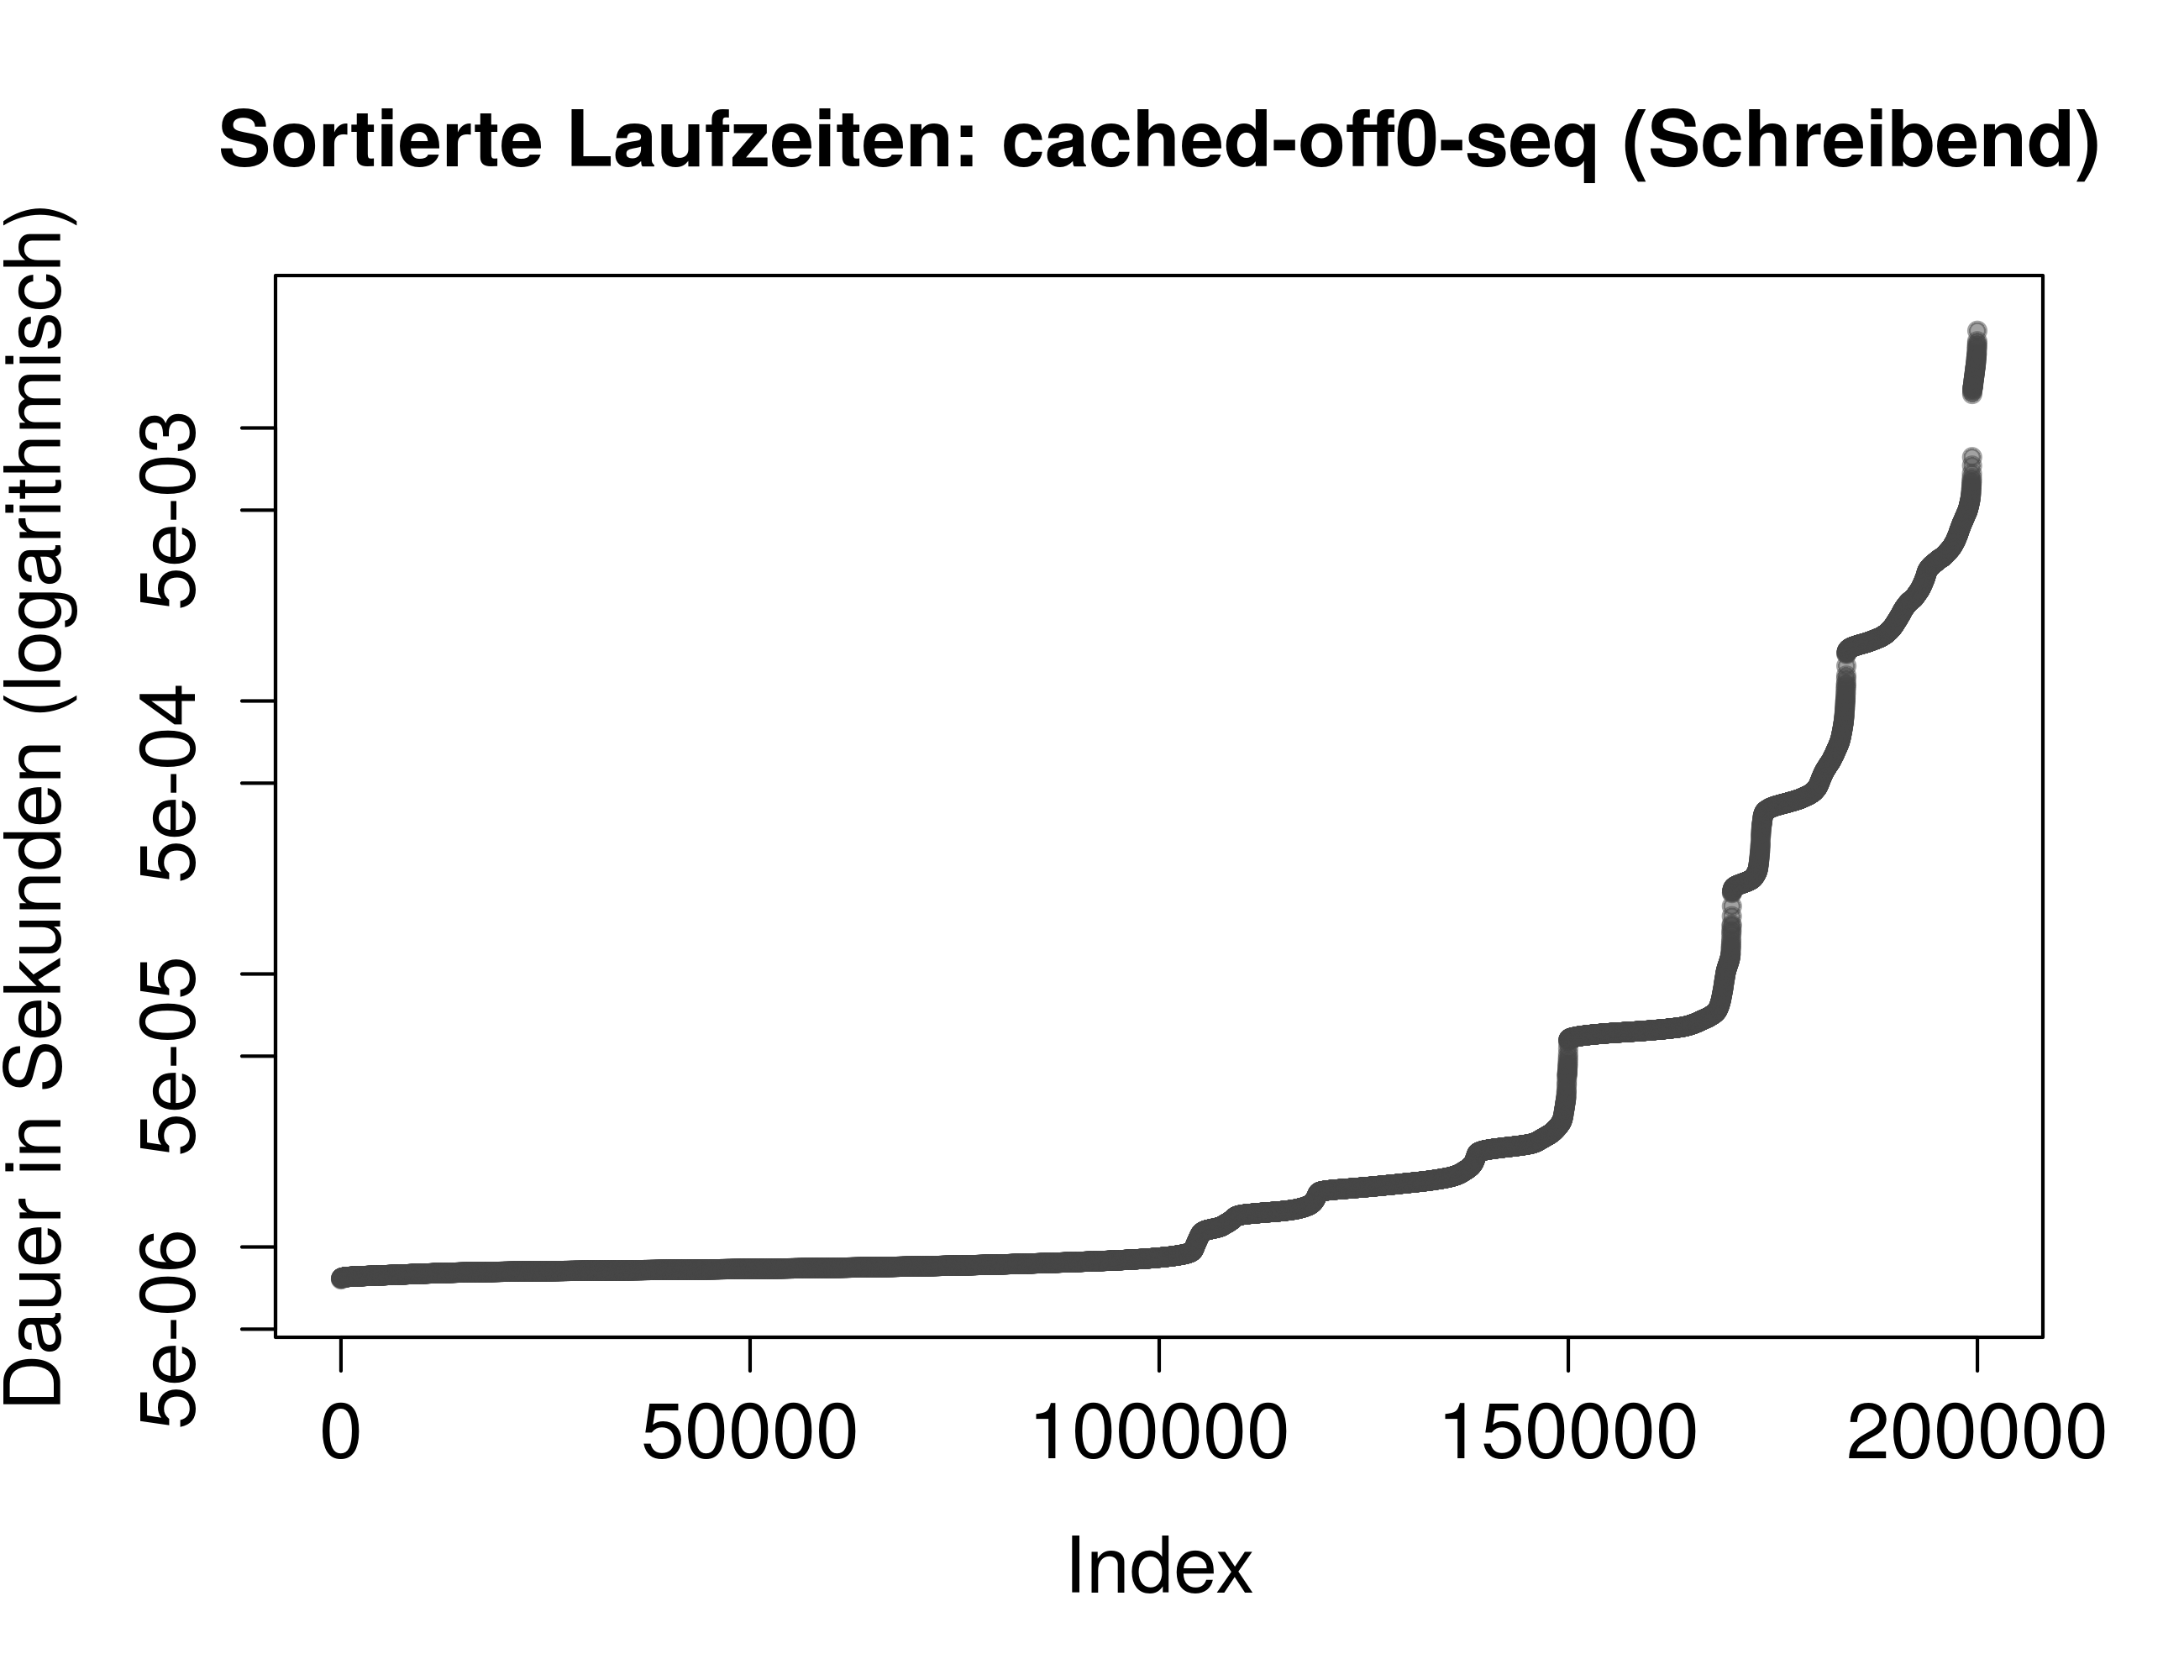
\includegraphics[width=.43\textwidth]{Bilder/Plots/exploration/plot_DurationSorted_write_seq.png}
	}\\
	\subfloat{
		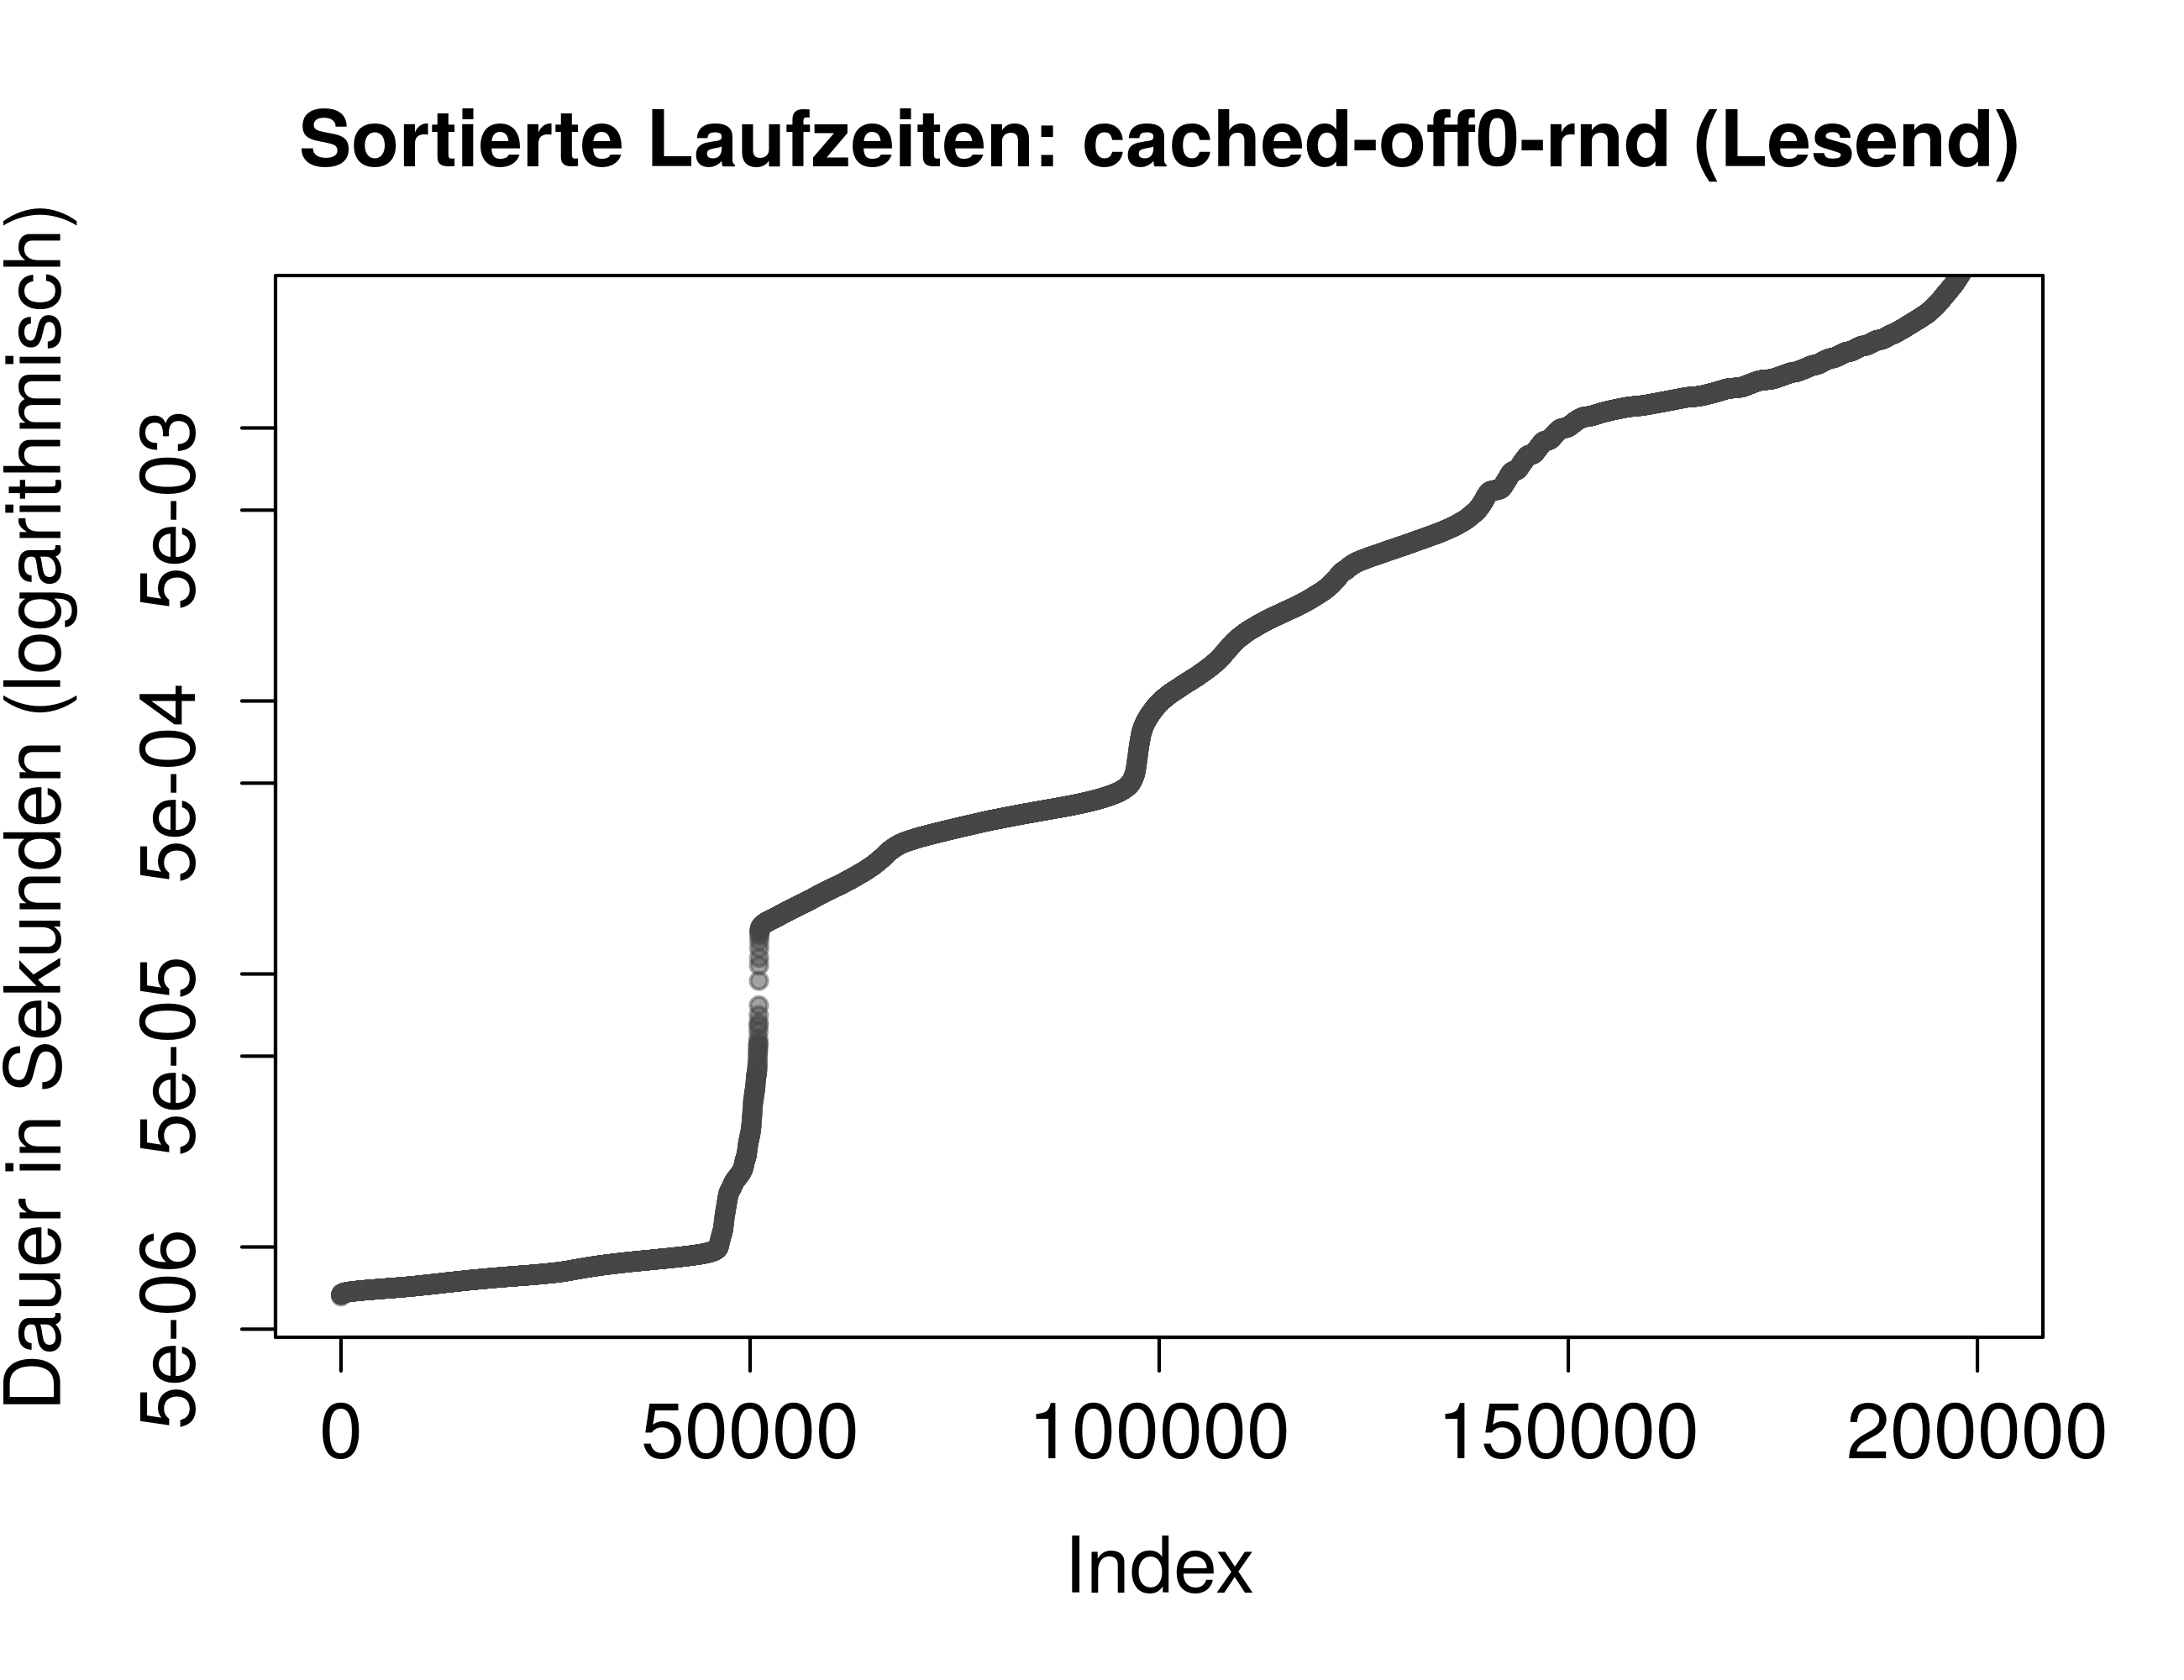
\includegraphics[width=.43\textwidth]{Bilder/Plots/exploration/plot_DurationSorted_read_rnd.png}
	}
	\hfill
	\subfloat{
		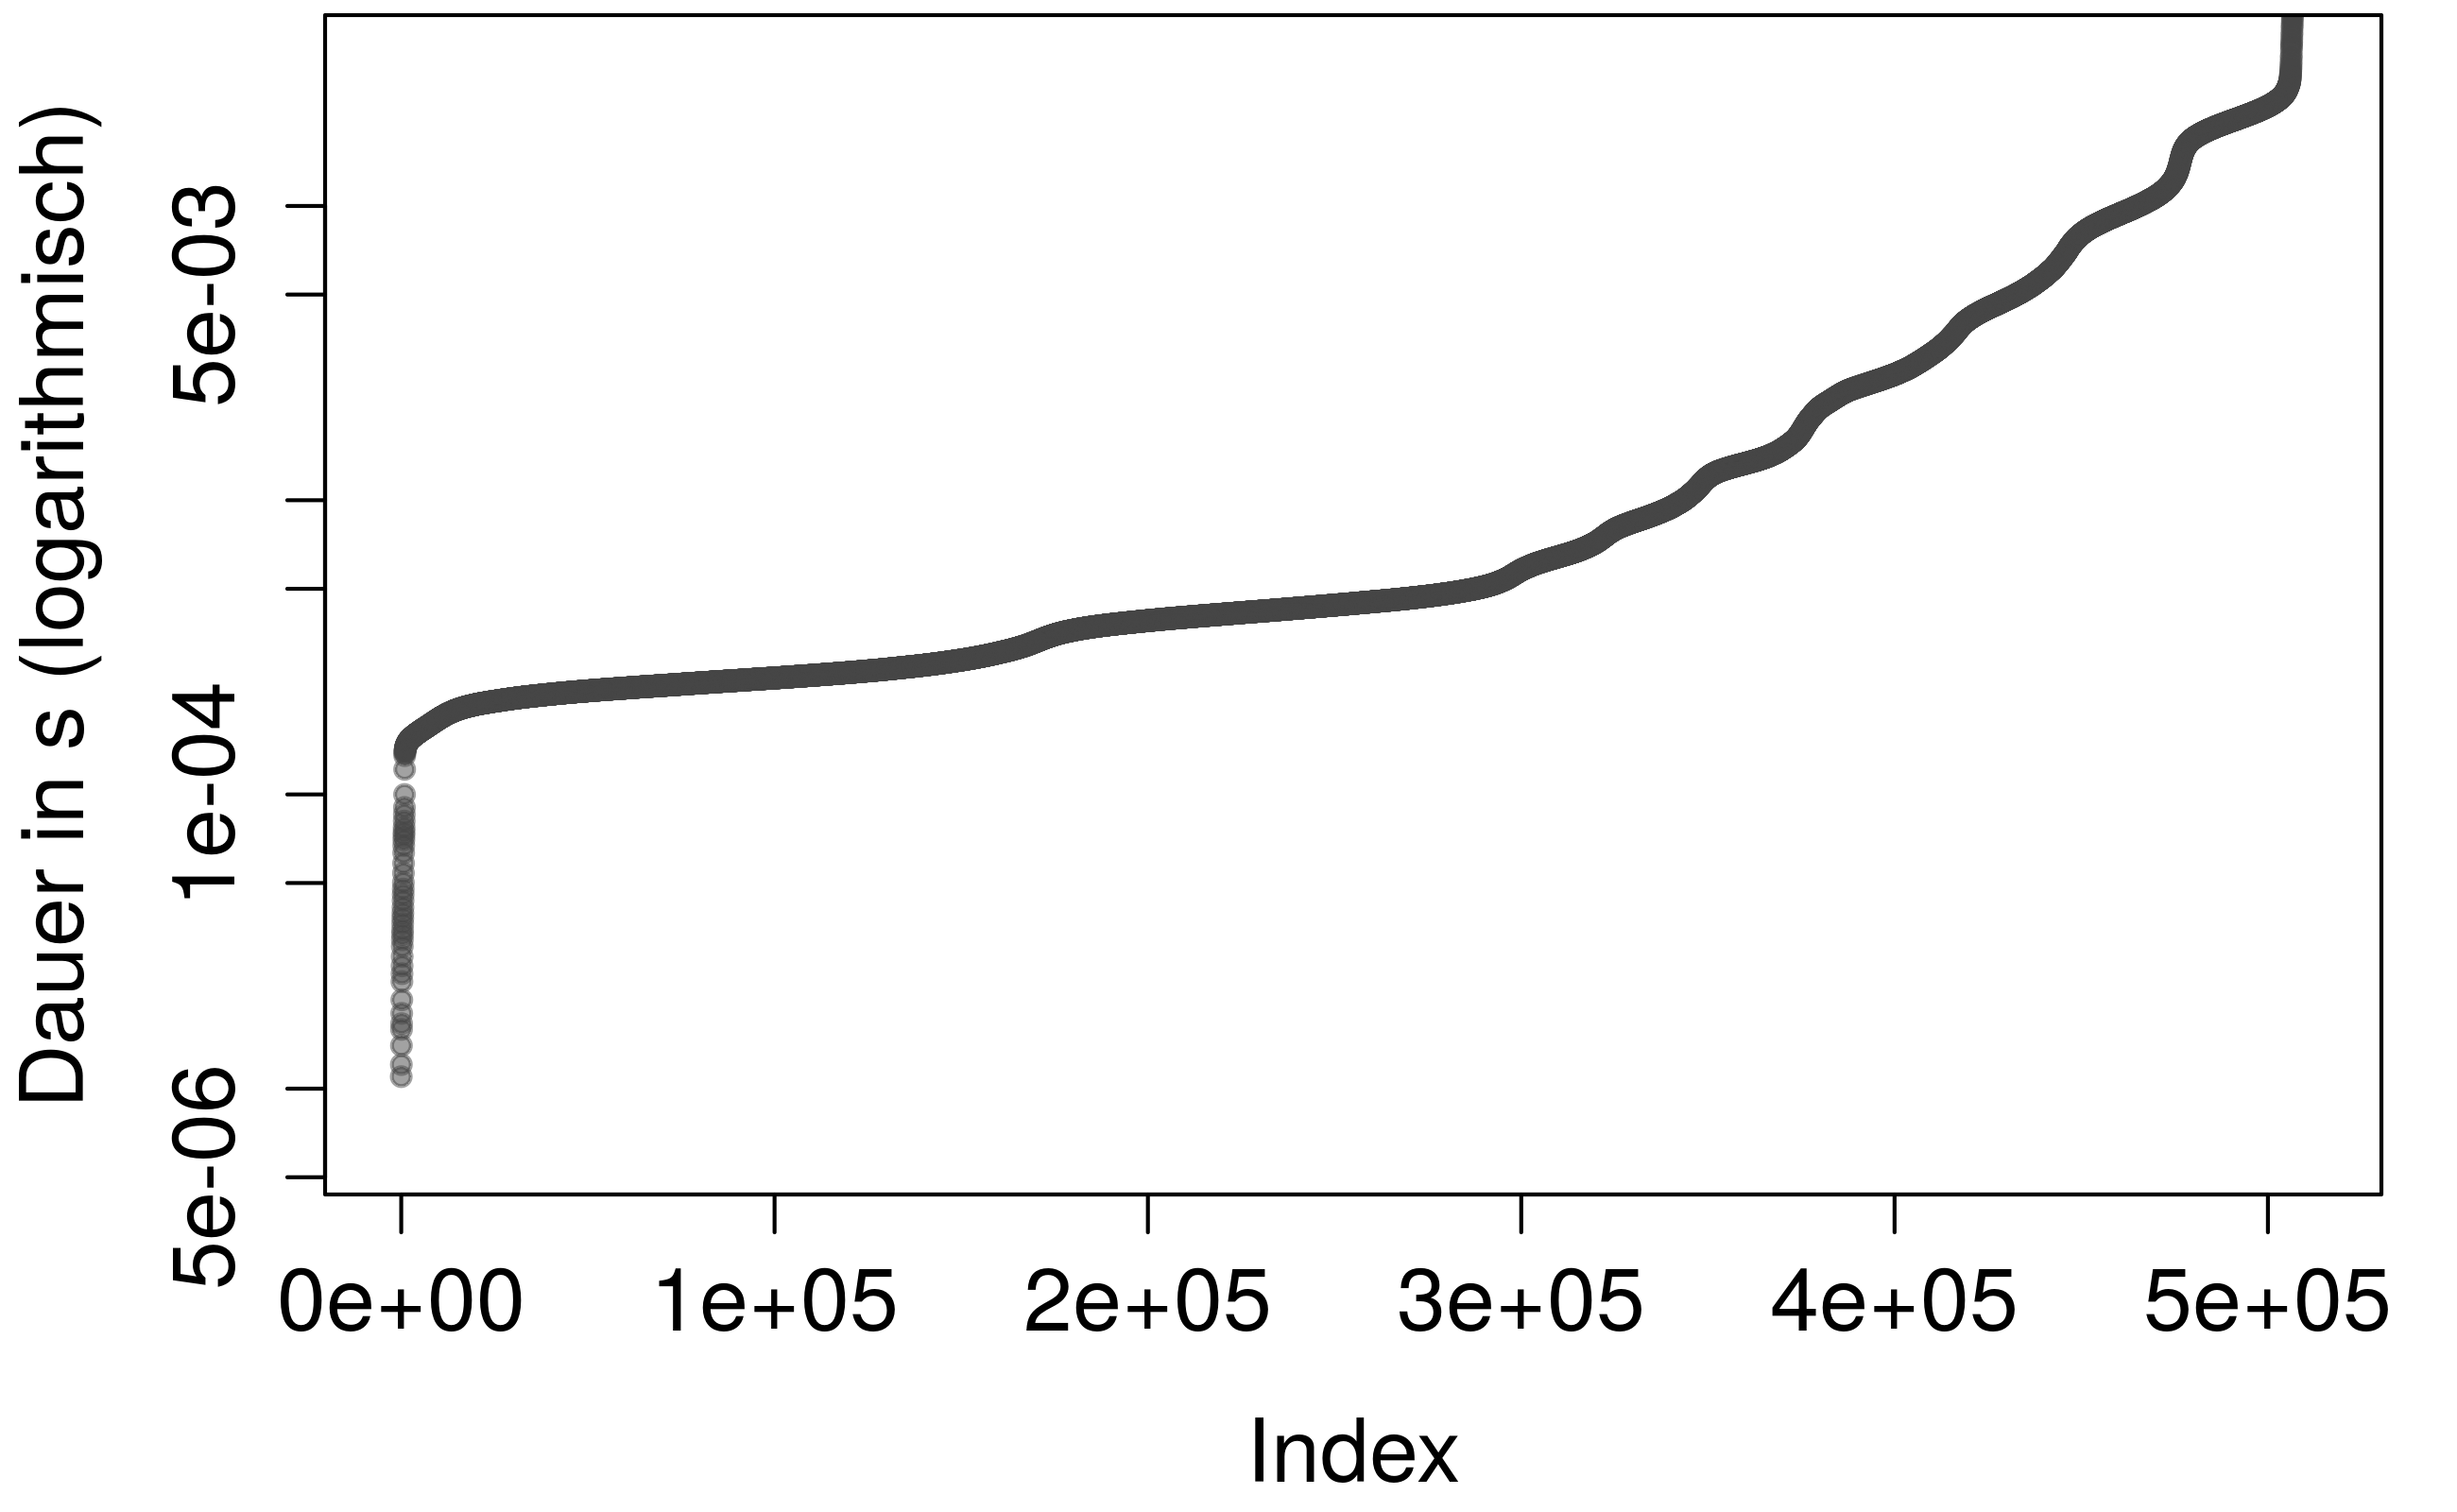
\includegraphics[width=.43\textwidth]{Bilder/Plots/exploration/plot_DurationSorted_write_rnd.png}
	}		
	\caption{Messungen der Laufzeiten sortiert dargestellt (logarithmische Y-Achse)}
	\label{Laufzeiten_Sortiert}
\end{figure} 

Zum Vergleich werden die Laufzeiten in \ref{Laufzeiten_Sortiert_nolog} ohne logarithmische Y-Achse dargestellt. Aufgrund der Häufung von Messungen mit sehr kurzer Laufzeit sind etwa die ersten 100.000 Werte in dieser Darstellung nicht zu unterscheiden. Aus diesem Grund werden die Laufzeiten (und Zugriffsgrößen zur Erhaltung der Korrelation) für die höheren Modelle zum Lernen logarithmiert. Da die neuronalen Netze versuchen den Modellfehler zu minimieren würde es ansonsten eine Tendenz dazu geben, die Messungen mit längerer Laufzeit korrekt zu lernen. Während für die kürzeren Laufzeiten für den internen Modellfehler unwichtiger wären. Ein ungenaues Lernen der Messungen mit kürzeren Laufzeiten würde sich  nicht in einer absoluten Metrik, sondern nur in einer Relativen niederschlagen.

\begin{figure}
	\subfloat{
		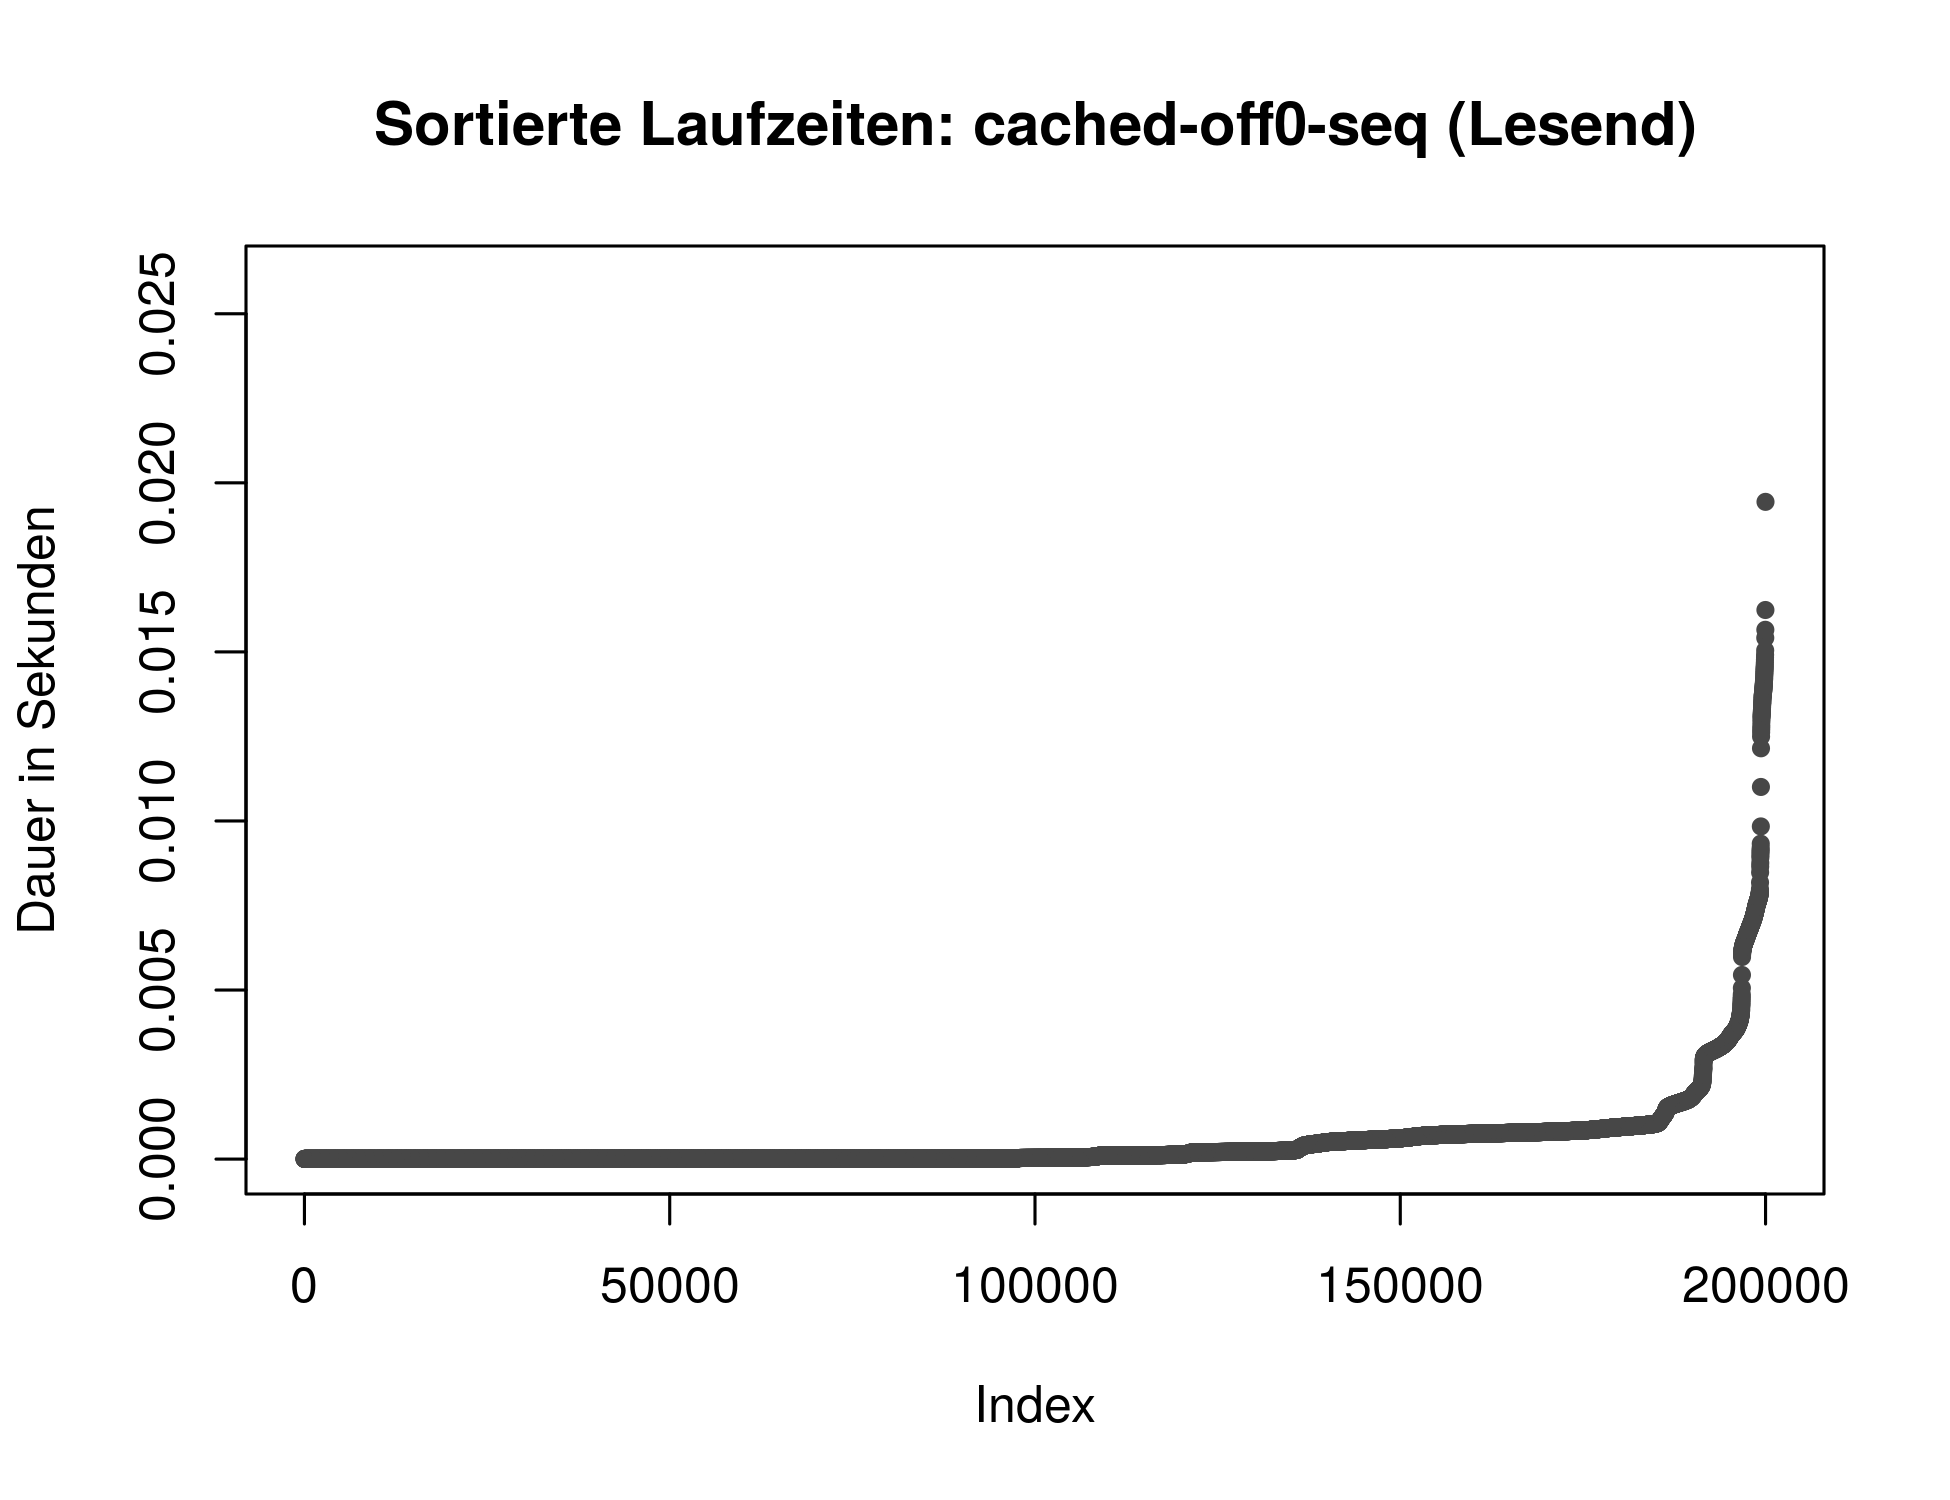
\includegraphics[width=.43\textwidth]{Bilder/Plots/exploration/plot_DurationSorted_read_seq_nolog.png}
	}
	\hfill
	\subfloat{
		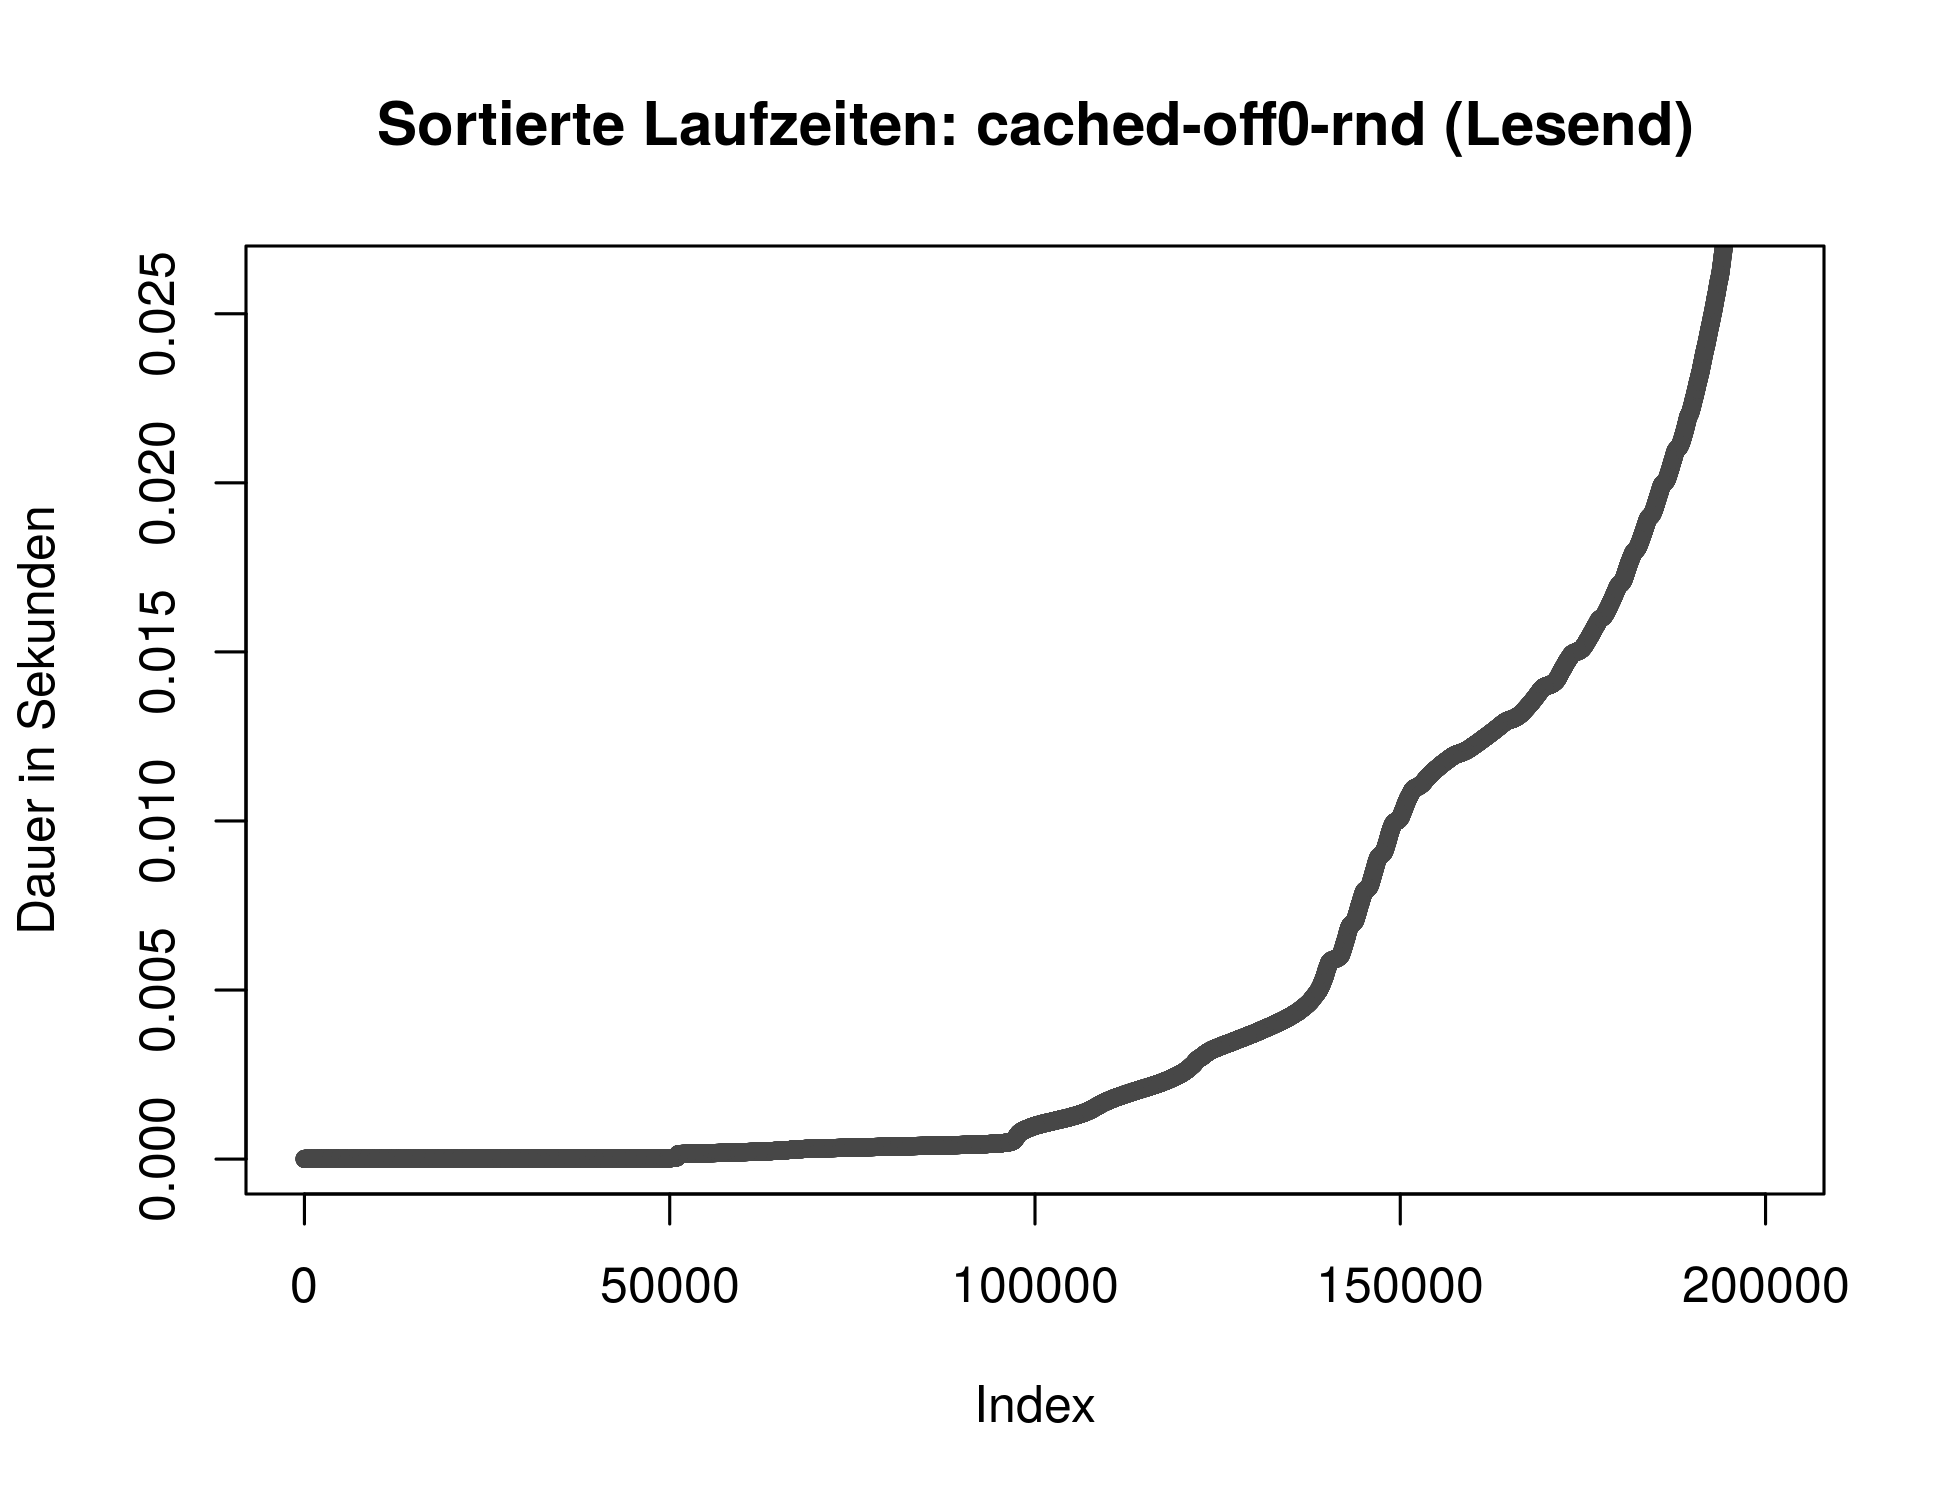
\includegraphics[width=.43\textwidth]{Bilder/Plots/exploration/plot_DurationSorted_read_rnd_nolog.png}
	}			
	\caption{Messungen der Laufzeiten sortiert dargestellt ohne Logarithmus}
	\label{Laufzeiten_Sortiert_nolog}
\end{figure} 

Als Ausreißer werden für alle \textbf{Attribut-Sets} die Messungen mit den $10\%$ kürzesten und längsten Laufzeiten behandelt. Die Verteilung der Ausreißer ist in \ref{fig:ausreisser} erkennen.\\
Am Verhalten der Ausreißer lässt sich gut unterscheiden, ob es sich um den sequentiellen oder den randomisierten Datensatz handelt. Bei cached-off0-seq befinden sich die Ausreißer gerade an den oberen und unteren Enden einer Ansammlung von Punkten. Da alle Punkte innerhalb der Ansammlung zu einem Attribut-Set gehören muss sich gerade dieses Bild ergeben. Dagegen sind die roten Punkte bei cached-off0-rnd unregelmäßiger verteilt. Da die Ausreißer als zweites in den Graphen gezeichnet wurden, überdecken sie die grauen und erscheinen daher präsenter. (\textbf{Sind die Ausreißer hier eher ein Zeichen dafür, dass das System in den Häufungspunkten von Ausreißern besonders schnell oder langsam  agiert hat, oder ist dies durch die Art des Benchmarks bedingt}?)

\begin{figure}
	\subfloat{
		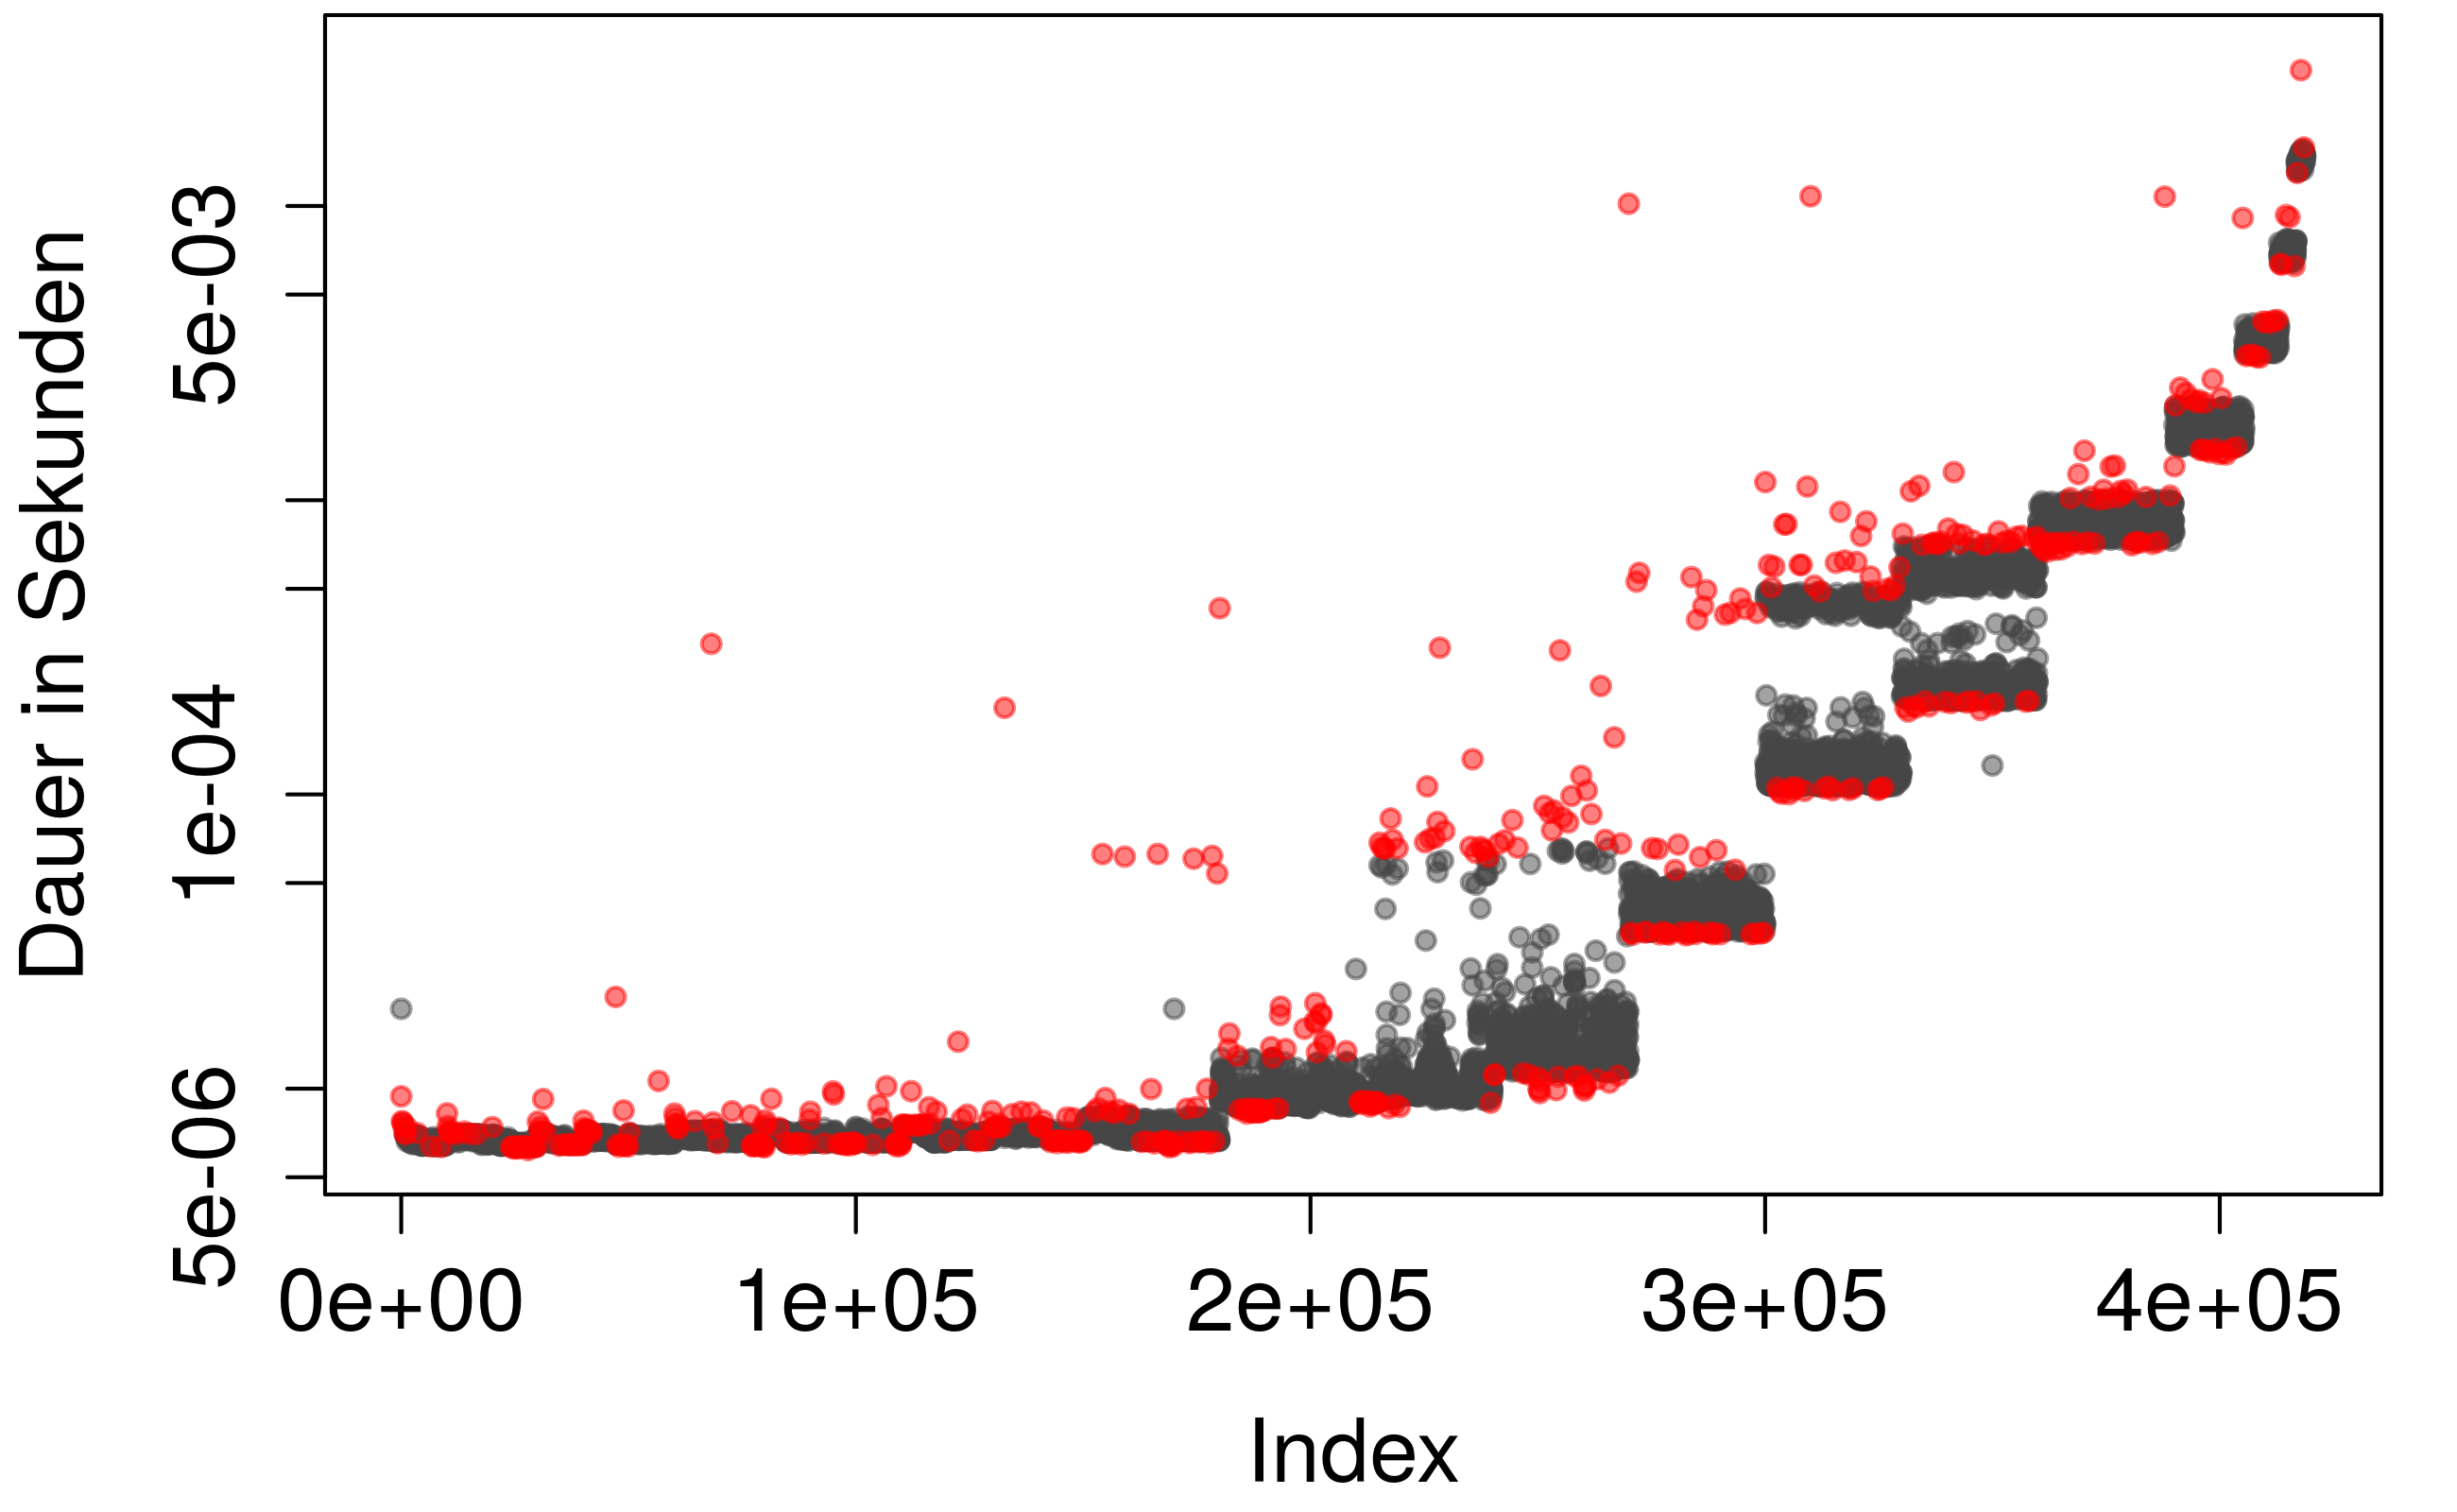
\includegraphics[width=.43\textwidth]{Bilder/Plots/exploration/plot_outlier_read_seq.png}
	}
	\hfill
	\subfloat{
		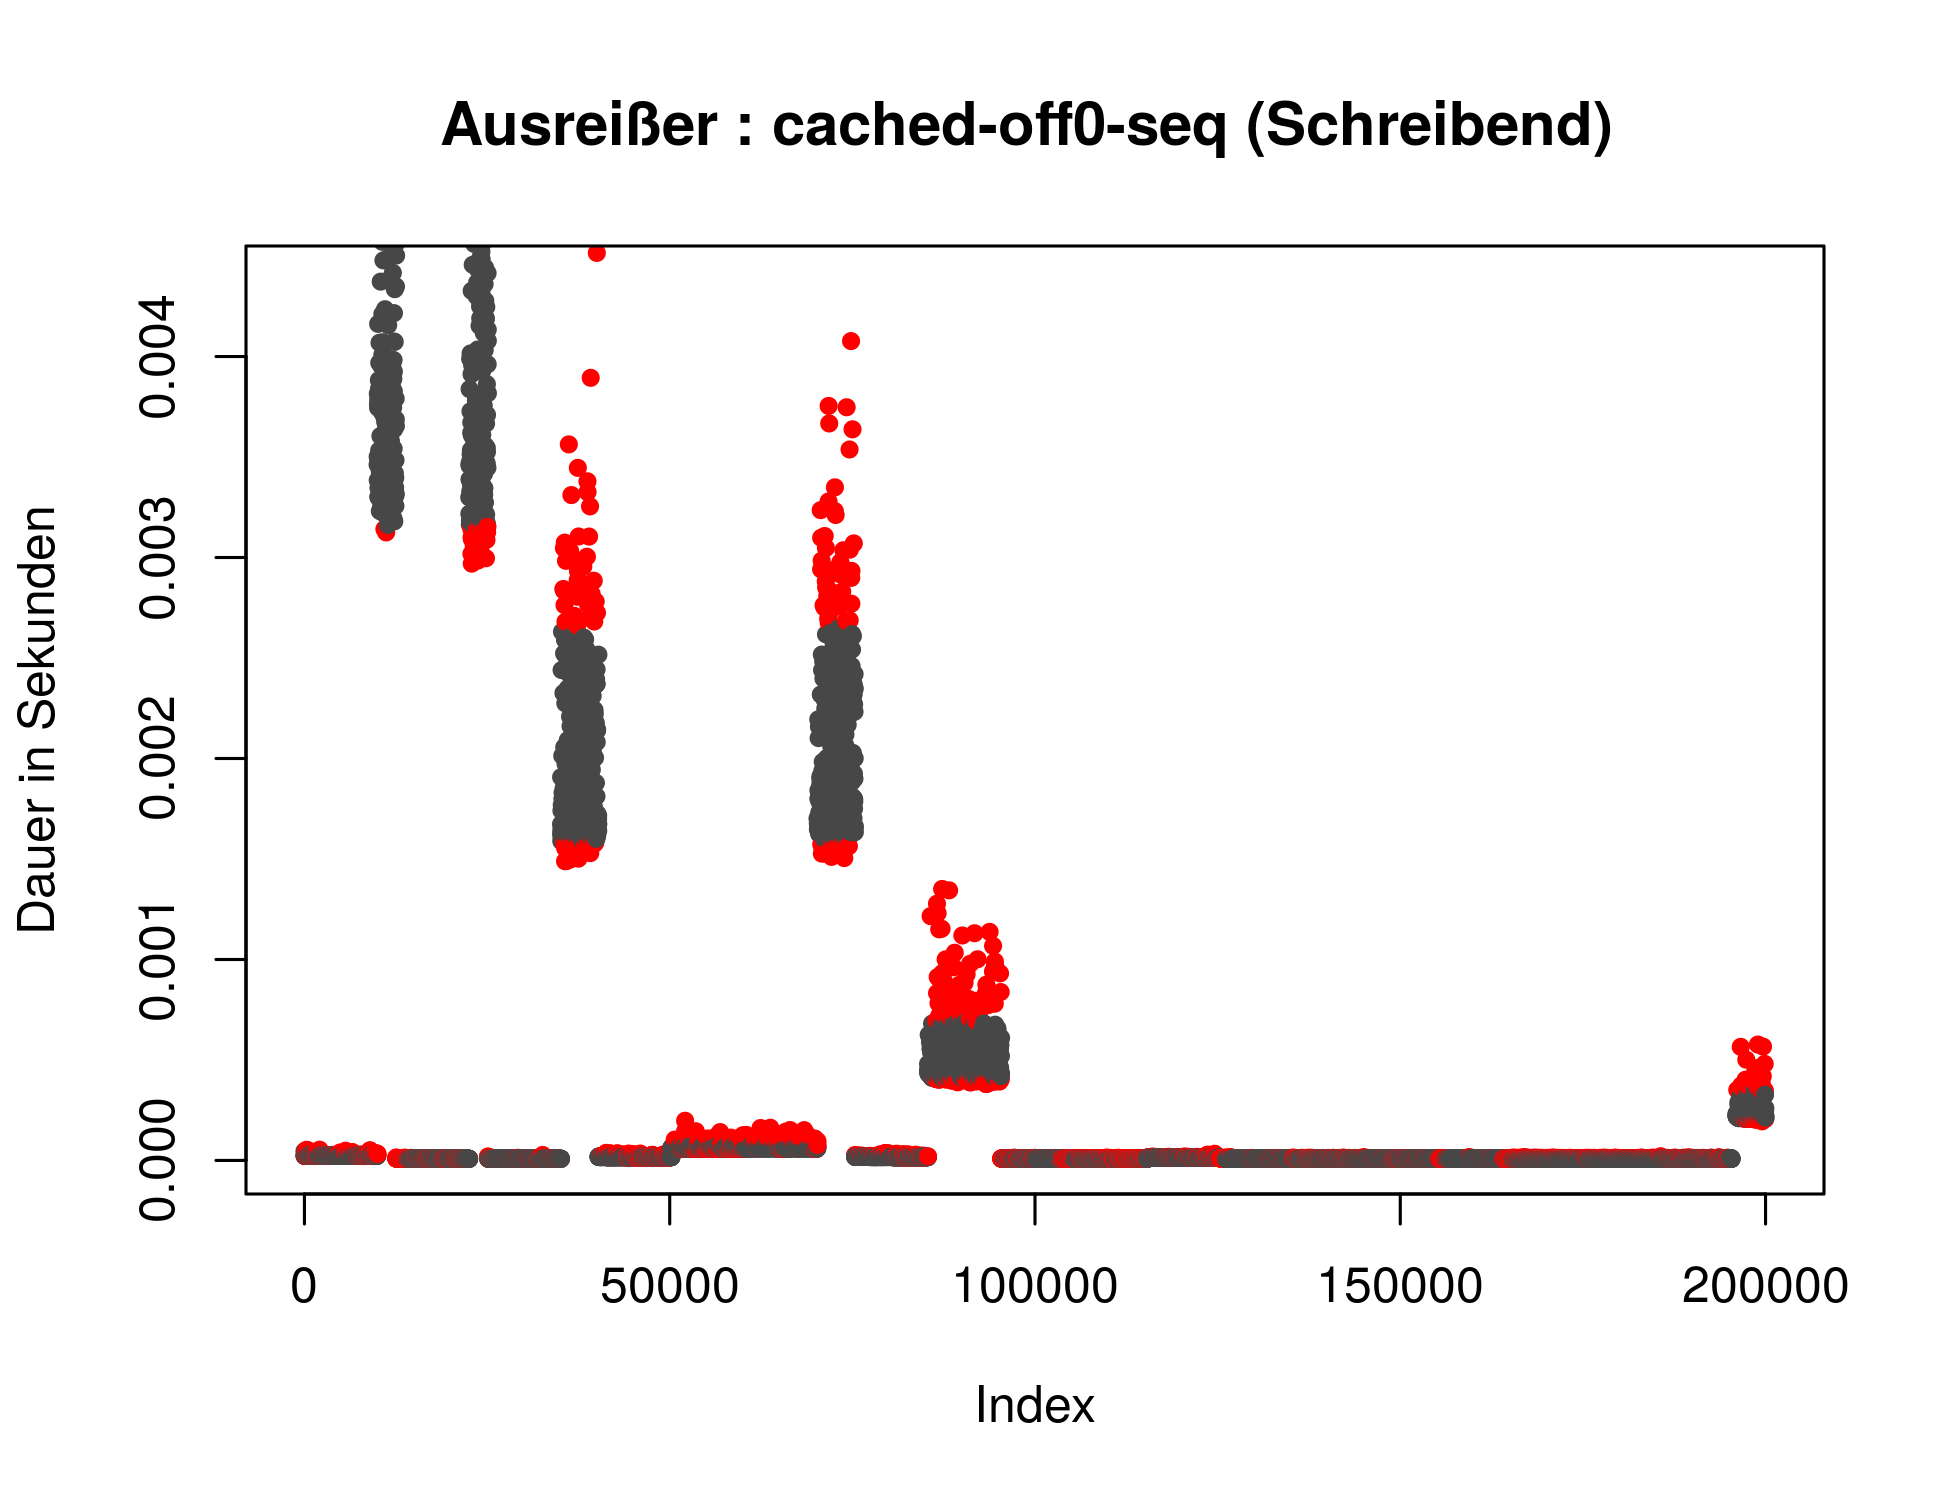
\includegraphics[width=.43\textwidth]{Bilder/Plots/exploration/plot_outlier_write_seq.png}
	}\\
	\subfloat{
		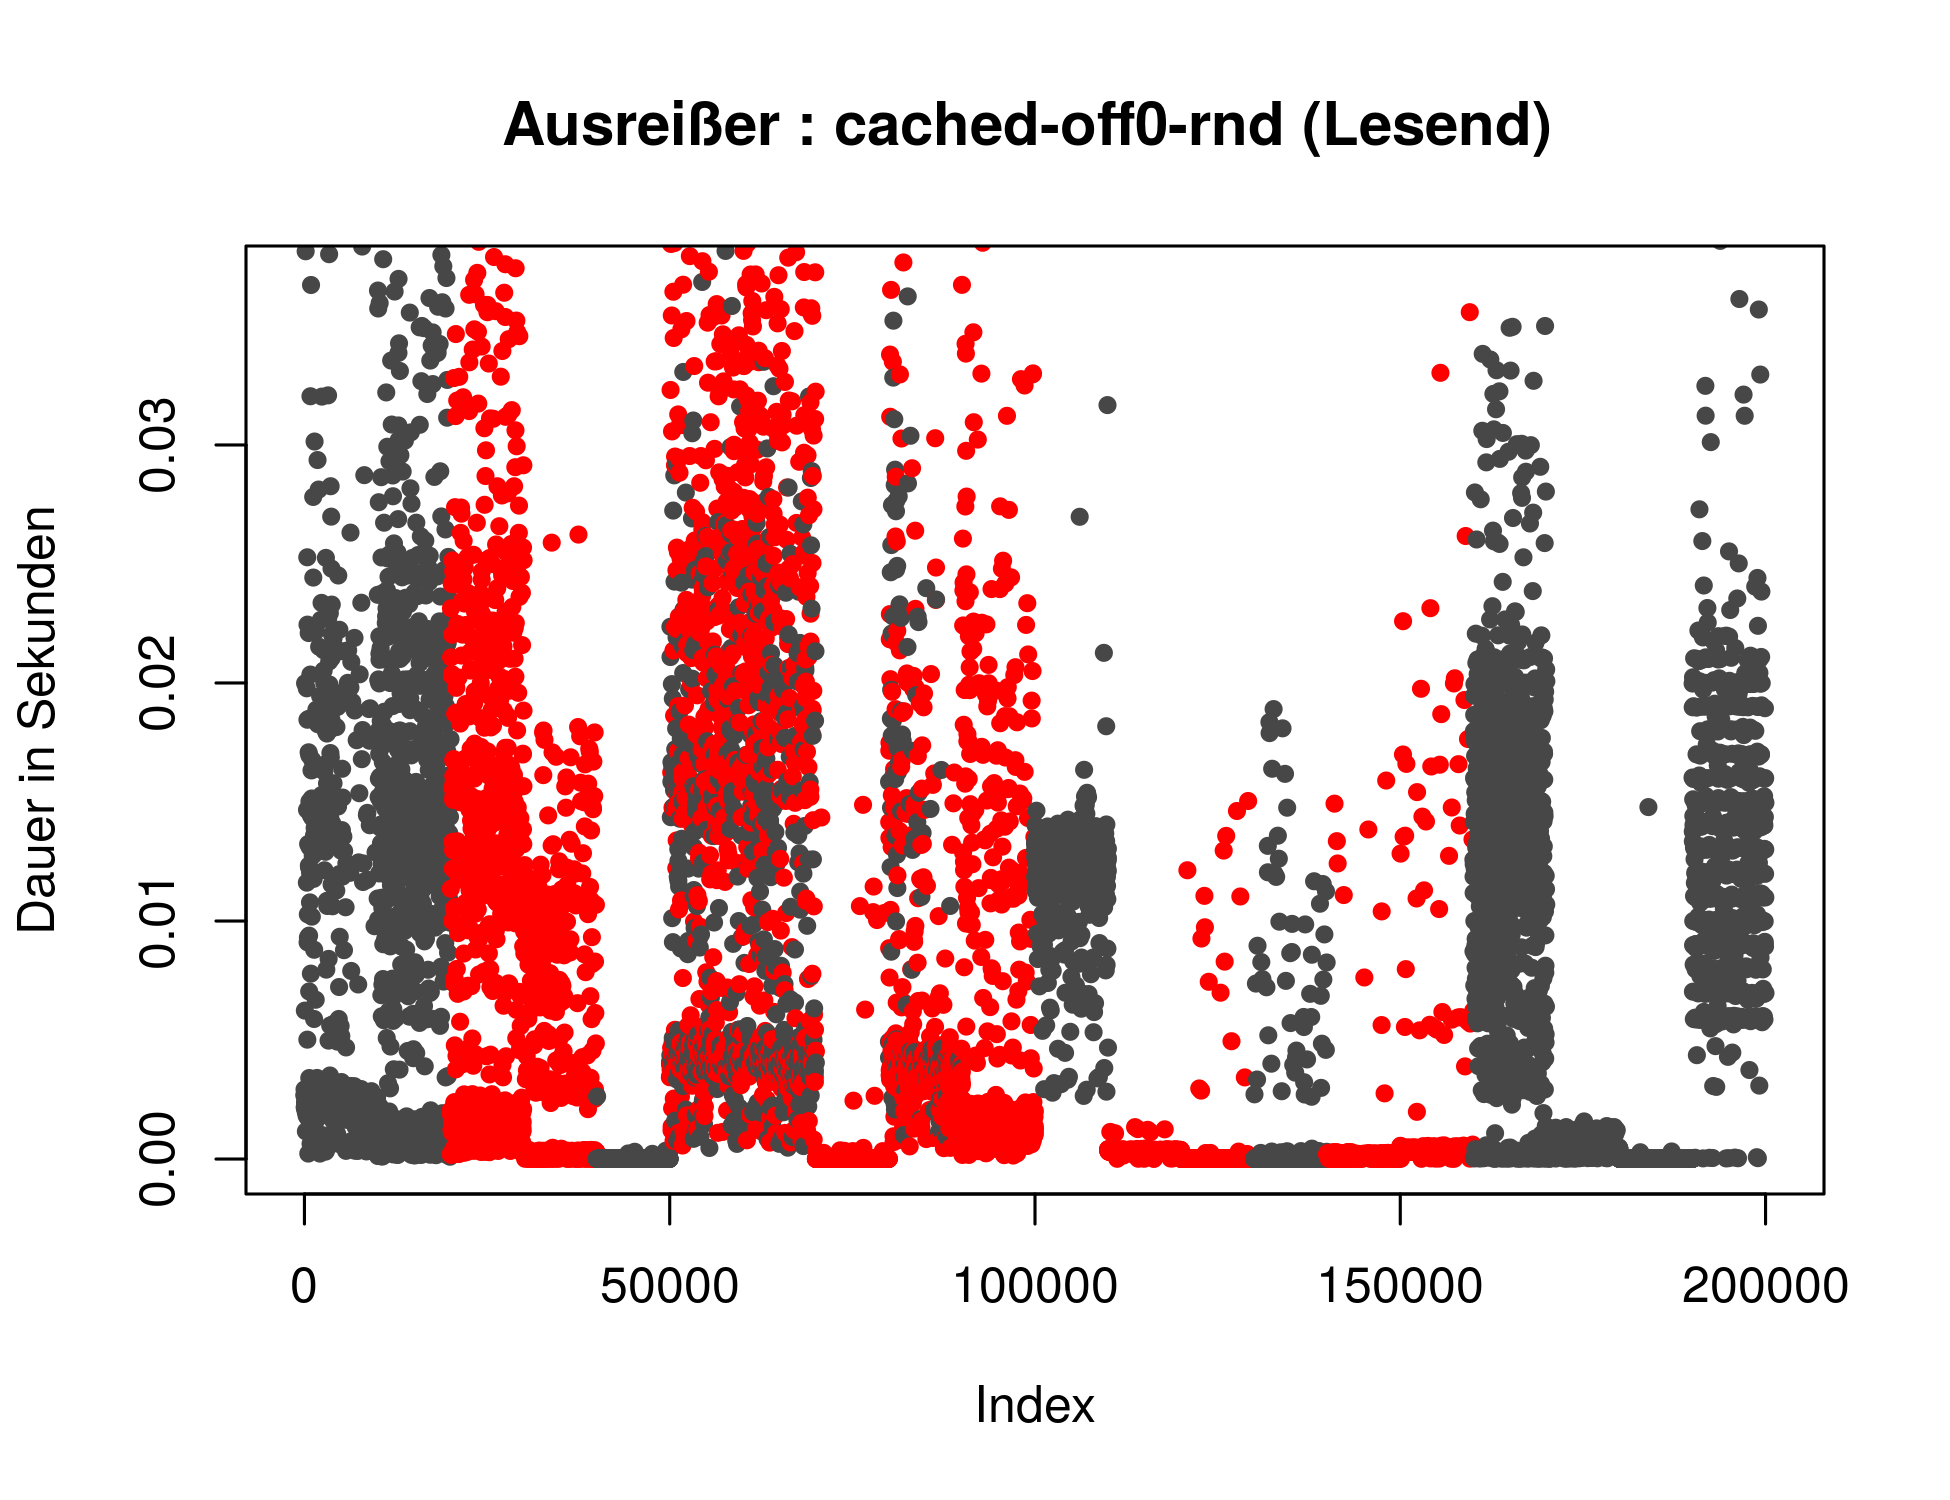
\includegraphics[width=.43\textwidth]{Bilder/Plots/exploration/plot_outlier_read_rnd.png}
	}
	\hfill
	\subfloat{
		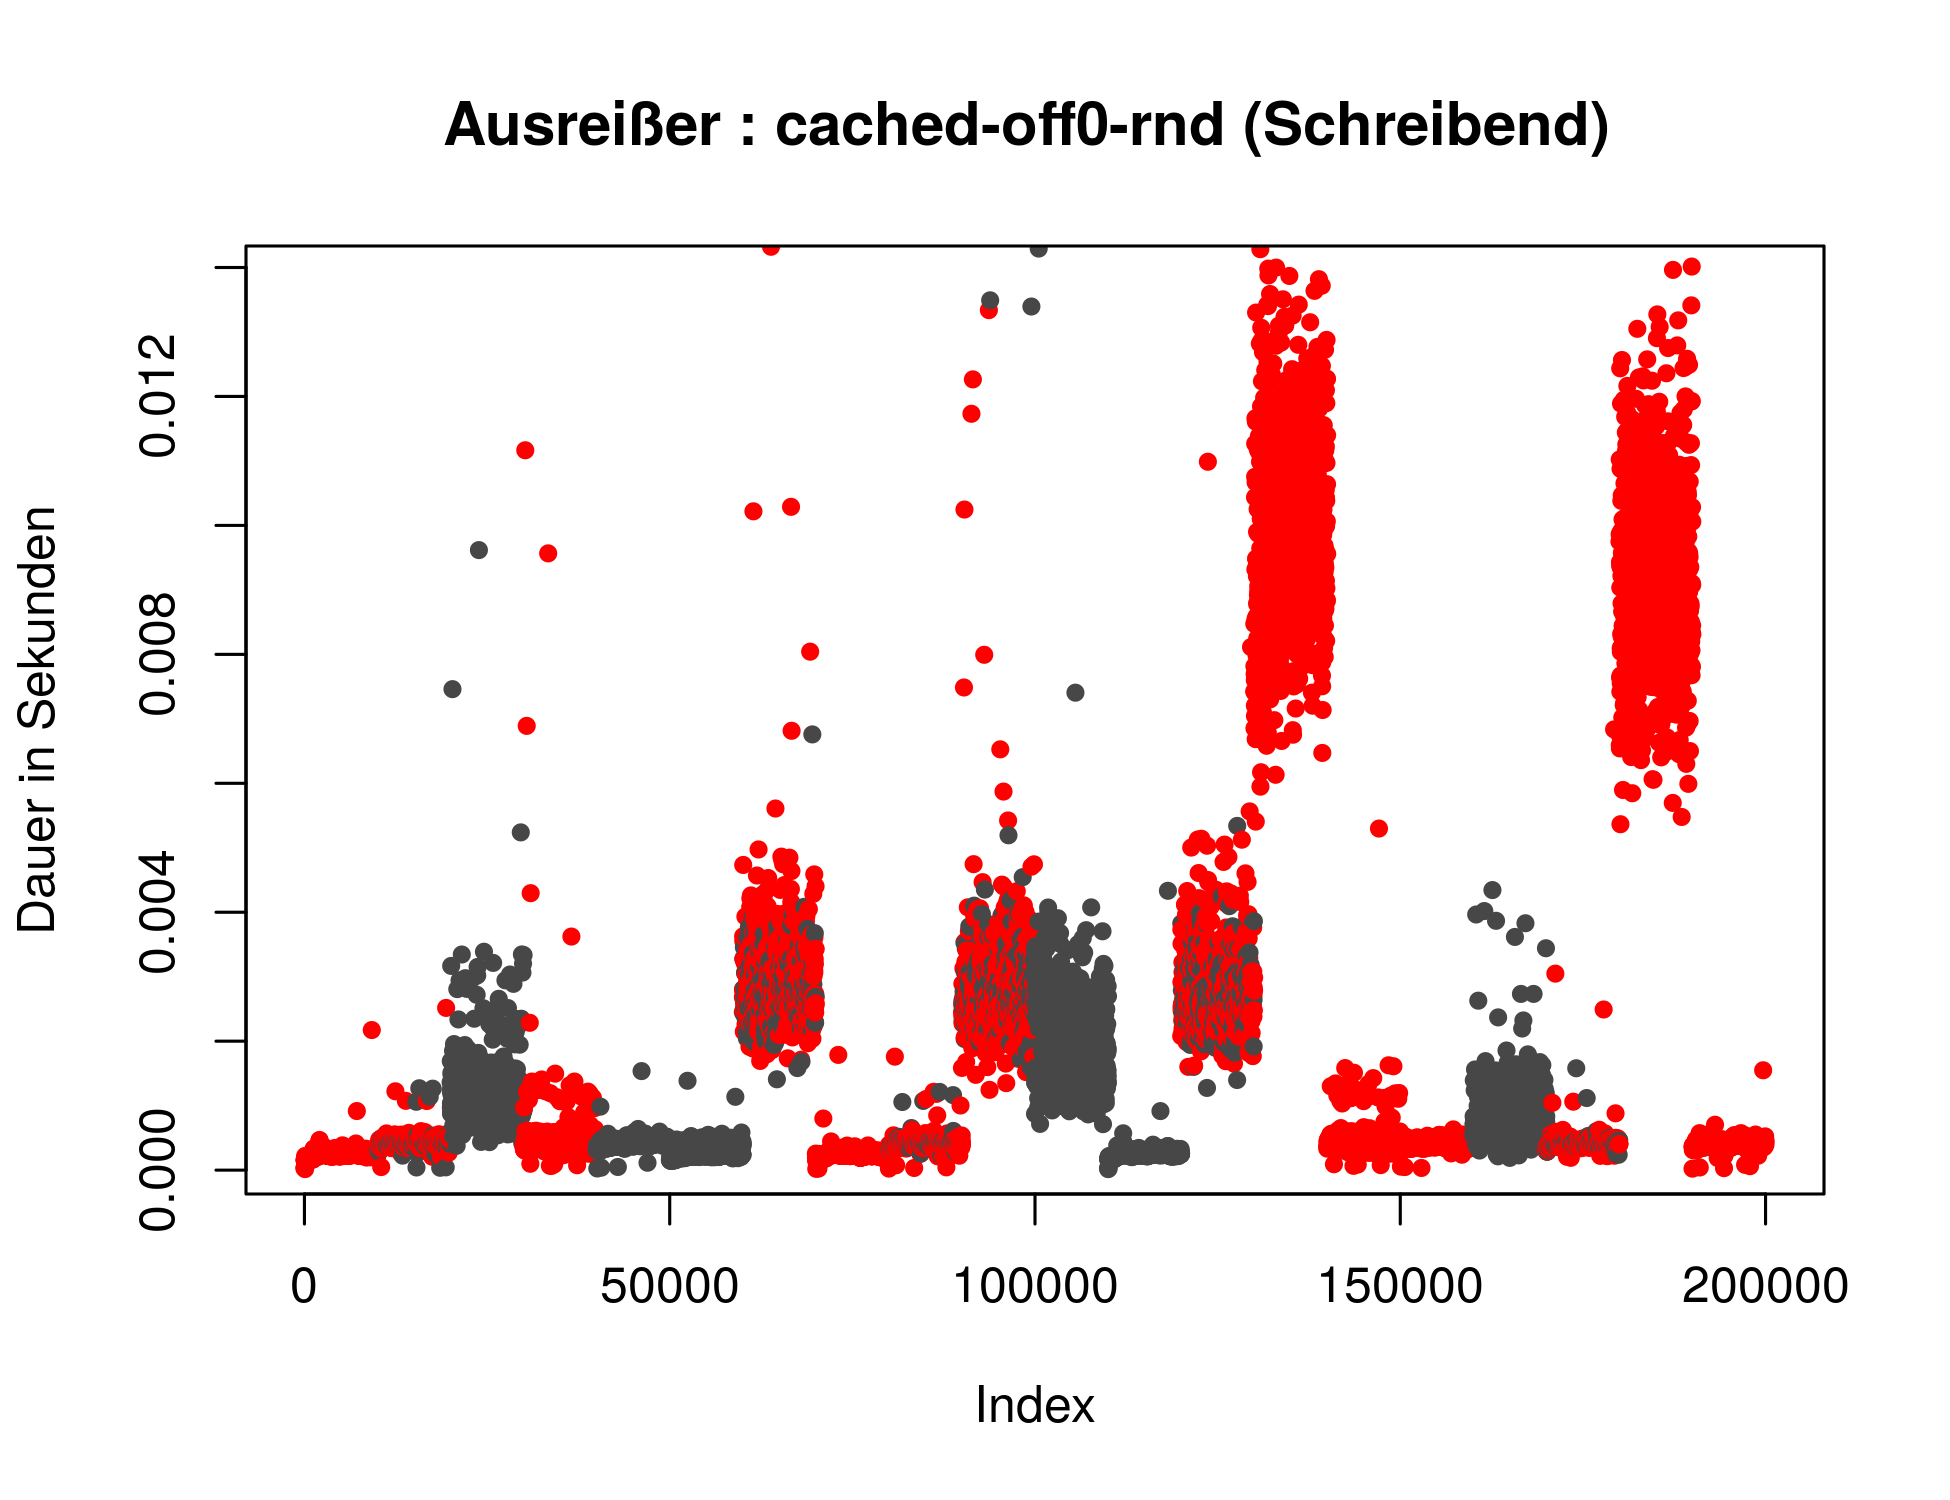
\includegraphics[width=.43\textwidth]{Bilder/Plots/exploration/plot_outlier_write_rnd.png}
	}		
	\caption{Ausreißer sind in rot dargstellt, sie überdecken die grauen Punkte}
	\label{fig:ausreisser}
\end{figure} 

Bei der Betrachtung der Metainformationen wurde festgestellt, dass die Zugriffsgröße sehr stark mit der Laufzeit eines Messpunktes korreliert. Um eine Vorstellung davon zu entwickeln, wie diese beiden Größen miteinander zusammenhängen, habe ich die Messdaten nach der Zugriffsgröße sortiert und ihre Laufzeit aufgetragen. \ref{fig:Zugriffsgroesse_Sortiert} \\
Die Korrelation der beiden Größen ist deutlich erkennbar, die Laufzeiten nehmen im Mittel zu. Doch es ist auch zu erkennen, insbesondere bei cached-off0-rnd-R, dass die Laufzeiten aufgrund der Streuung von weiteren Faktoren abhängen müssen. Die Verteilung der Messpunkte einer Zugriffsgröße in zwei bis drei deutlich zu unterscheidende Gruppen deutete darauf hin, dass Messungen innerhalb einer vom E/A-System Gruppe ähnlich behandelt wurden.

\begin{figure}
	\subfloat[Von links nach rechts in KB: 1, 4, 16, 256, 1024, 16384, 65536, 262144, 524288, 1048576, 2097152, 4194304, 8388608, 16777216]{
		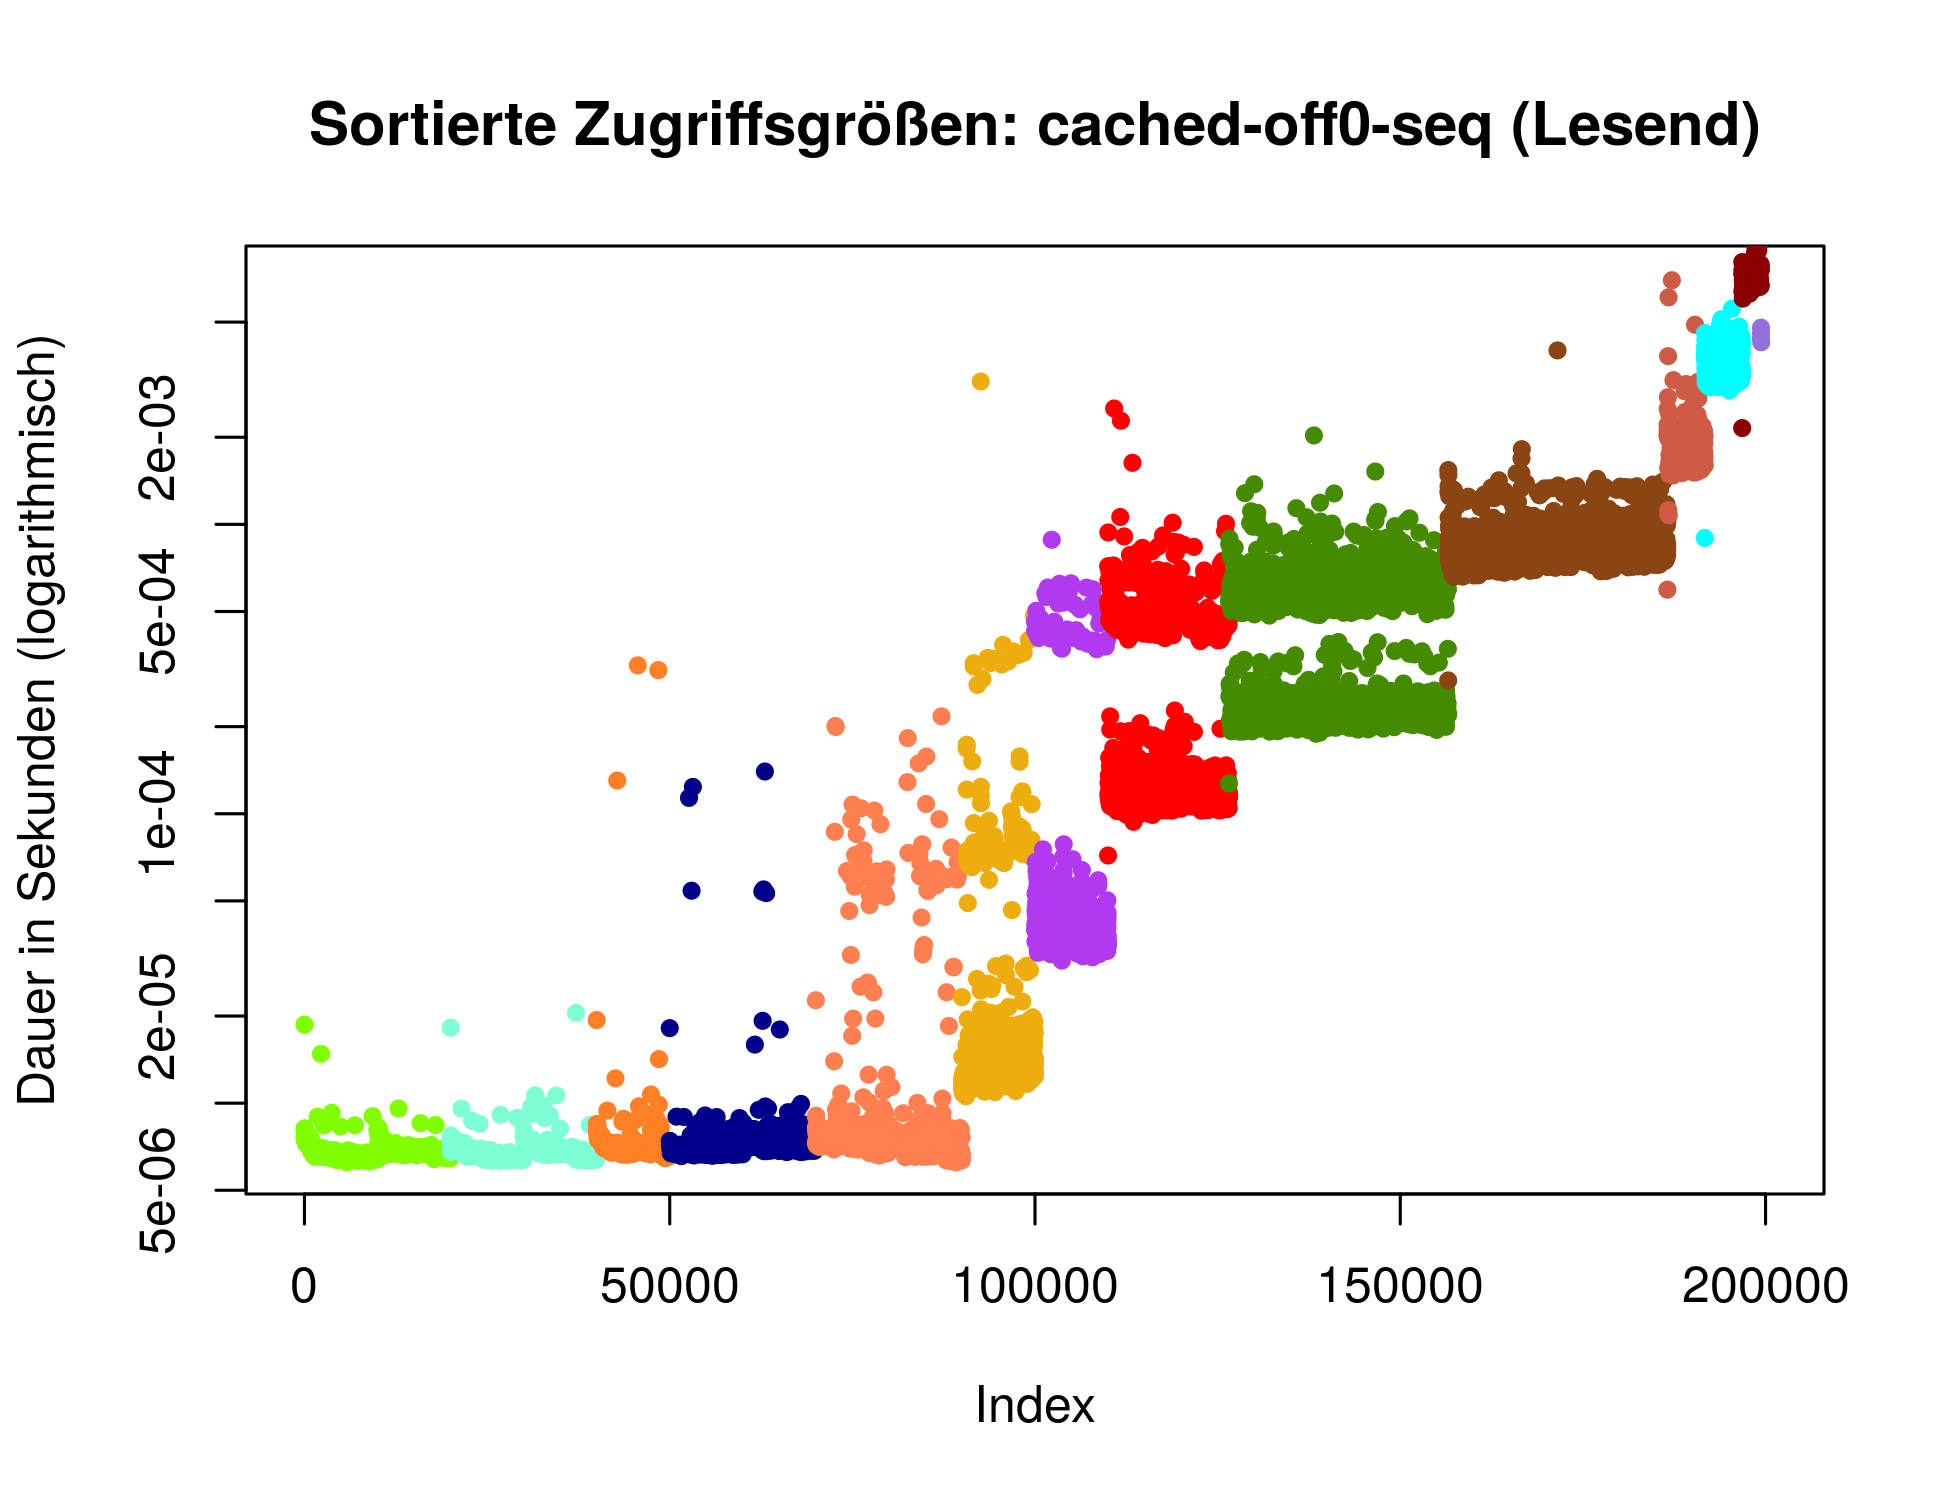
\includegraphics[width=.5\textwidth]{Bilder/Plots/exploration/plot_SizeSorted_read_seq.png}
	}
	\hfill
	\subfloat[Von links nach rechts in KB: 1, 4, 16, 64, 256, 1024, 4096, 8192, 16384, 65536, 262144, 524288, 2097152, 4194304, 16777216]{
		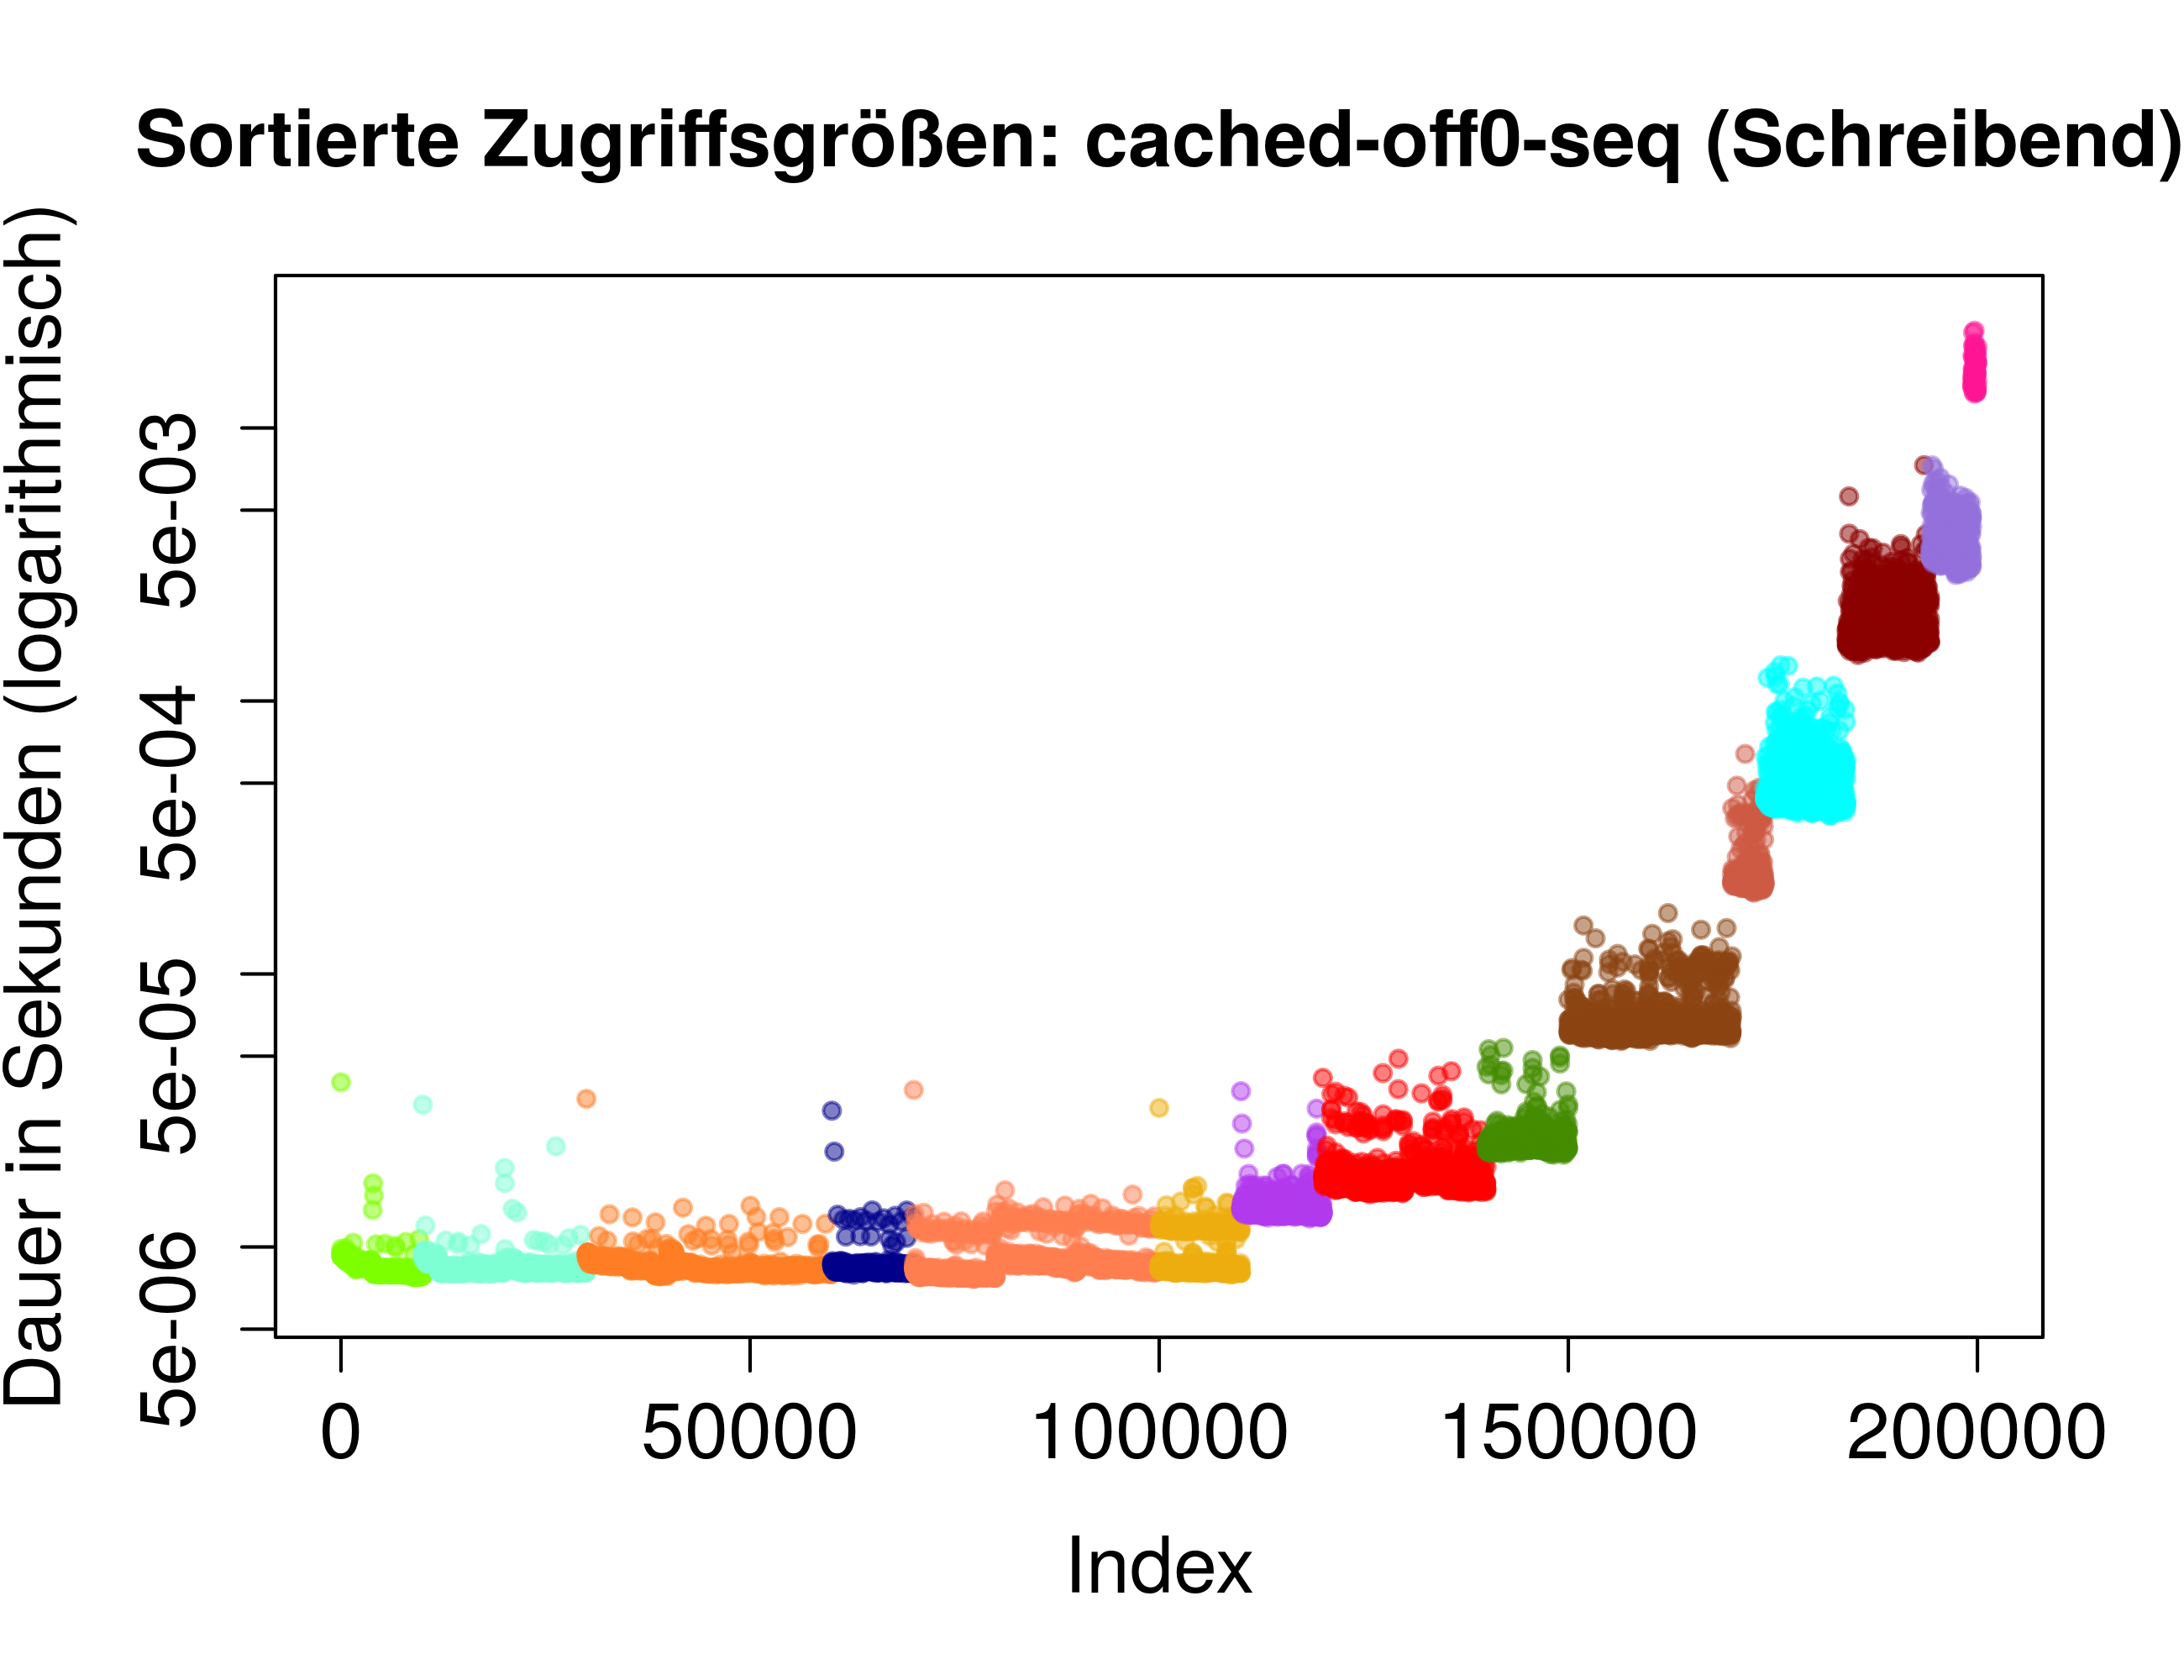
\includegraphics[width=.5\textwidth]{Bilder/Plots/exploration/plot_SizeSorted_write_seq.png}
	}\\
	\subfloat[Von links nach rechts in KB: 1, 4, 16, 64, 256, 4096, 8192, 16384, 65536, 262144, 524288, 1048576, 2097152, 8388608]{
		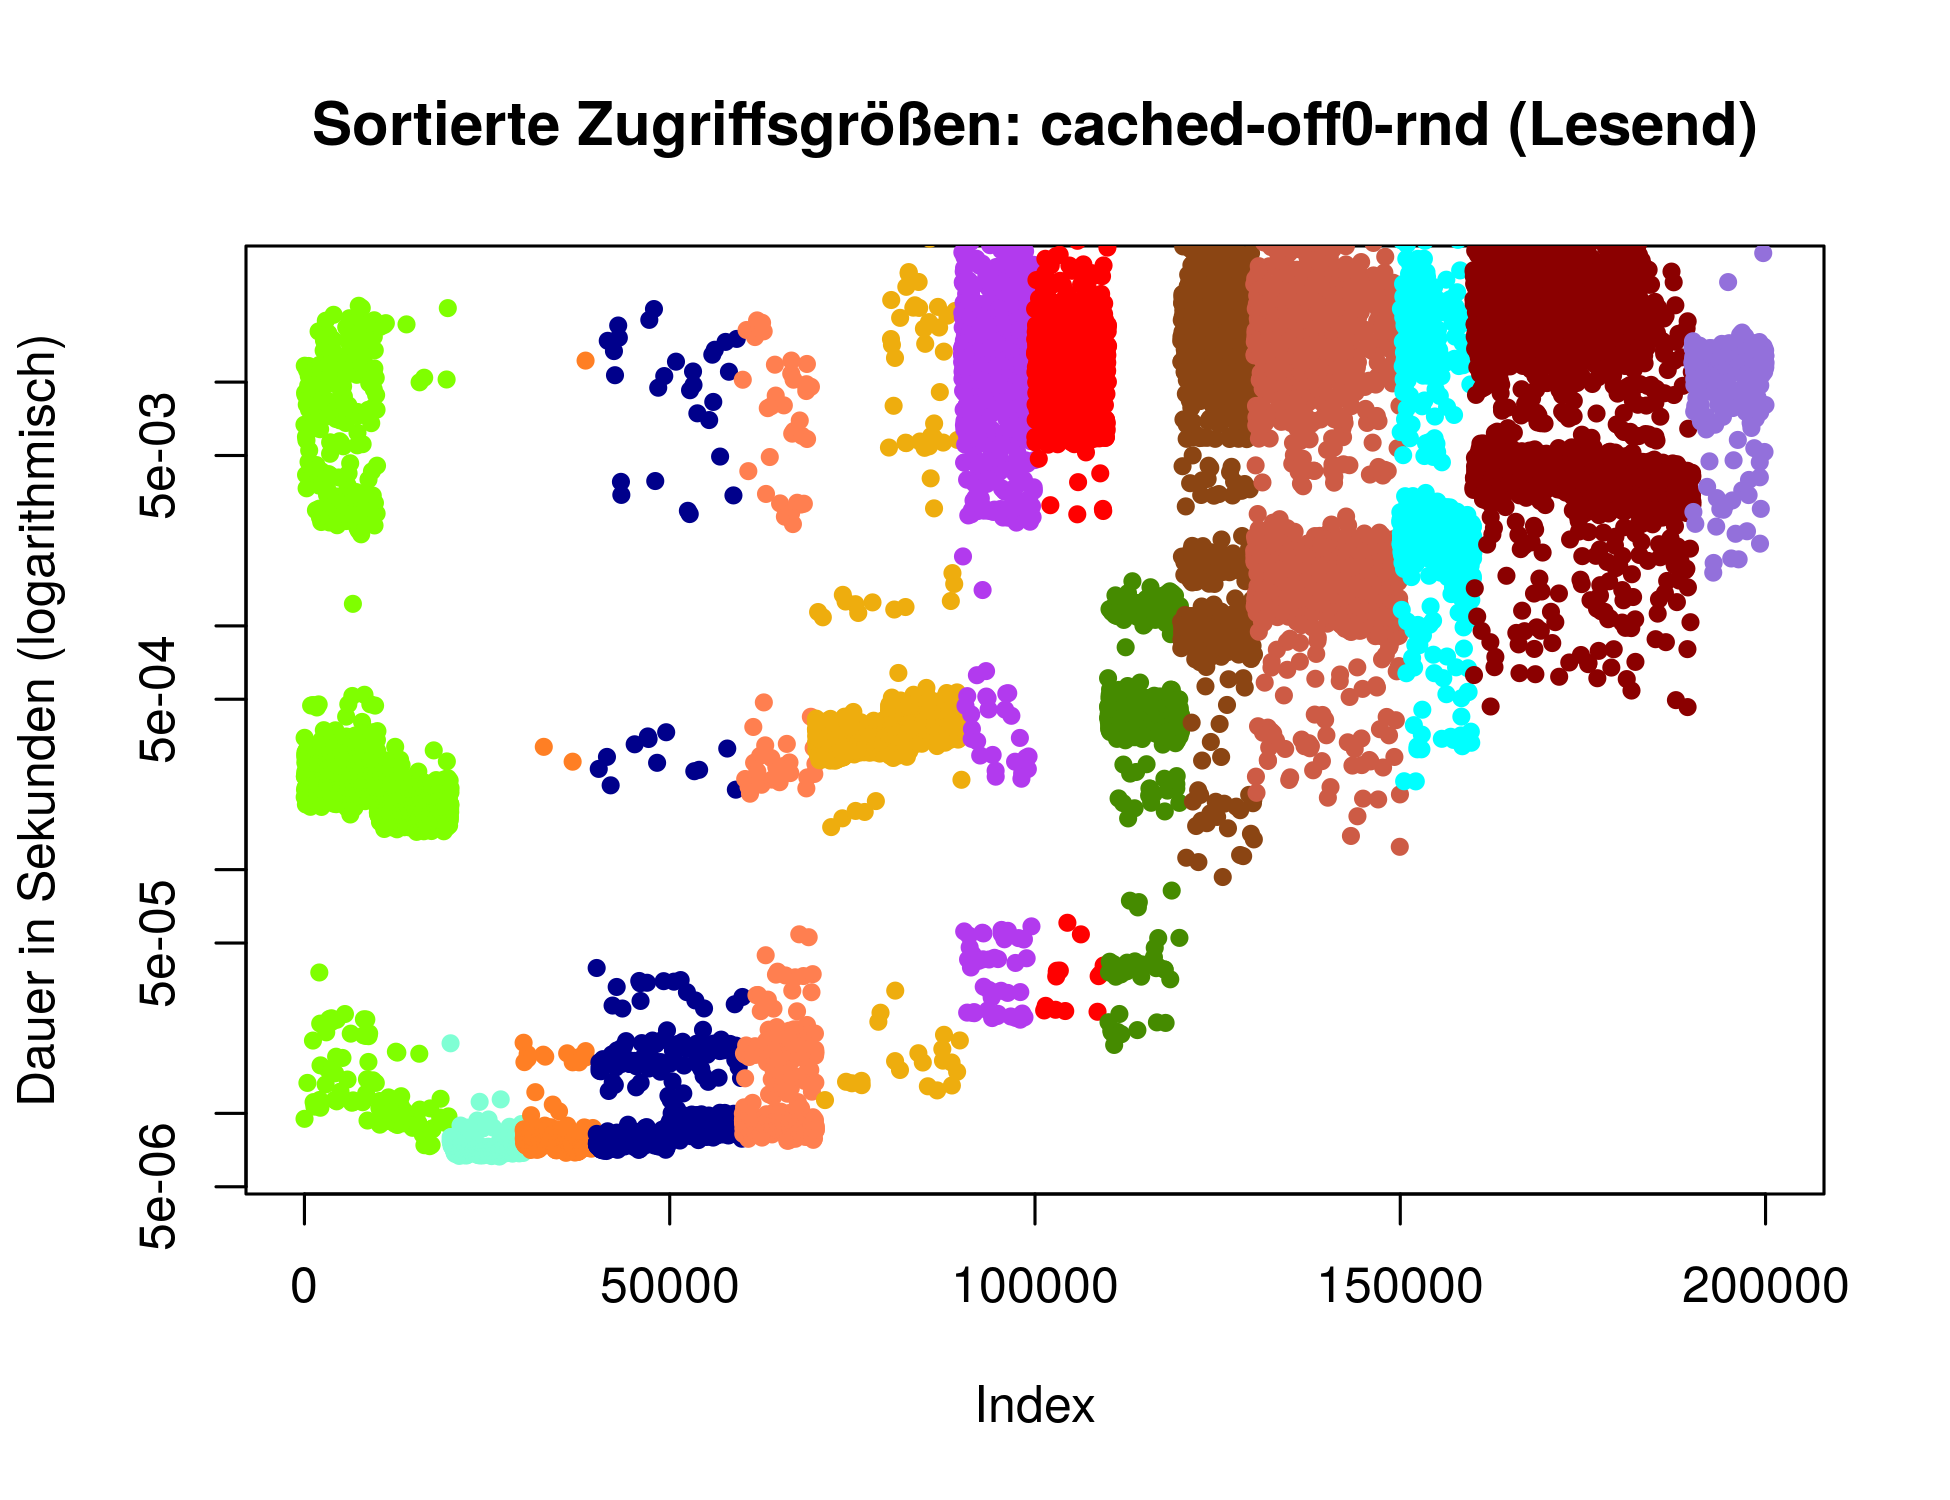
\includegraphics[width=.5\textwidth]{Bilder/Plots/exploration/plot_SizeSorted_read_rnd.png}
	}
	\hfill
	\subfloat[Von links nach rechts in KB: 1, 4, 1024, 4096, 8192, 16384, 65536, 262144, 524288, 1048576, 2097152, 8388608]{
		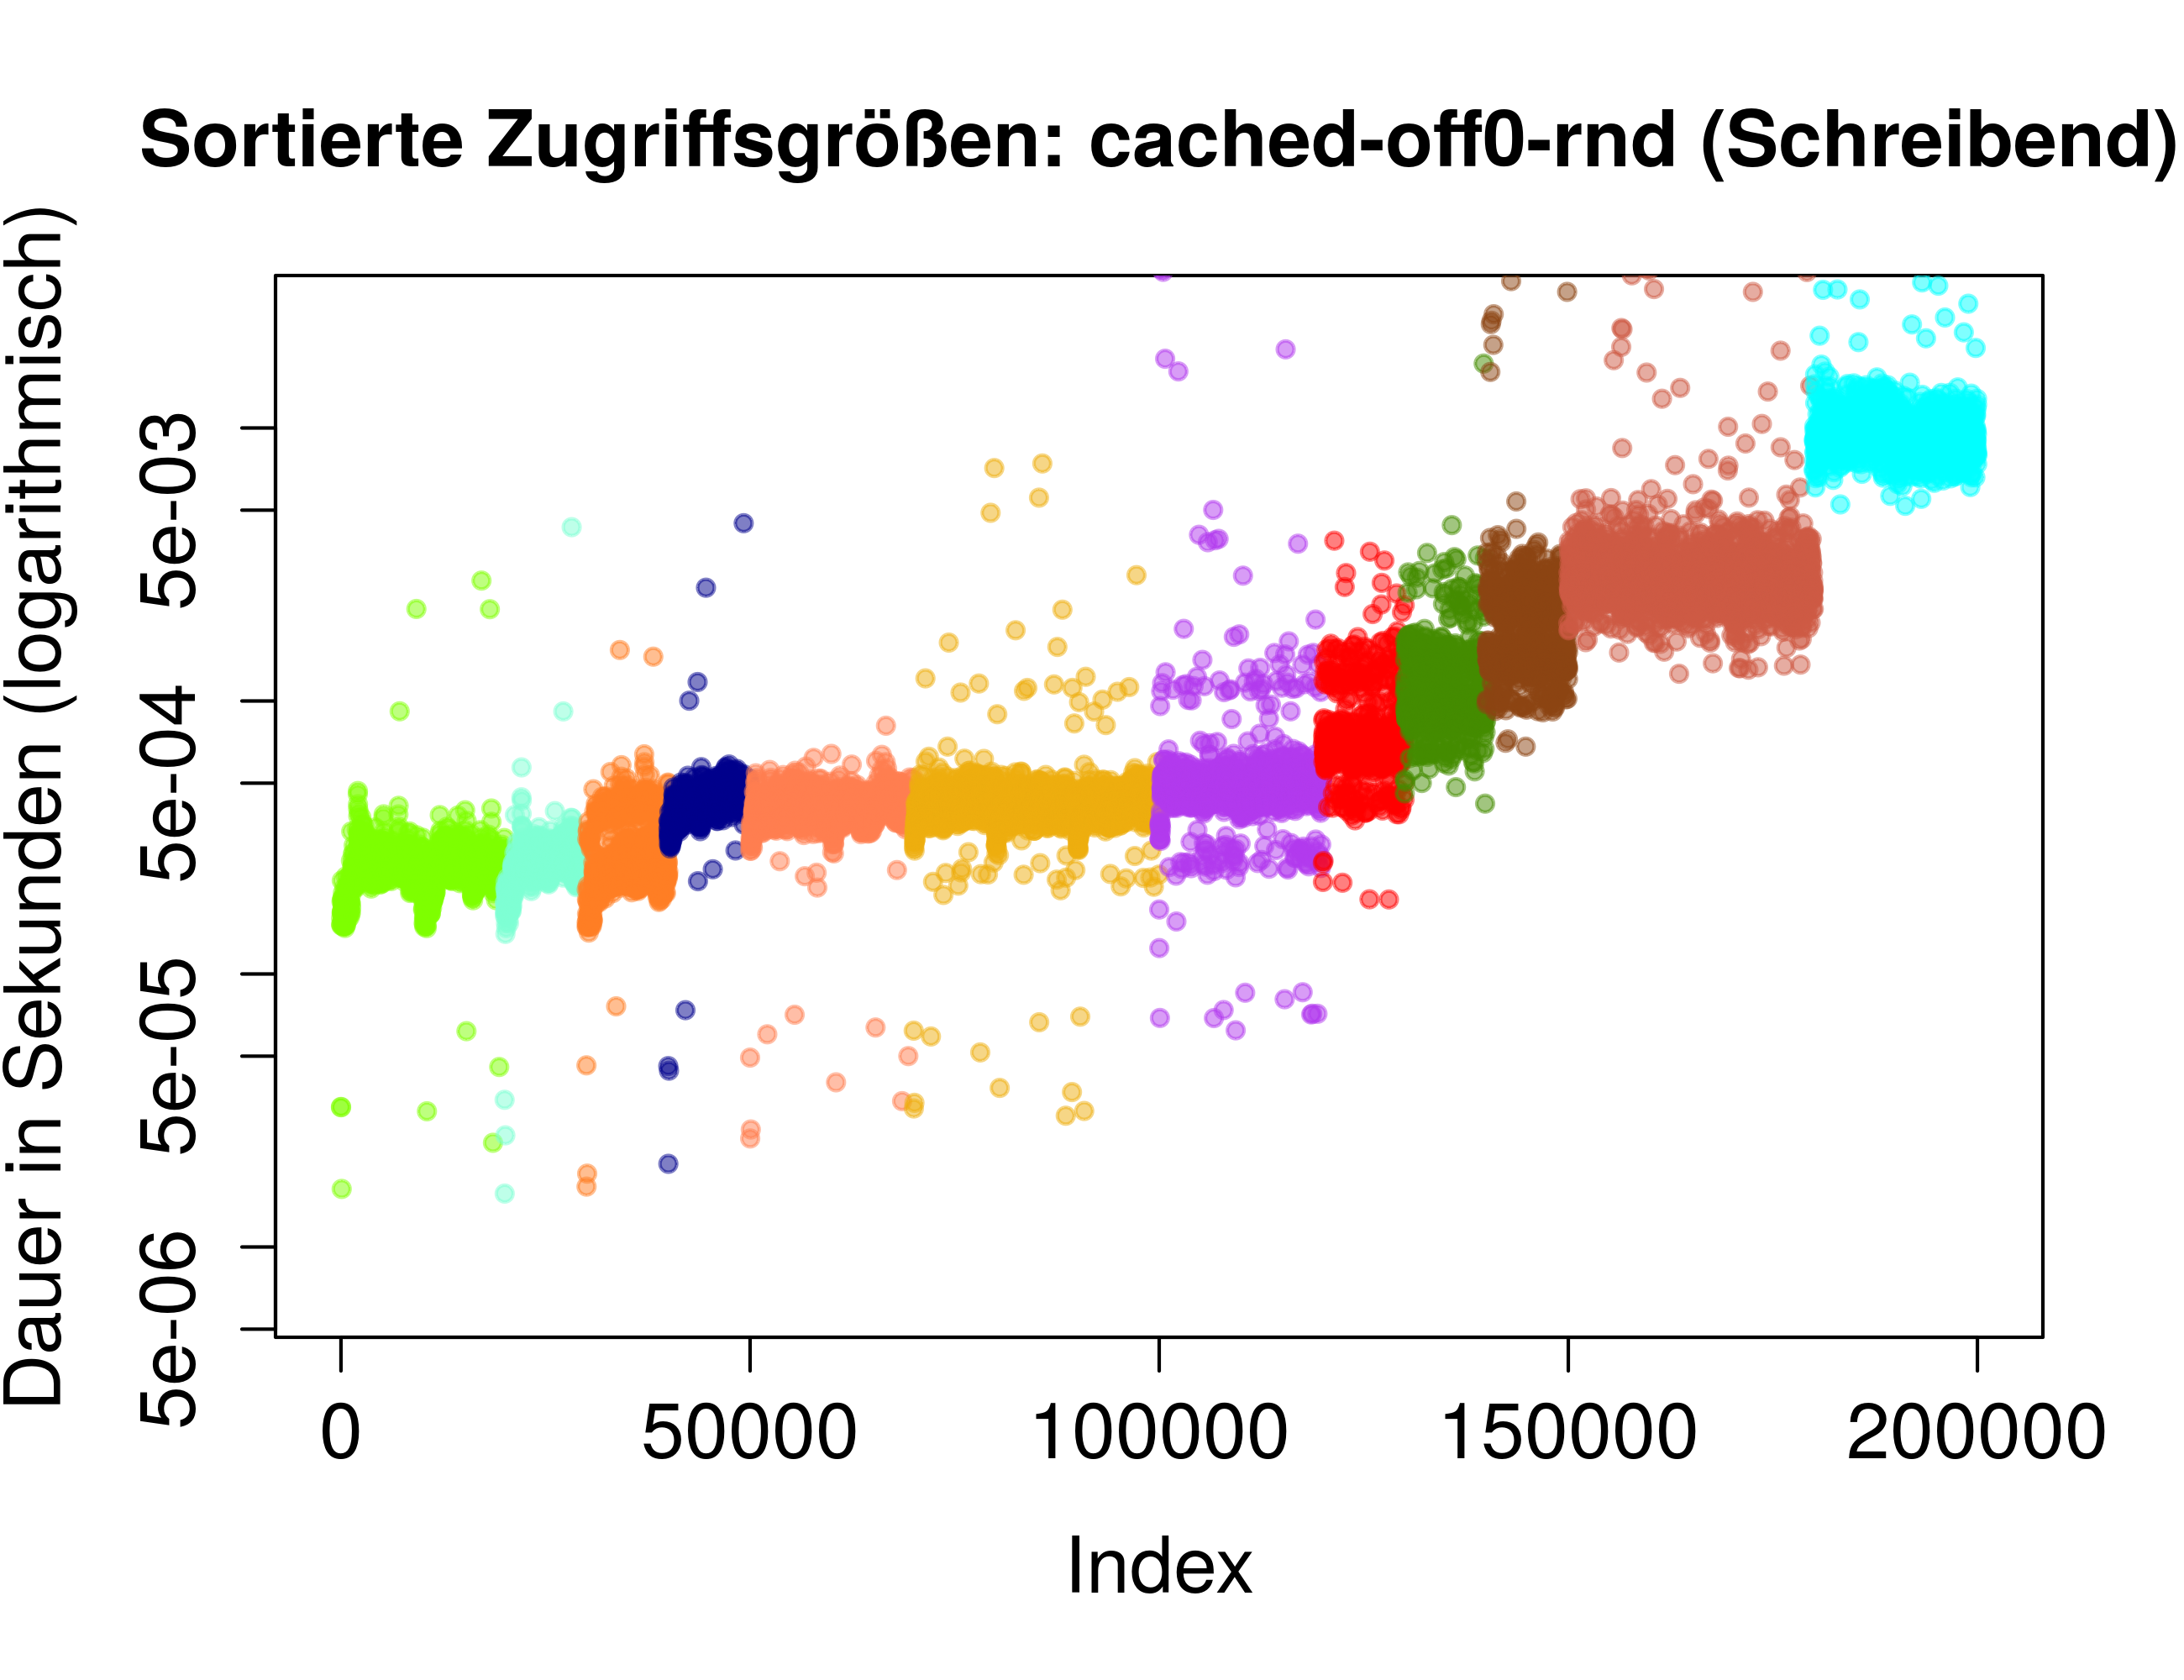
\includegraphics[width=.5\textwidth]{Bilder/Plots/exploration/plot_SizeSorted_write_rnd.png}
	}		
	\caption{Messungen der Laufzeiten nach Zugriffsgröße sortiert dargestellt (logarithmische Y-Achse)}
	\label{fig:Zugriffsgroesse_Sortiert}
\end{figure} 

Um die unterschiedlichen Laufzeiten innerhalb einer Zugriffsgröße zu untersuchen, habe ich für die Größen 1KB, 16384KB und 2097152KB (diese Zugriffsgrößen kommen in allen vier Datensätzen vor) alle Messungen betrachtet.

\begin{figure}
	\subfloat{
		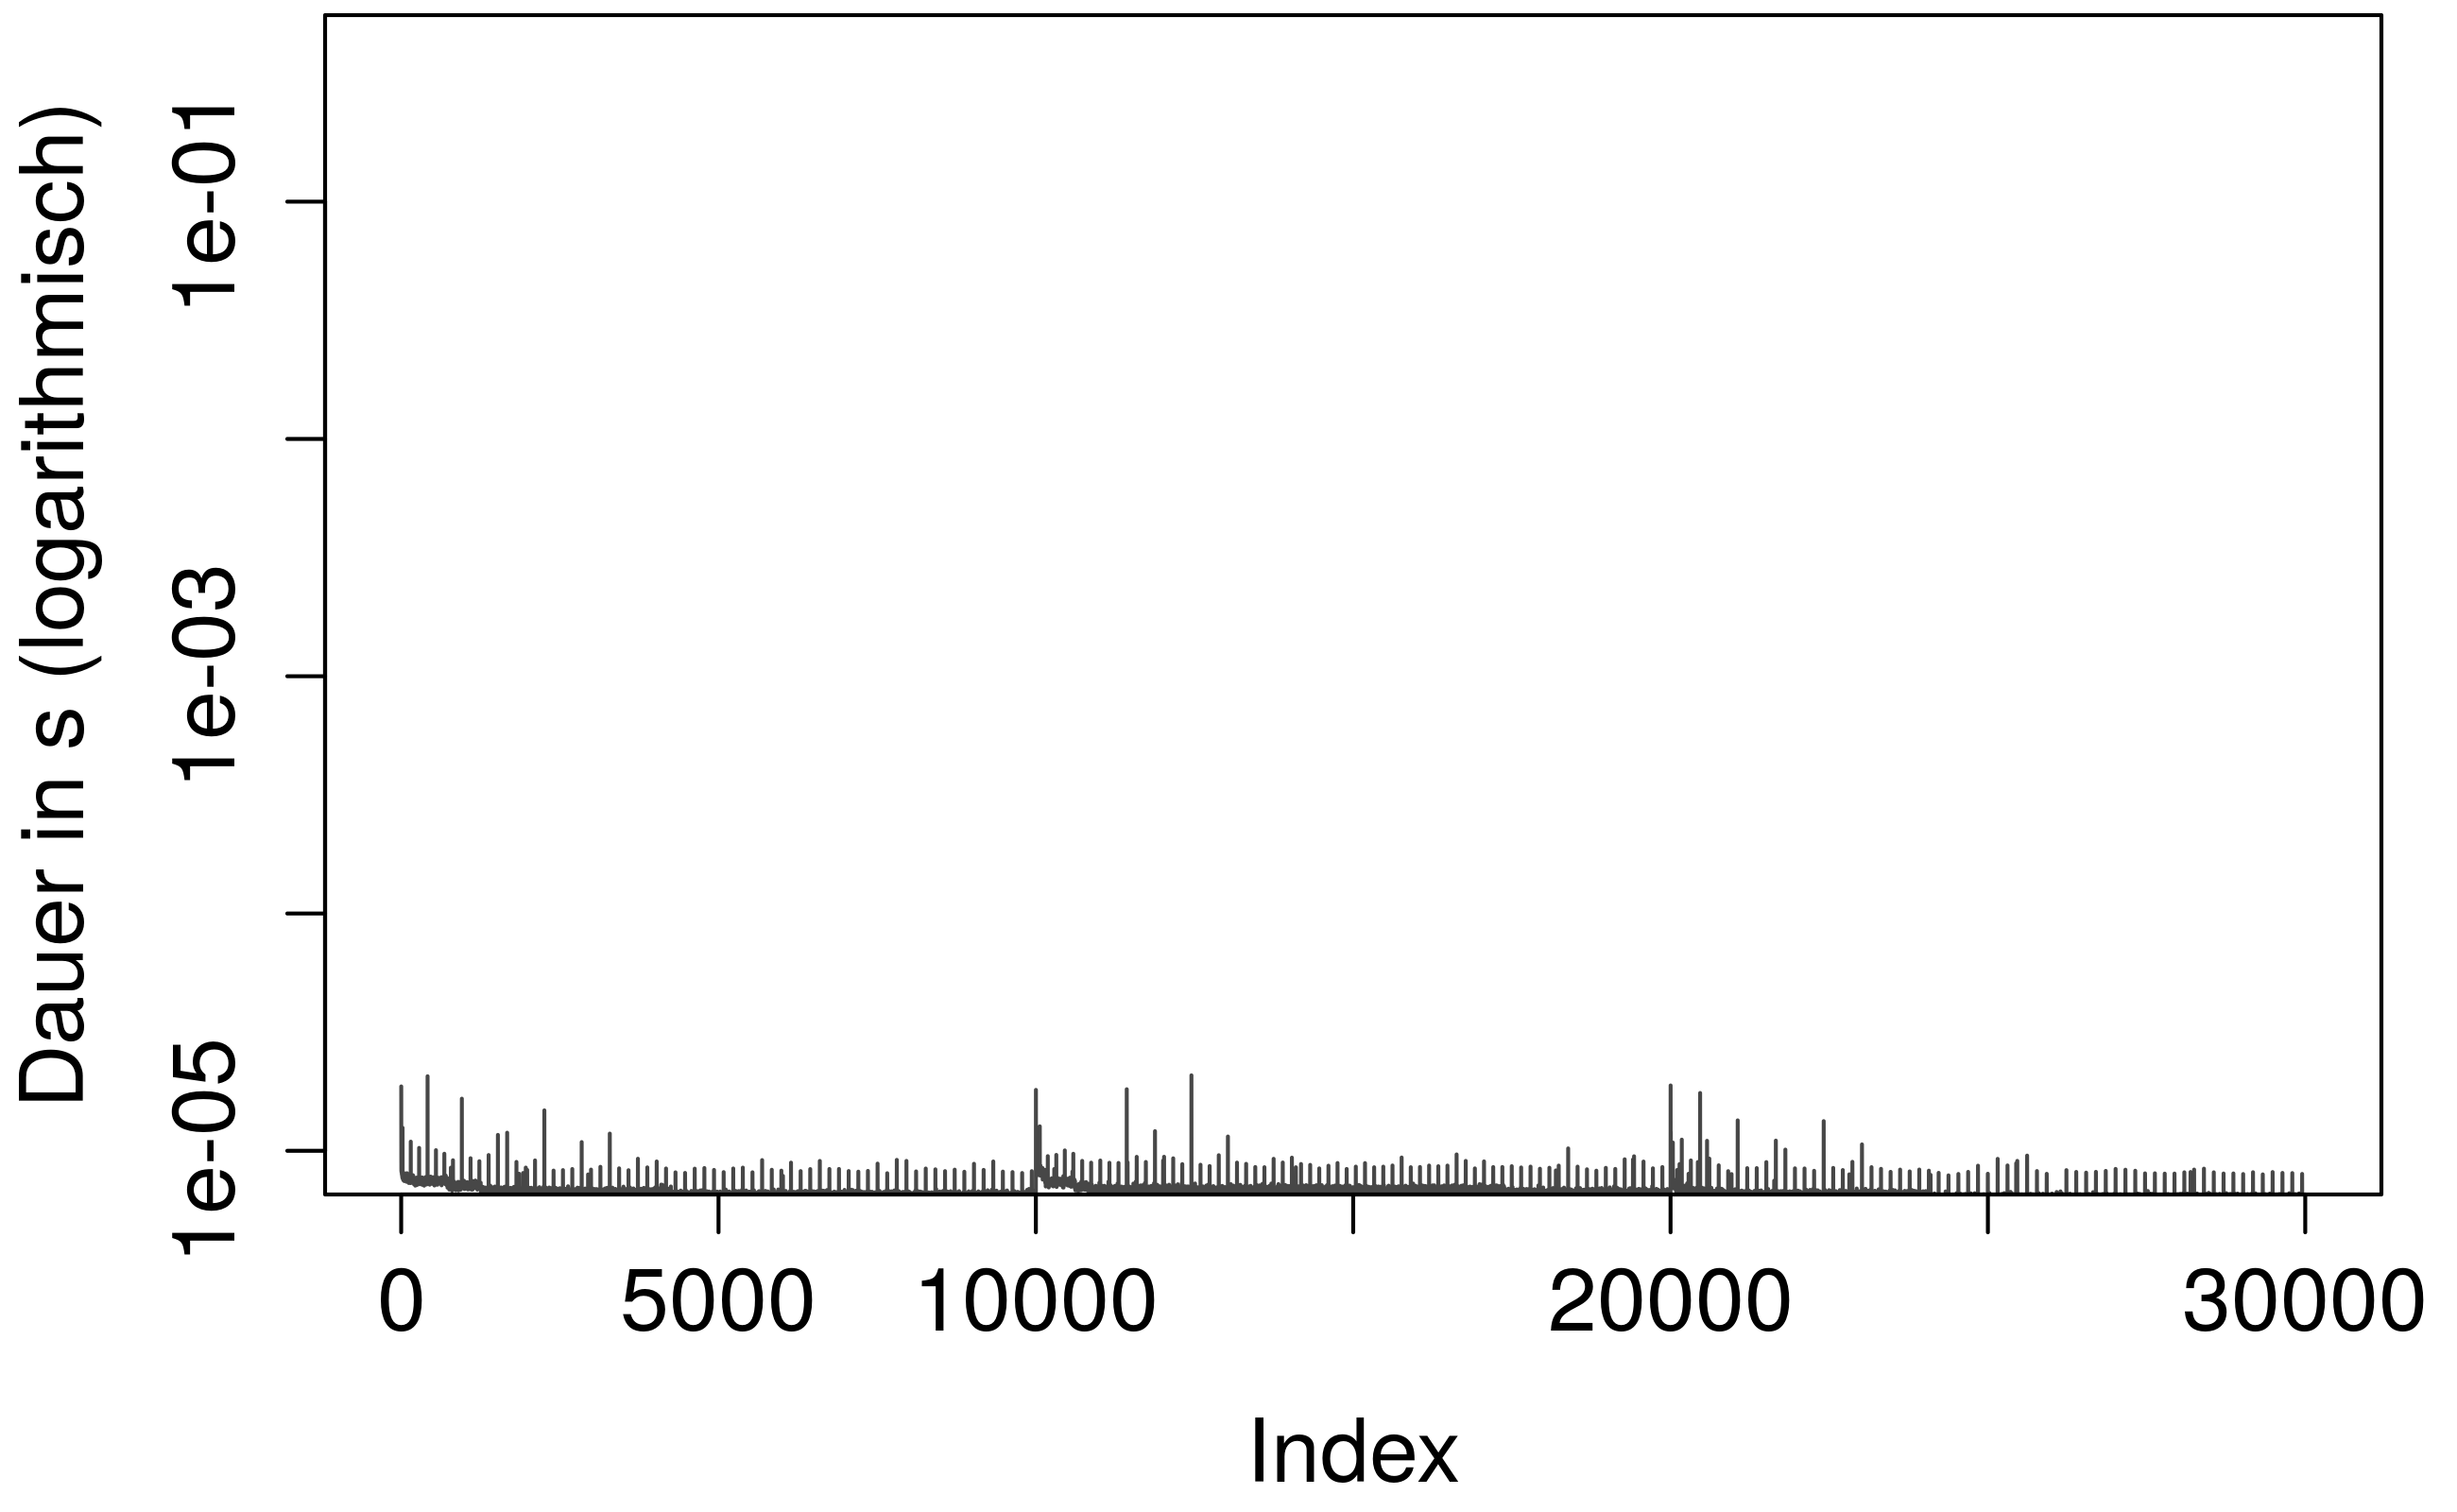
\includegraphics[width=.43\textwidth]{Bilder/Plots/exploration/plot_Size1_read_seq.png}
	}
	\hfill
	\subfloat{
		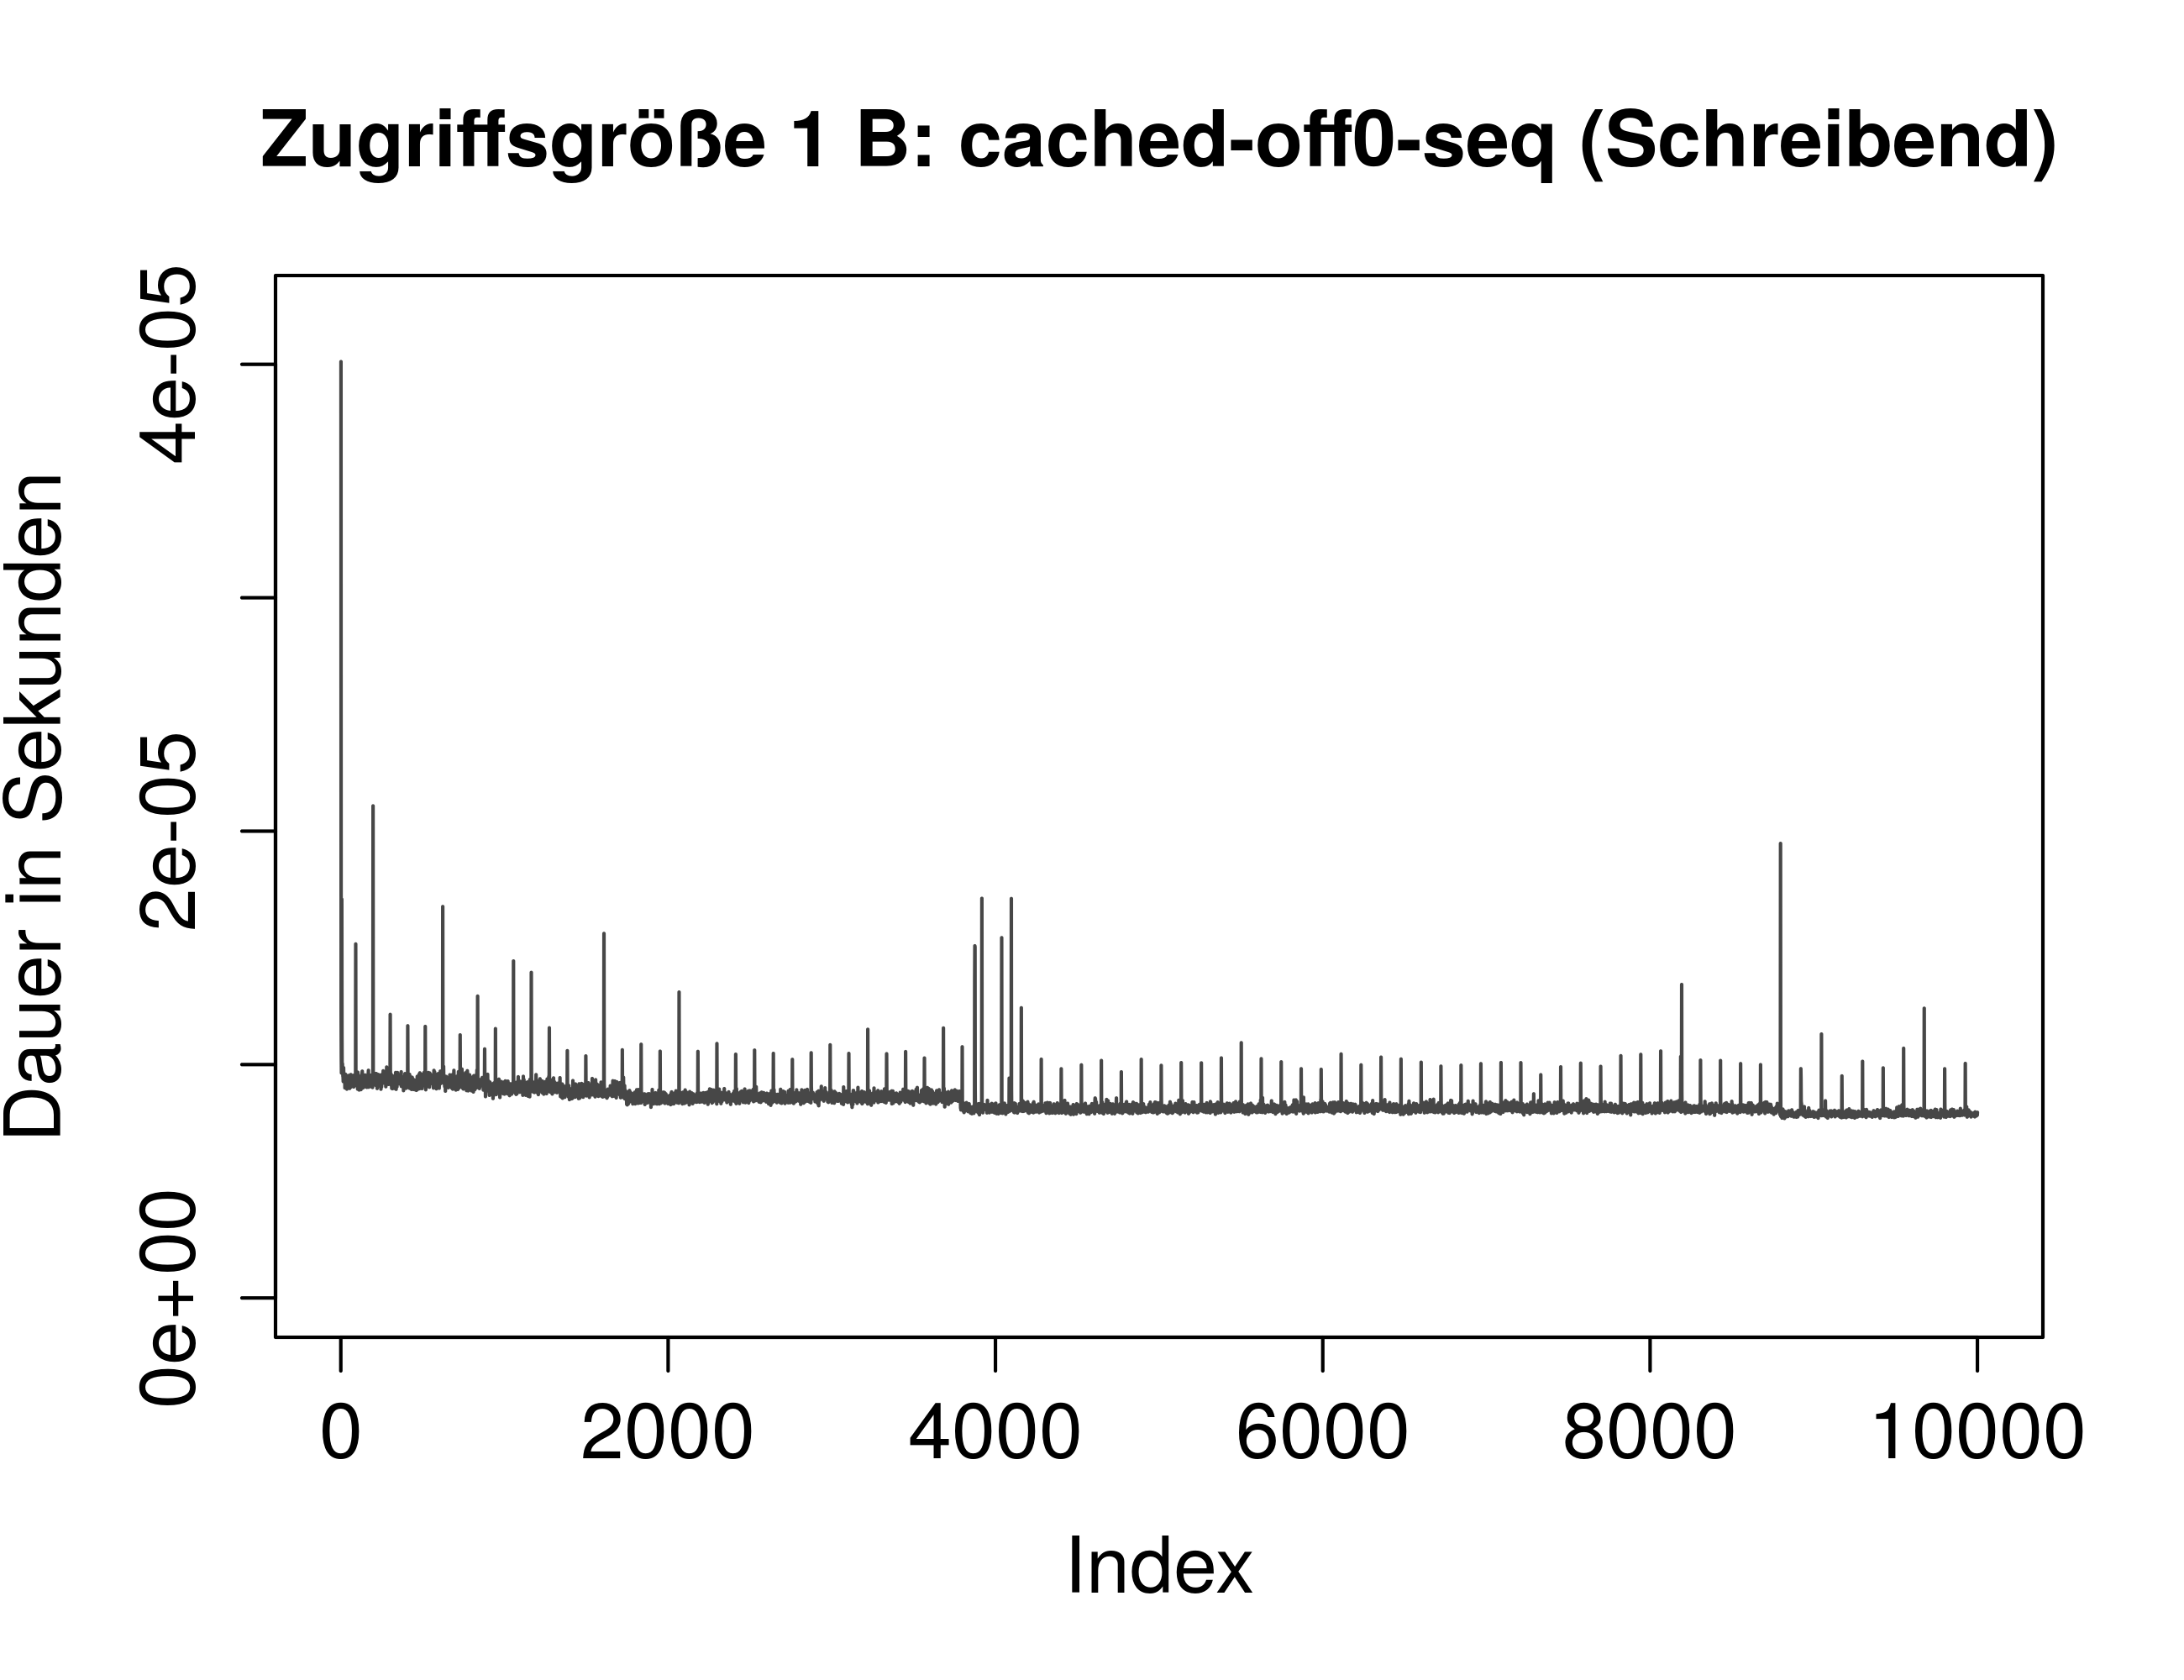
\includegraphics[width=.43\textwidth]{Bilder/Plots/exploration/plot_Size1_write_seq.png}
	}\\
	\subfloat{
		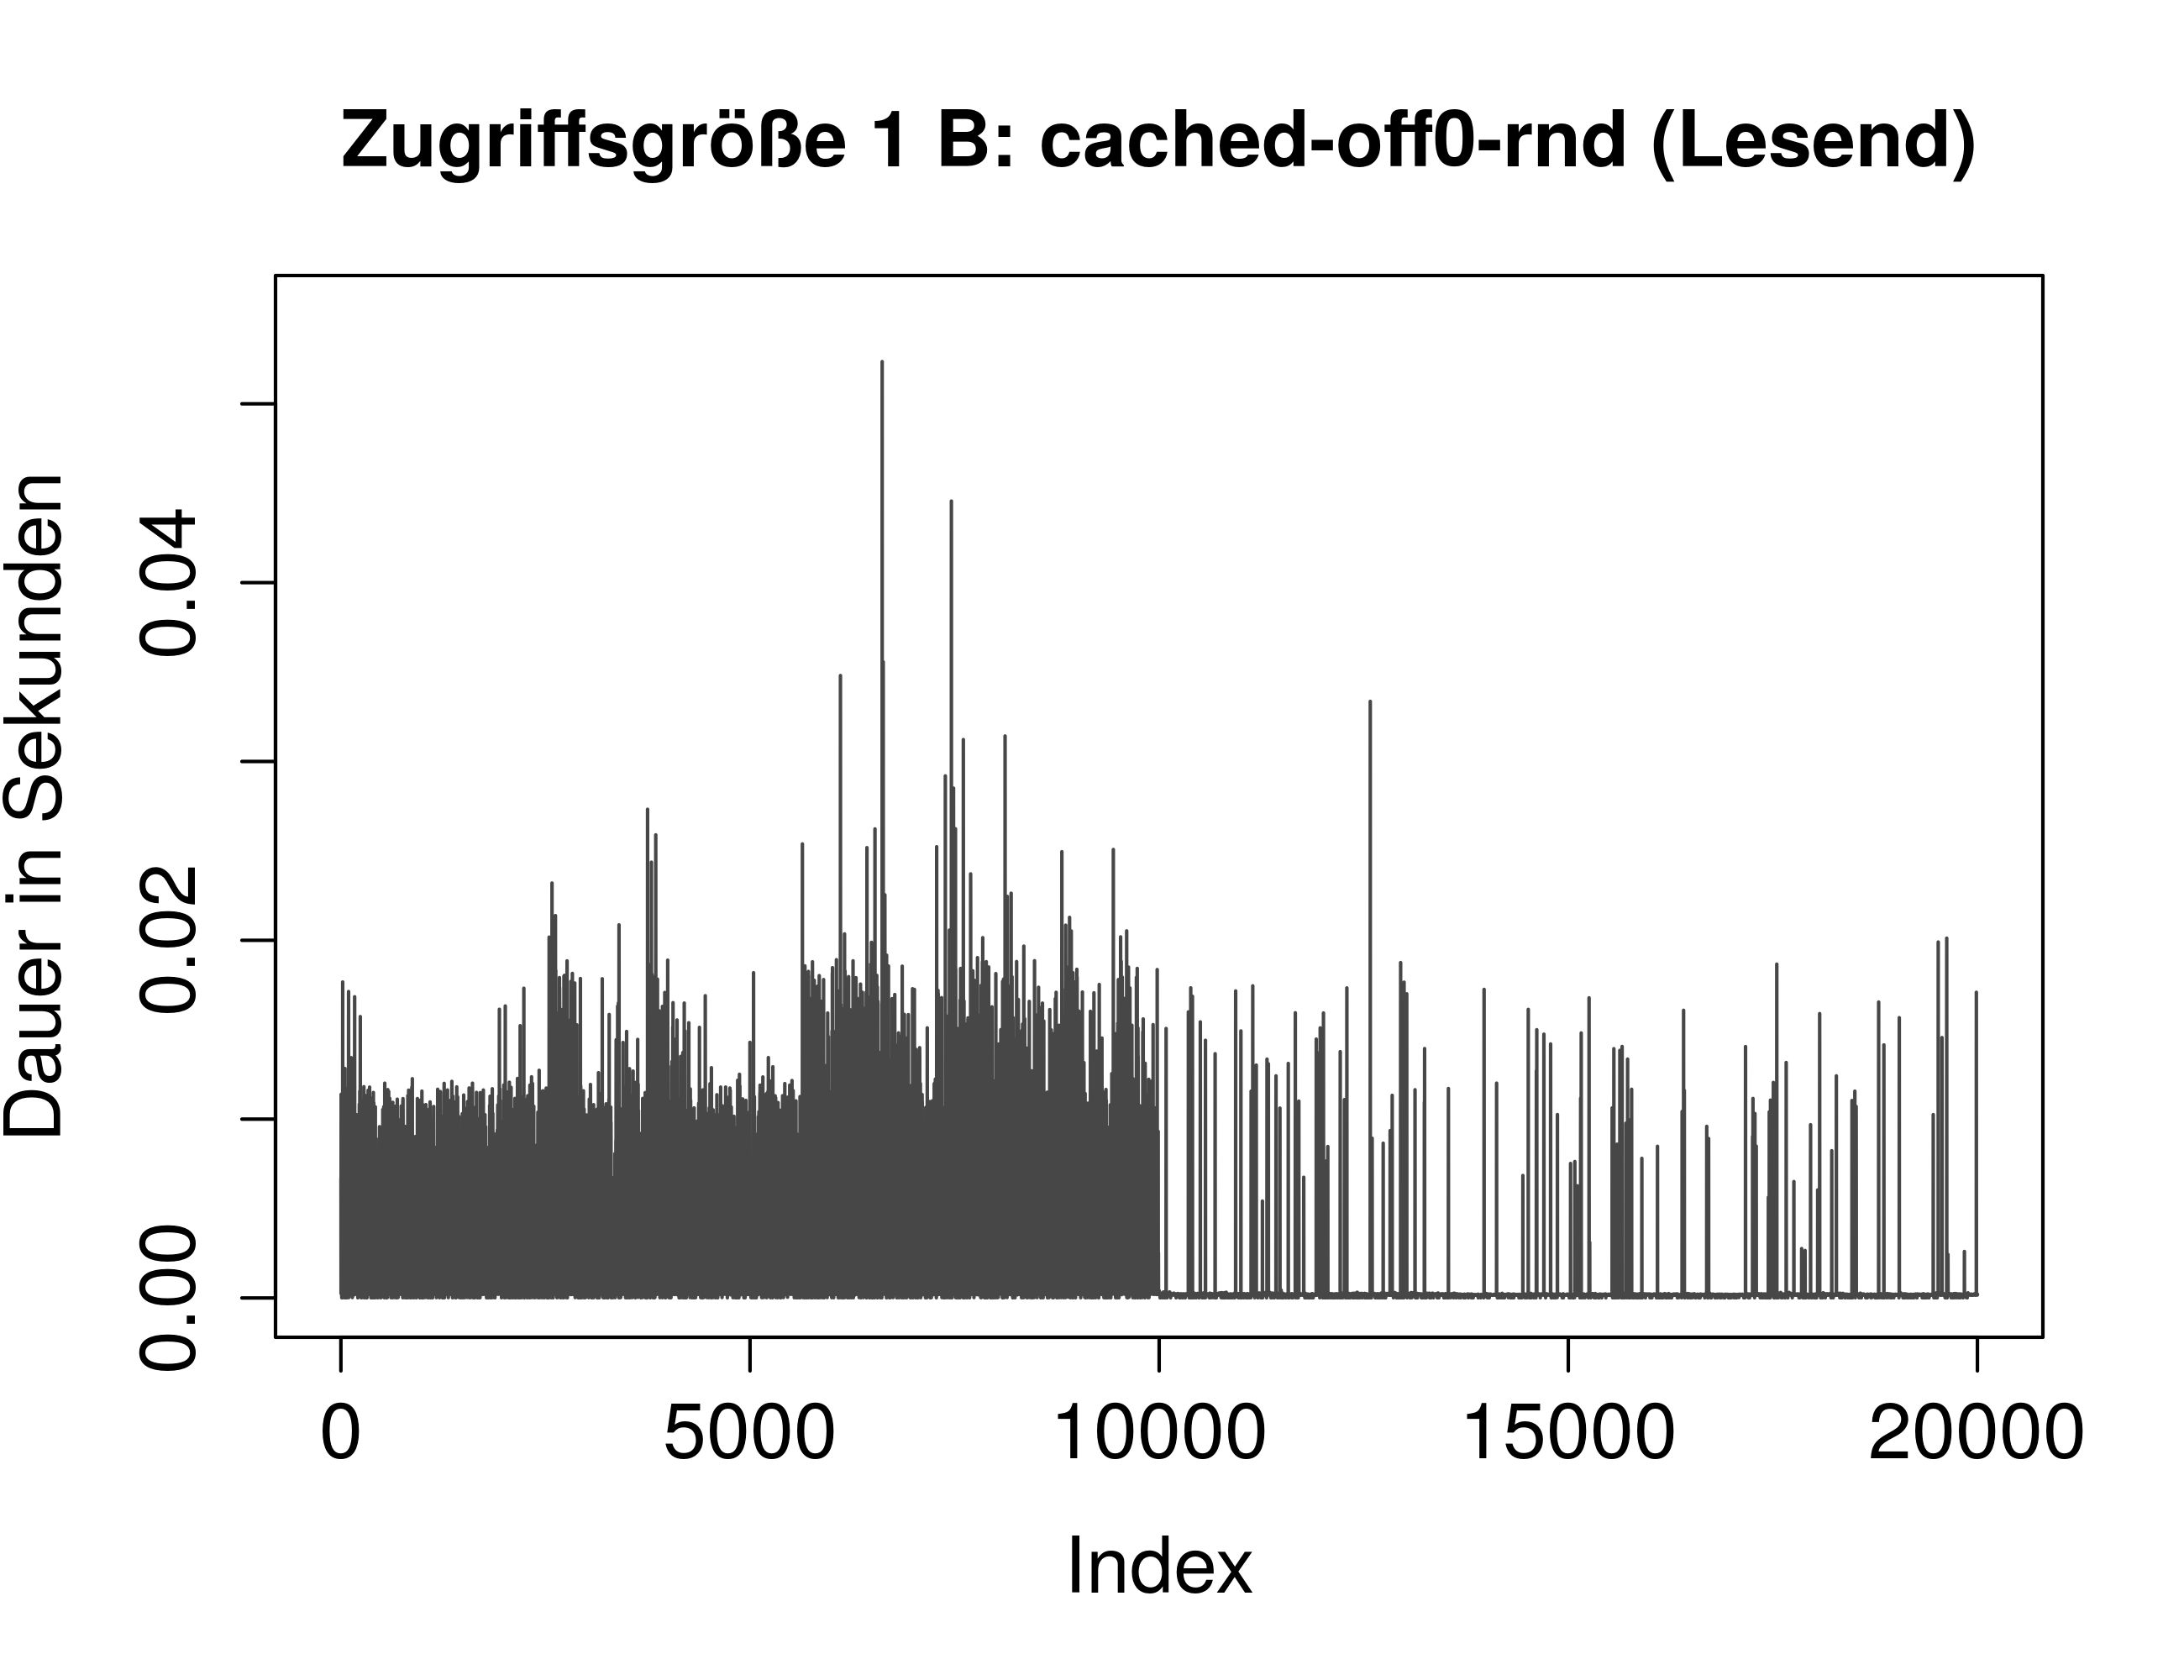
\includegraphics[width=.43\textwidth]{Bilder/Plots/exploration/plot_Size1_read_rnd.png}
	}
	\hfill
	\subfloat{
		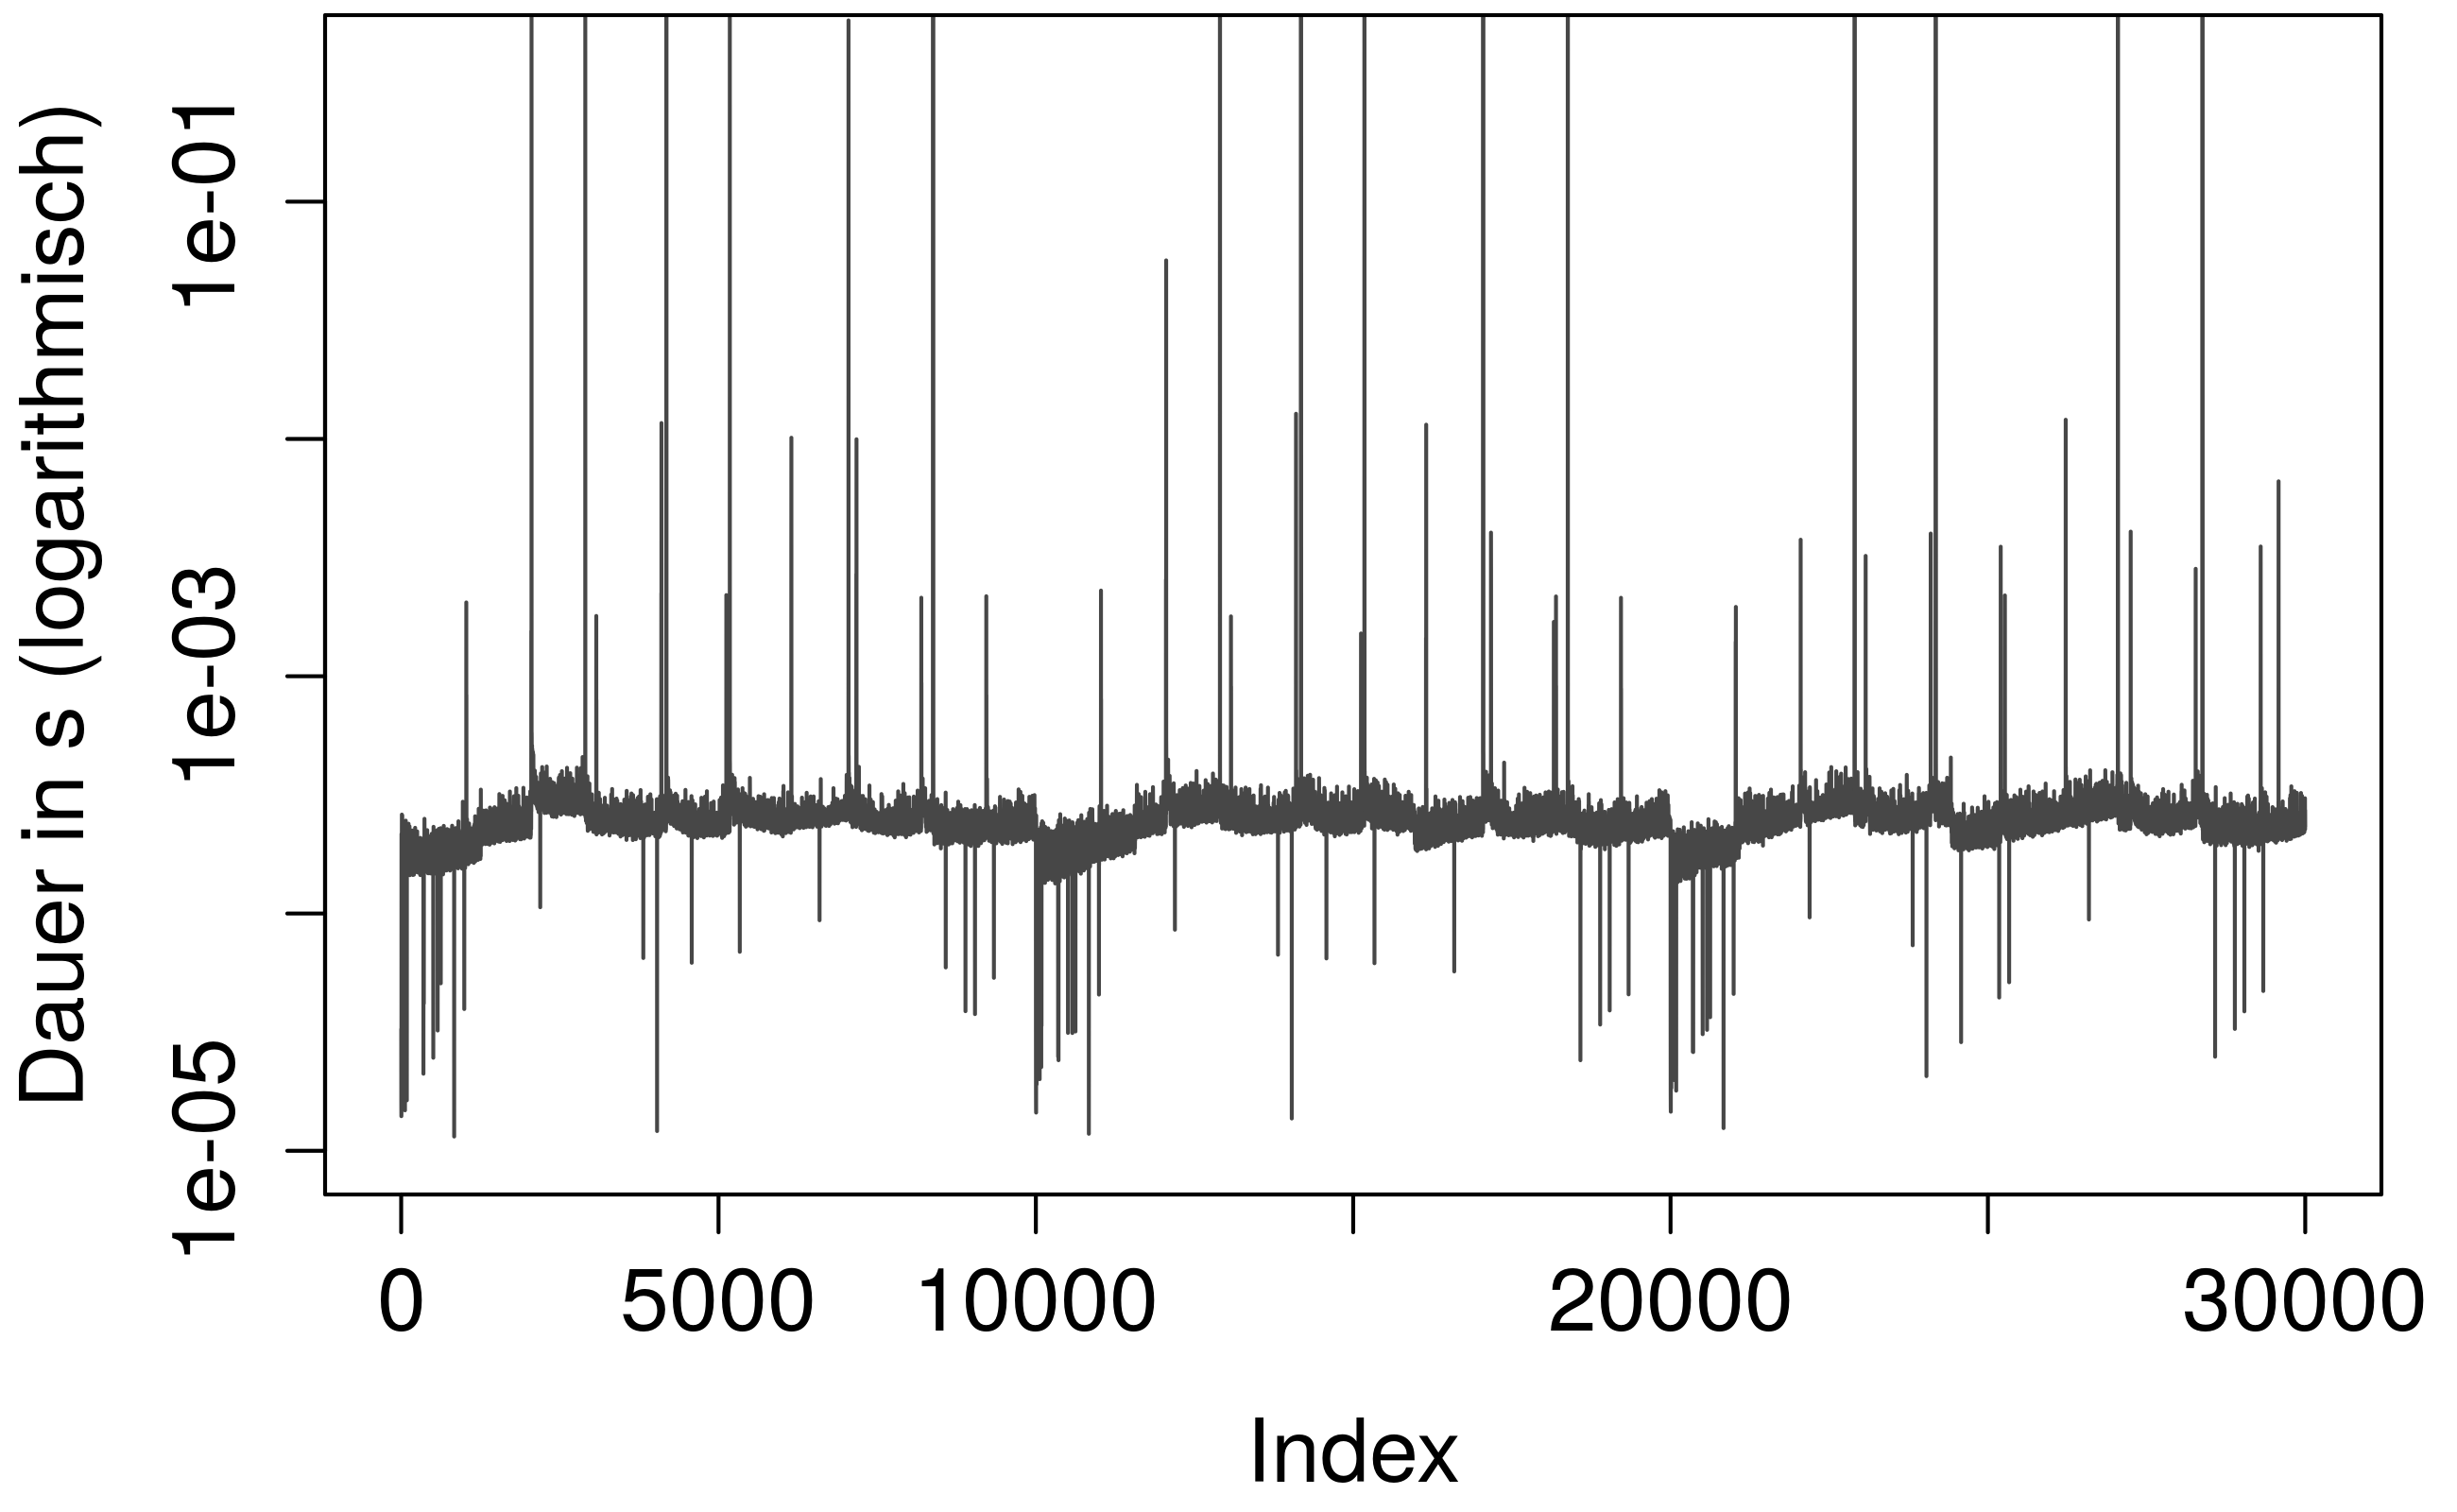
\includegraphics[width=.43\textwidth]{Bilder/Plots/exploration/plot_Size1_write_rnd.png}
	}		
	\caption{Detailbetrachtung aller Messungen mit Zugriffsgröße 1KB}
	\label{fig:groesse1}
\end{figure} 

\begin{figure}
	\subfloat{
		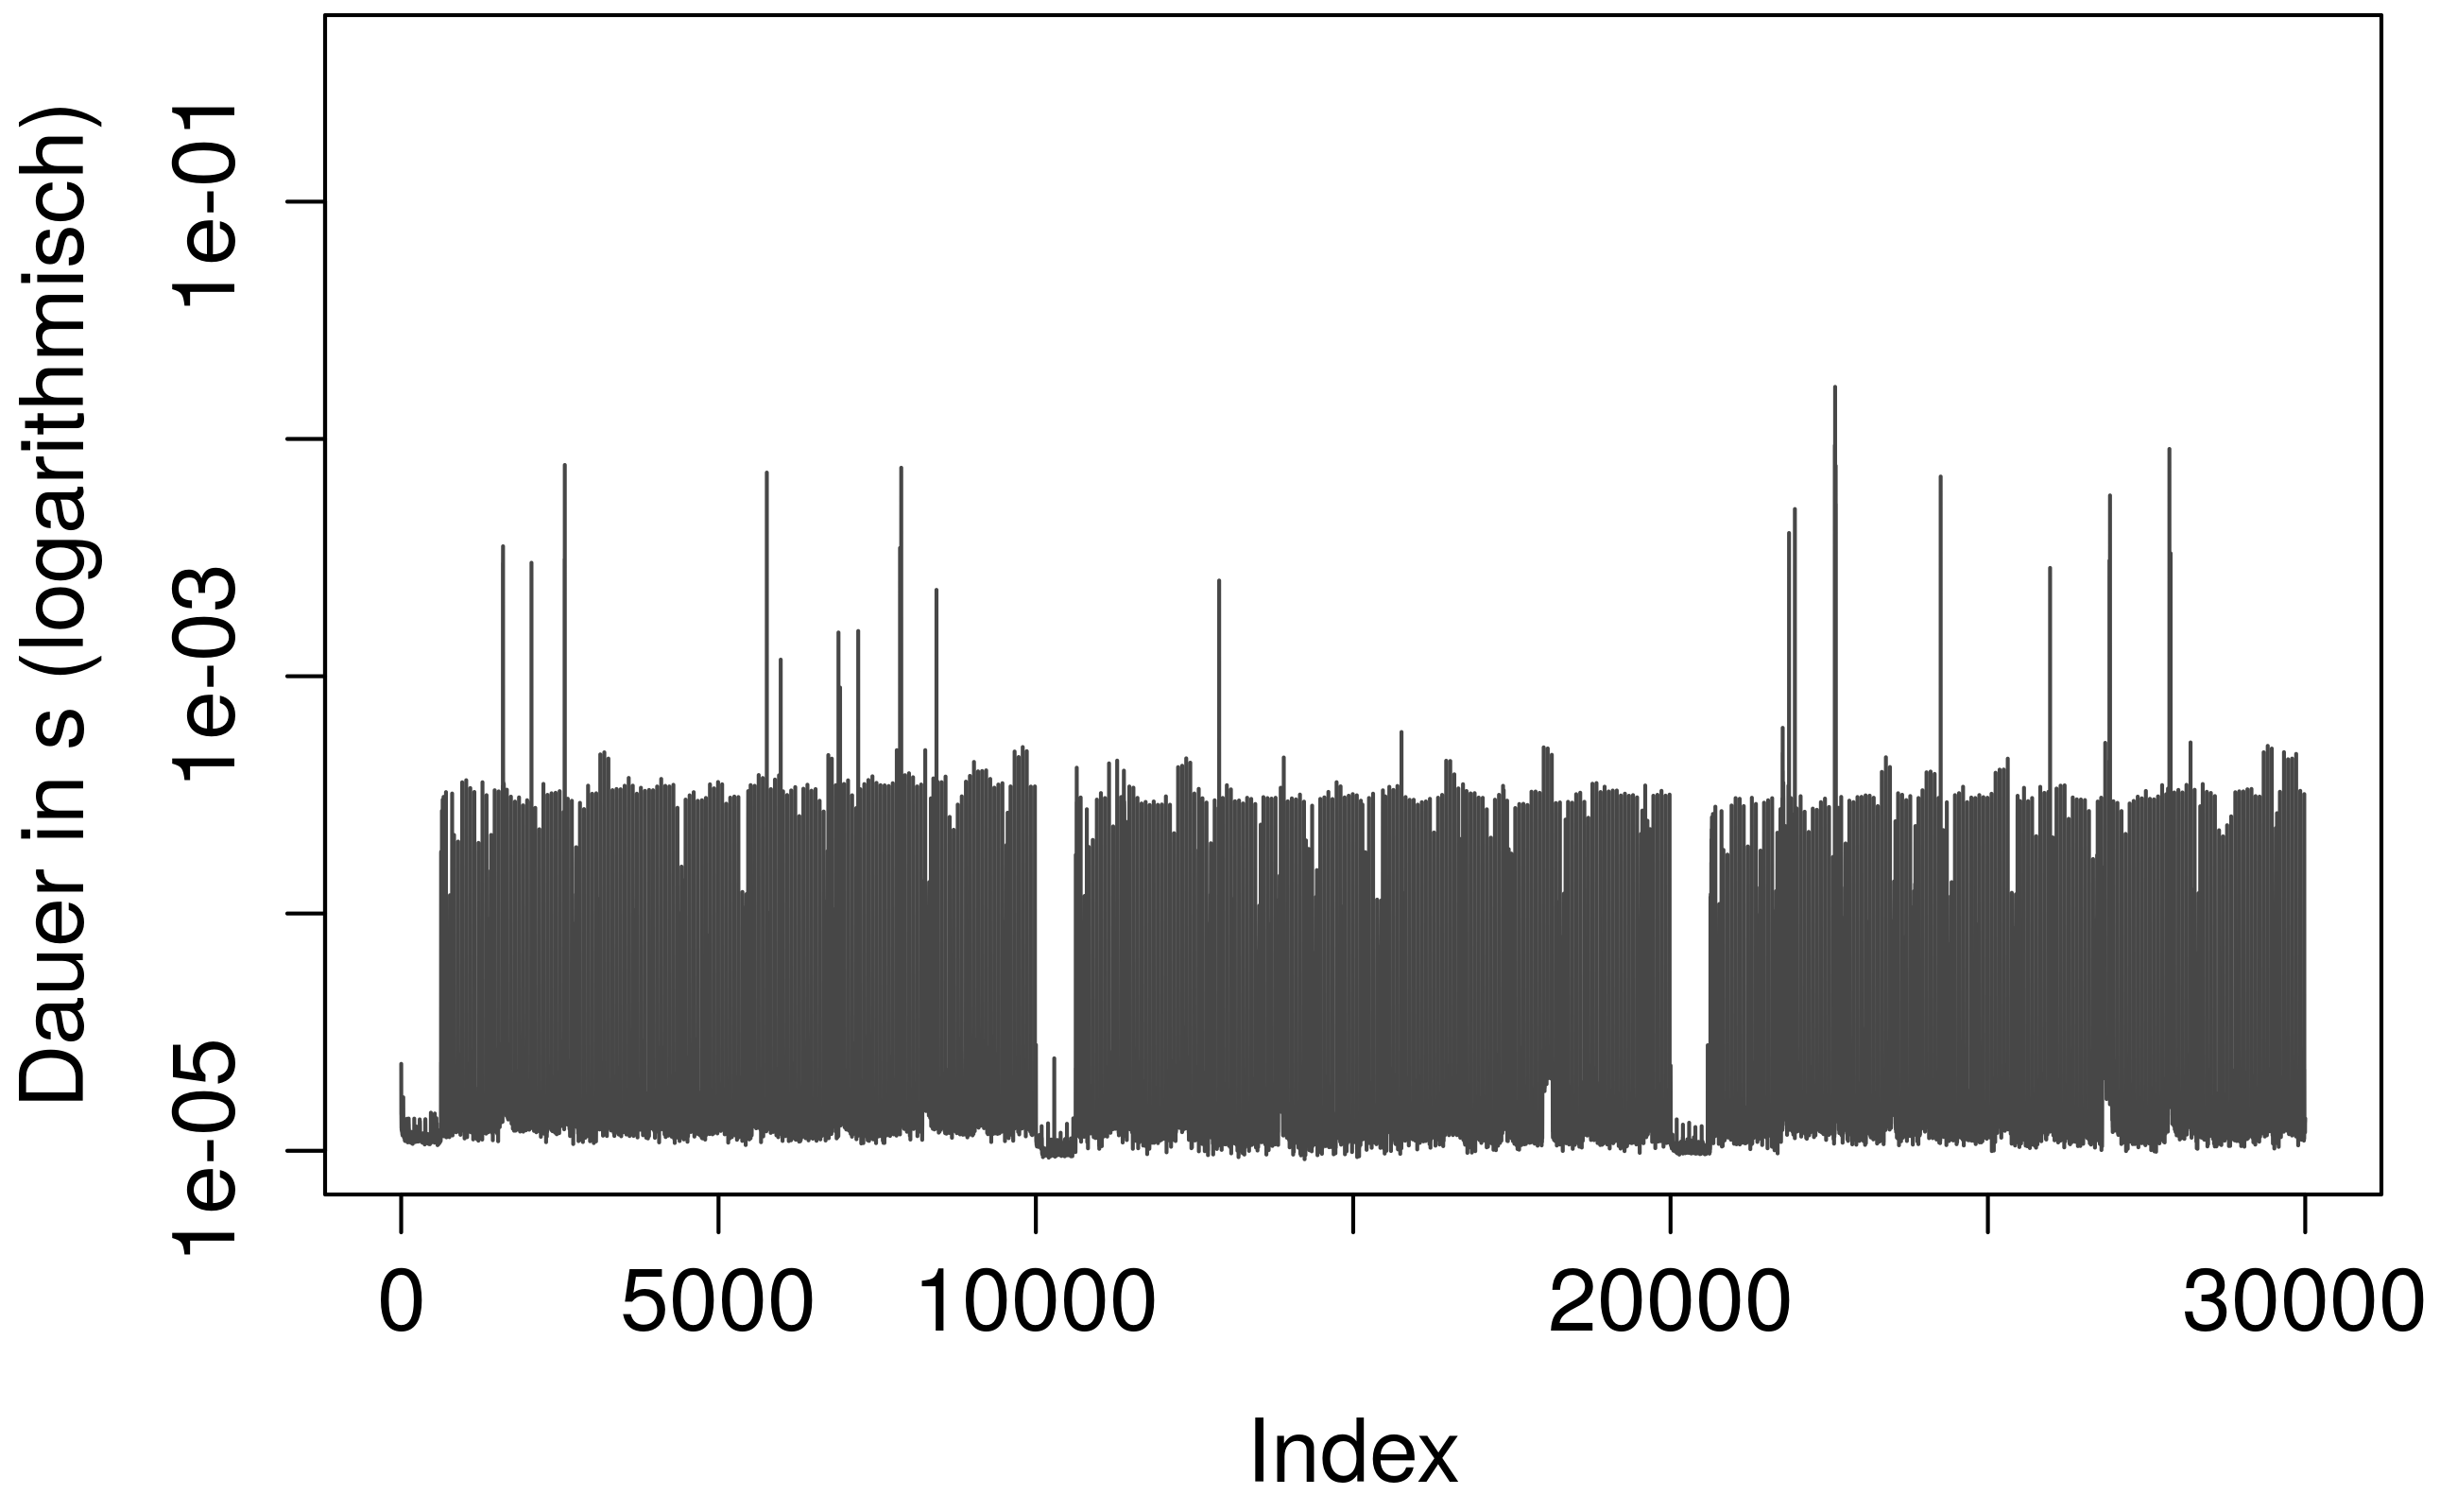
\includegraphics[width=.43\textwidth]{Bilder/Plots/exploration/plot_Size16384_read_seq.png}
	}
	\hfill
	\subfloat{
		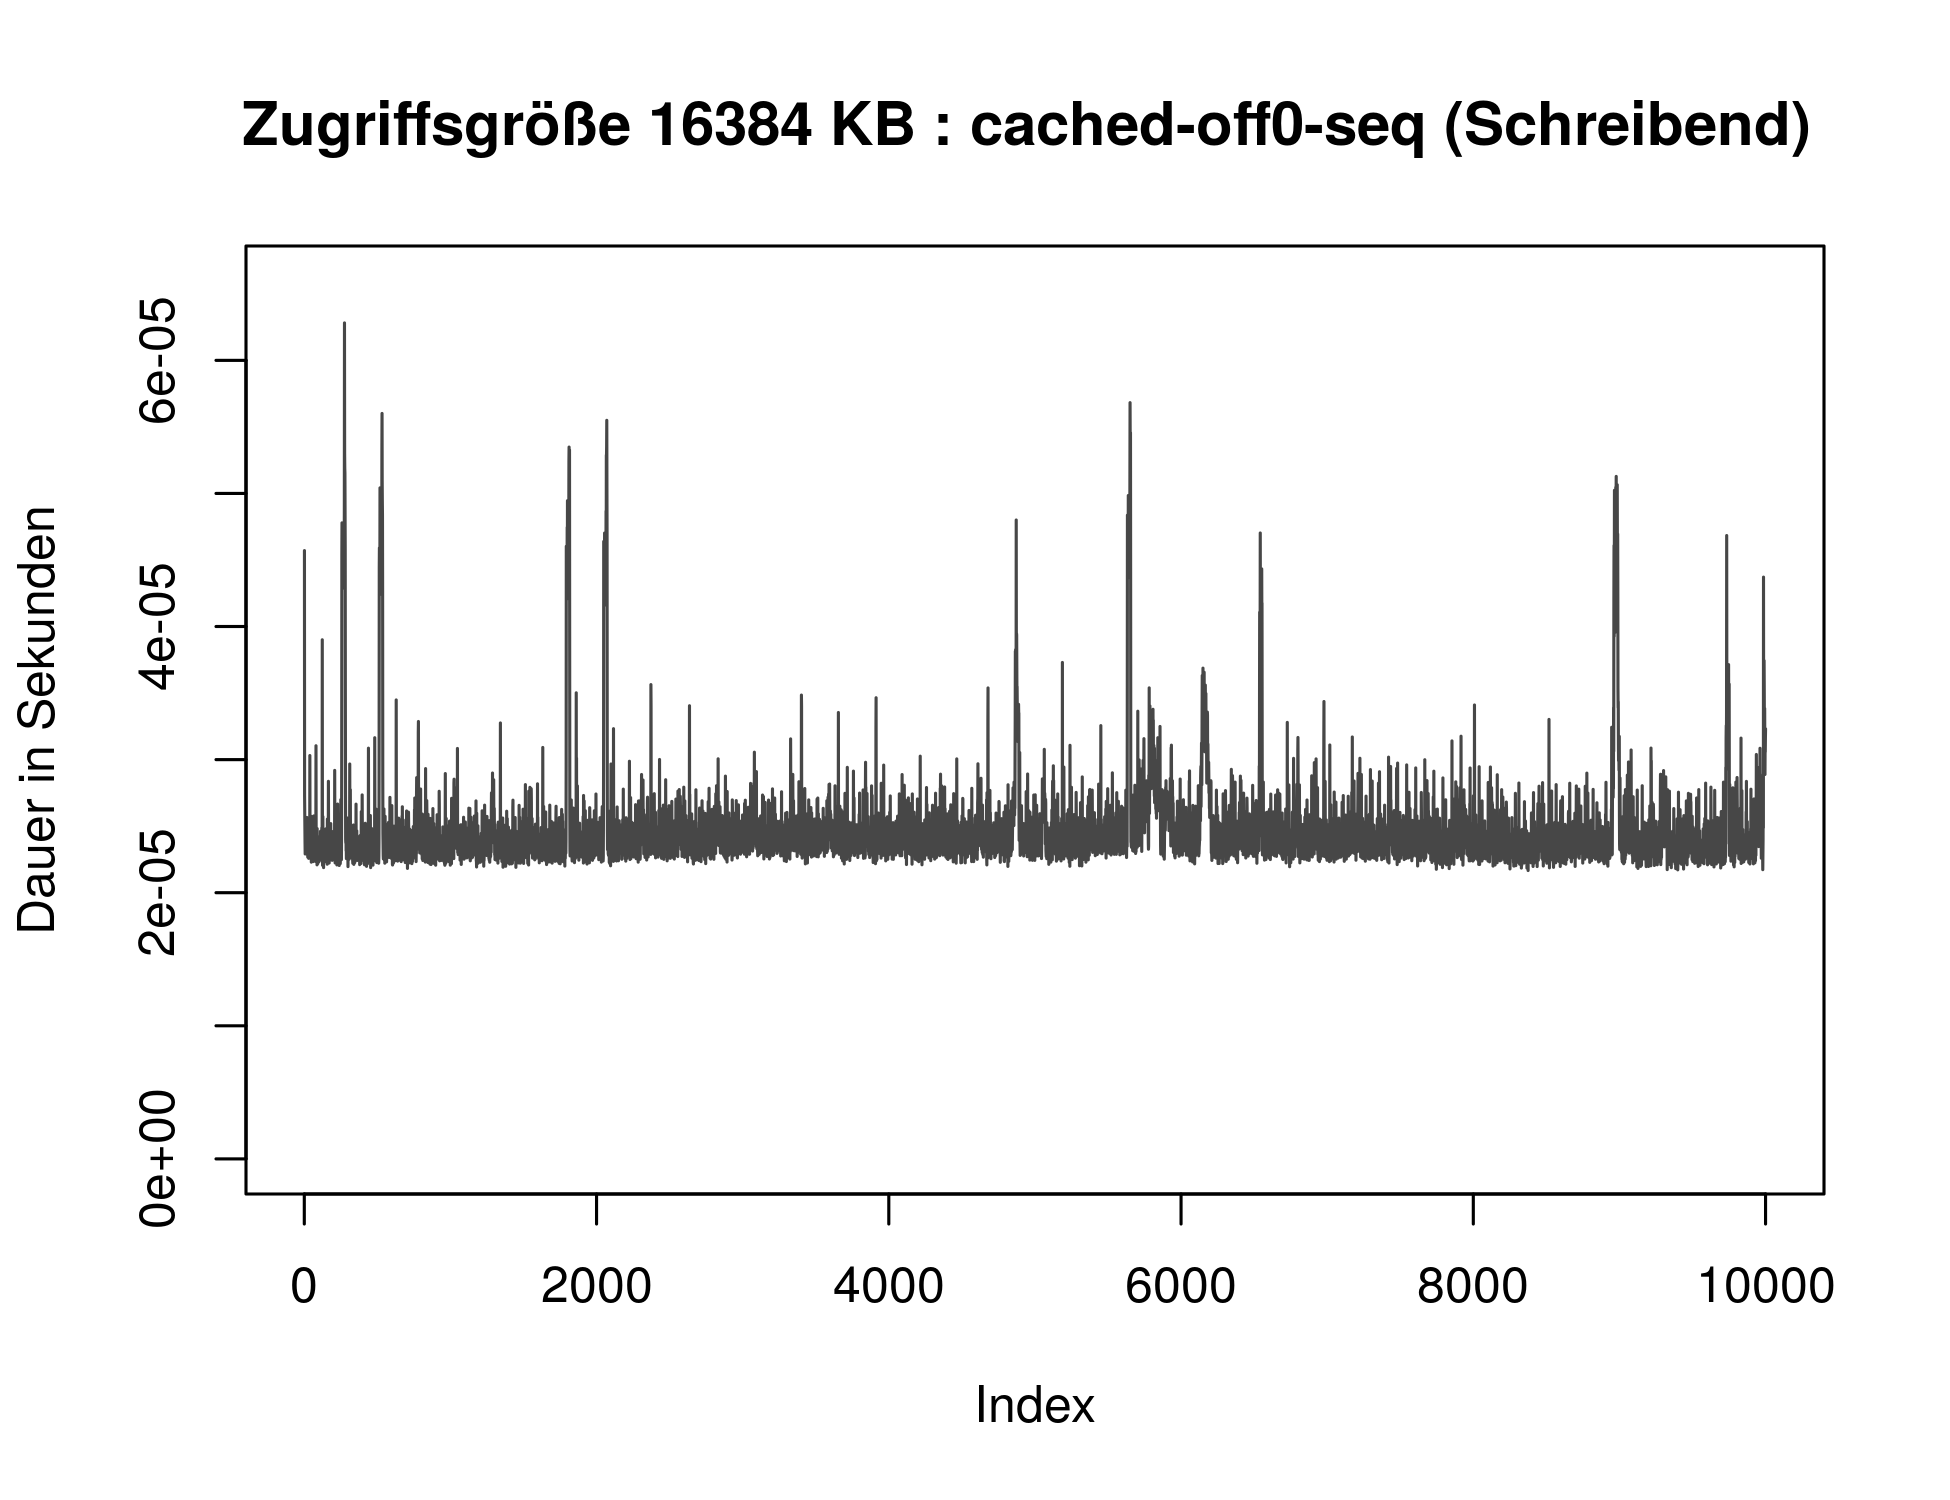
\includegraphics[width=.43\textwidth]{Bilder/Plots/exploration/plot_Size16384_write_seq.png}
	}\\
	\subfloat{
		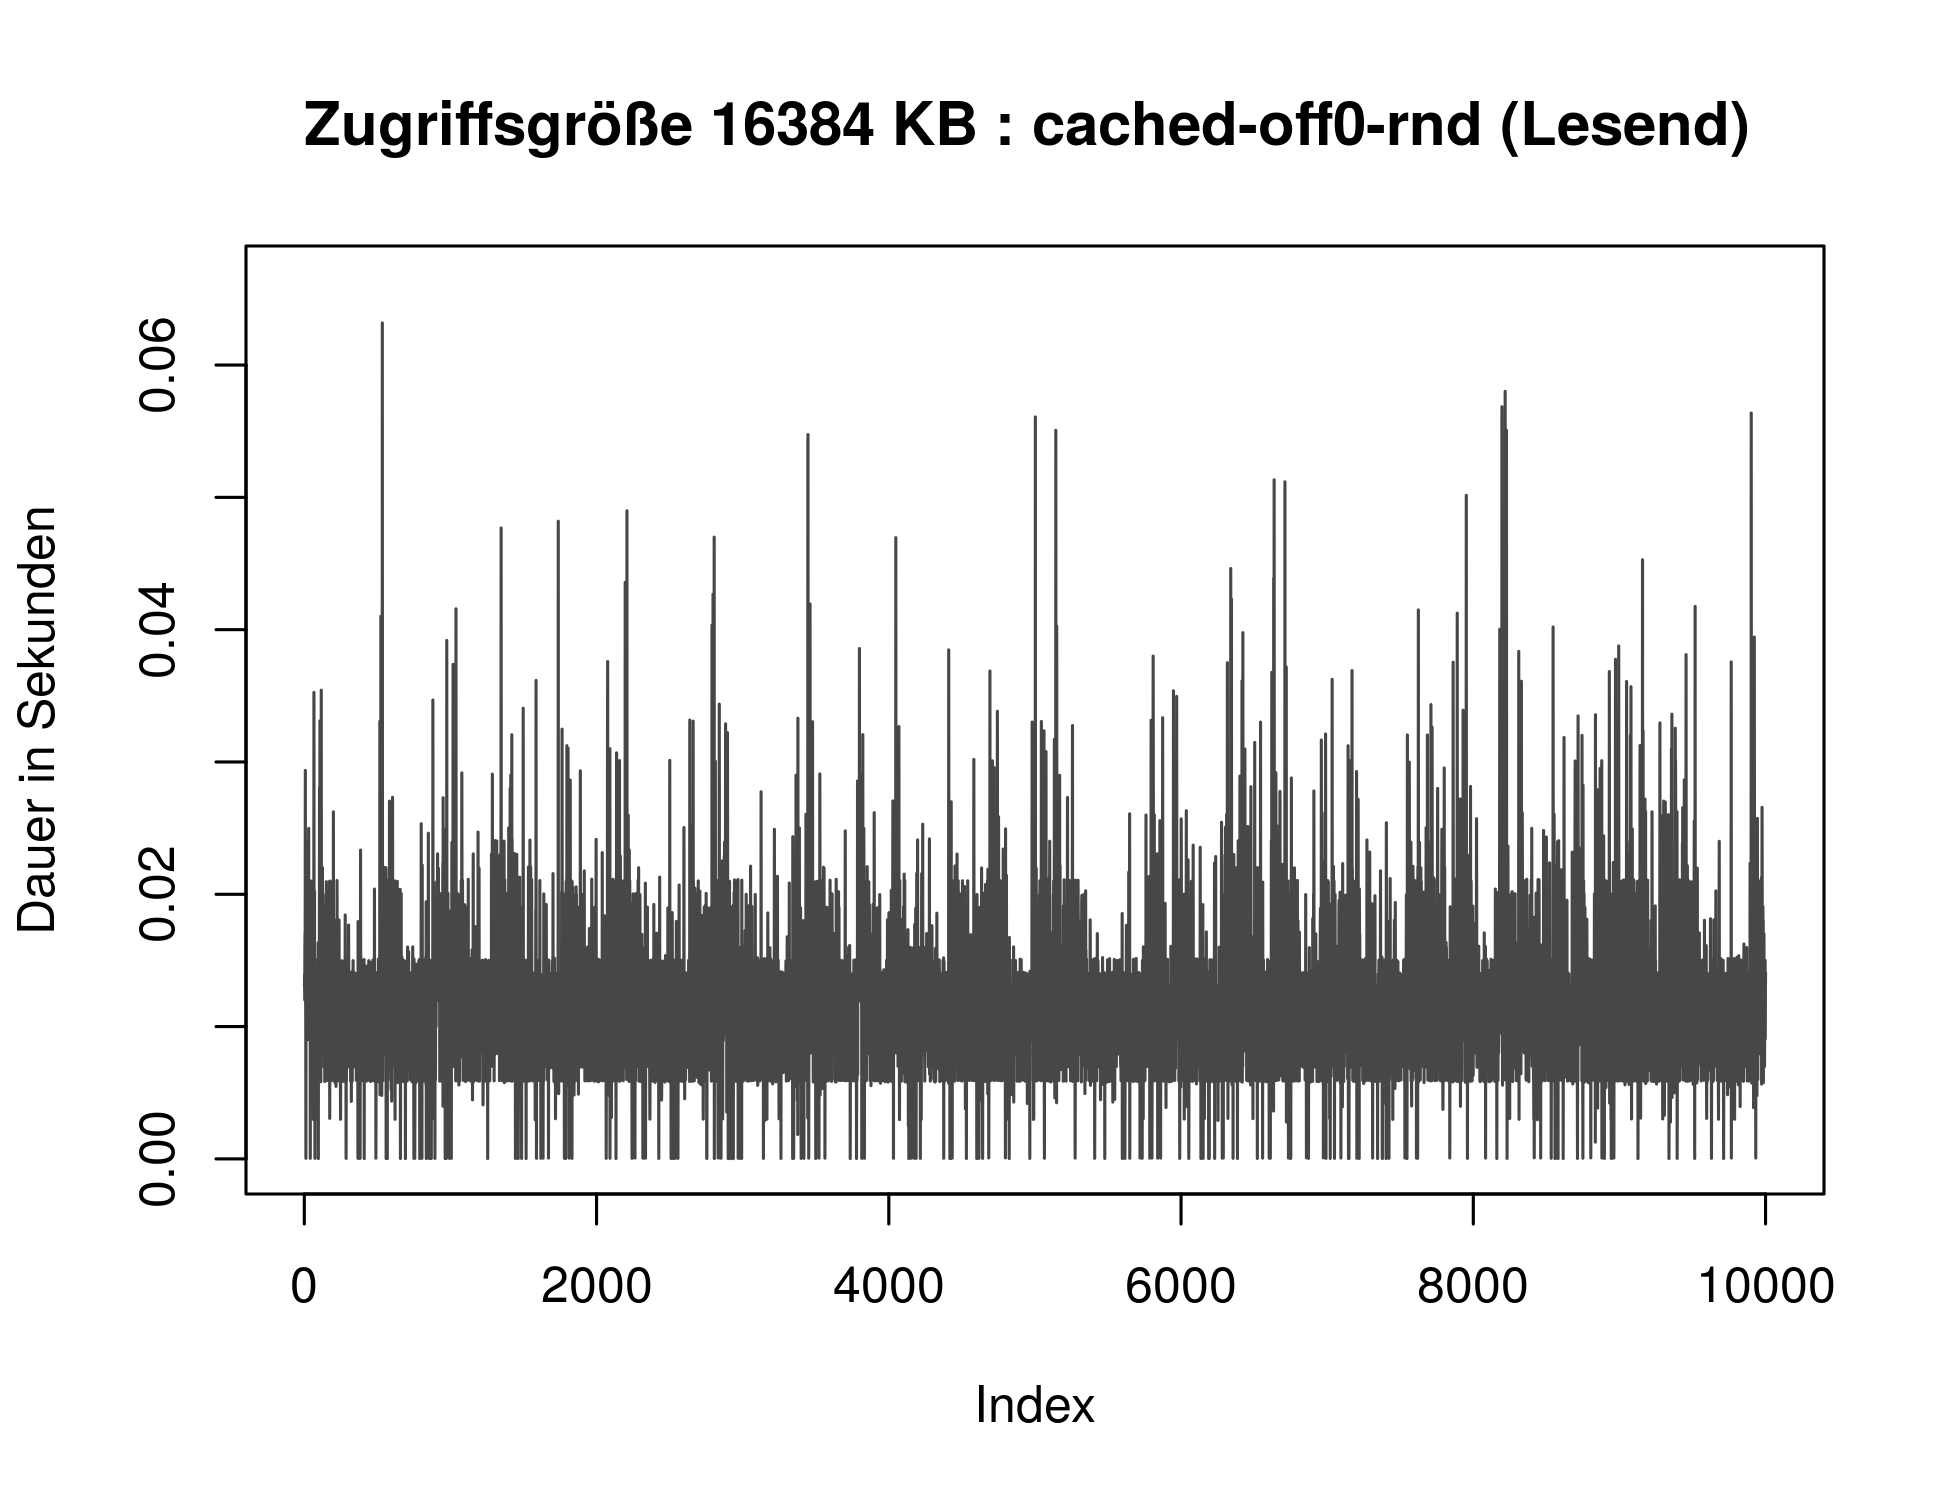
\includegraphics[width=.43\textwidth]{Bilder/Plots/exploration/plot_Size16384_read_rnd.png}
	}
	\hfill
	\subfloat{
		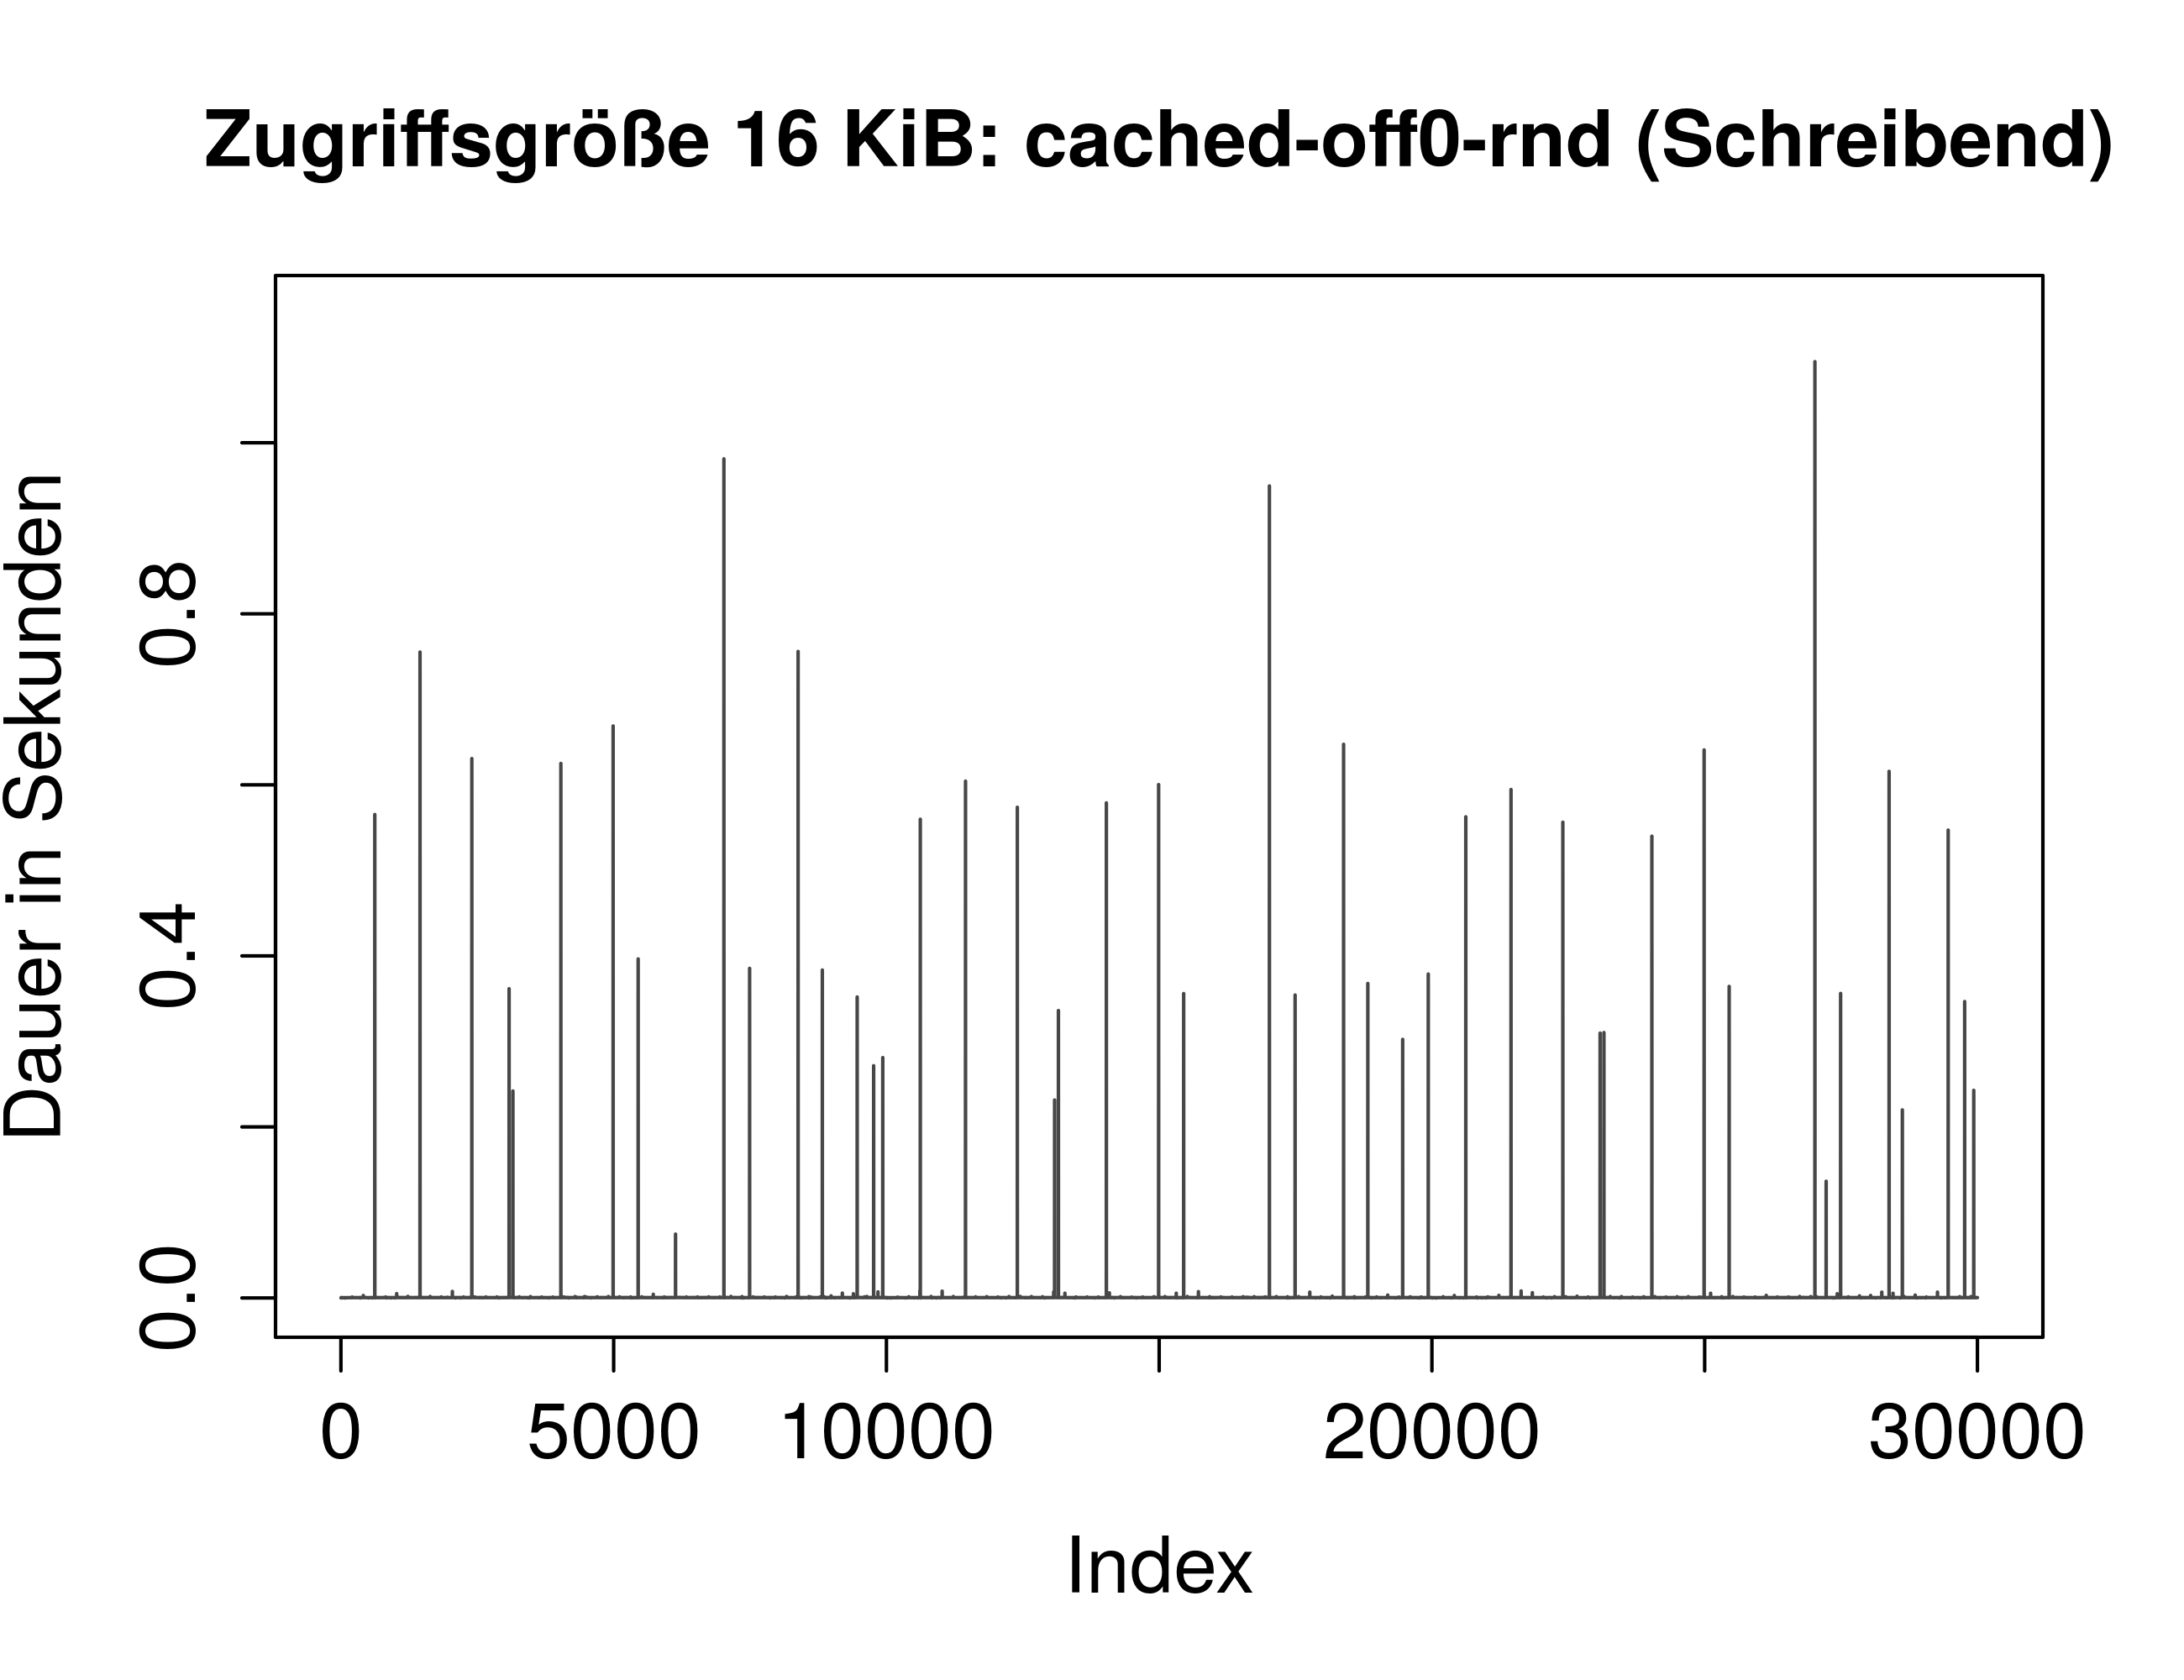
\includegraphics[width=.43\textwidth]{Bilder/Plots/exploration/plot_Size16384_write_rnd.png}
	}		
	\caption{Detailbetrachtung aller Messungen mit Zugriffsgröße 16384KB}
	\label{fig:groesse16384}
\end{figure} 

\begin{figure}
	\subfloat{
		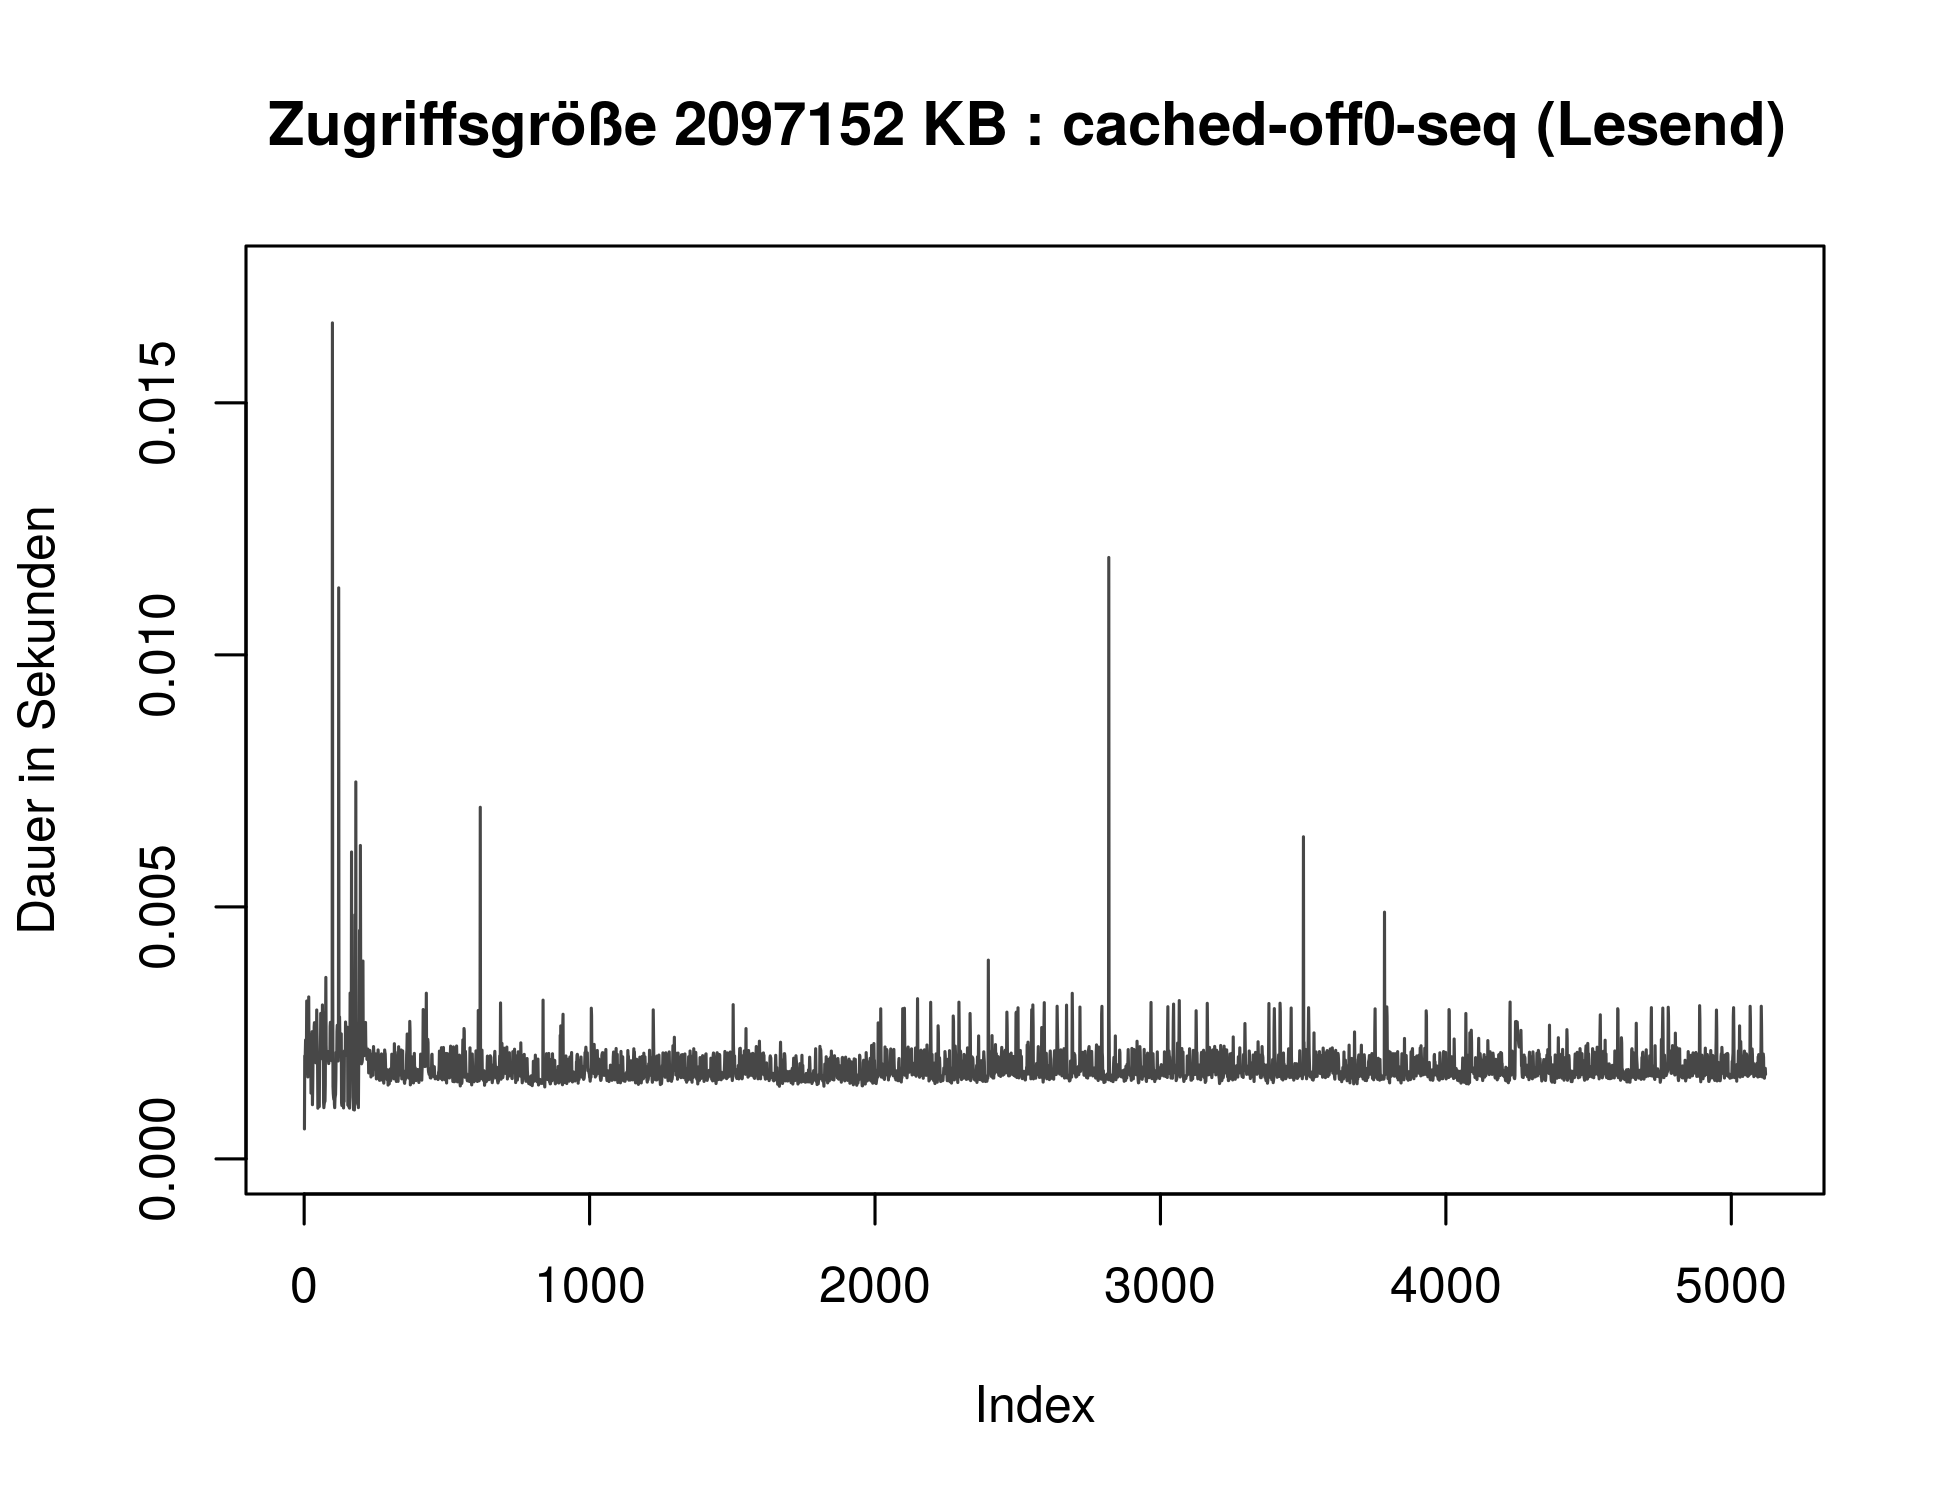
\includegraphics[width=.43\textwidth]{Bilder/Plots/exploration/plot_Size2097152_read_seq.png}
	}
	\hfill
	\subfloat{
		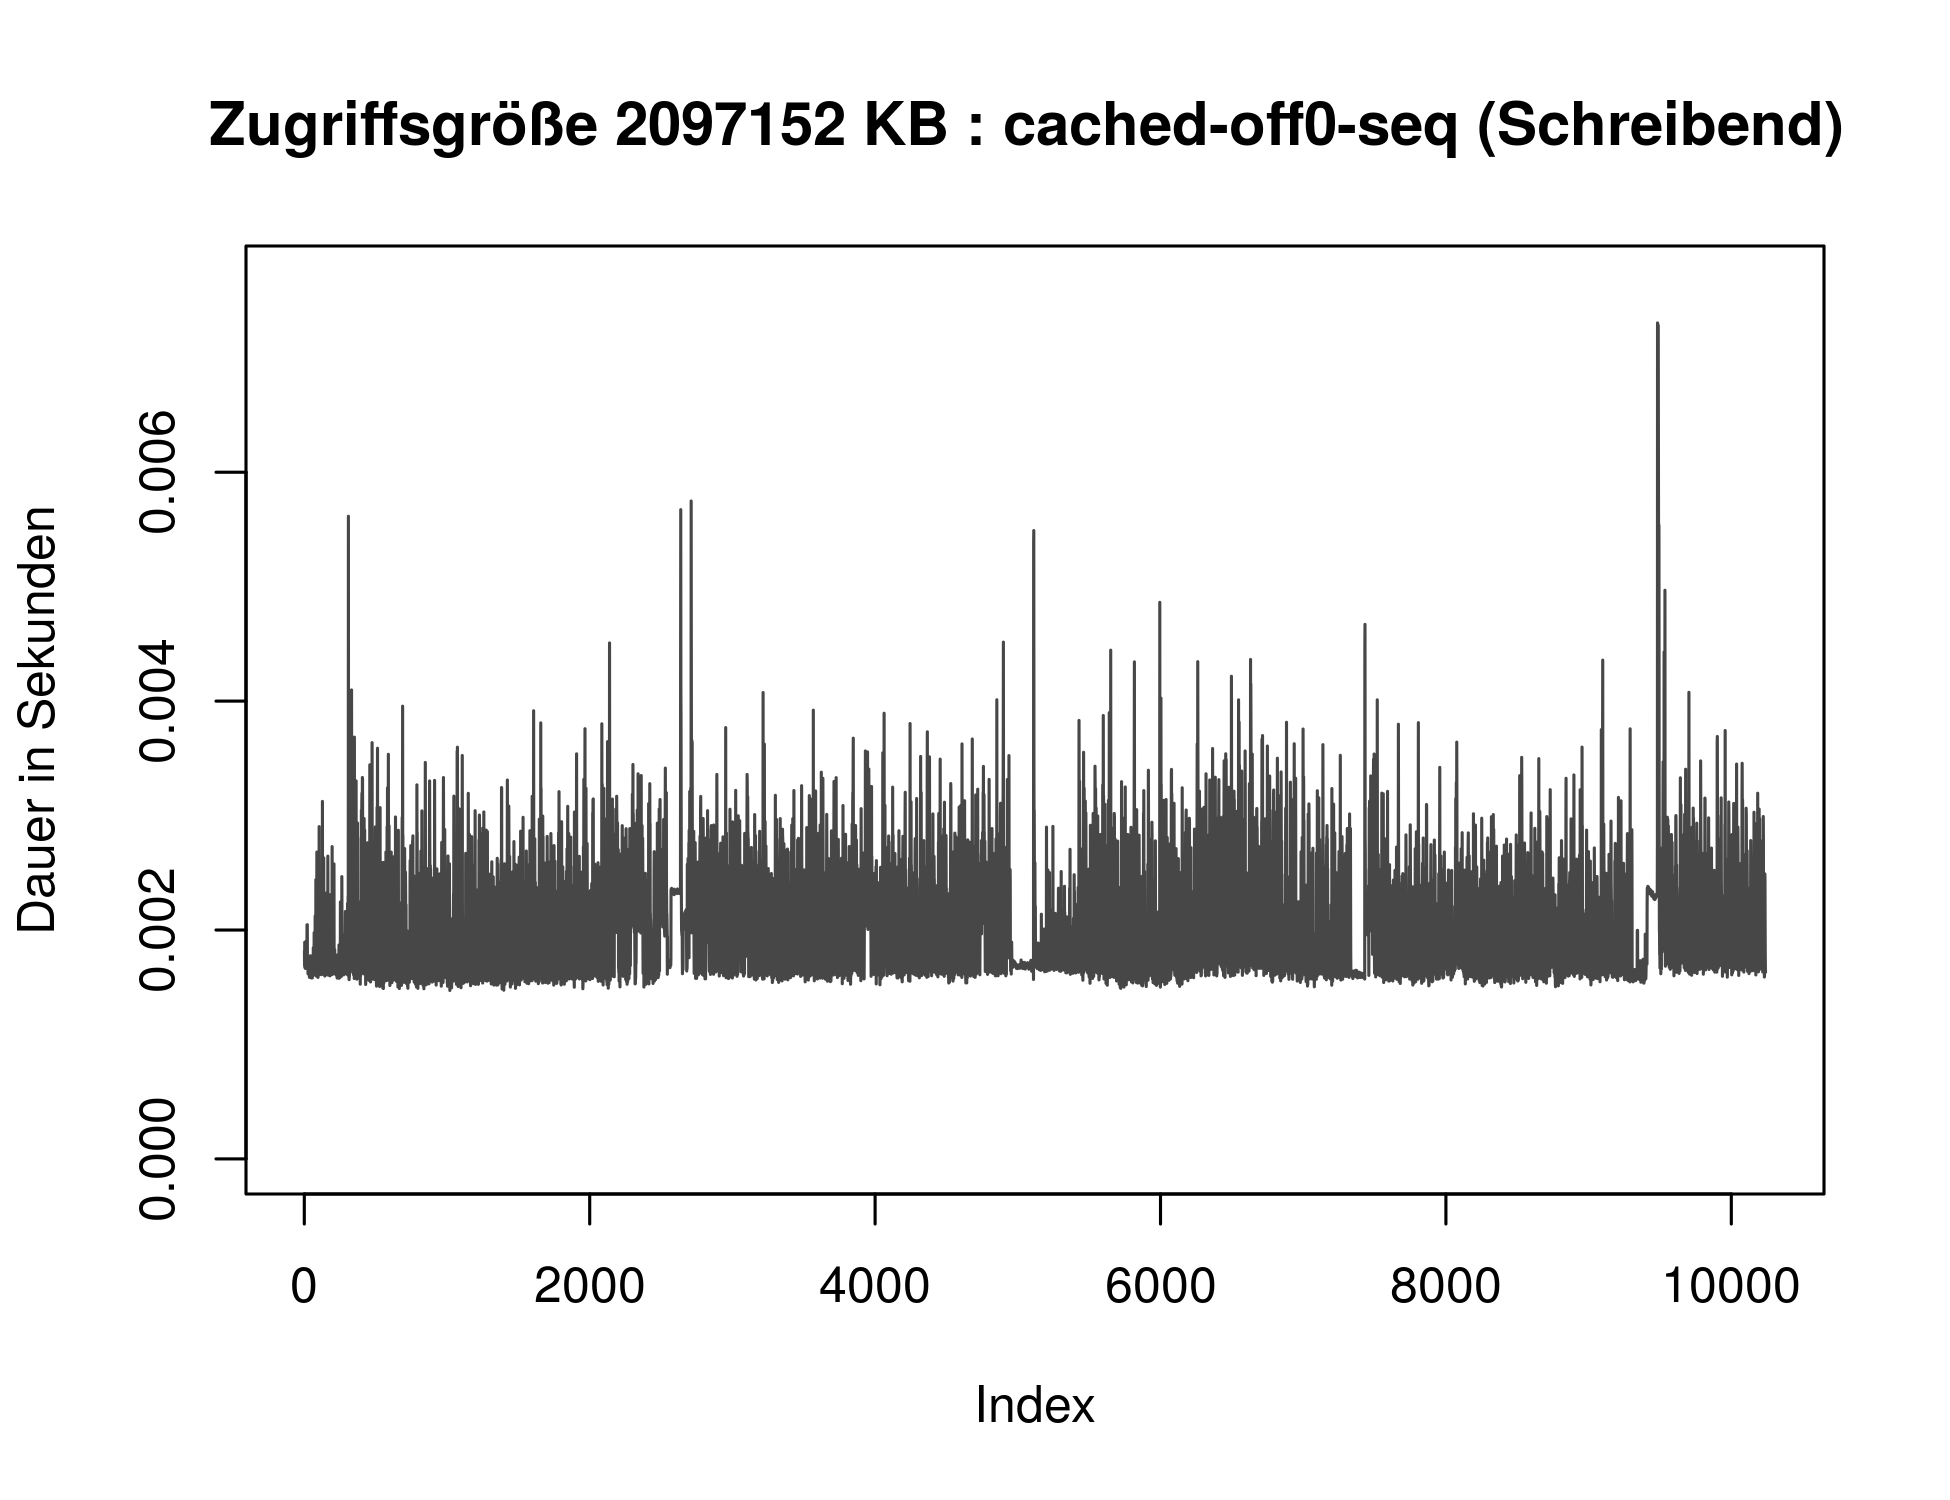
\includegraphics[width=.43\textwidth]{Bilder/Plots/exploration/plot_Size2097152_write_seq.png}
	}\\
	\subfloat{
		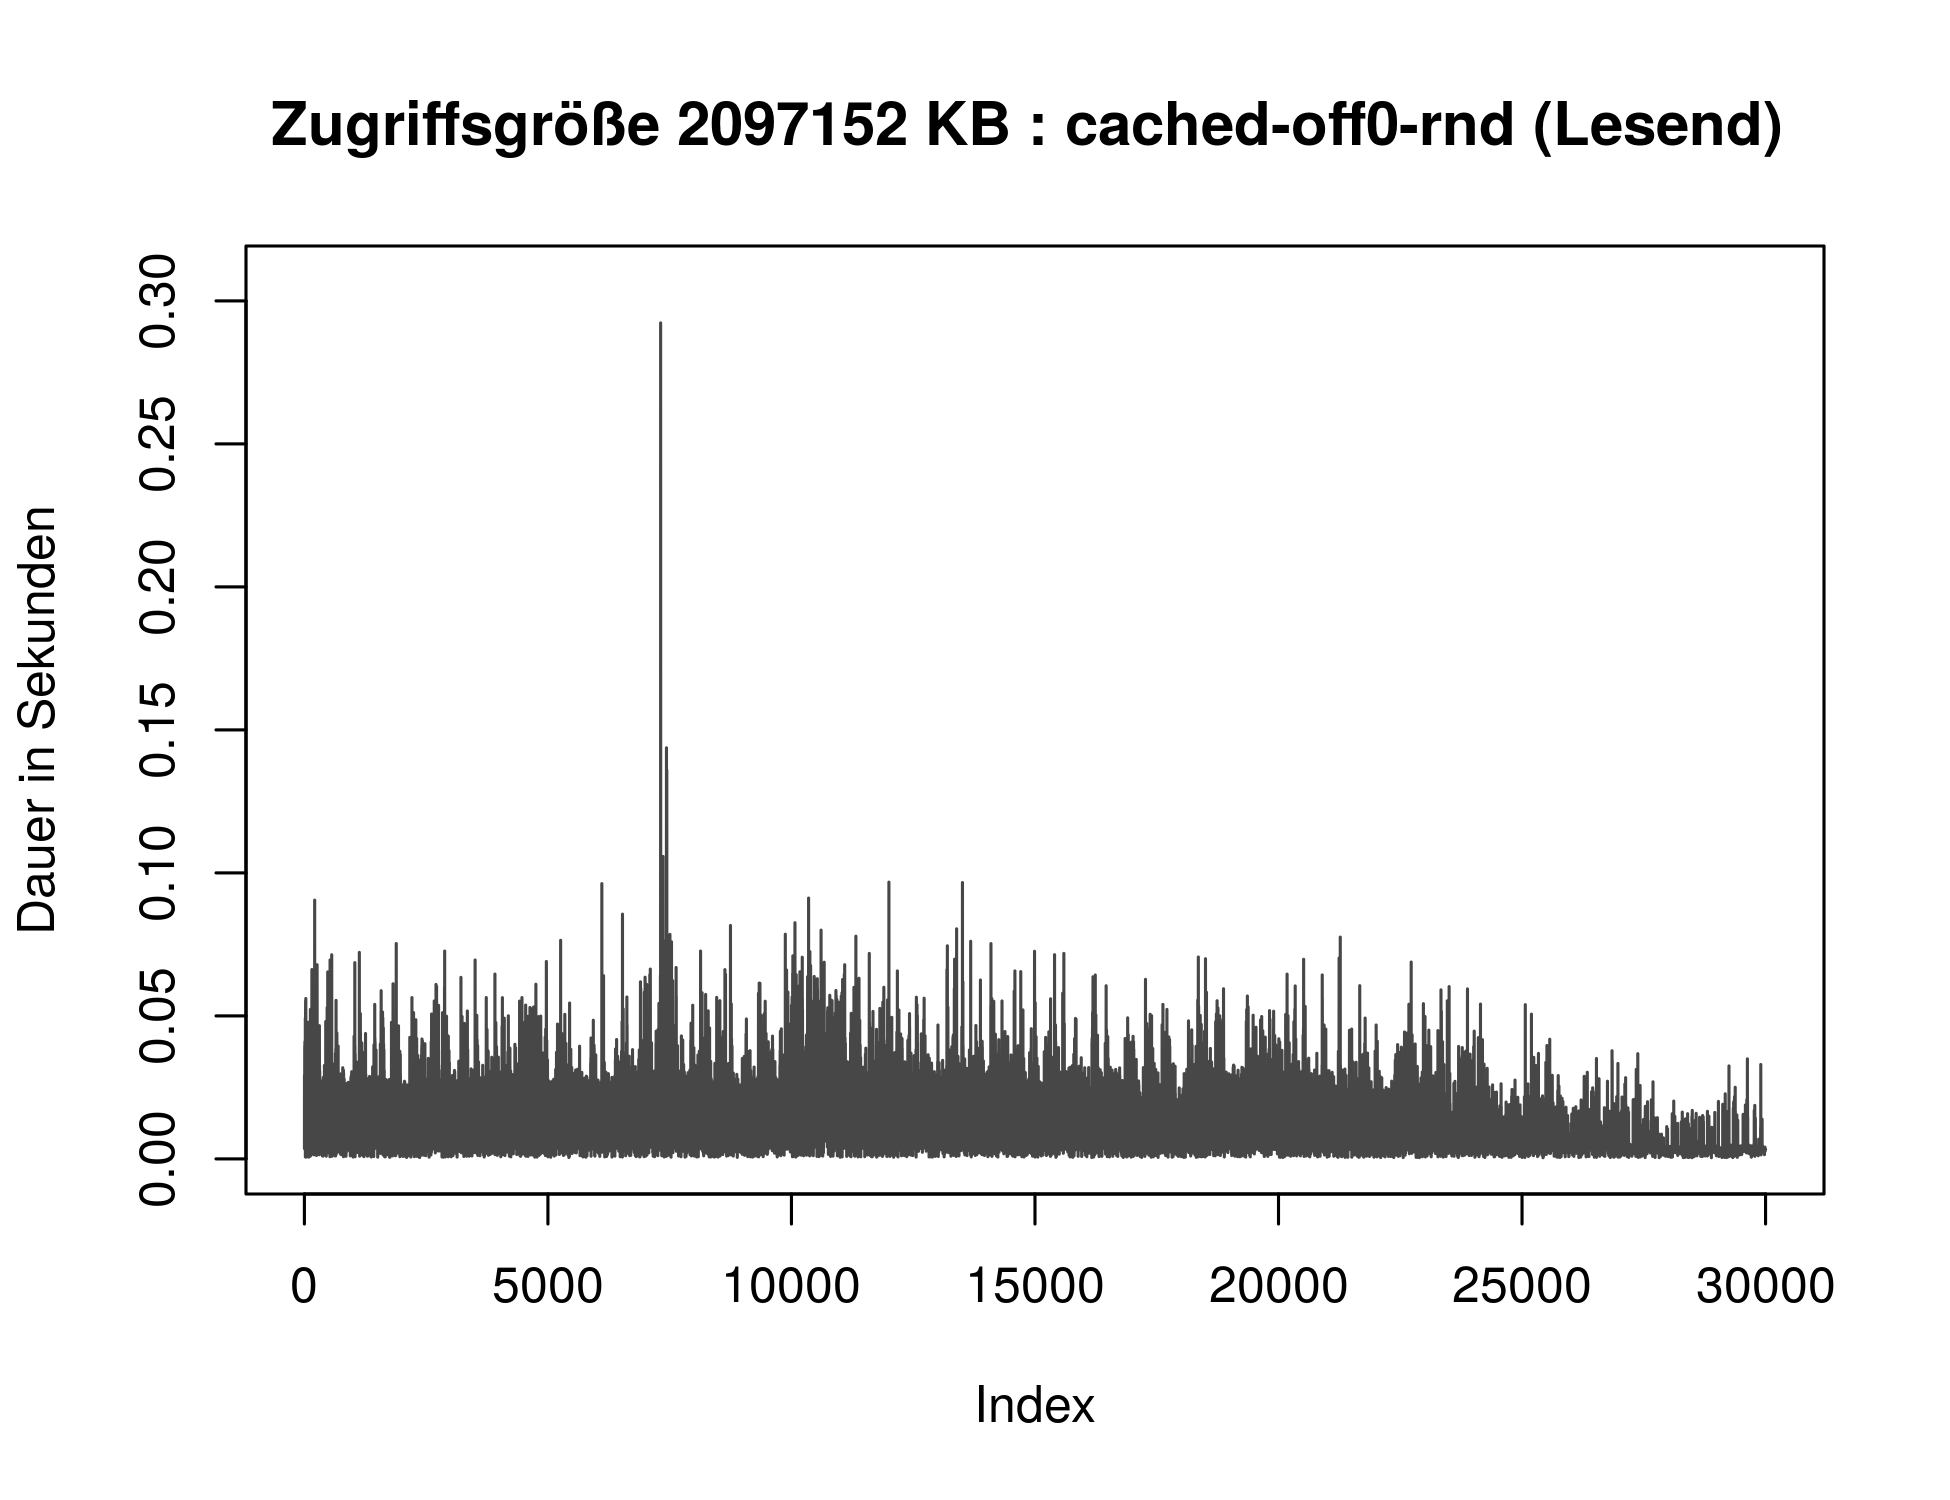
\includegraphics[width=.43\textwidth]{Bilder/Plots/exploration/plot_Size2097152_read_rnd.png}
	}
	\hfill
	\subfloat{
		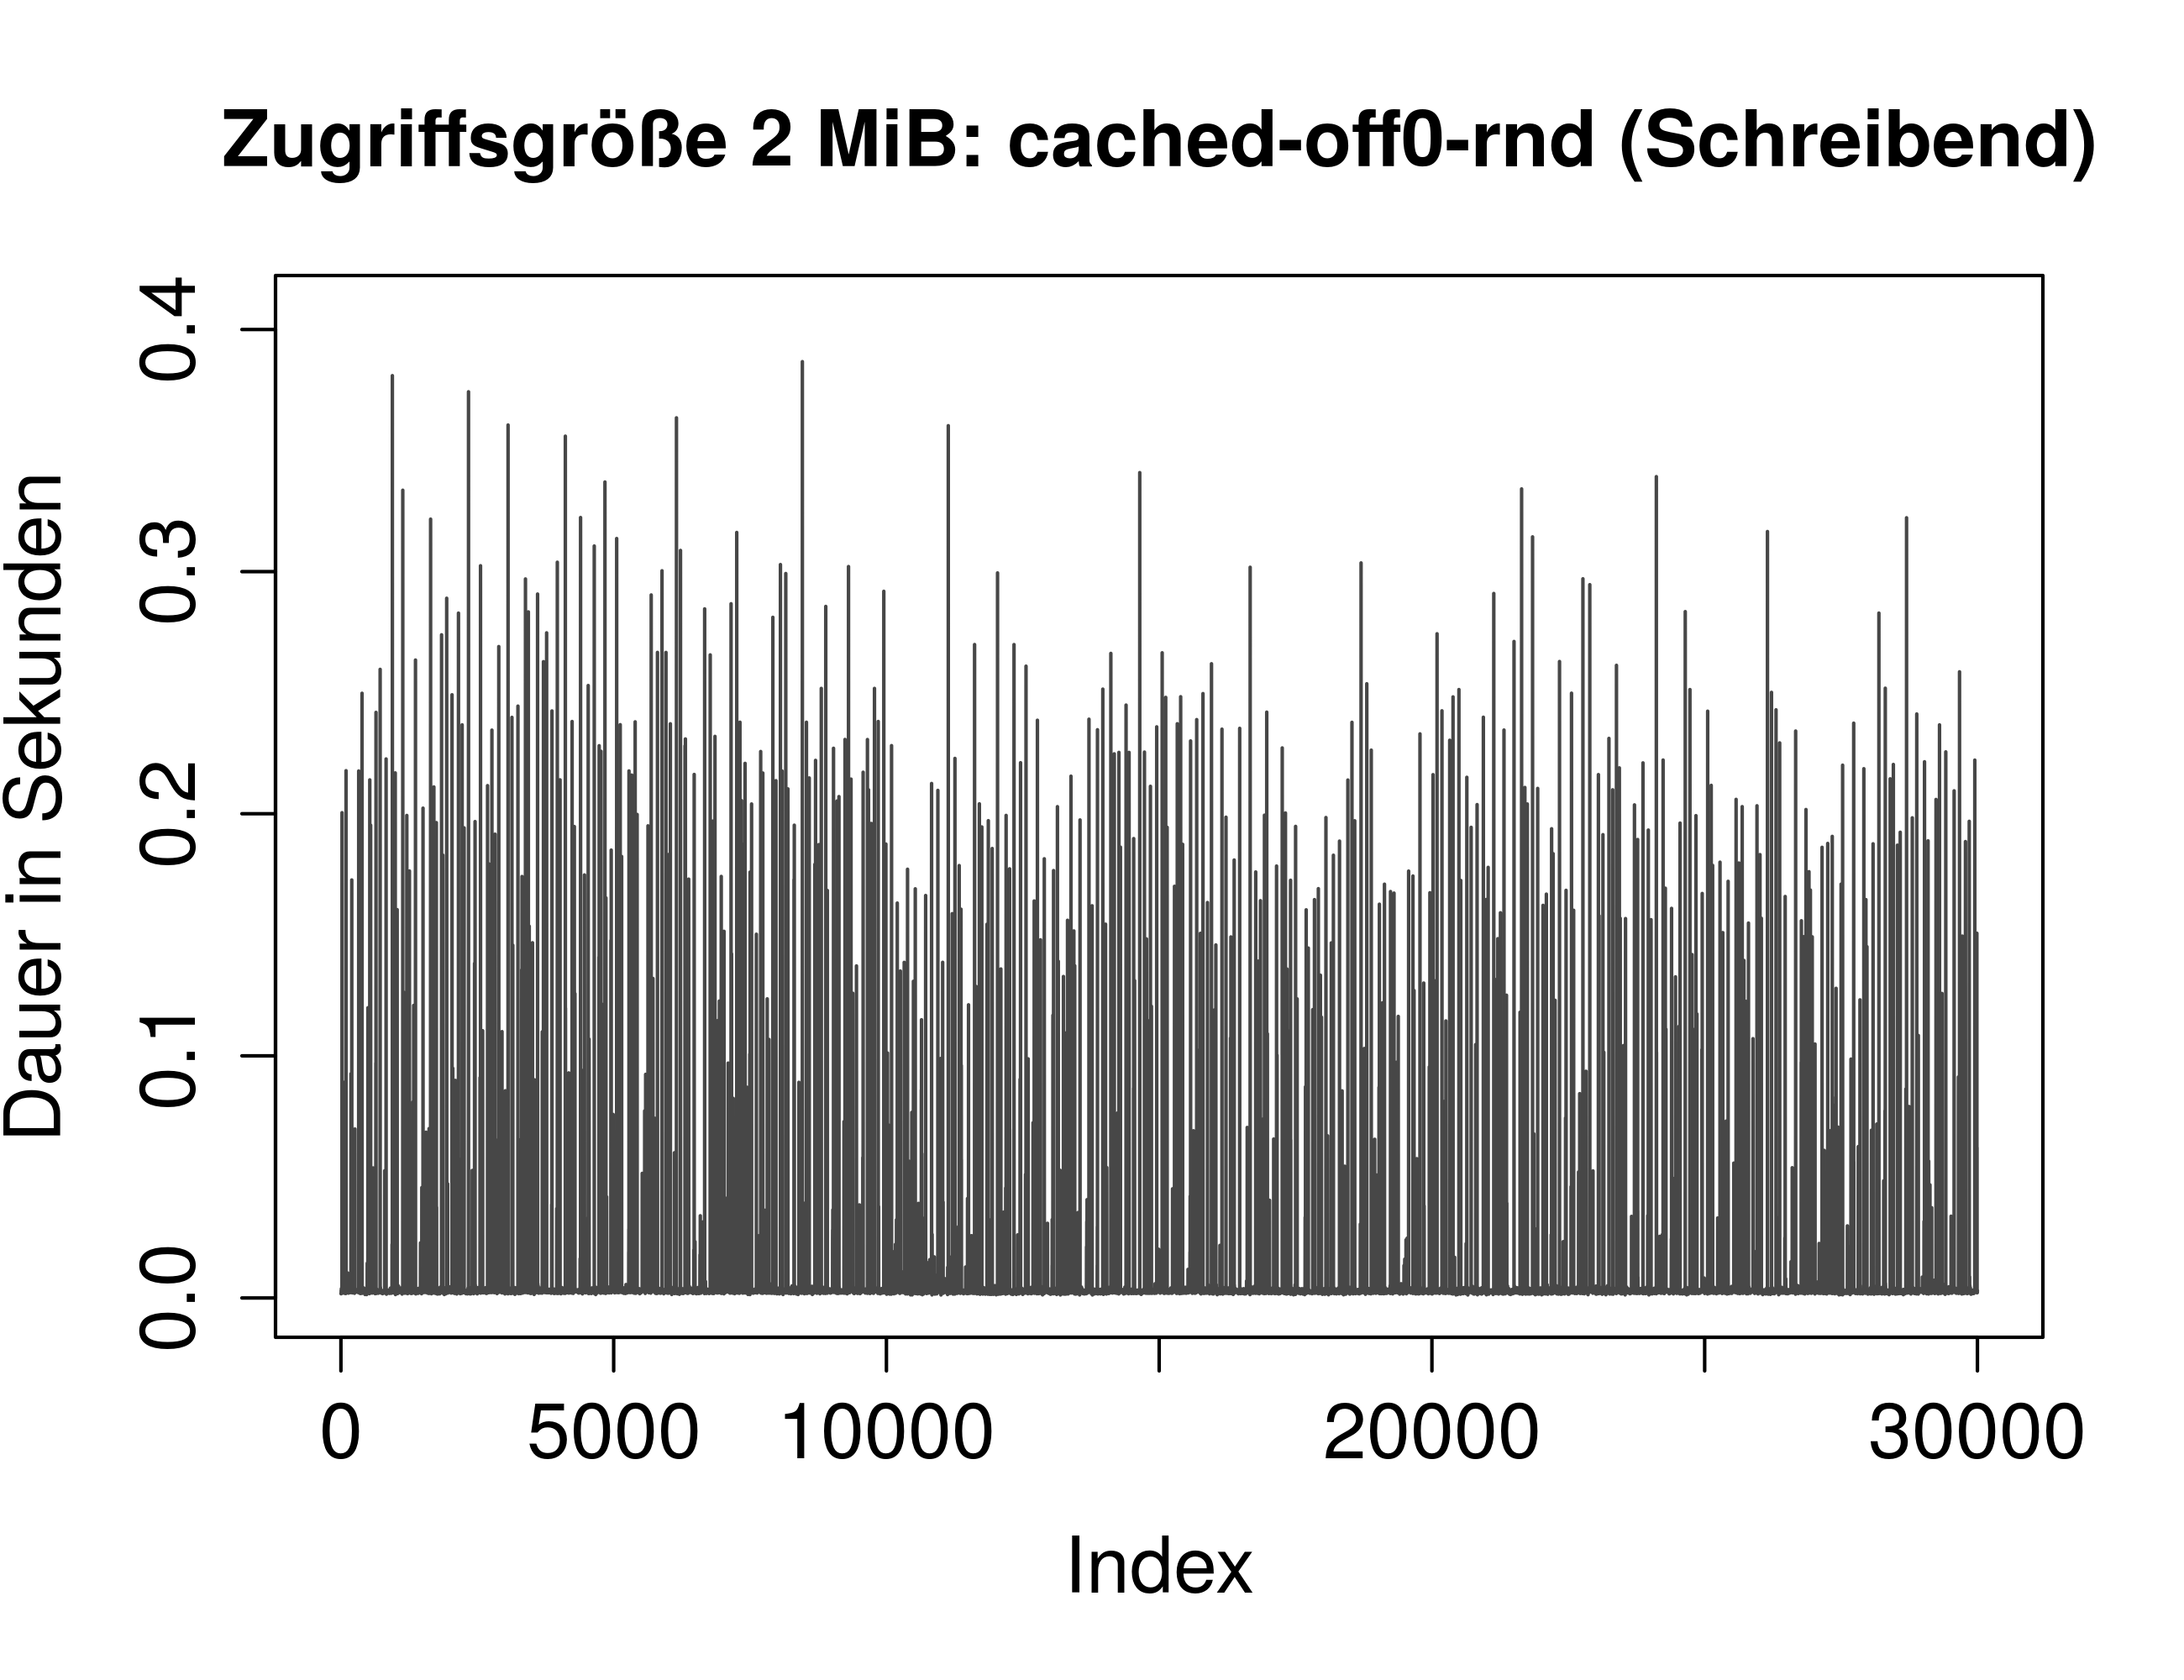
\includegraphics[width=.43\textwidth]{Bilder/Plots/exploration/plot_Size2097152_write_rnd.png}
	}		
	\caption{Detailbetrachtung aller Messungen mit Zugriffsgröße 2097152KB}
	\label{fig:groesse2097152}
\end{figure} 


Um die Messdaten noch detaillierter darzustellen, müssen kleine Ausschnitte herausgegriffen werden. Zunächst betrachte ich die ersten $250$ Messungen. \ref{fig:first250}
Auf den ersten Blick scheint bei cached-off0-seq-W eine gewisse Periodizität ersichtlich (etwa alle 45 Messungen gibt es einen größeren Sprung, alternierend sind die Laufzeiten jeweils etwas langsamer und schneller). Nach genau $123$ Punkten scheint sich das Muster zu wiederholen, dort befindet sich der zweitgrößte Messwert. Wenn man nun als erstes simples Modell eine Fortführung der augenscheinlichen Periodizität der ersten $123$ Messpunkten betrachtet, so erkannt man doch, dass der Verlauf recht unregelmäßig ist. \ref{fig:periodicity} \\
Bei den anderen Graphen kann keine so simple Periodizität vermutet werden.

\begin{figure}
	\subfloat{
		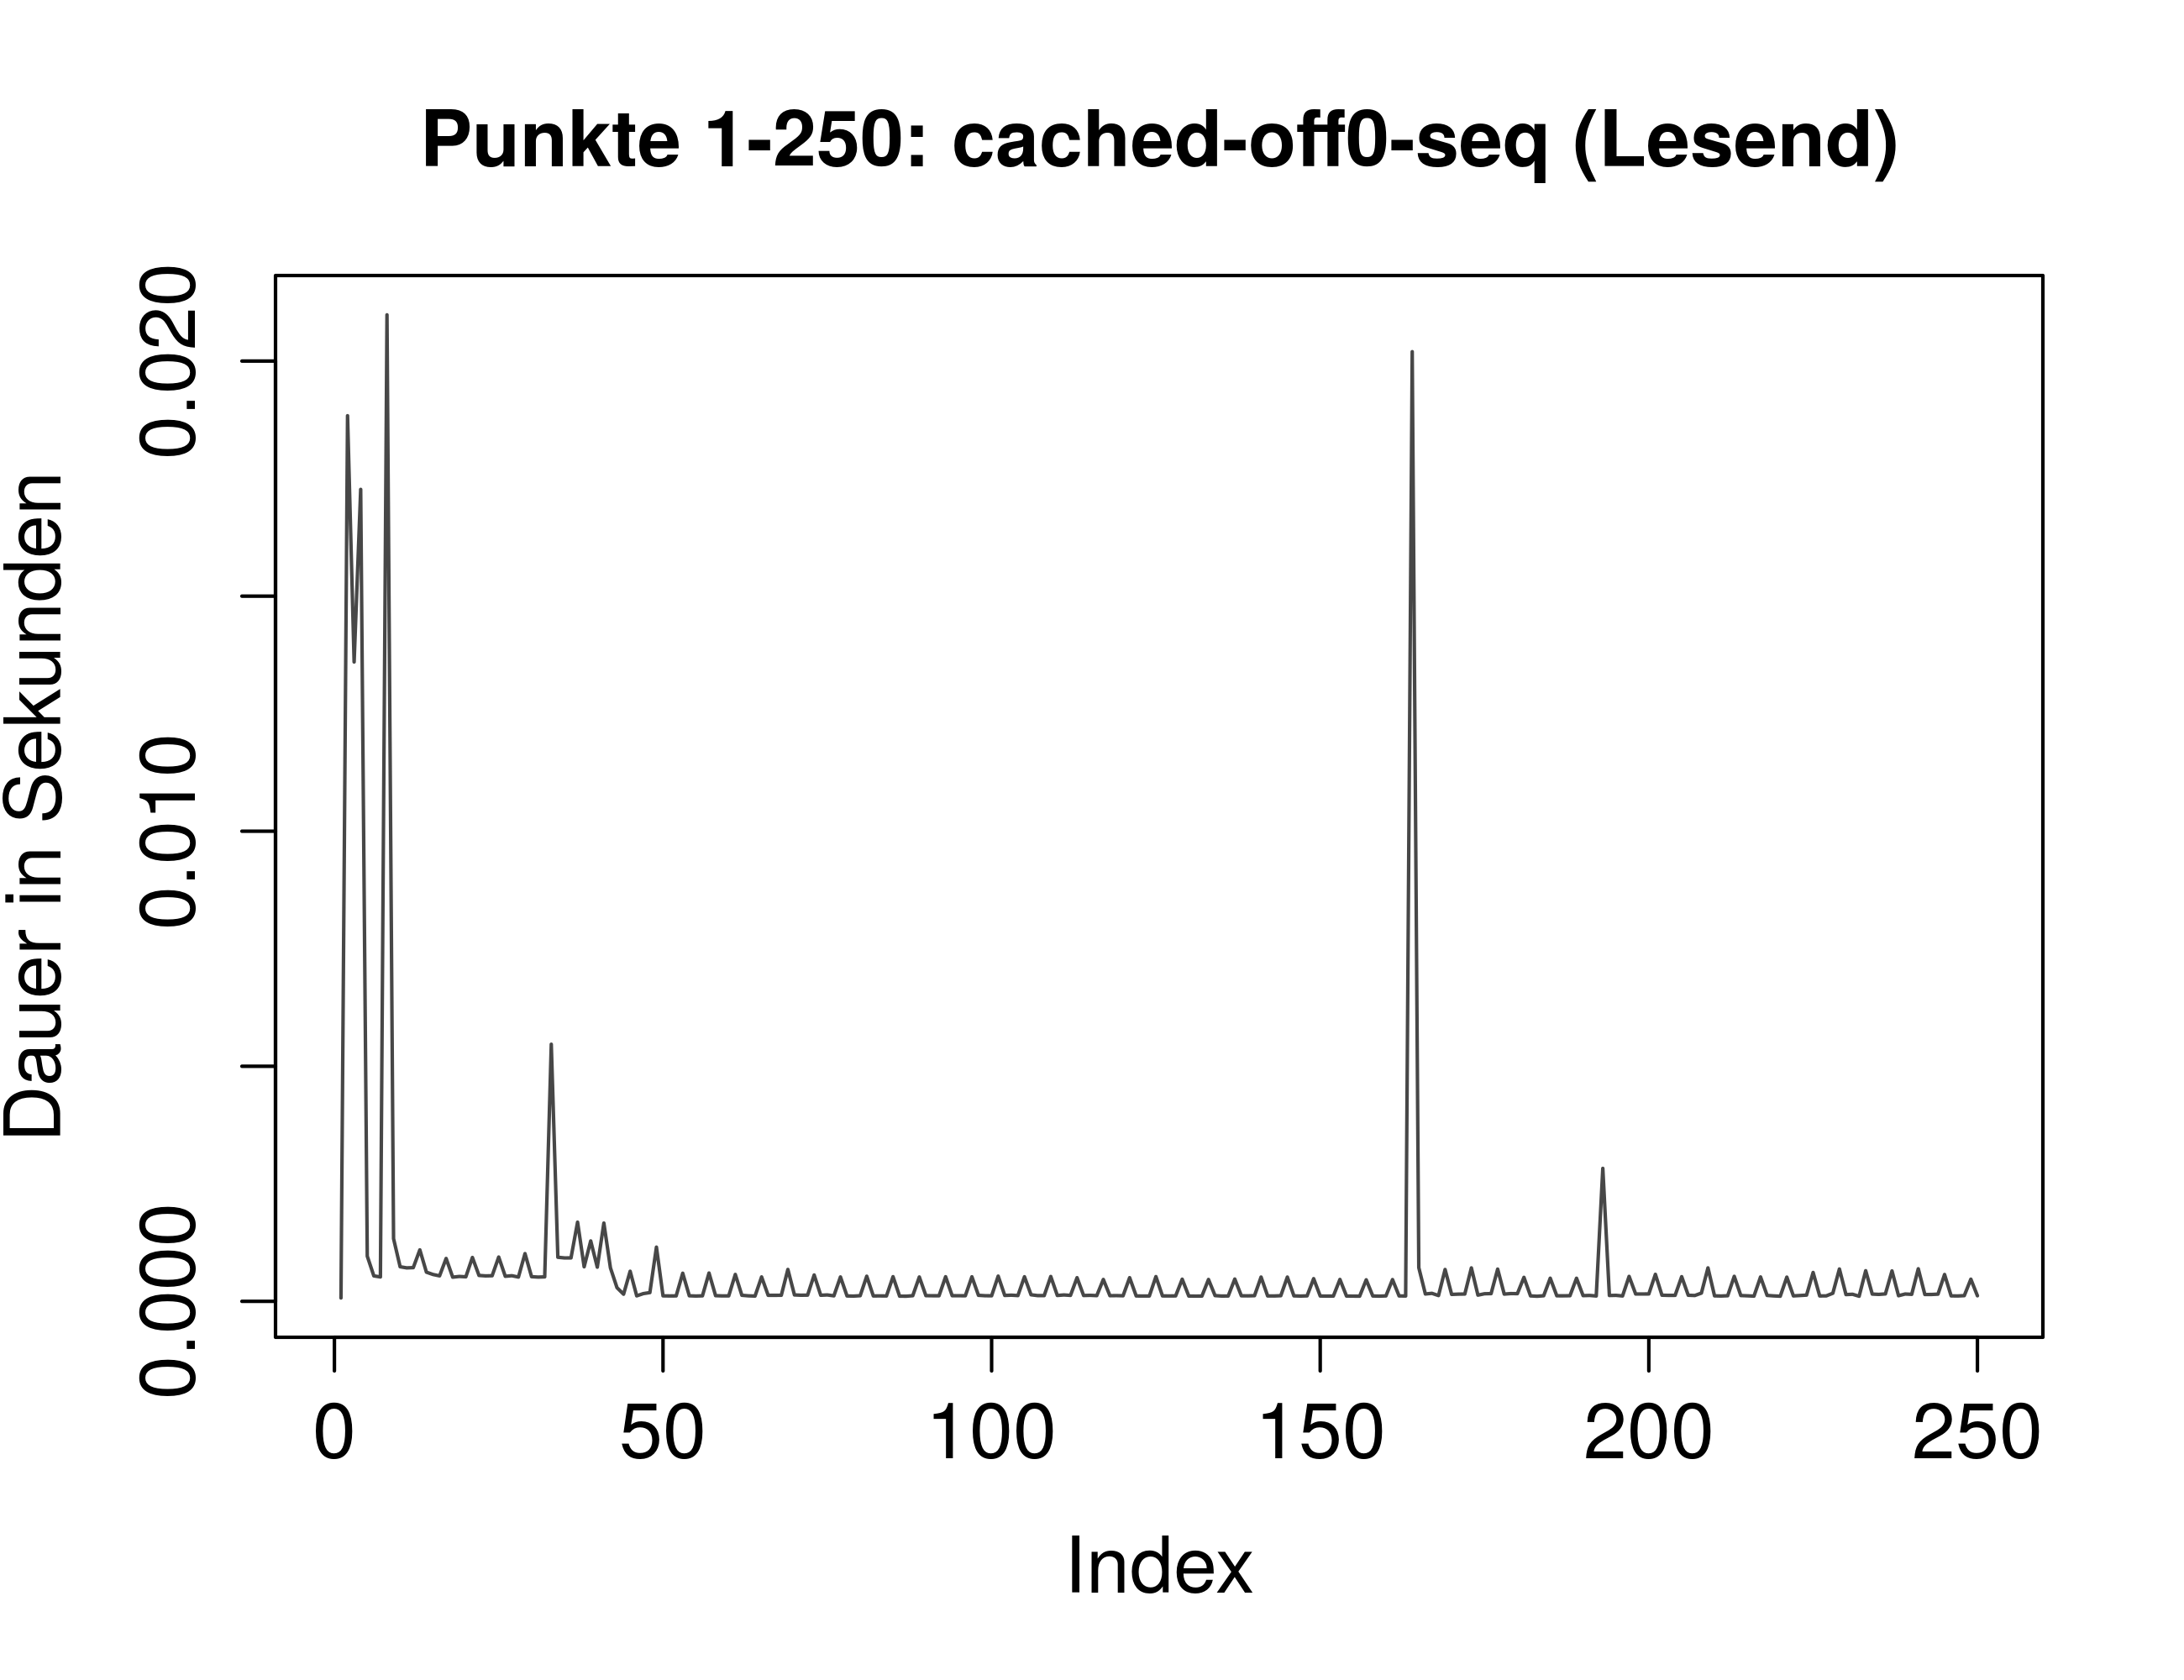
\includegraphics[width=.43\textwidth]{Bilder/Plots/exploration/plot_First250_read_seq.png}
	}
	\hfill
	\subfloat{
		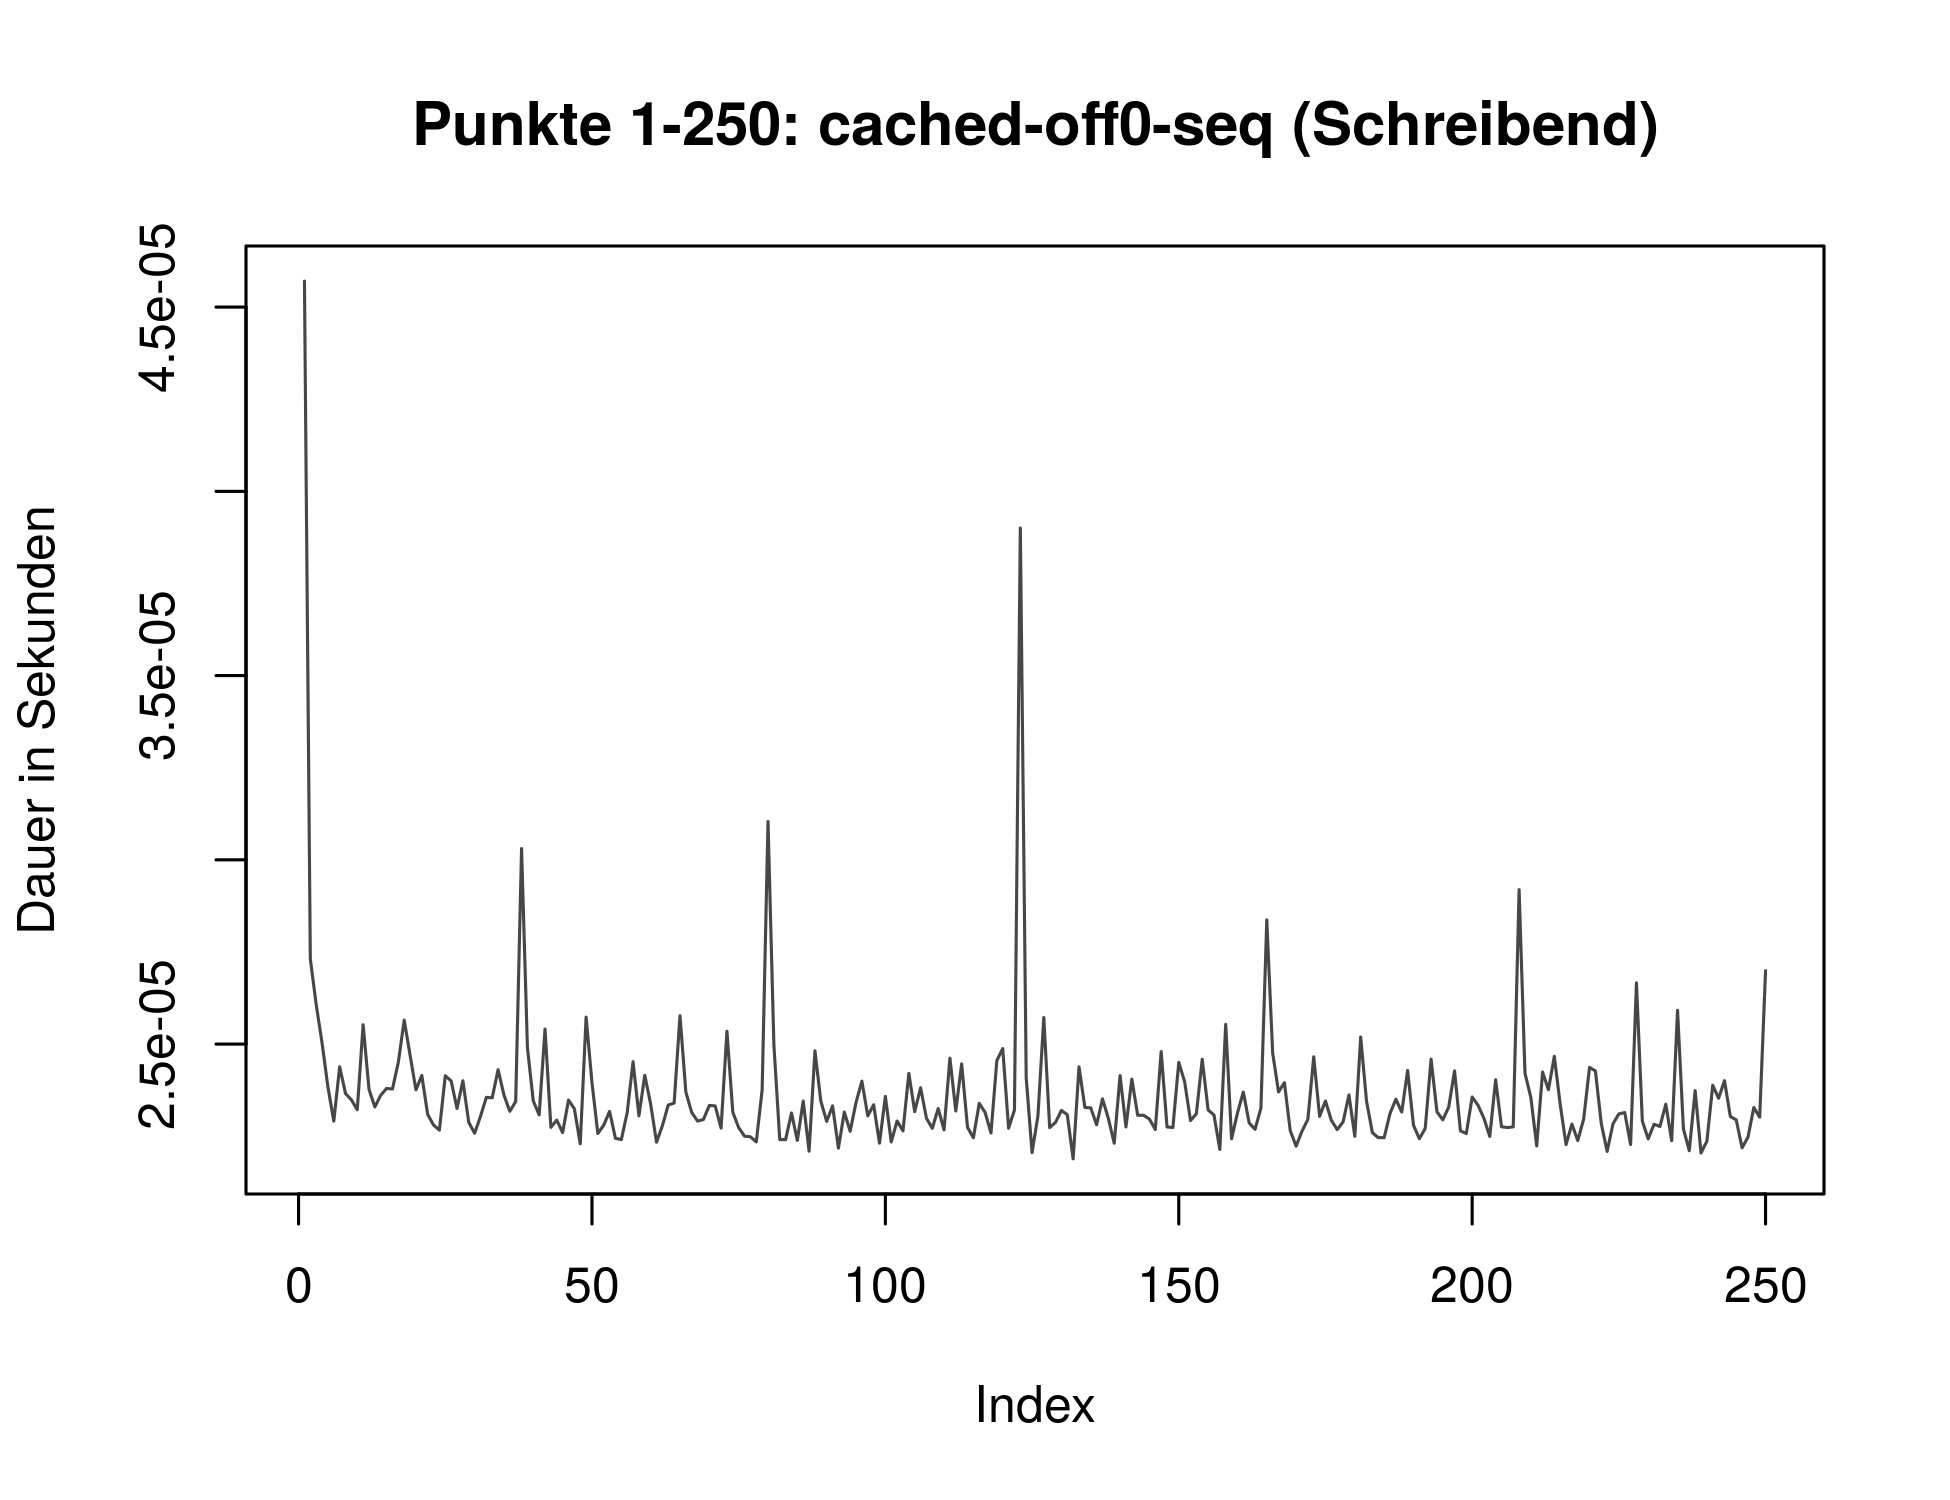
\includegraphics[width=.43\textwidth]{Bilder/Plots/exploration/plot_First250_write_seq.png}
	}\\
	\subfloat{
		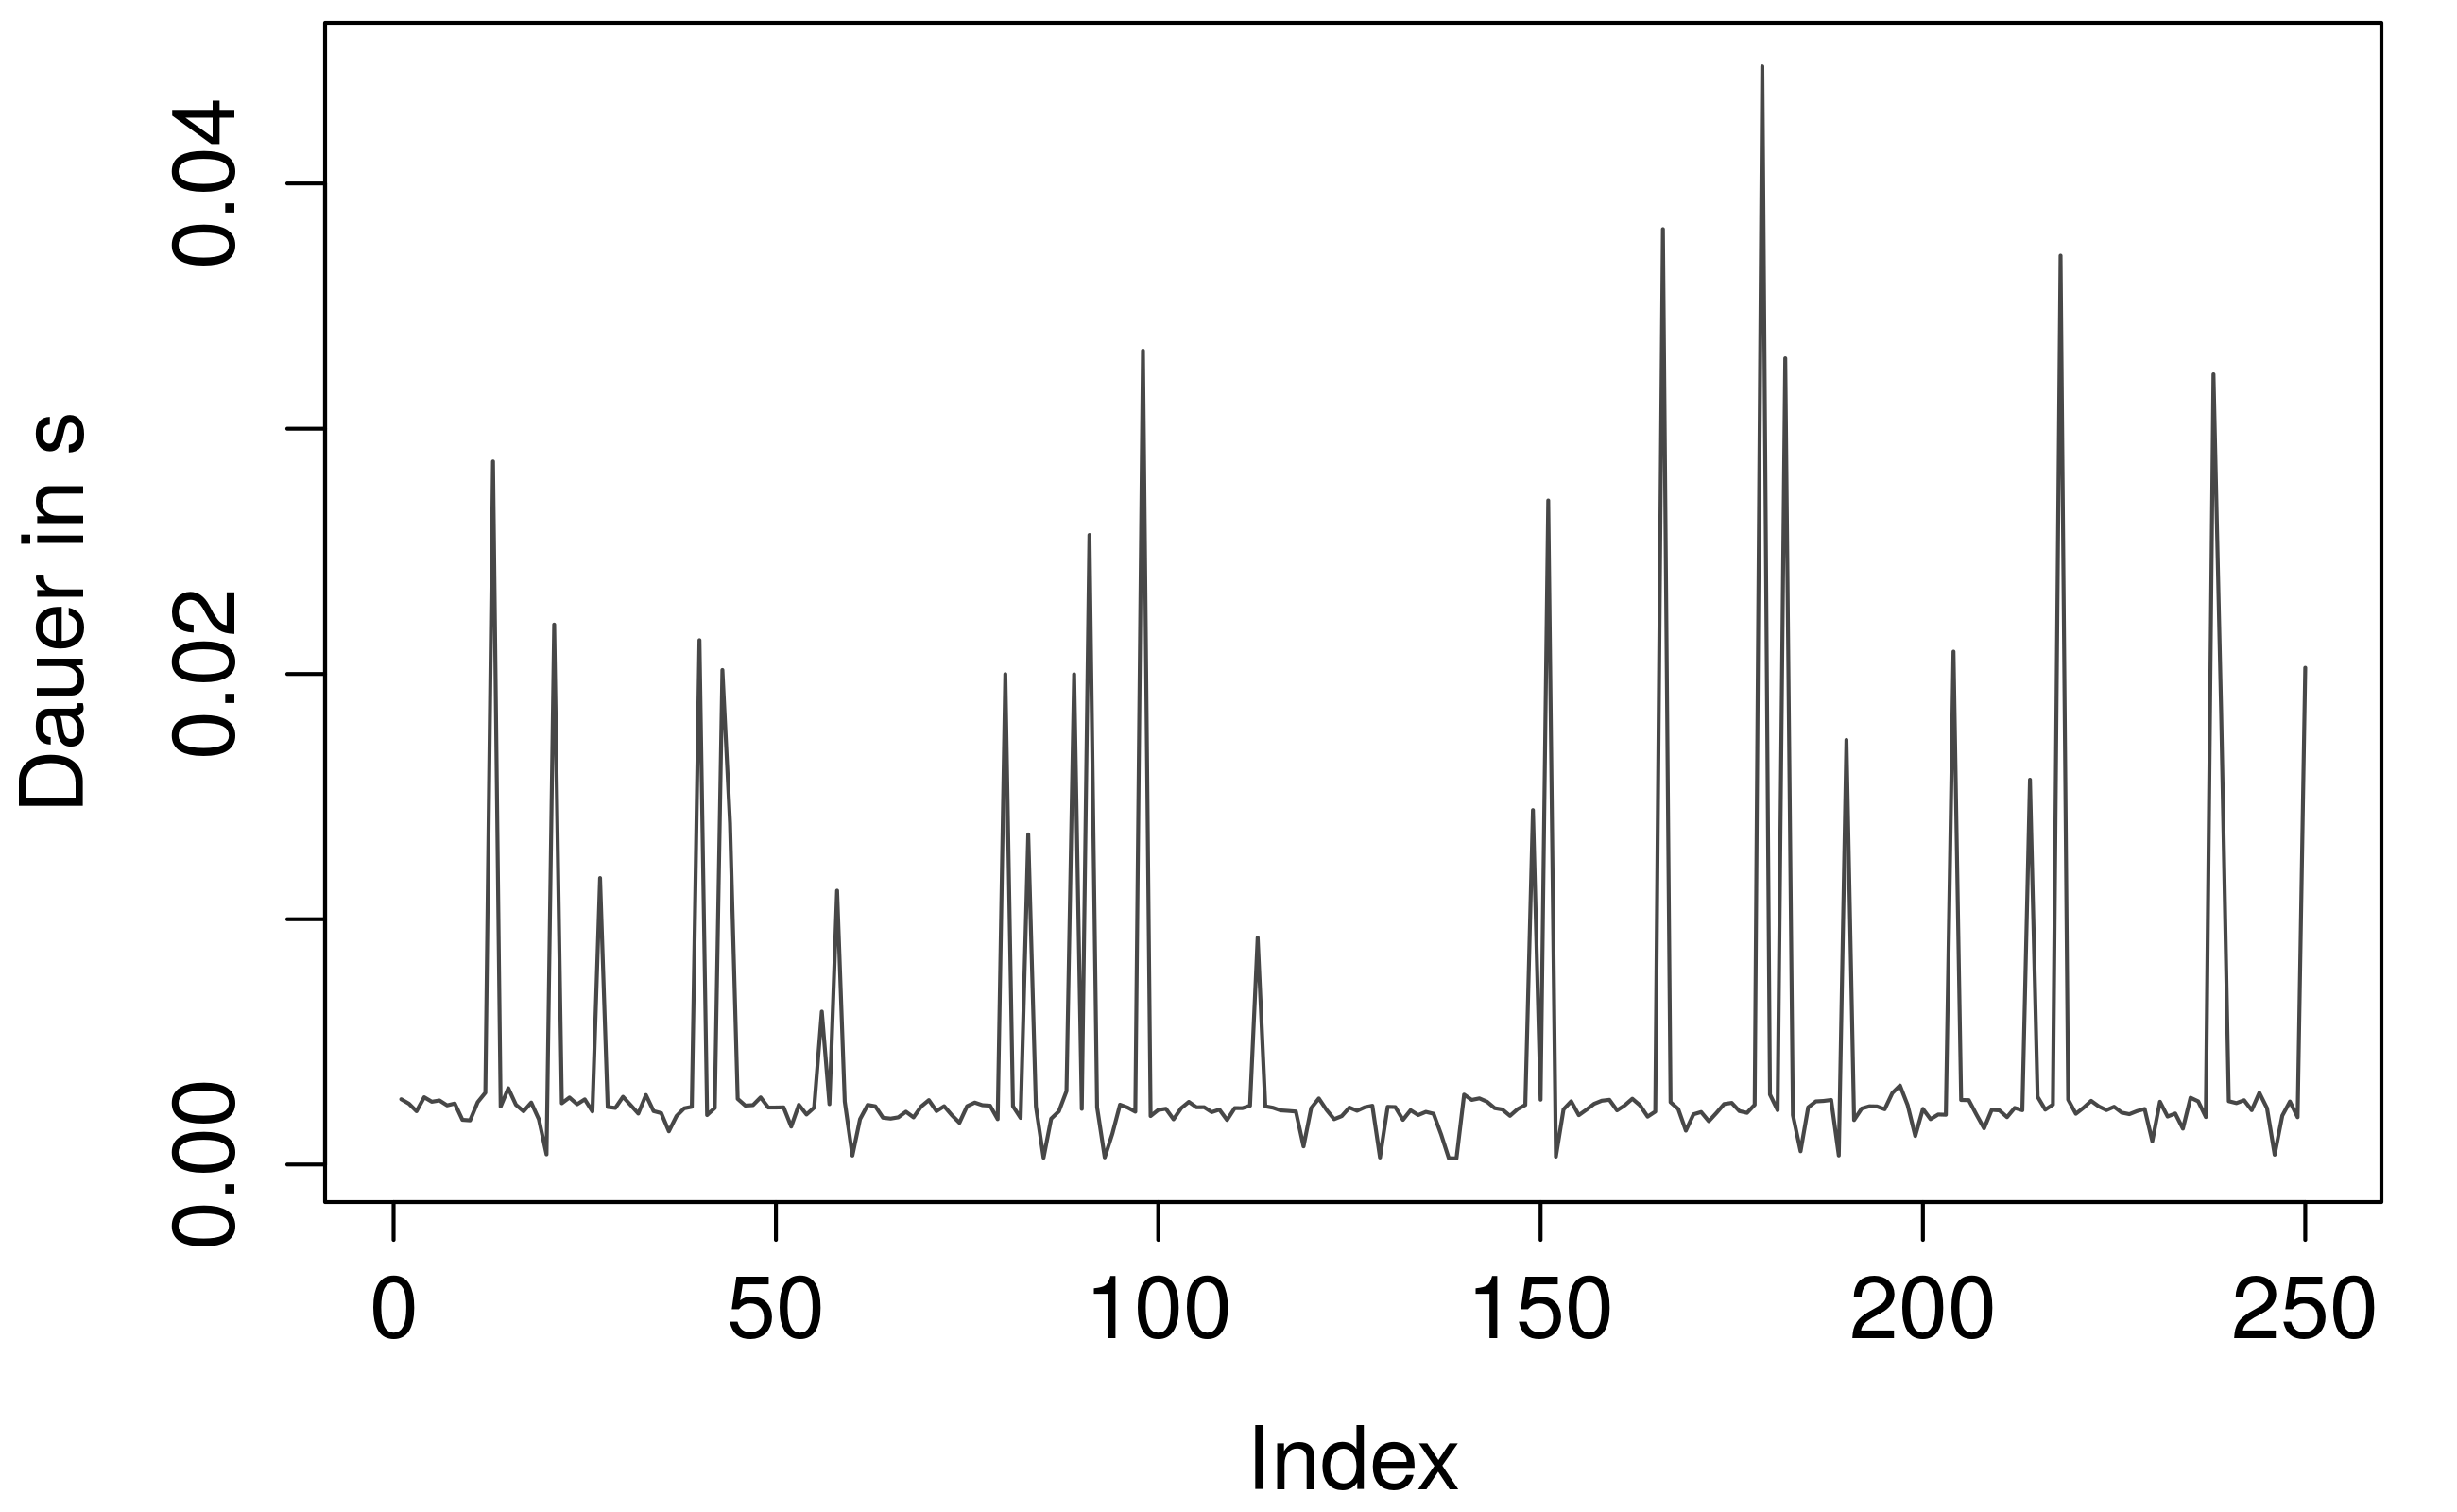
\includegraphics[width=.43\textwidth]{Bilder/Plots/exploration/plot_First250_read_rnd.png}
	}
	\hfill
	\subfloat{
		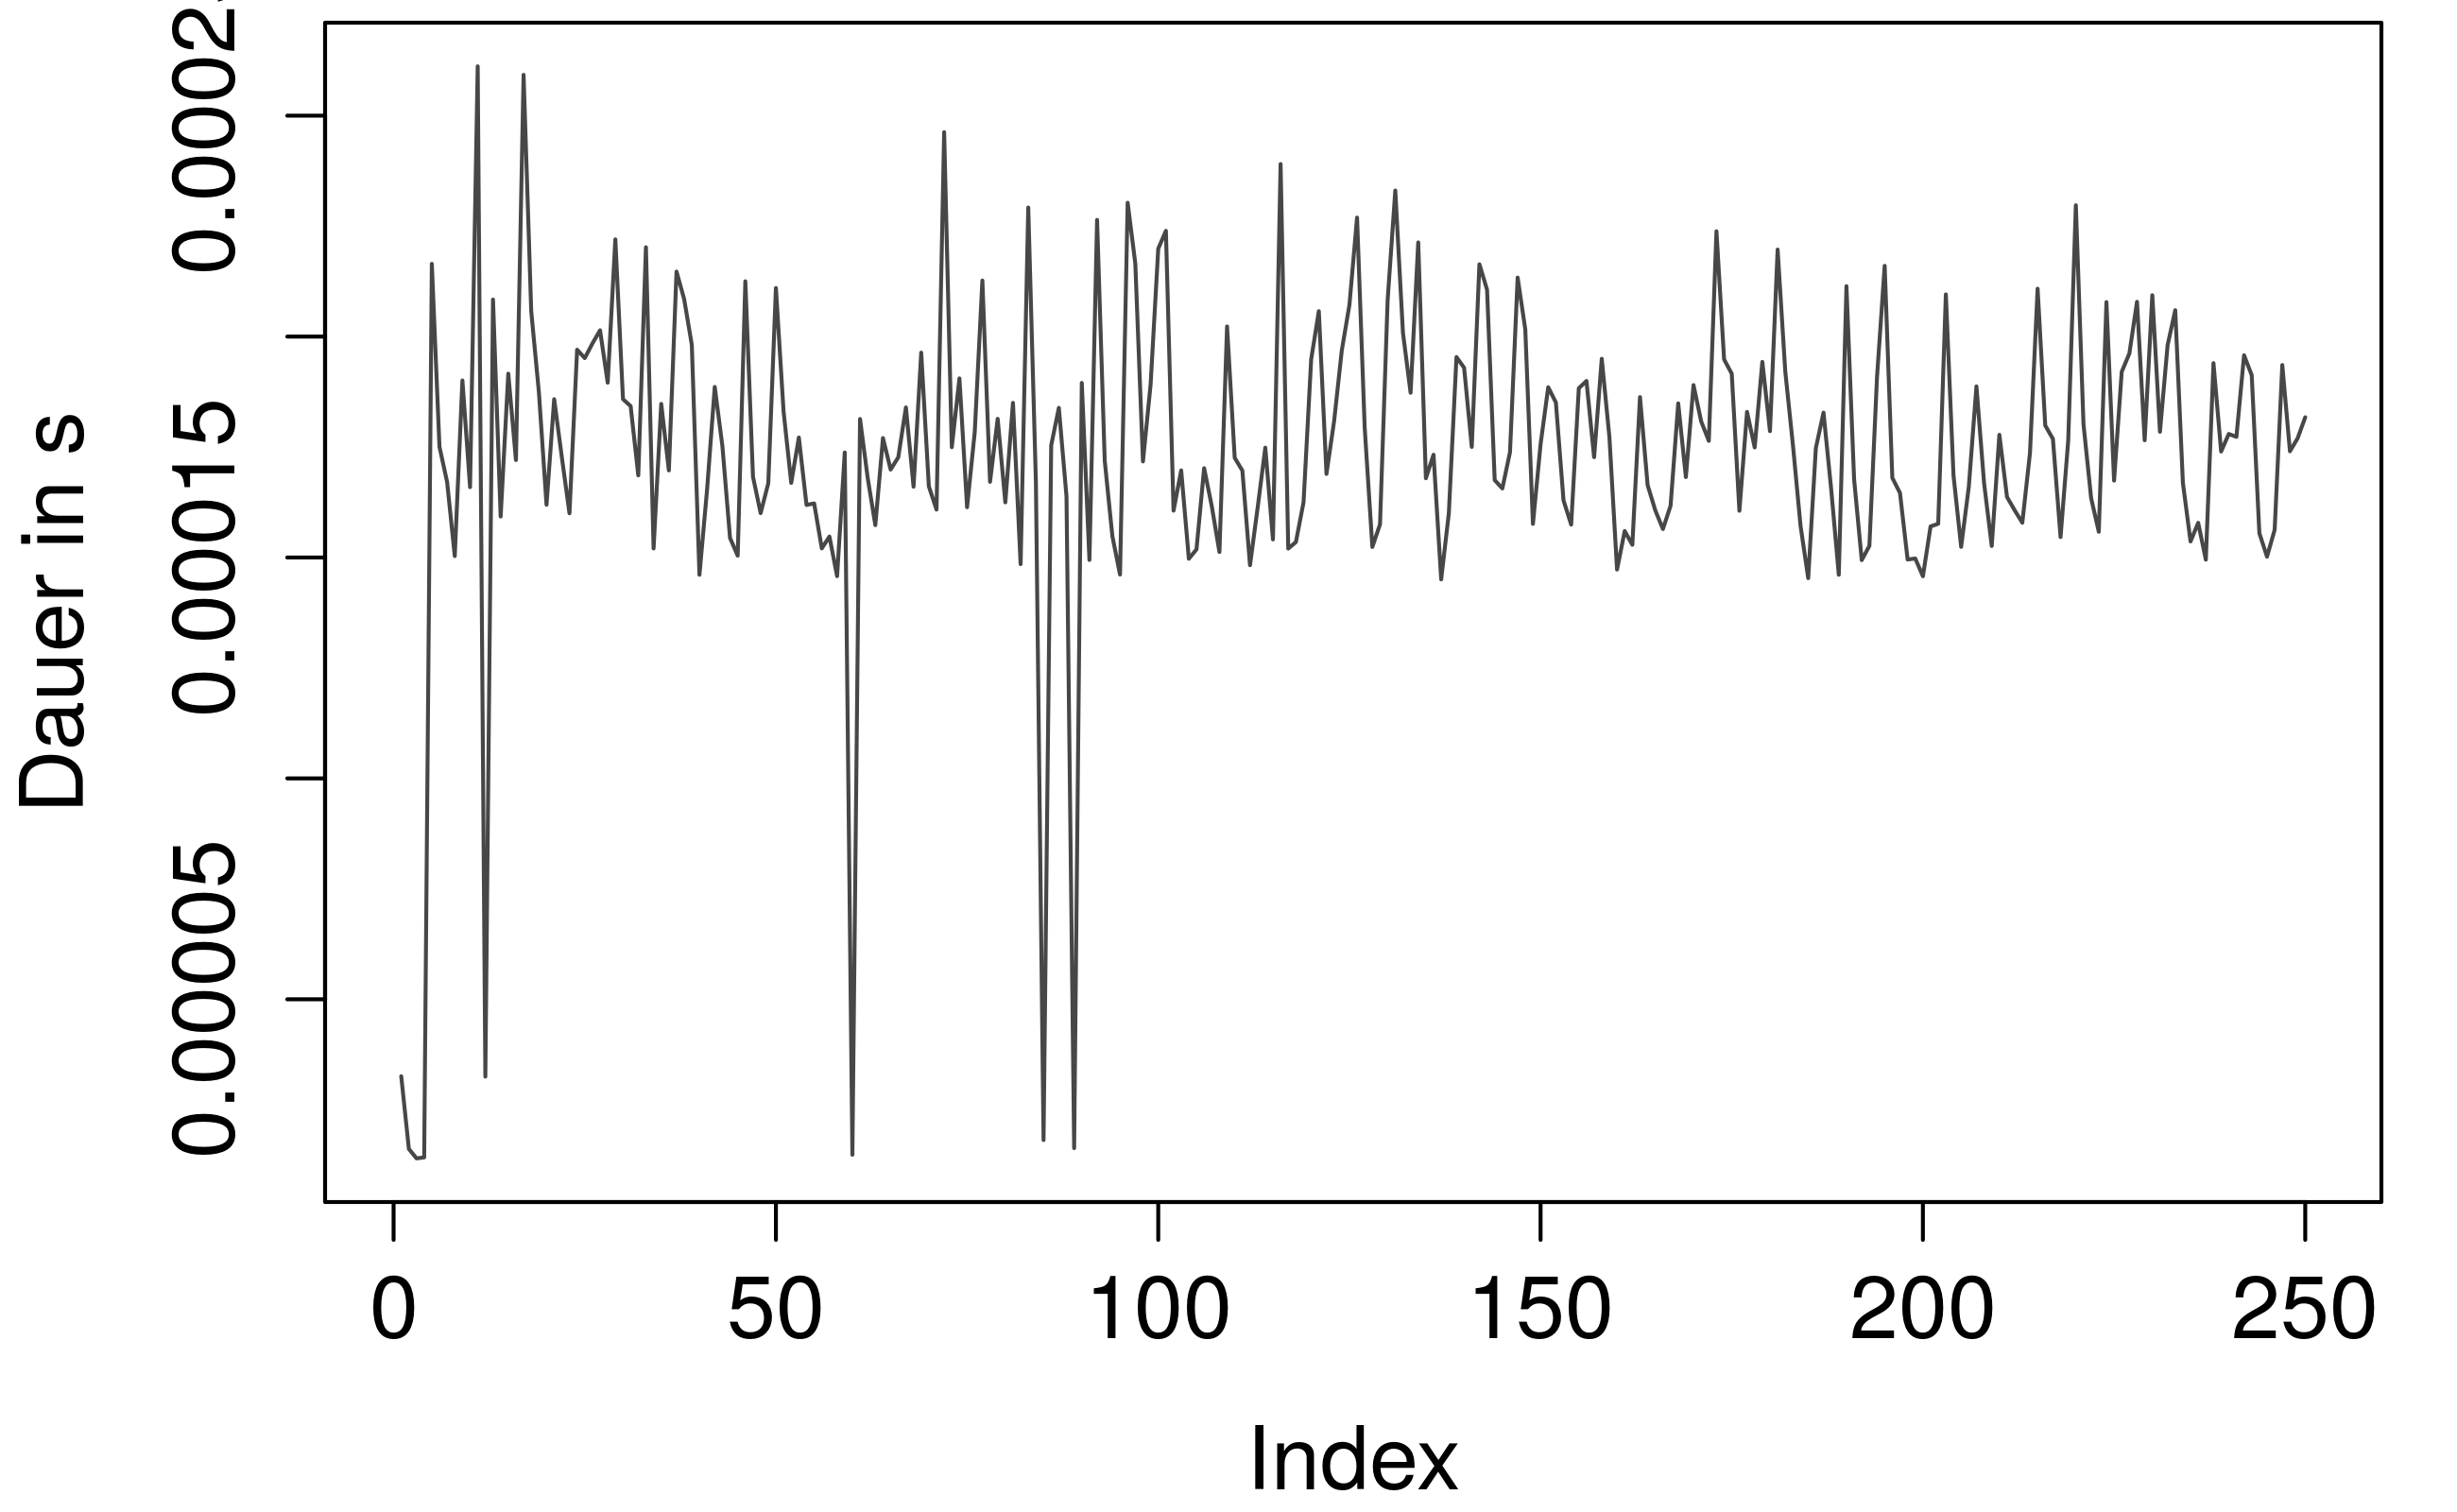
\includegraphics[width=.43\textwidth]{Bilder/Plots/exploration/plot_First250_write_rnd.png}
	}		
	\caption{Detailbetrachtung der ersten 250 Messungen}
	\label{fig:first250}
\end{figure} 

\begin{figure}
	\subfloat{
		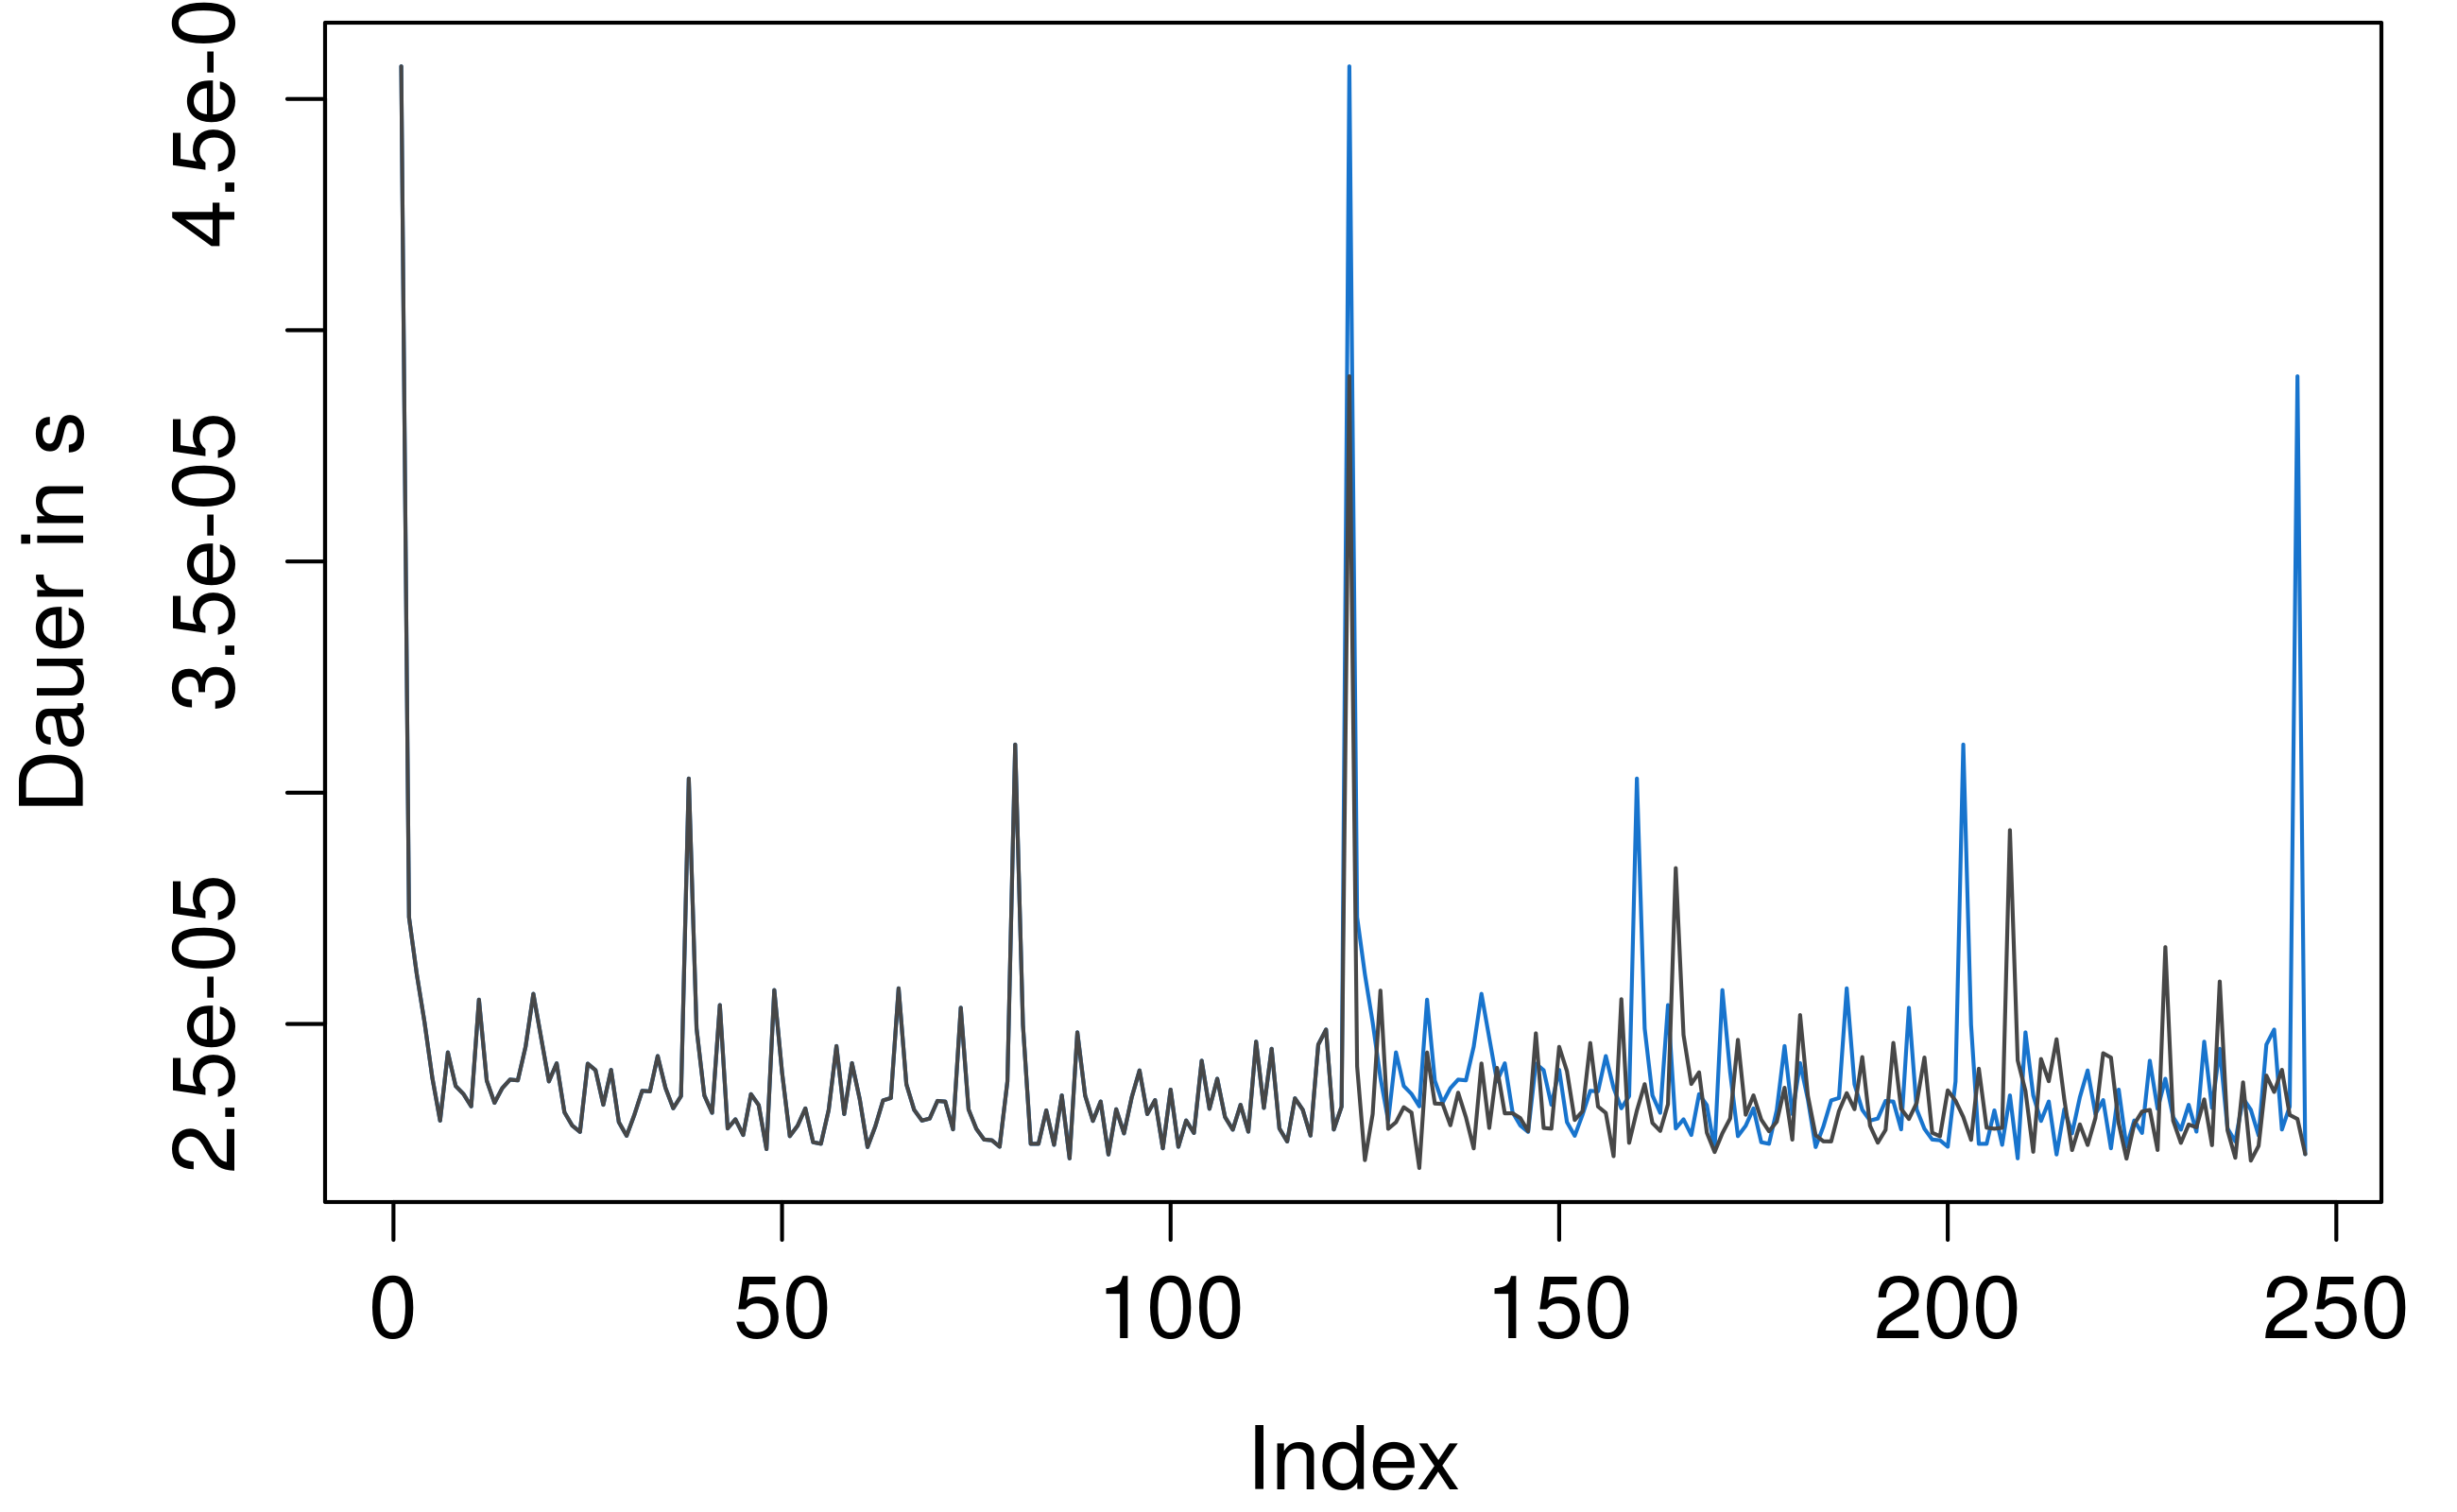
\includegraphics[width=.8\textwidth]{Bilder/Plots/exploration/plot_periodicitywrite_seq.png}
	}	
	\caption{Wiederholung der ersten Werte, als erstes einfaches Modell}
	\label{fig:periodicity}
\end{figure} 

Eine weitere Detailbetrachtung mache ich bei den Messungen 30.001 bis 30.250. \ref{fig:from100001}\\
Hier scheint eine Periodizität bei cached-off0-seq-R vorhanden zu sein. Und wenn eine Überlappung wie zuvor durchgeführt wird (diesmal nach den ersten 129 Messungen), so erkennt man, dass dieses simple Modell die Ausreißer für diesen kleinen Ausschnitt exakt vorhersagen kann. \ref{fig:periodicity100001}\\
Im Allgemeinen kann dies jedoch offensichtlich nicht funktionieren. Doch unsere Annahme \textbf{ABSCHNITT} einer gewissen Periodizität in der Leistung des E/A-Systems ist scheinbar gerechtfertigt. Ein Modell das versucht diese auszunutzen muss eine komplexere Methode als schlichtes Übertragen vorheriger Leistungswerte haben, ansonsten kann es wohl nur in äußerst eingeschränktem Maße korrekte Leistung vorhersagen.

\begin{figure}
	\subfloat{
		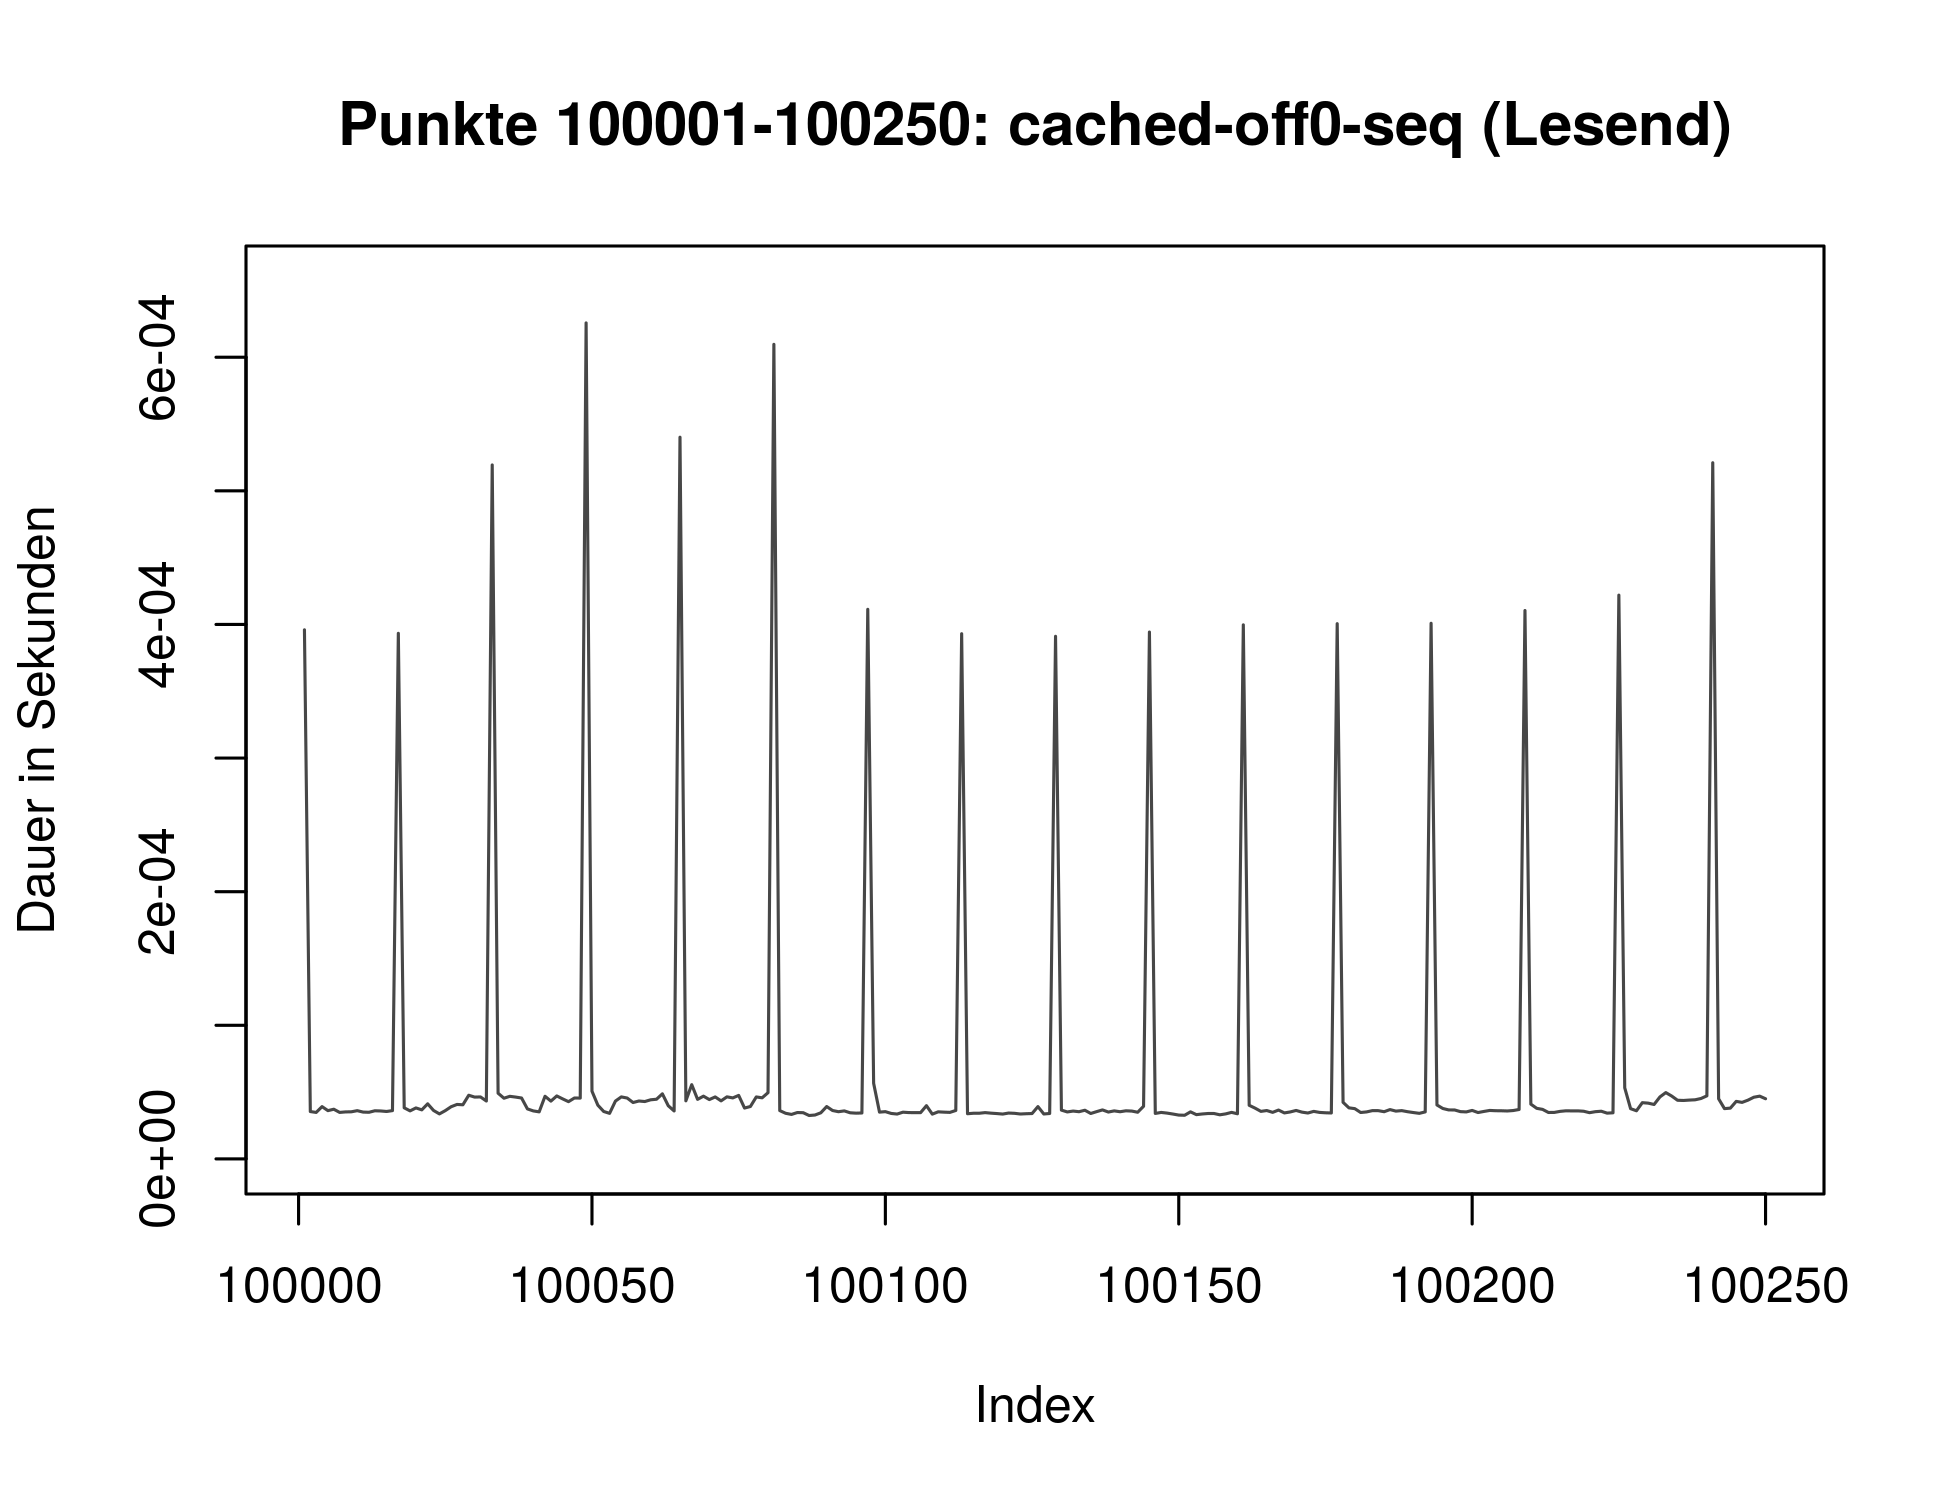
\includegraphics[width=.43\textwidth]{Bilder/Plots/exploration/plot_From100001to100250_read_seq.png}
	}
	\hfill
	\subfloat{
		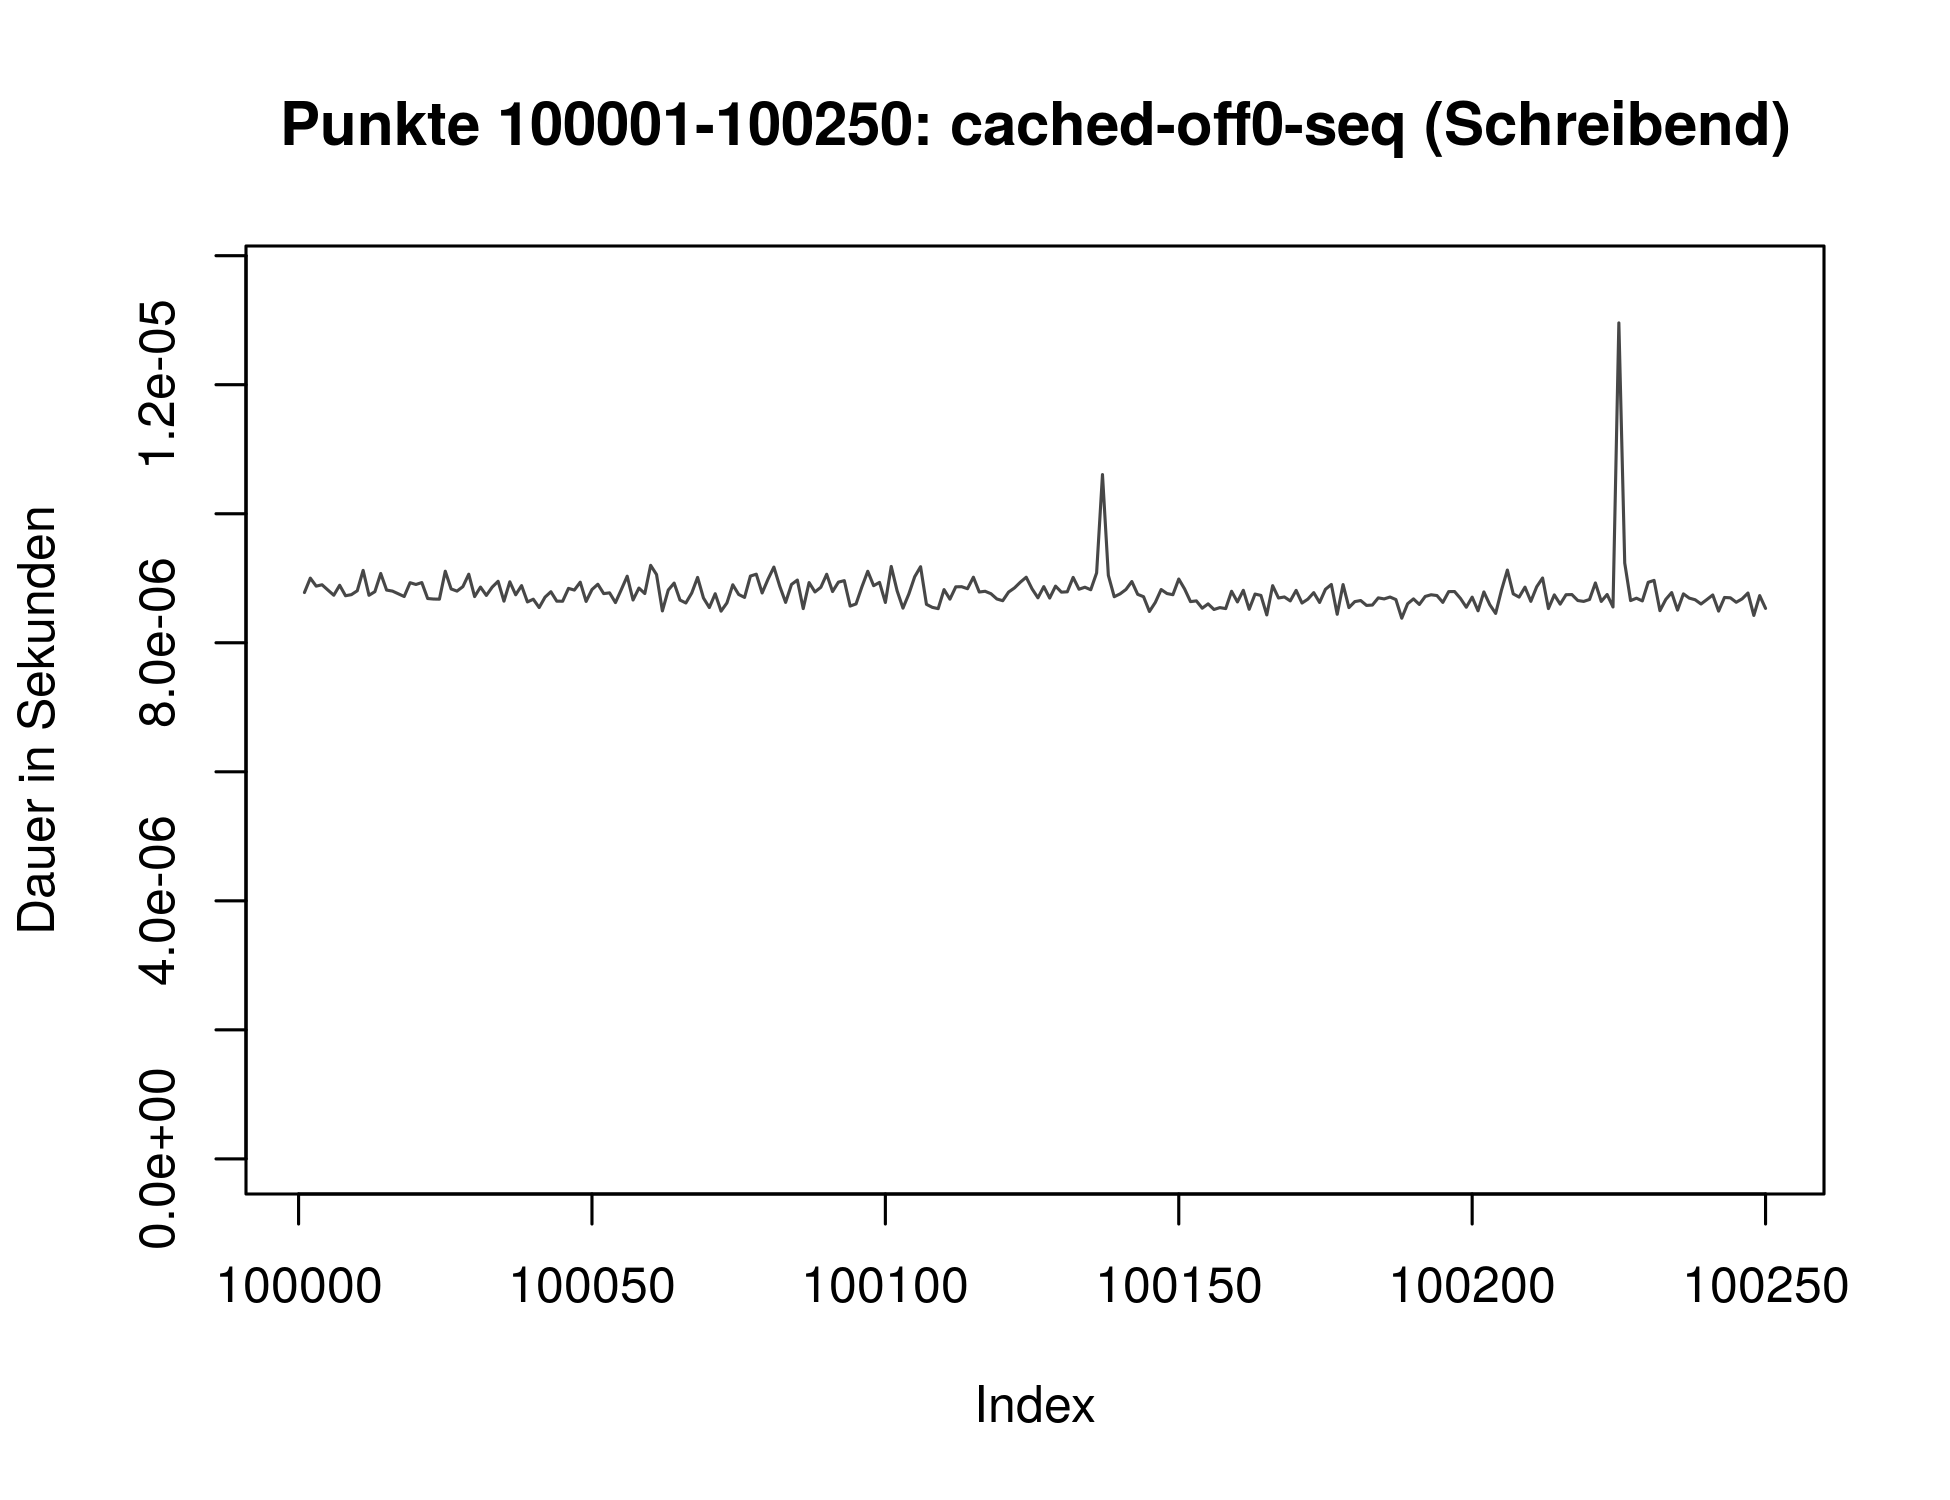
\includegraphics[width=.43\textwidth]{Bilder/Plots/exploration/plot_From100001to100250_write_seq.png}
	}\\
	\subfloat{
		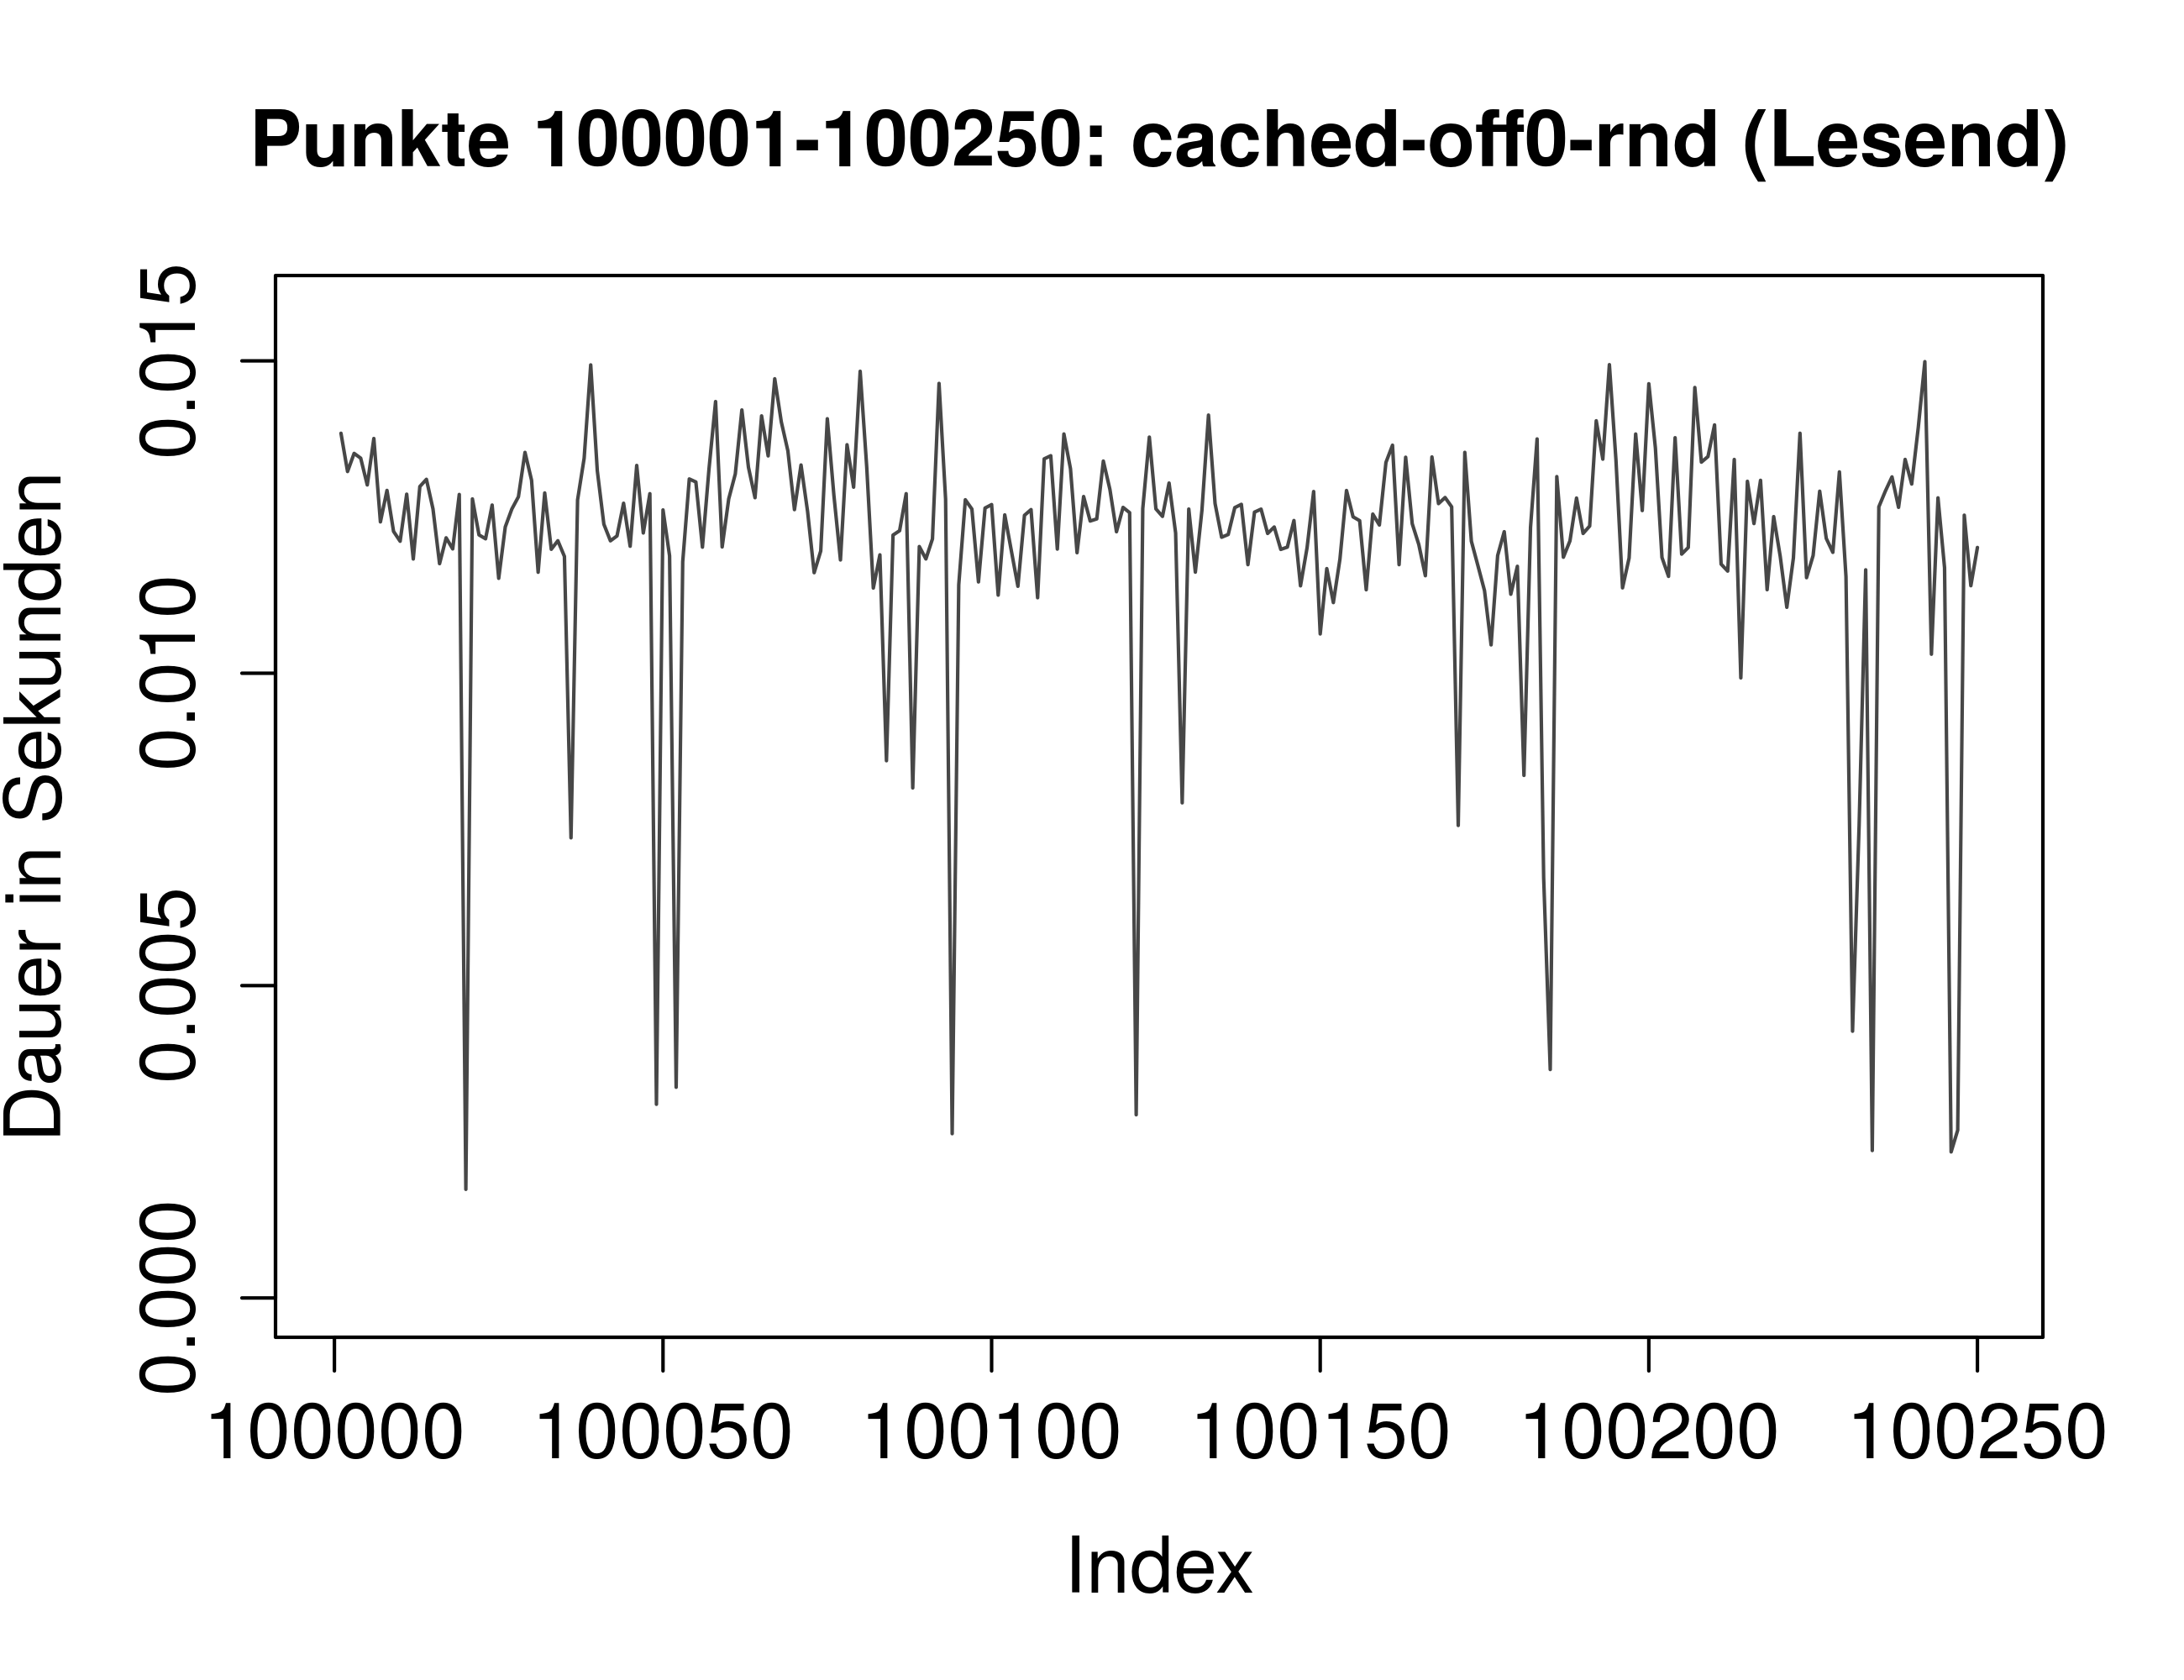
\includegraphics[width=.43\textwidth]{Bilder/Plots/exploration/plot_From100001to100250_read_rnd.png}
	}
	\hfill
	\subfloat{
		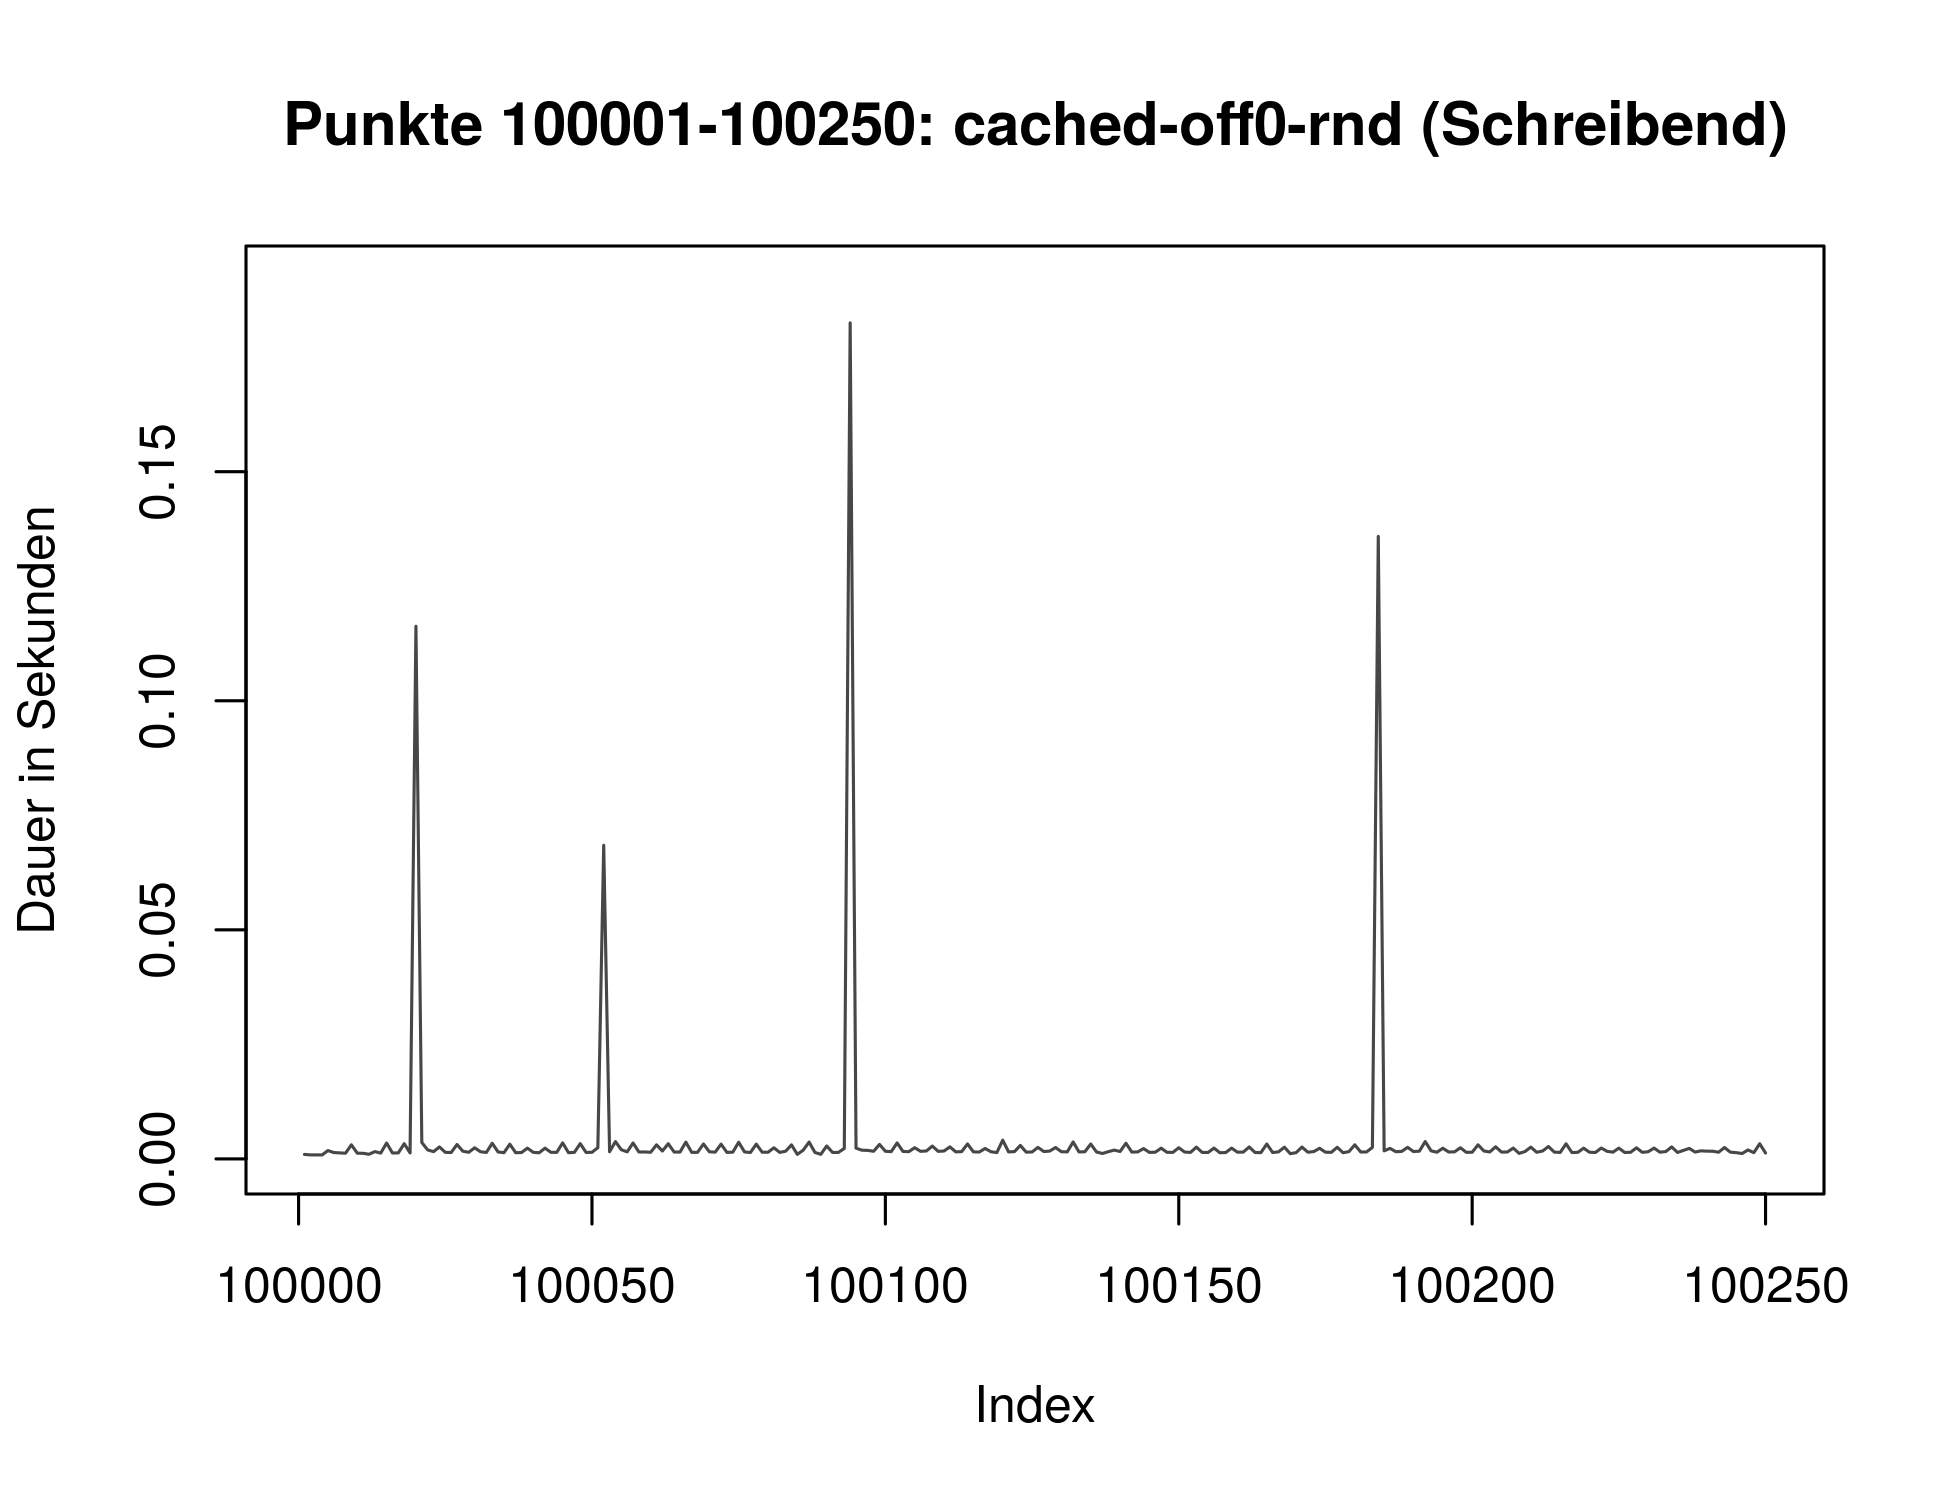
\includegraphics[width=.43\textwidth]{Bilder/Plots/exploration/plot_From100001to100250_write_rnd.png}
	}		
	\caption{Detailbetrachtung der Messungen 100001 bis 100250}
	\label{fig:from100001}
\end{figure} 

\begin{figure}
	\subfloat{
		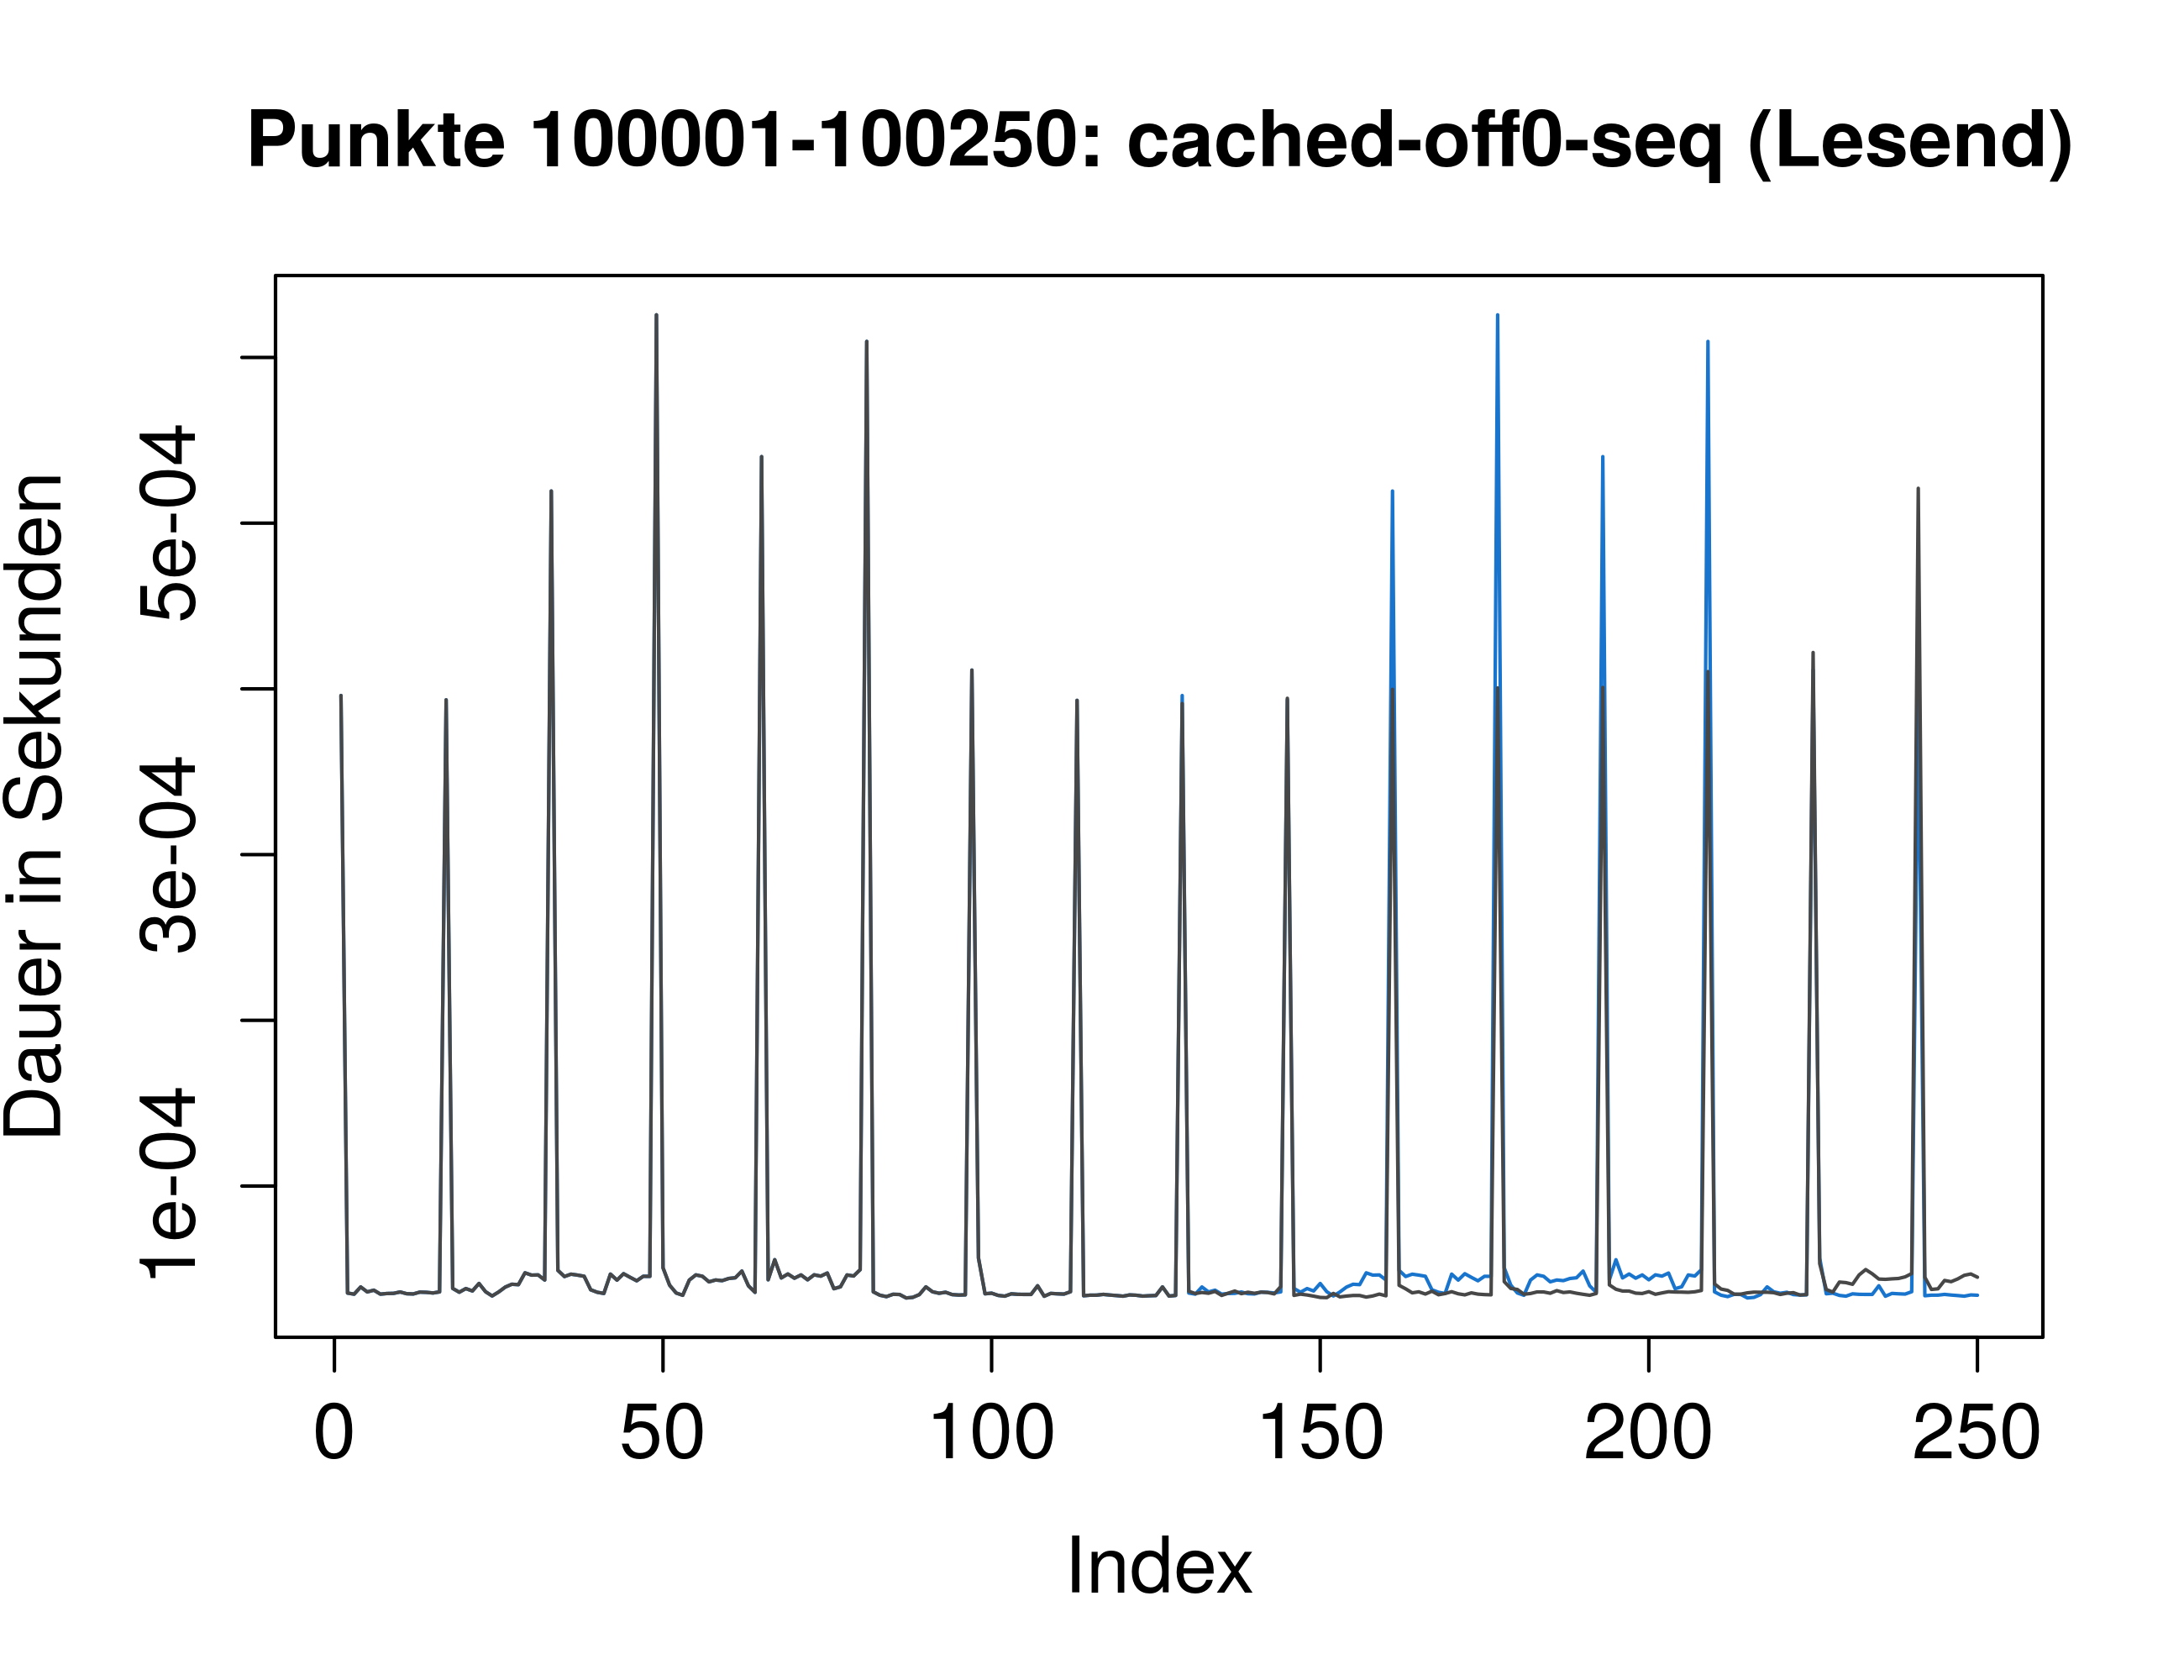
\includegraphics[width=.8\textwidth]{Bilder/Plots/exploration/plot_periodicity100001read_seq.png}
	}	
	\caption{Wiederholung der ersten Werte, als erstes einfaches Modell}
	\label{fig:periodicity100001}
\end{figure} 

\section{Analyse der Fehlerklassen}

Die in \textbf{VERWEIS} eingeführten Fehlerklassen untersuche ich anhand der Ergebnisse, die aus der Clusteranalyse des Fehlers von LinReg G entstanden sind.
In \ref{fig:error_class_clustering_seq} a), sowie \ref{fig:error_class_clustering_rnd} a) ist in Zeitreihe der Fehler aufgezeichnet, den LinReg G auf cached-off0-seq, bzw cached-off0-rnd, mit seinen Vorhersagen gegenüber den tatsächlichen Laufzeiten gemacht hat. In \ref{fig:error_class_clustering_seq} c) und \ref{fig:error_class_clustering_rnd} c) ist das gleiche gezeichnet, allerdings sind die größten und kleinsten Werte weggelassen. Dabei können auf dem Graph zum sequentiellen Datensatz Phasen mit guten und schlechten Vorhersagen erkannt werden. Hier wird ein Verhalten visualisiert, das darauf rückschließen lässt, dass das Modell die Laufzeiten mancher Attribut-Sets besser modelliert hat, als das von anderen. Denn hier wird das selbe Attribut-Set vielfach hintereinander getestet. Der Dateizugriffsort ändert sich bei jedem Zugriff auf dem randomisierten Datensatz und entsprechend ist dieses Verhalten hier nicht so stark ausgeprägt. Auf diesem Datensatz ist dagegen eine unterschiedlich gute Modellierung für Lese- und Schreibzugriffe erkennbar, denn die erste Hälfte der Fehler hat einen flacheren und gleichmäßigeren Verlauf, als die zweite Hälfte, in der die schreibenden Messungen sichtbar sind. \textbf{LÜCKE RECHTs}
In den Graphen jeweils rechts neben den beschriebenen ist durch farbliche Markierung die Zugehörigkeit der Messpunkte zu den unterschiedlichen Klassen erkennbar. Die Unterscheidung in verschiedene Klassen findet in horizontalen Linien statt. Eine Klasse deckt einen bestimmten Bereich der Fehlerwerte ab, die abgedeckten Bereiche lassen sich aus \ref{tab:error_classes_switched} entnehmen. 
Bei der Betrachtung der Graphen mit nach Fehler sortierten Punkten ( \ref{fig:error_class_clustering_seq} e) und f), sowie \ref{fig:error_class_clustering_rnd} e) und f) ) können die Anzahlen der jeweils zugeordneten Punkte zu den Klassen gut quantifiziert werden (die exakten Zahlen sind auch \ref{tab:error_classes_switched} zu entnehmen). In beiden Fällen enthält eine Klasse den Großteil der Punkte (jeweils etwa $3/4$), die Klassen, dessen Bereich leicht abweichen, enthalten noch einen kleinen Anteil der Messdaten. Die Ausreißer in beide Richtungen machen quantitativ fast nichts aus, werden allerdings durch mehrere Klassen abgedeckt. So werden die obersten \textbf{WERT} \% der Daten auf cached-off0-rnd in 6 Klassen aufgeteilt.\\
Das Modell scheint generell schon recht gut zu sein, da die Fehler sich für die Klassen mit dem kleinsten durchschnittlichen Fehler sammeln. Es gibt allerdings einige Datenpunkte, die das Modell sehr schlecht vorhersagen konnte. Die Annahme ist nun, dass die voneinander stark abweichenden Datenpunkte grundsätzlich unterschiedlich vom System verarbeitet wurden. Sodass die Fehlerklassen die unterschiedlichen E/A-Wege im System repräsentieren. 
Ein Modell, dass eine Modellierung mit dem zusätzlichen Wissen dieser Klassenzuordnungen vornimmt, sollte die Ausreißer, die LinReg G schlecht bestimmt hat, wesentlich besser vorhersagen können. Für die Vorhersage der vielen Datenpunkte, die sich in der jeweils größten Klasse befinden, hat ein Modell mit Fehlerklasseninformationen jedoch keine weiteren Vorteile. 

\begin{figure}
	\centering
	\subfloat[Fehler des Modells \glqq LinReg G\grqq{} auf cached-off0-seq, in Zeitreihe]{
		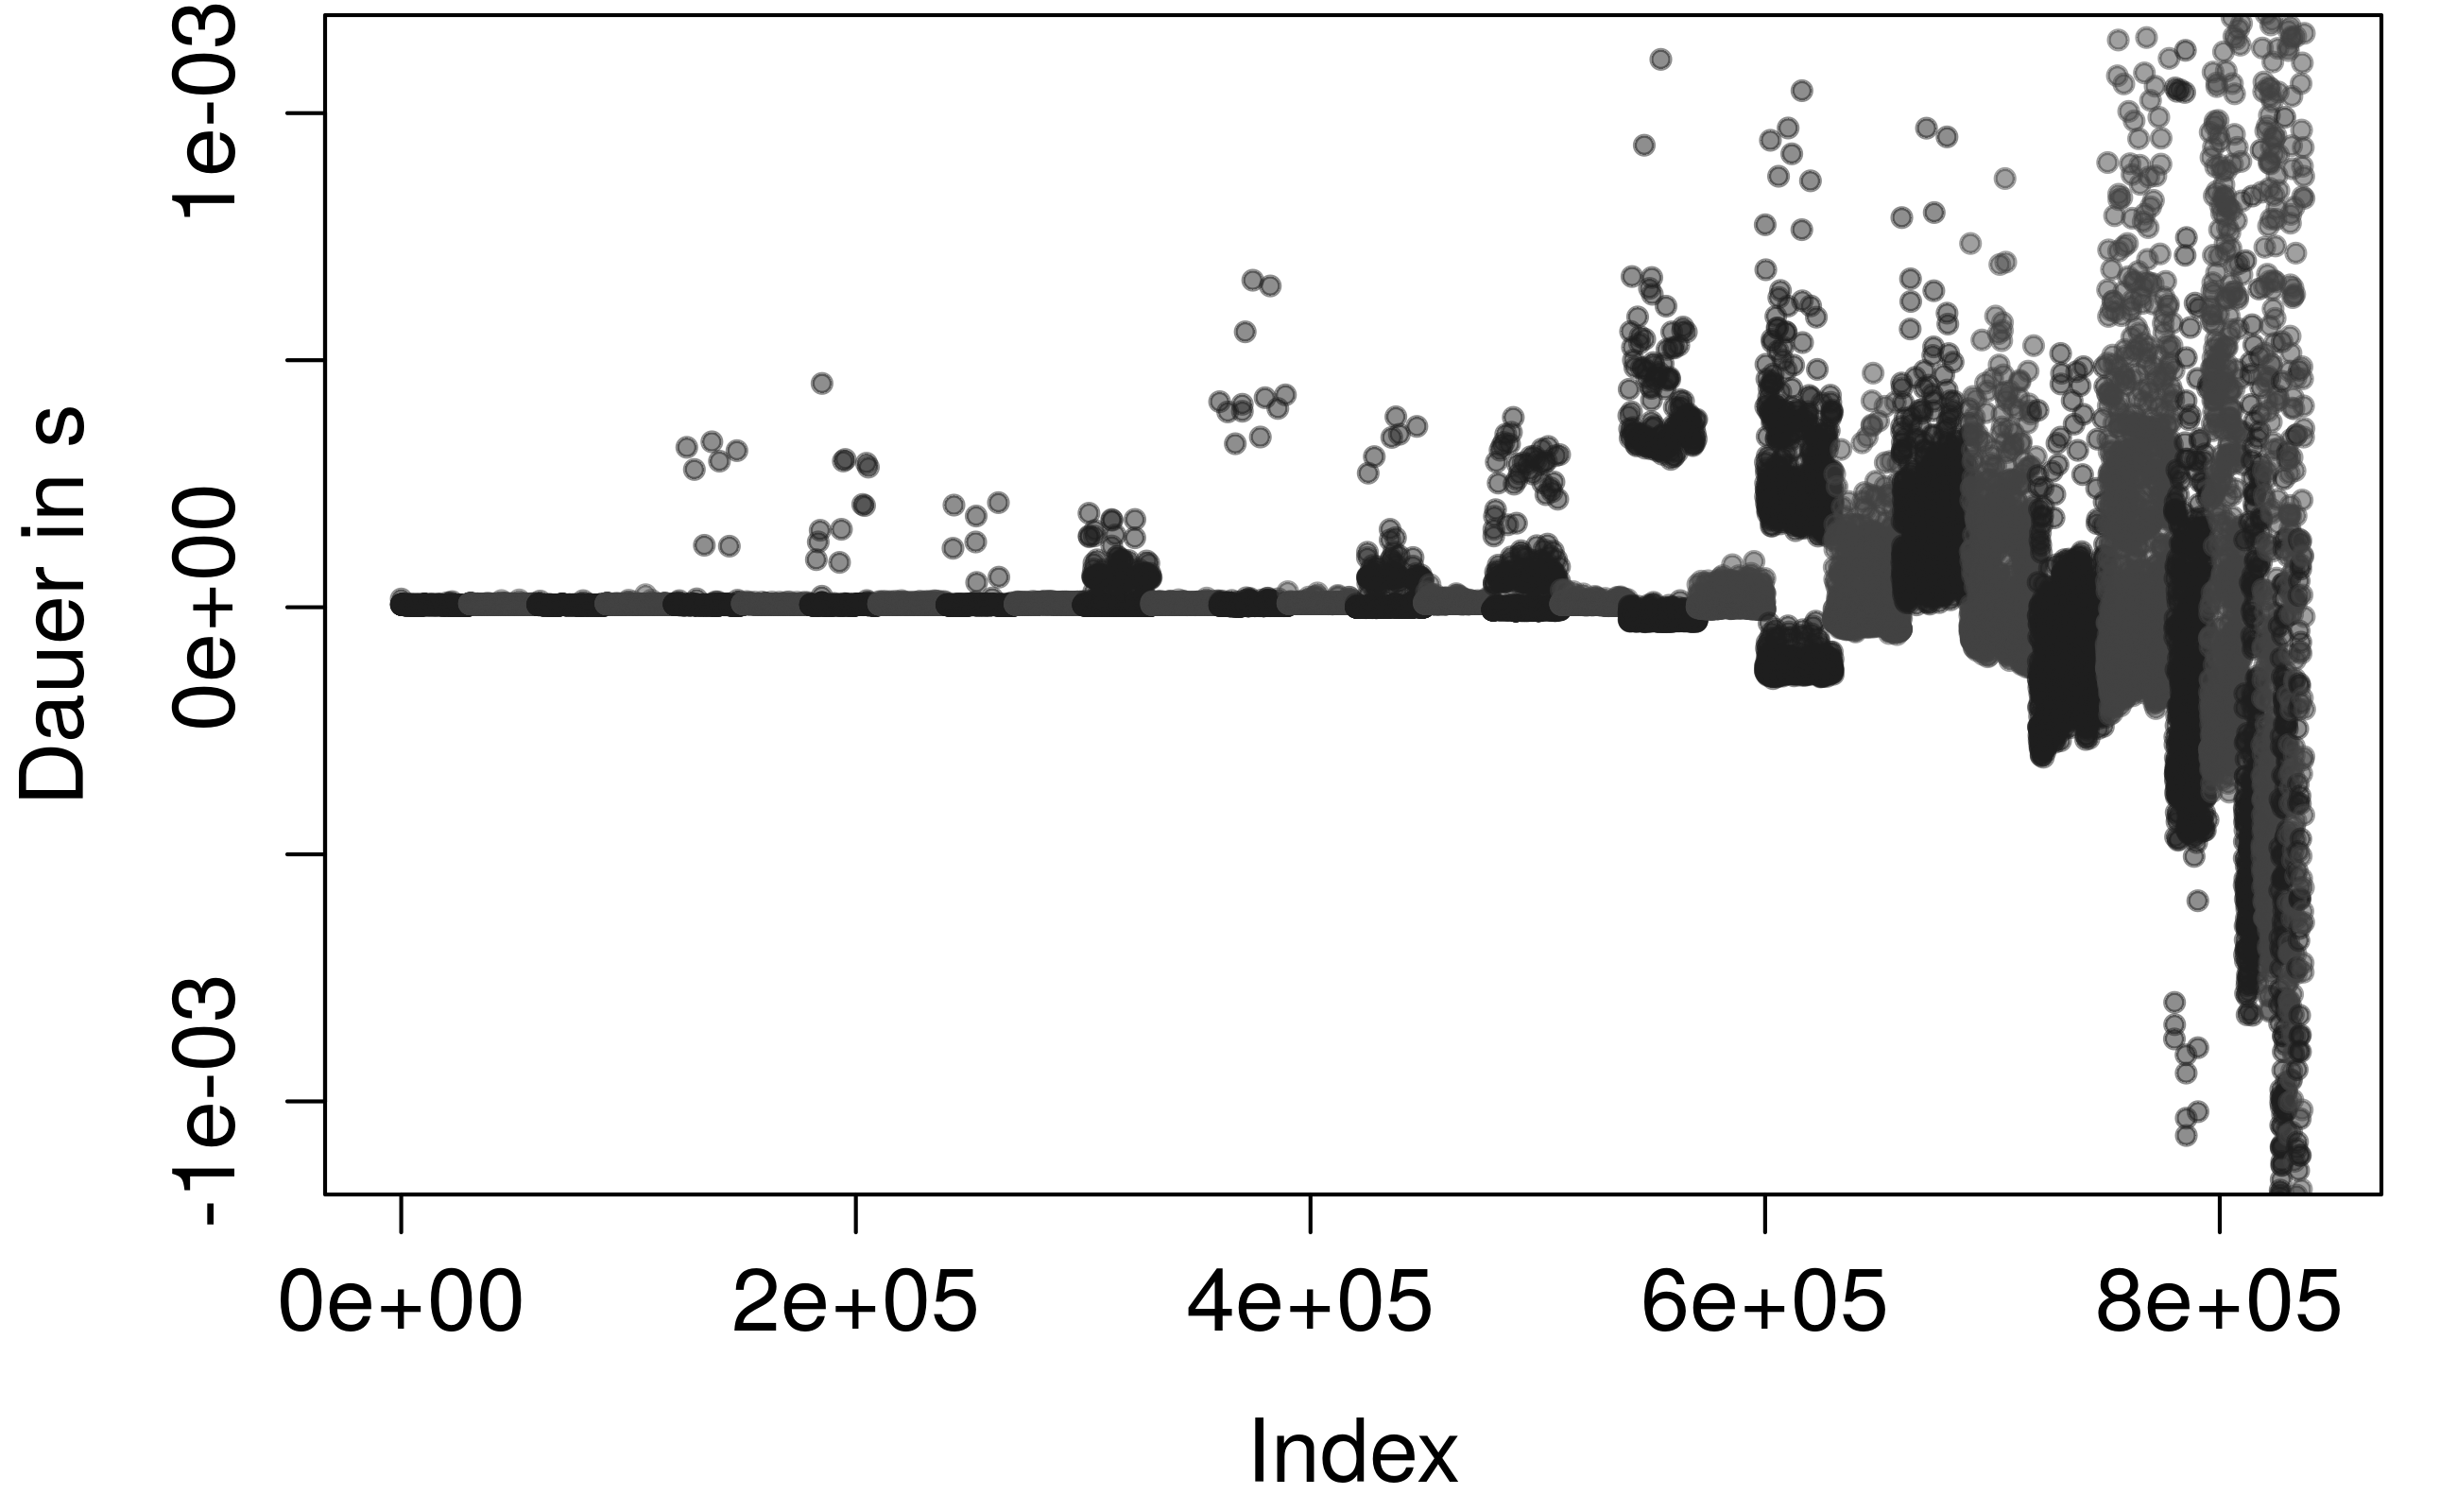
\includegraphics[width=.43\textwidth]{Bilder/Plots/error_class/exploration/linreg_error_seq_all.png}
	}
	\subfloat[Farblich markierte Fehlerklassen]{
		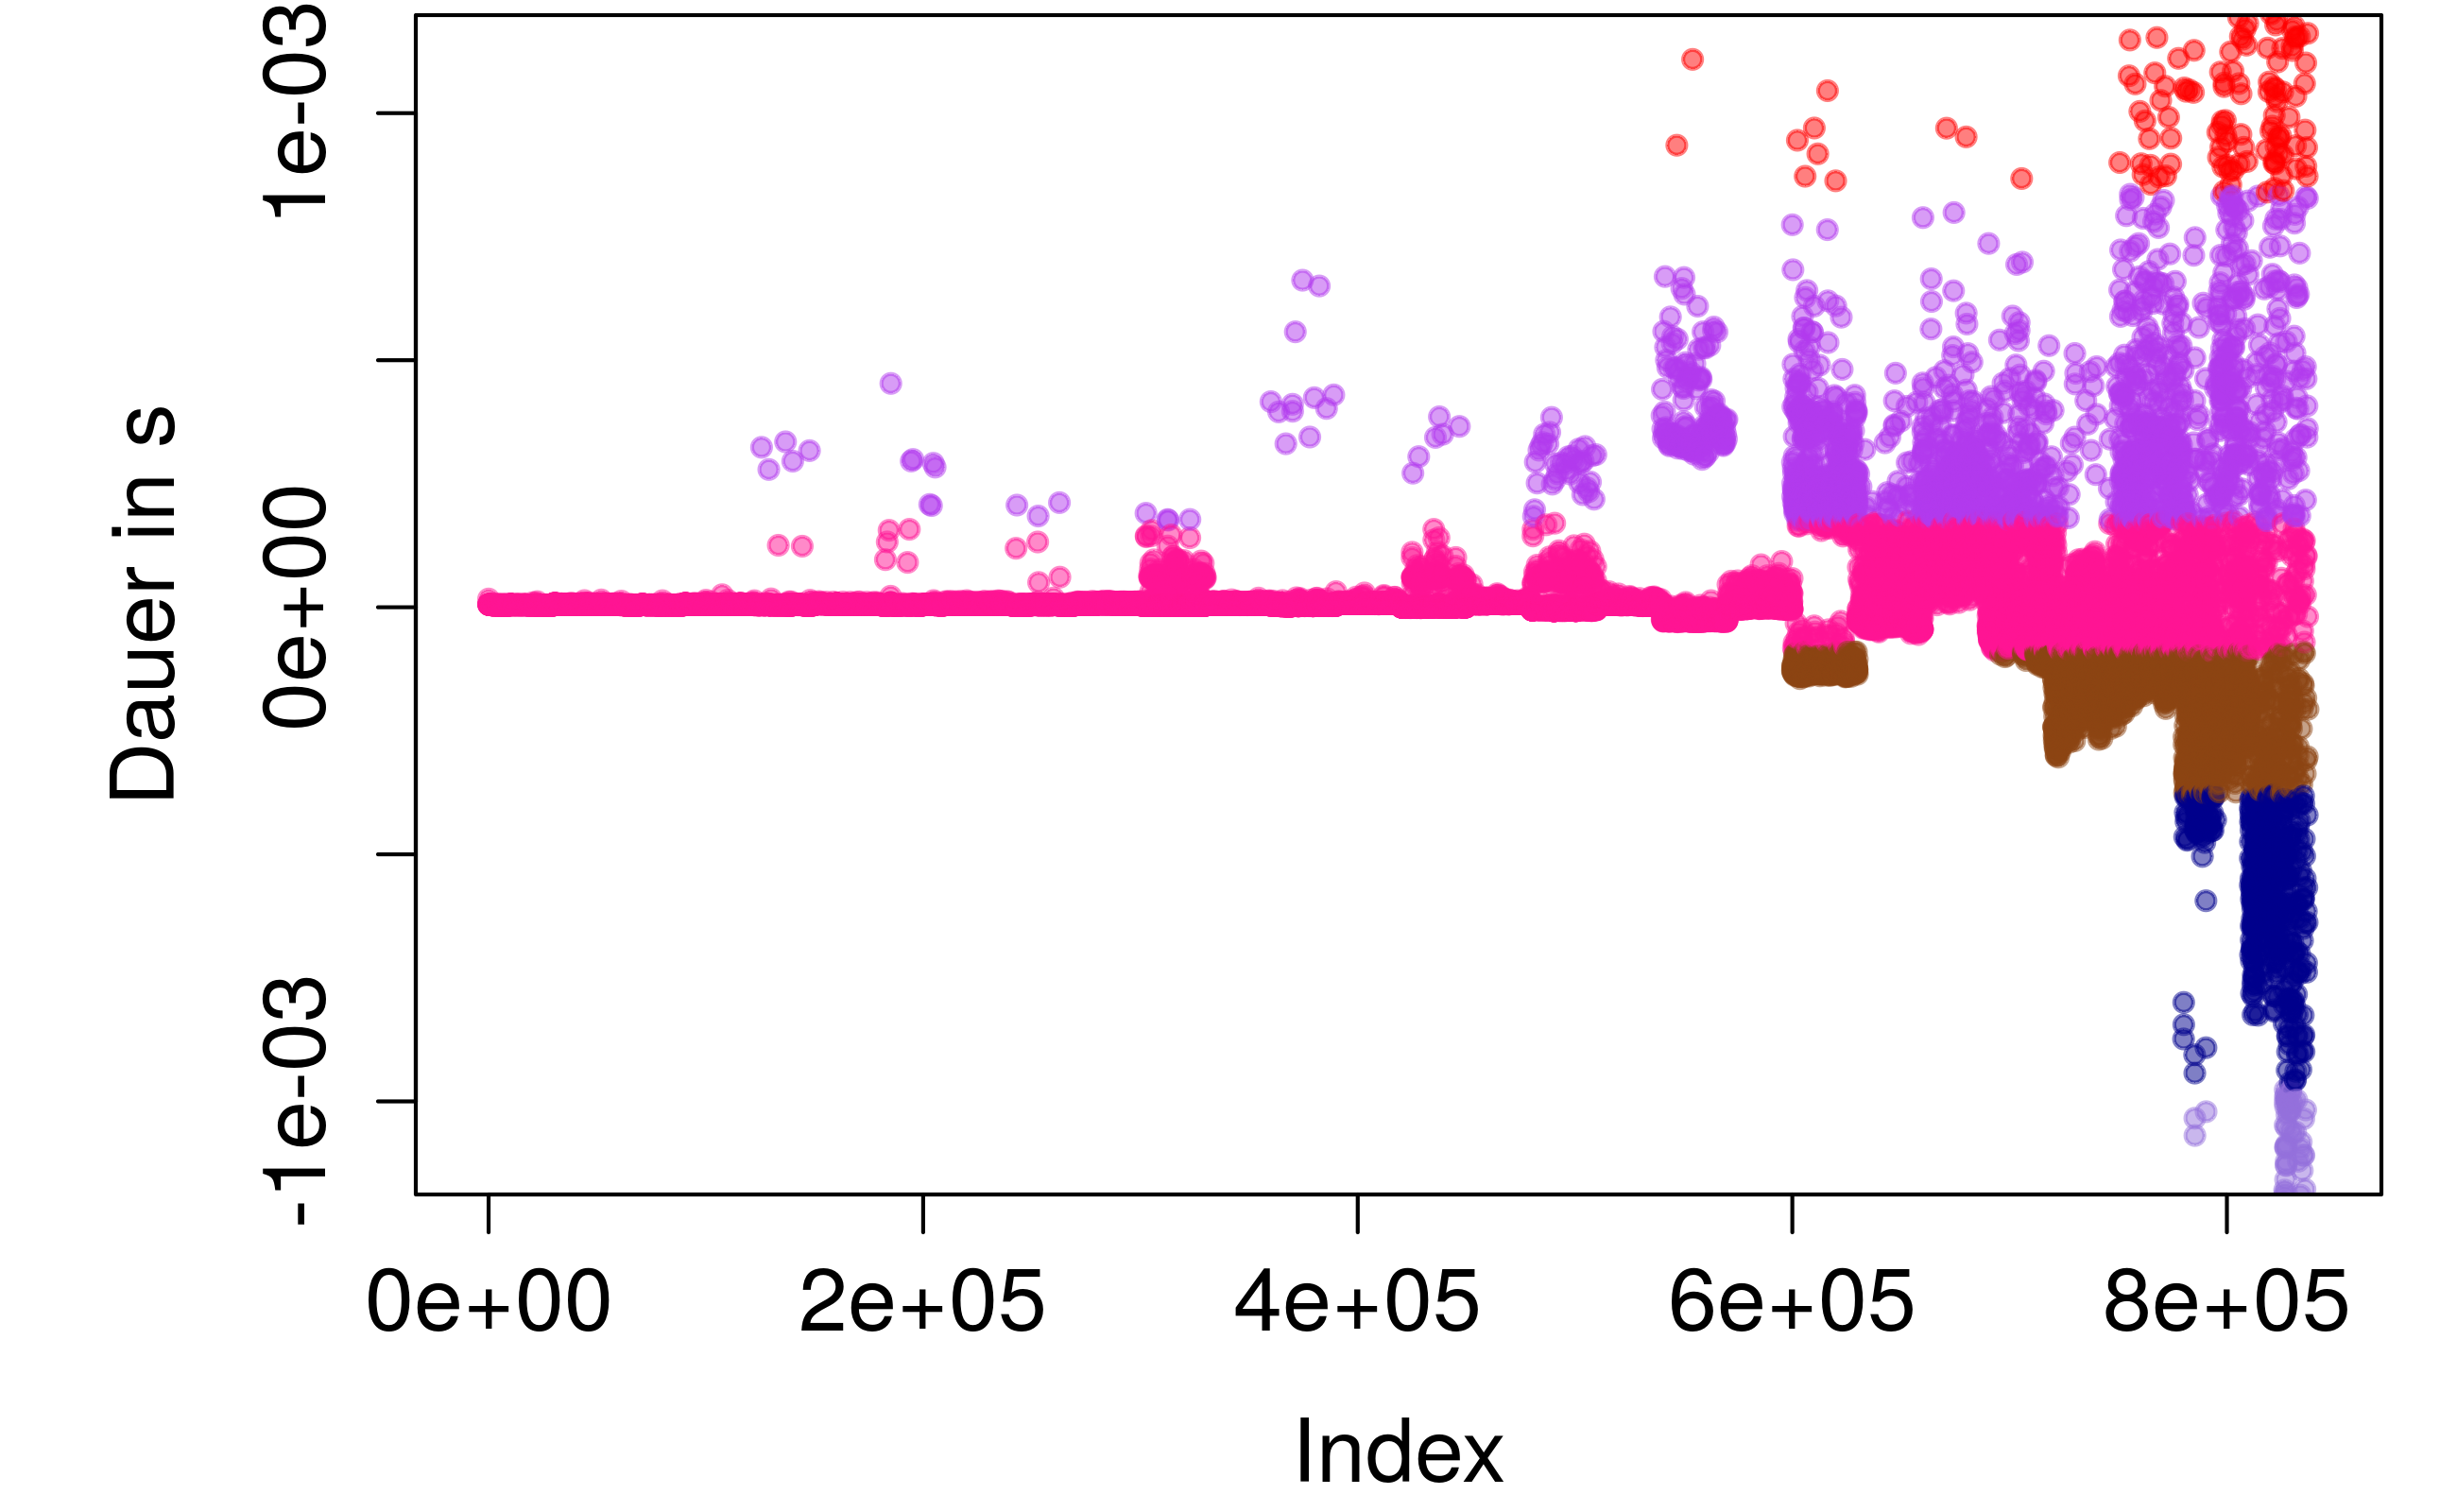
\includegraphics[width=.43\textwidth]{Bilder/Plots/error_class/exploration/linreg_error_clustering_seq_all.png}
	}\\
	\subfloat[Fehler des Modells \glqq LinReg G\grqq{} auf cached-off0-seq, in Zeitreihe, ohne die äußersten 1\%]{
		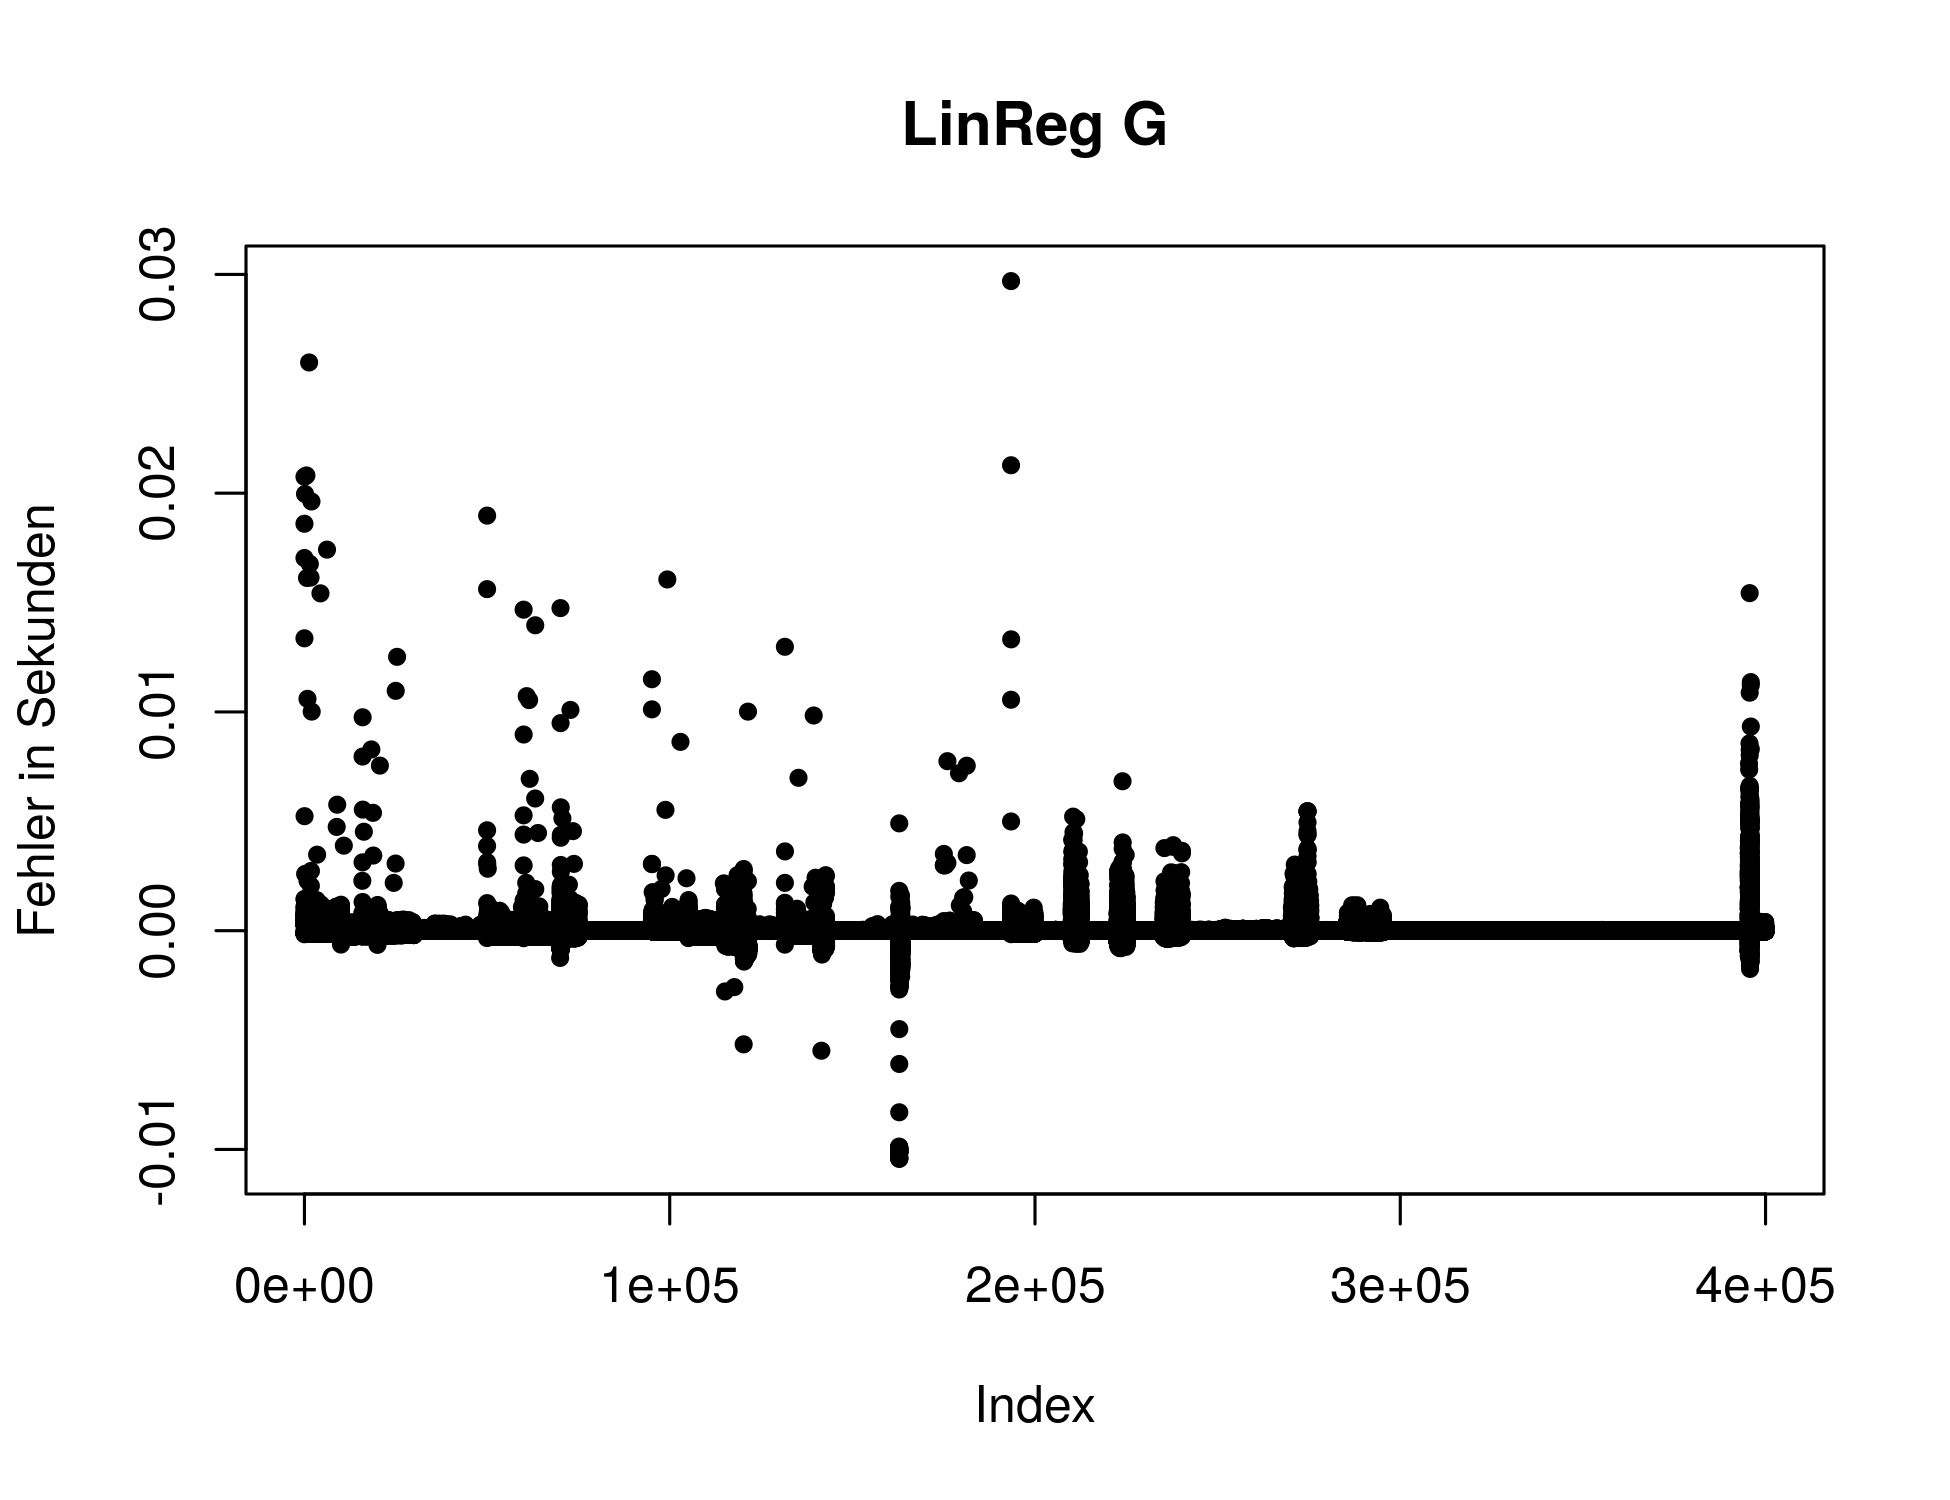
\includegraphics[width=.43\textwidth]{Bilder/Plots/error_class/exploration/linreg_error_seq.png}
	}
	\subfloat[Farblich markierte Fehlerklassen, ohne die äußersten 1\%]{
		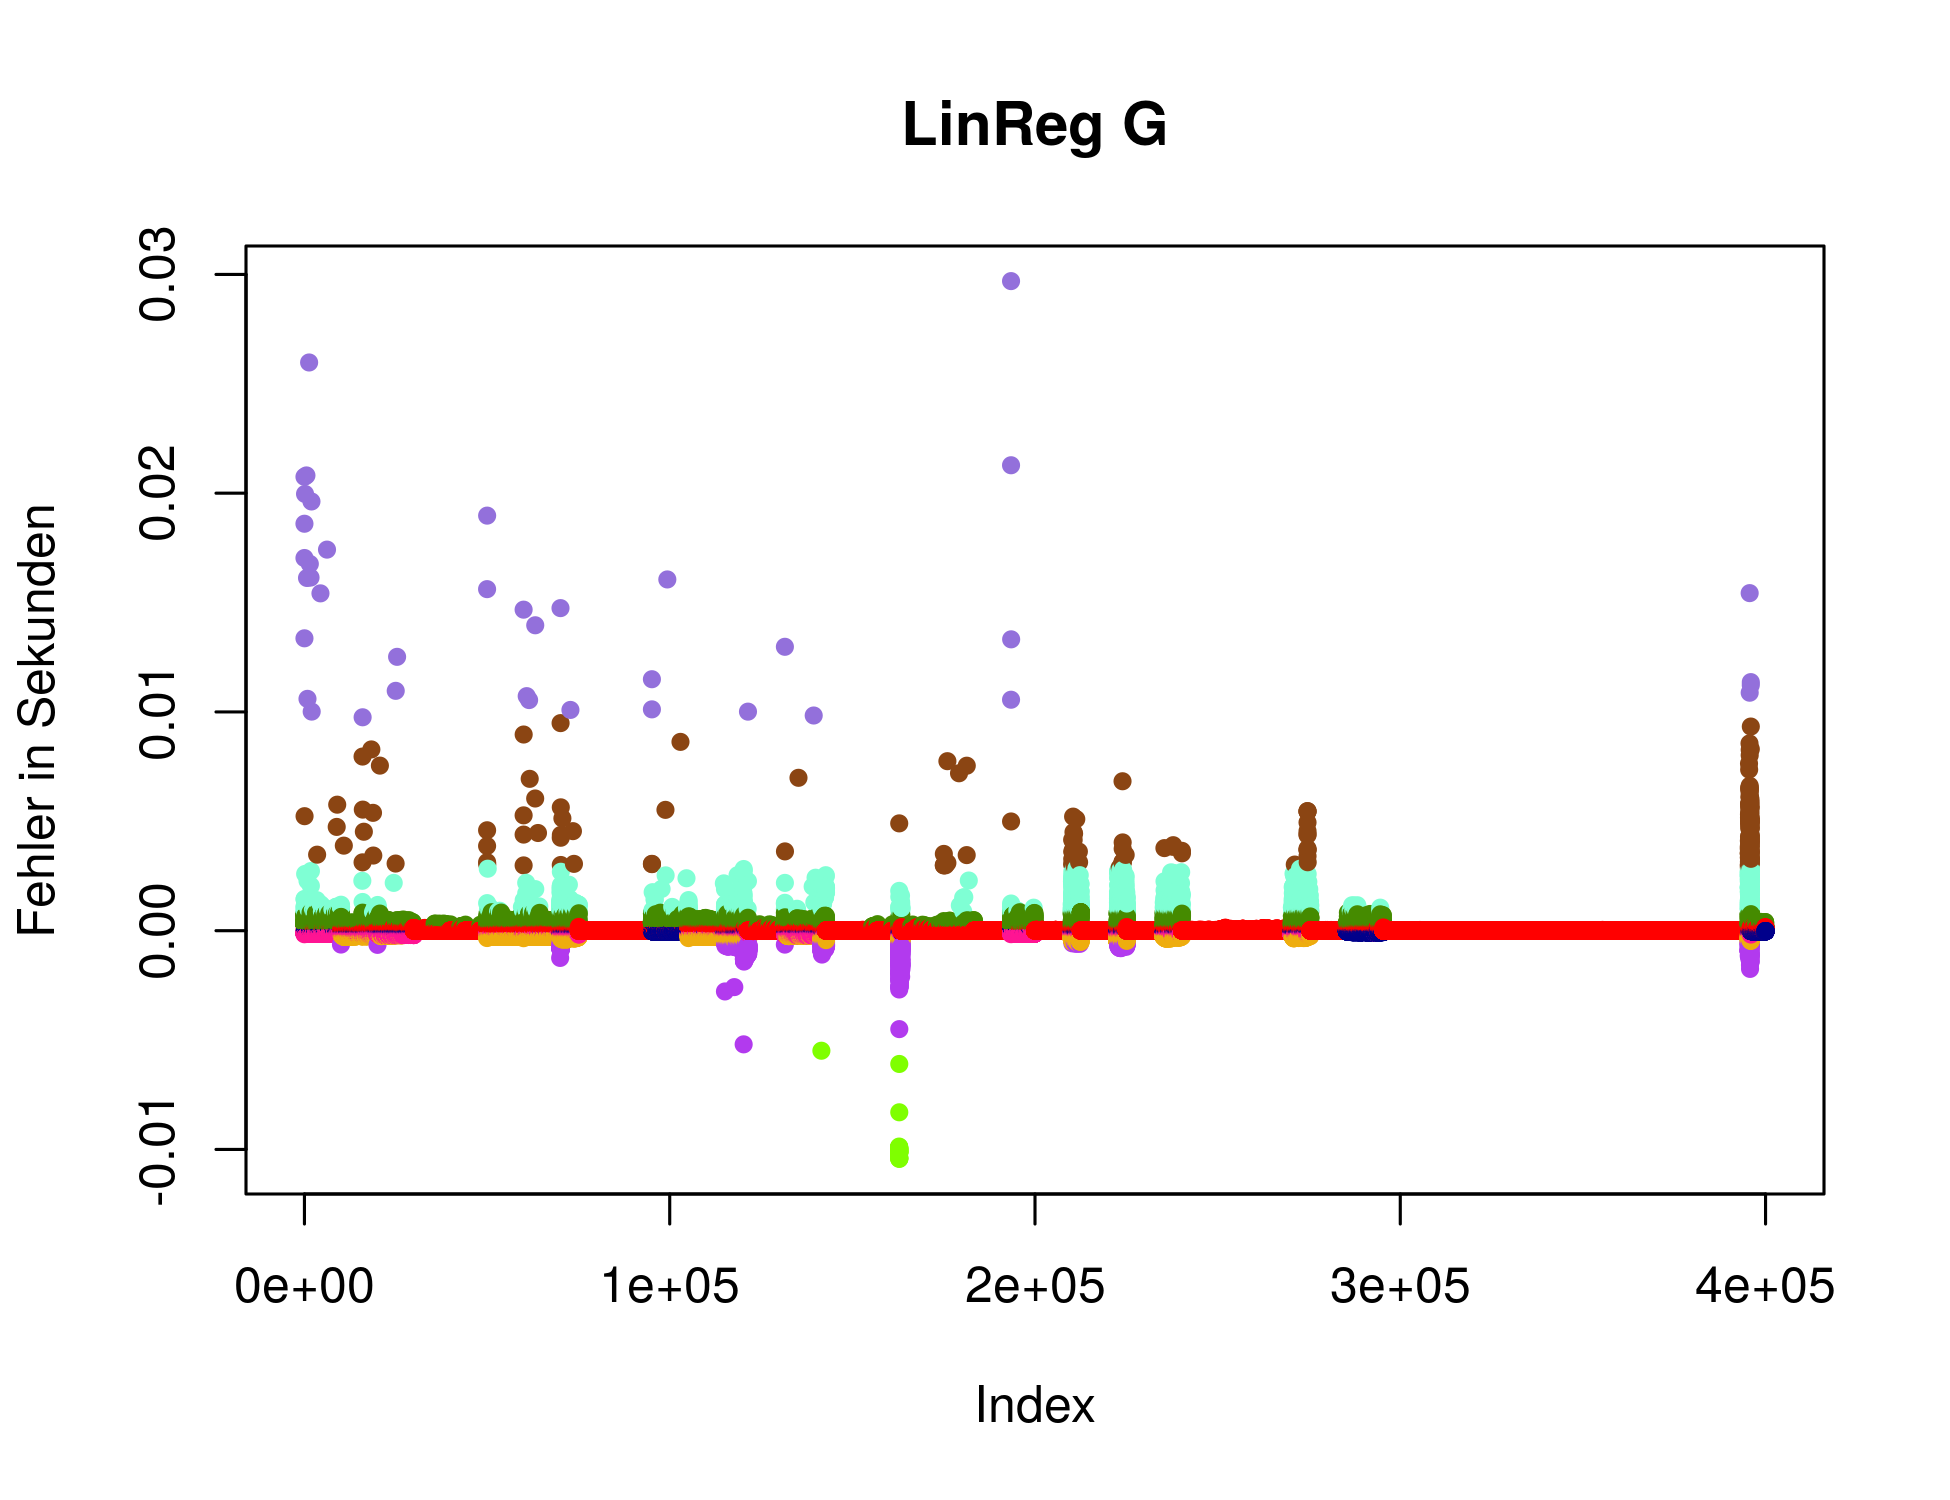
\includegraphics[width=.43\textwidth]{Bilder/Plots/error_class/exploration/linreg_error_clustering_seq.png}
	}\\
	\subfloat[Fehler des Modells \glqq LinReg G\grqq{} auf cached-off0-seq, sortiert]{
		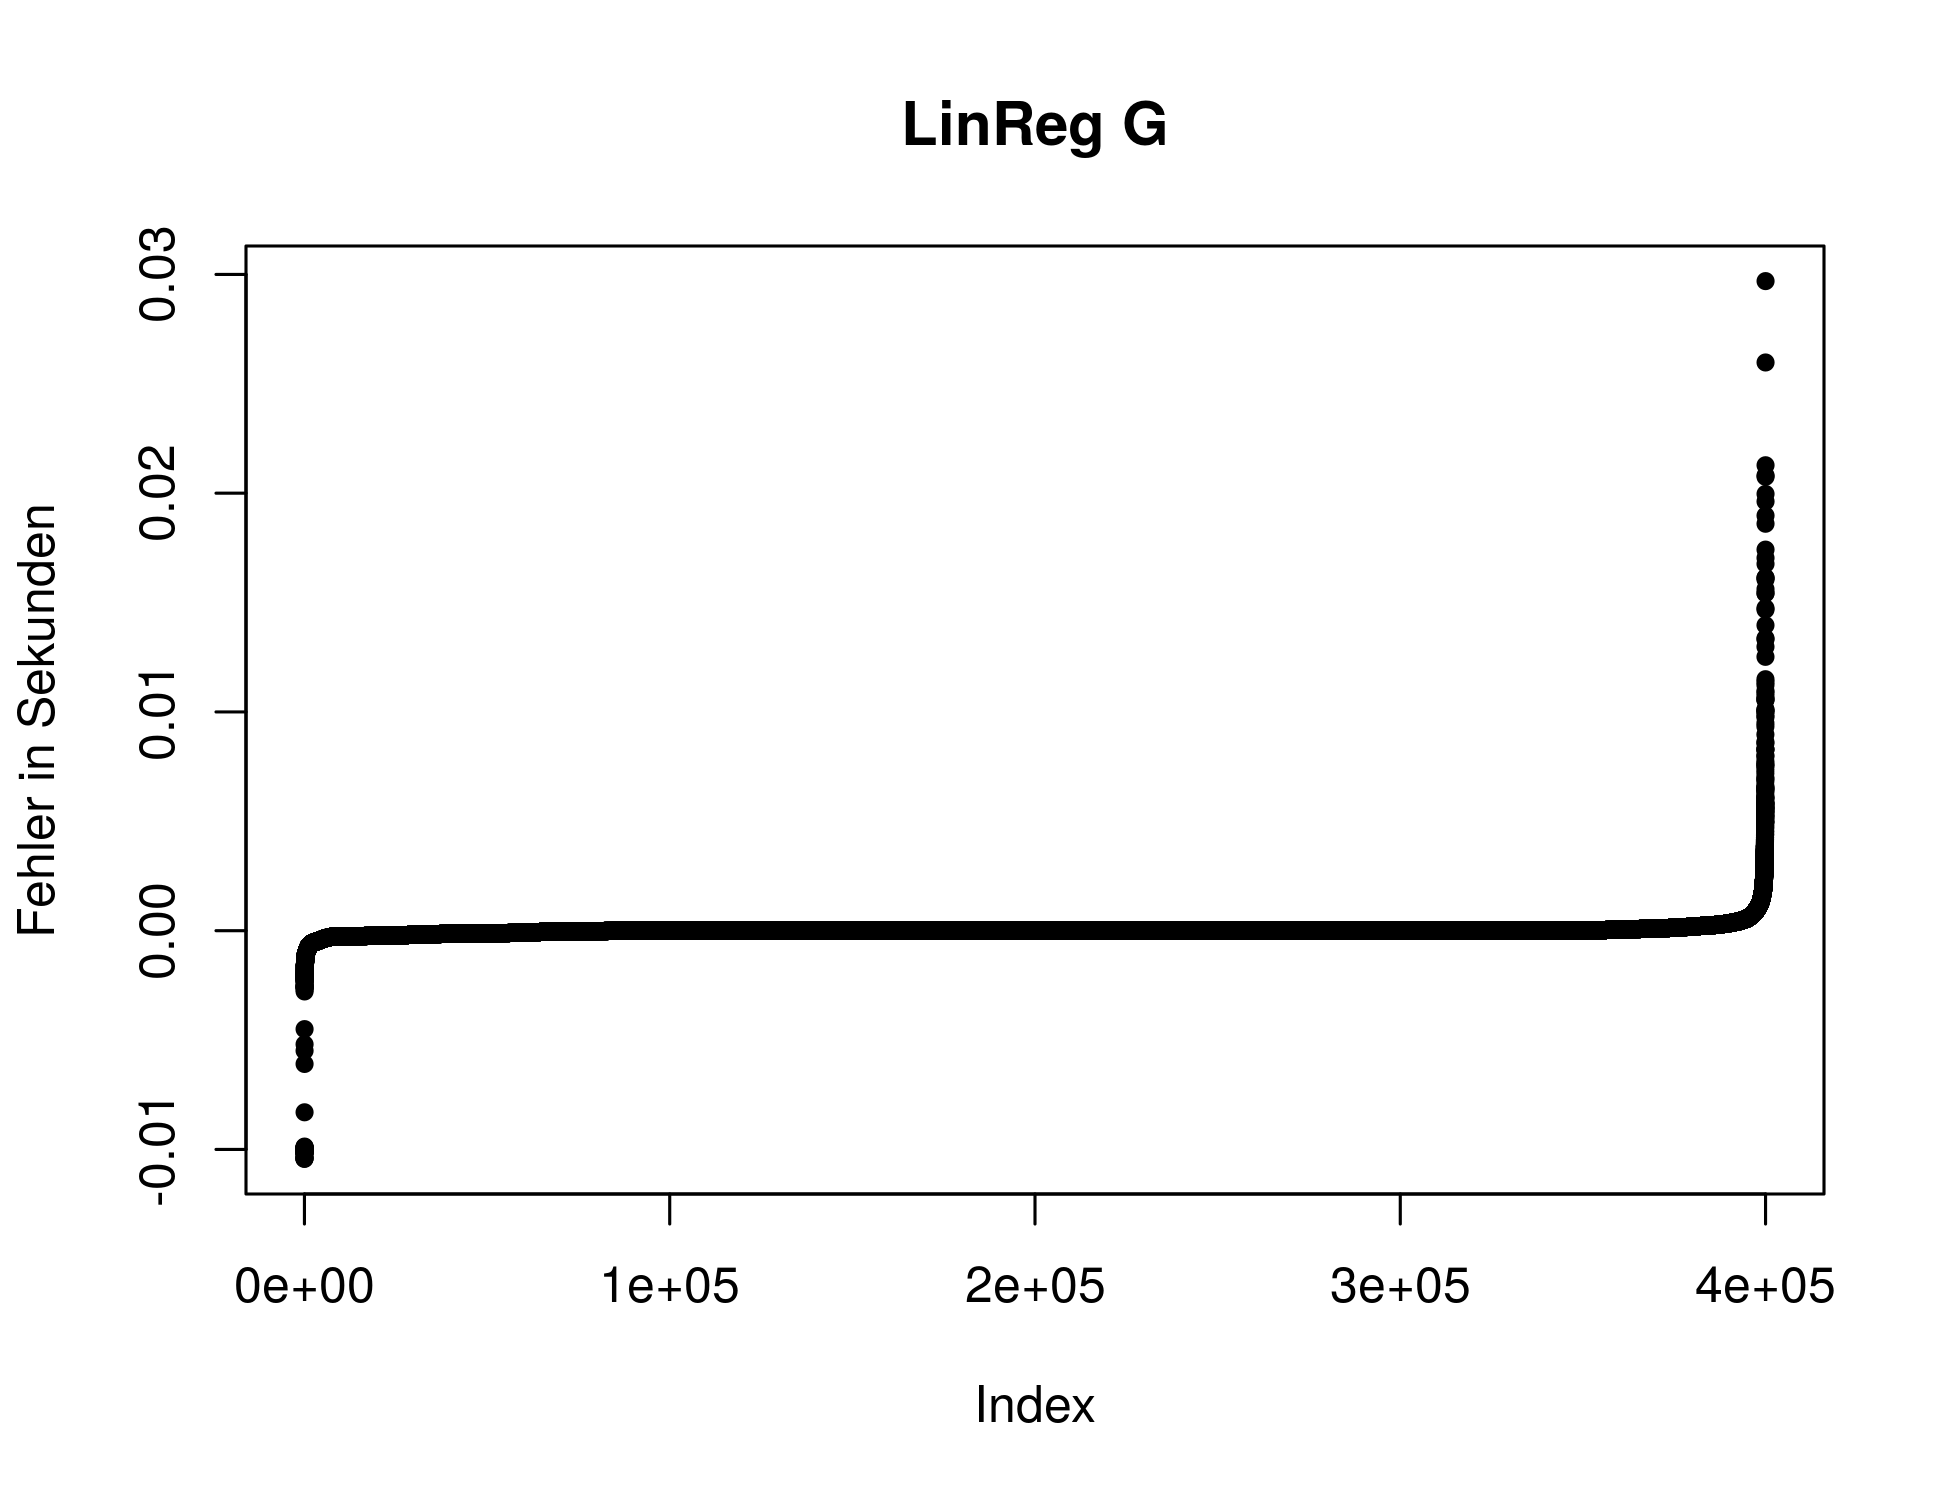
\includegraphics[width=.43\textwidth]{Bilder/Plots/error_class/exploration/linreg_error_sorted_seq.png}
	} 	
	\subfloat[Farblich markierte Fehlerklassen]{
		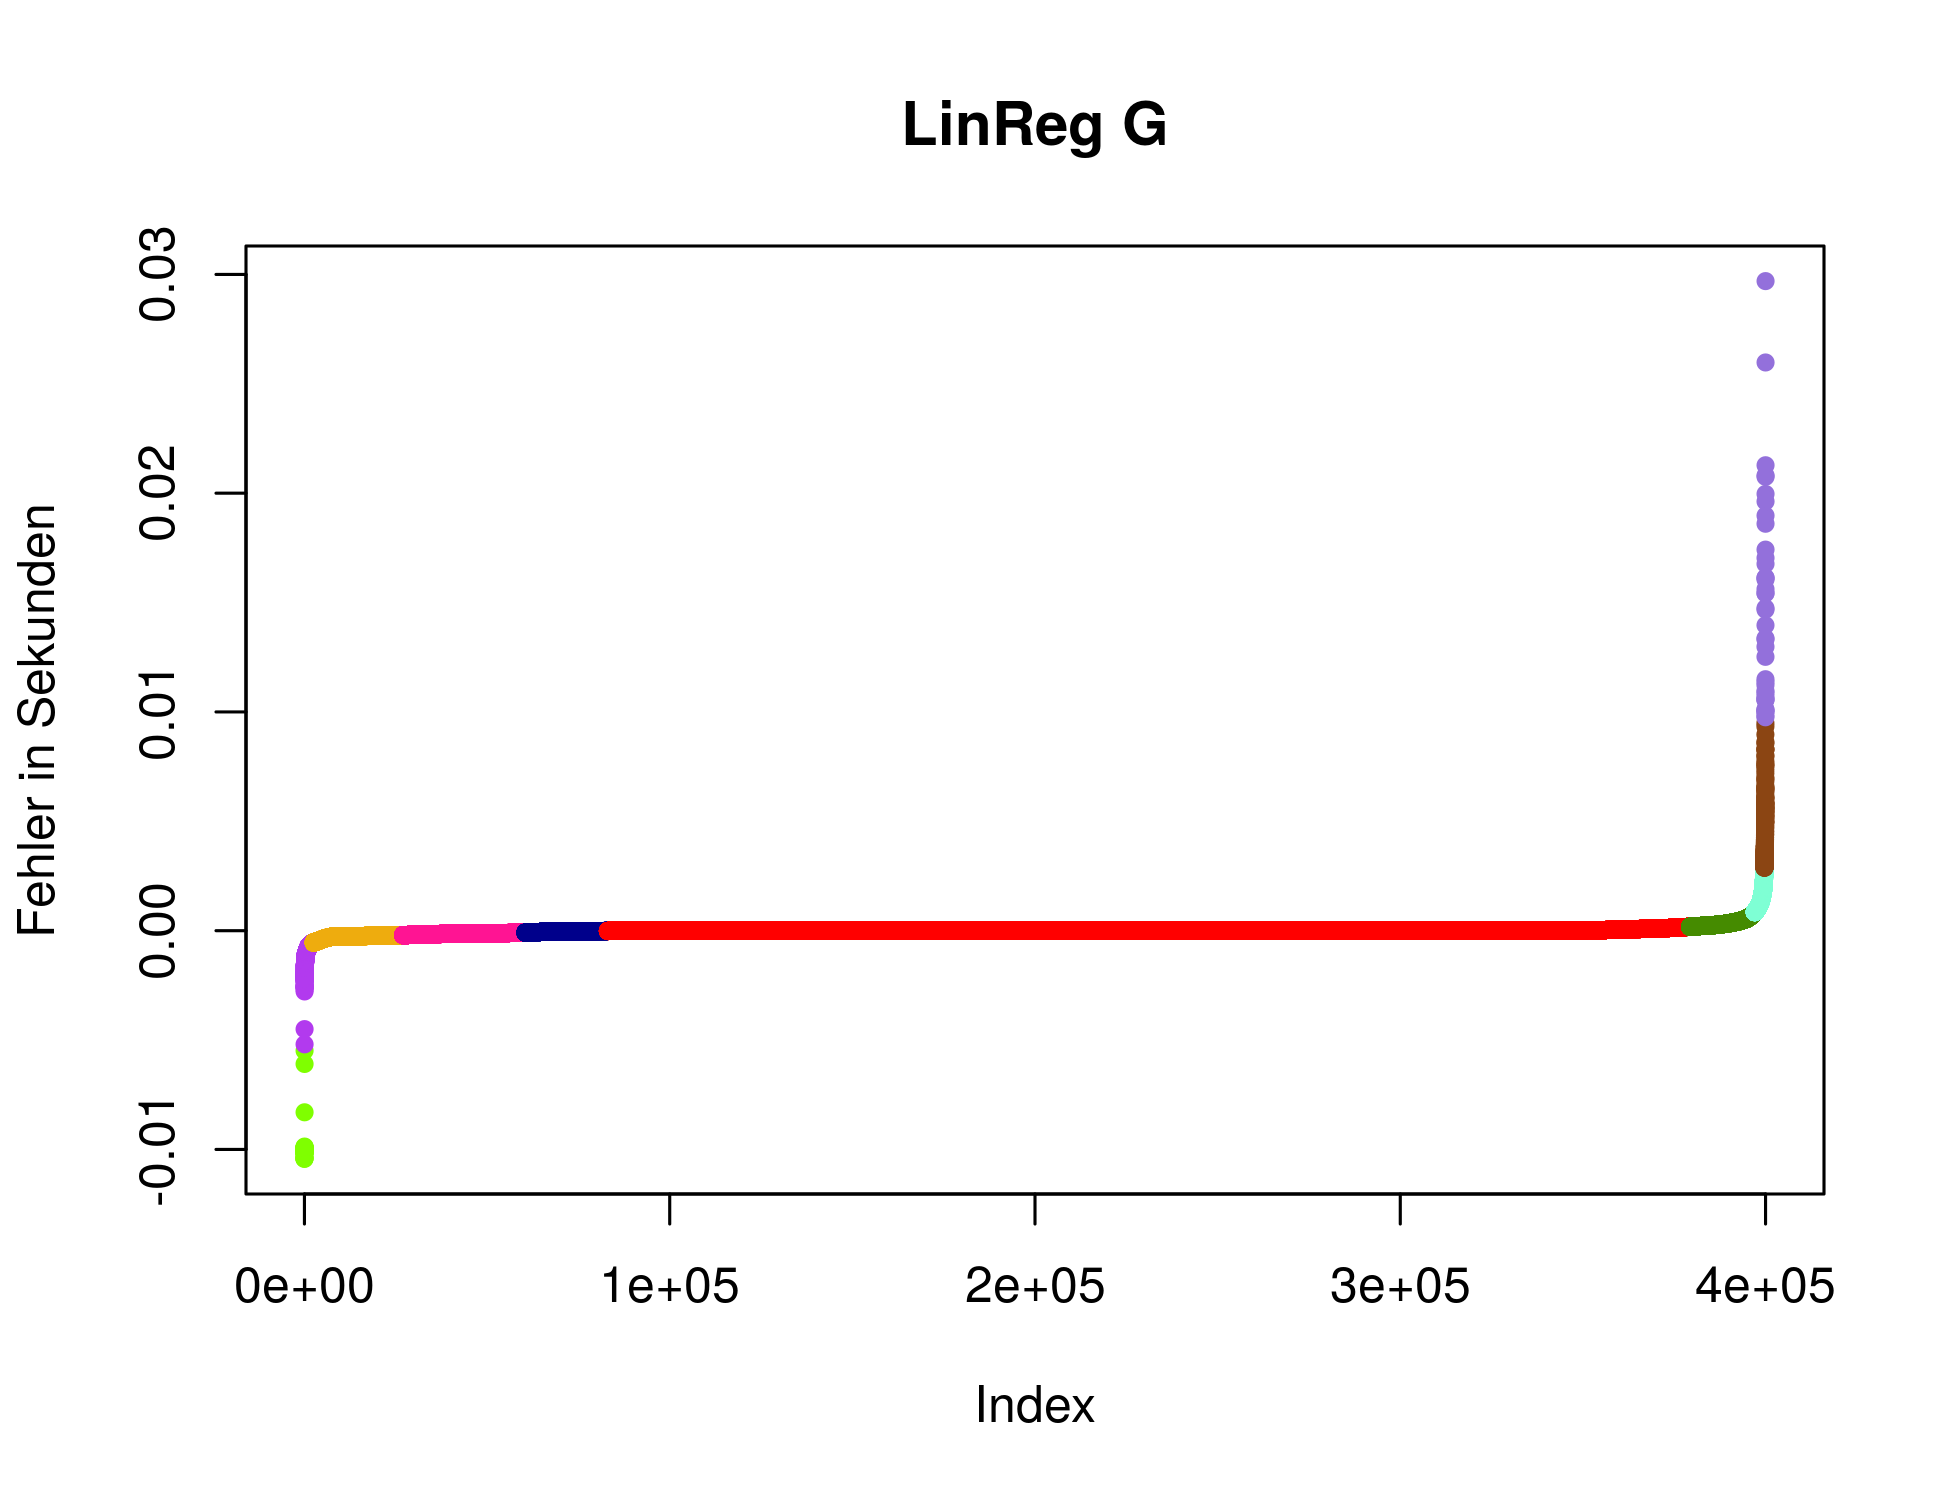
\includegraphics[width=.43\textwidth]{Bilder/Plots/error_class/exploration/linreg_error_sorted_clustering_seq.png}
	}\\	
	\caption{Verwendung des K-Means Algorithmus zur Bestimmung der Fehlerklassen auf cached-off0-rnd mit der Vorhersage von \glqq LinReg G\grqq}
	\label{fig:error_class_clustering_seq}
\end{figure} 

\begin{figure}
	\centering
	\subfloat[Fehler des Modells \glqq LinReg G\grqq{} auf cached-off0-rnd, in Zeitreihe]{
		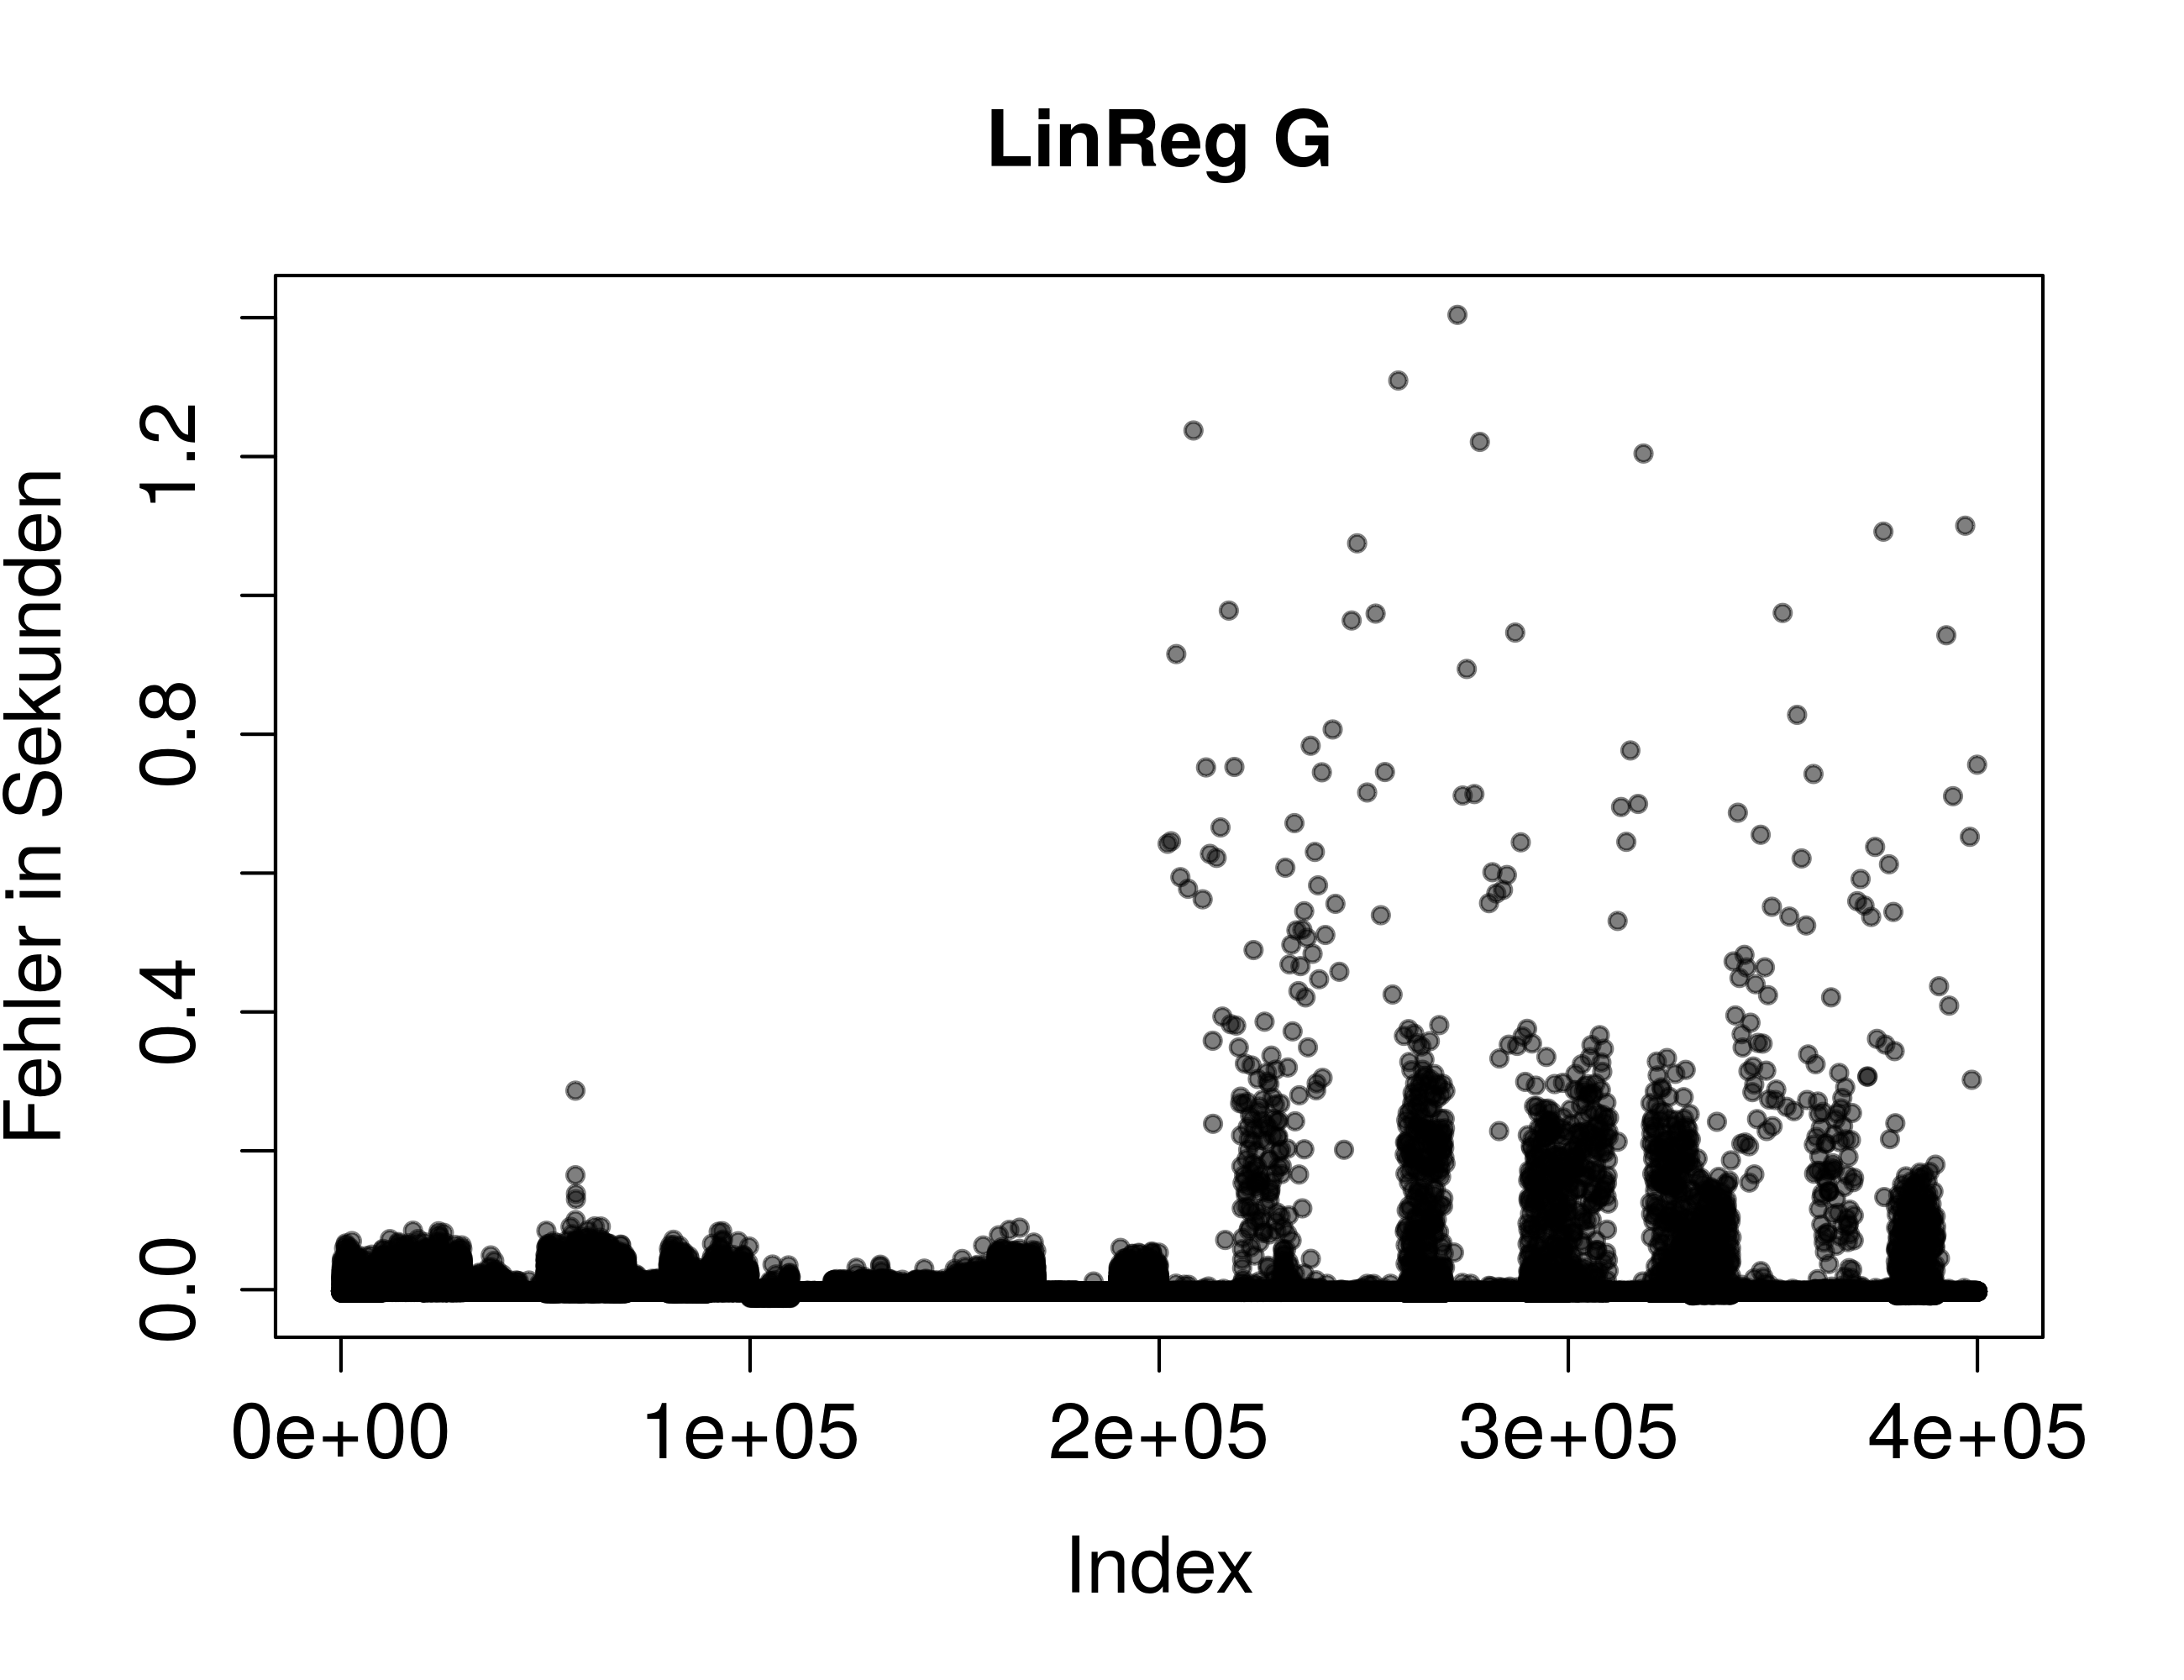
\includegraphics[width=.43\textwidth]{Bilder/Plots/error_class/exploration/linreg_error_rnd_all.png}
	}
	\subfloat[Farblich markierte Fehlerklassen]{
		\includegraphics[width=.43\textwidth]{Bilder/Plots/error_class/exploration/linreg_error_clustering_rnd_all.png}
	}\\
	\subfloat[Fehler des Modells \glqq LinReg G\grqq{} auf cached-off0-rnd, in Zeitreihe, ohne die äußersten 1\%]{
		\includegraphics[width=.43\textwidth]{Bilder/Plots/error_class/exploration/linreg_error_rnd.png}
	} 	
	\subfloat[Farblich markierte Fehlerklassen, ohne die äußersten 1\%]{
		\includegraphics[width=.43\textwidth]{Bilder/Plots/error_class/exploration/linreg_error_clustering_rnd.png}
	}\\
	\subfloat[Fehler des Modells \glqq LinReg G\grqq{} auf cached-off0-rnd, sortiert]{
		\includegraphics[width=.43\textwidth]{Bilder/Plots/error_class/exploration/linreg_error_sorted_rnd.png}
	} 	
	\subfloat[Farblich markierte Fehlerklassen]{
		\includegraphics[width=.43\textwidth]{Bilder/Plots/error_class/exploration/linreg_error_sorted_clustering_rnd.png}
	}\\
	\caption{Verwendung des K-Means Algorithmus zur Bestimmung der Fehlerklassen auf cached-off0-rnd mit der Vorhersage von \glqq LinReg G\grqq}
	\label{fig:error_class_clustering_rnd}
\end{figure} 

Anhand einer weiteren Betrachtung der Fehlerklassen sollen die Unterschiede zwischen den Klassen auf den beiden Datensätzen analysiert werden.
In Abbildung \ref{fig:error_classes_switched} sind die Punkte den Klassen aus dem jeweils anderen Datensatz zugeordnet worden. Die Neuzuordnung wurde ebenso durchgeführt, wie es der K-Means Algorithmus bei der Erstzuordnung gemacht hat. Für alle Klassen wurde der mittlere Fehlerwert nach Zuordnung der Punkte auf dem ursprünglichen Datensatz berechnet und dann wurde jeder Datenpunkt im anderen Datensatz der Klasse mit dem Mittelwert zugeordnet, der am nächsten an seinem eigenen Fehlerwert liegt.\\ 
Für cached-off0-seq ist deutlich zu sehen (\ref{fig:error_classes_switched} c) ), dass 99\% der Punkte der selben Fehlerklasse zugeordnet worden. Dagegen wird bei cached-off-rnd in dem Bereich mit kleinerem Fehler nun stärker als zuvor (\ref{fig:error_class_clustering_rnd} d) ) differenziert, während alle größeren Fehler die selbe Klasse haben.

\begin{figure}
	\centering
	\subfloat[Klassen aus cached-off0-rnd auf cached-off0-seq]{
		\includegraphics[width=.43\textwidth]{Bilder/Plots/error_class/exploration/rnd_linreg_classes_on_seq_all.png}
	}
	\subfloat[Klassen aus cached-off0-seq auf cached-off0-rnd]{
		\includegraphics[width=.43\textwidth]{Bilder/Plots/error_class/exploration/seq_linreg_classes_on_rnd_all.png}
	}\\
	\subfloat[Klassen aus cached-off0-rnd auf cached-off0-seq, ohne die äußersten 1\%]{
		\includegraphics[width=.43\textwidth]{Bilder/Plots/error_class/exploration/rnd_linreg_classes_on_seq.png}
	}
	\subfloat[Klassen aus cached-off0-seq auf cached-off0-rnd, ohne die äußersten 1\%]{
		\includegraphics[width=.43\textwidth]{Bilder/Plots/error_class/exploration/seq_linreg_classes_on_rnd.png}
	}
	\caption{Farblich markierte Fehlerklassen, unter Verwendung der Fehlerklassen, die aus aus dem jeweils anderen Datensatz stammen}
	\label{fig:error_classes_switched}
\end{figure} 

In \ref{tab:error_classes_switched} wurden die Fehlerklassen nun nach mittleren Durchsatz sortiert. (\textbf{WARUM?}) \textbf{BESCHREIBUNG DER TABLLE}
In der Tabelle ist ablesbar, was ich zuvor bereits anhand des Graphen gedeutet habe, für cached-off0-seq befinden sich mit vertauschten Fehlerklassen 399709 von 400000 Punkten in der selben Klasse. Dies ist die Klasse, die den geringsten Durchsatz hat und in der LinReg G zuvor auf dem randomisierten Datensatz den größten Fehler gemacht hat.
Die Fehlerklassen von cached-off0-seq sind dagegen sogar recht gut zur Differenzierung der Datenpunkte auf cached-off0-rnd nutzbar, wie in Tabelle \ref{tab:error_classes_switched} b) an den Werten für \glqq Anzahl auf rnd \grqq{} zu entnehmen ist. Dies ist dem Umstand geschuldet, dass die Fehlerklassen von cached-off0-seq in dem Bereich mit kleinem Fehler stark differenziert und die meisten Punkte sich auch auf cached-off0-rnd dort befinden.
Für eine bessere Vorhersage der Messdaten würden sich diese Klassen auf beiden Datensätzen nicht eignen. Auf cached-off0-seq, da sich praktisch alle Punkte in der selben Klasse befinden und auf cached-off0-rnd, weil in den entscheidenden schlechteren Vorhersagen von LinReg G keine Unterscheidung stattfindet.

\begin{table}
	\scriptsize
	\subfloat[Fehlerklassen von cached-off0-seq]{
		\begin{tabular}{|r|r|r|r|r|r|r|}\hline%
			Klasse & mittlerer Durchsatz (B/s) & Min (s) & Durchschnitt (s) & Max (s) & Zugeordnet auf seq & Zugeordnet auf rnd \\\hline\hline
			\csvreader[late after line=\\\hline]%
			{CSV/error_class/seq_linreg_classes_on_rnd.csv}{tp=\tp,idx = \idx,rndcount=\rndcount,minerror=\minerror, meanerror = \meanerror, maxerror = \maxerror, seqcount = \seqcount}%
			{\idx & \tp & \minerror & \meanerror & \maxerror & \seqcount & \rndcount}%
		\end{tabular}
	}\\
	\subfloat[Fehlerklassen von cached-off0-rnd]{
		\begin{tabular}{|r|r|r|r|r|r|r|}\hline%
			Klasse & mittlerer Durchsatz (B/s) & Min (s) & Durchschnitt (s) & Max (s) & Zugeordnet auf rnd & Zugeordnet auf seq \\\hline\hline
			\csvreader[late after line=\\\hline]%
			{CSV/error_class/rnd_linreg_classes_on_seq.csv}{tp=\tp,idx = \idx, rndcount=\rndcount,minerror=\minerror, meanerror = \meanerror, maxerror = \maxerror, seqcount = \seqcount}%
			{\idx & \tp & \minerror & \meanerror & \maxerror & \rndcount & \seqcount}%
		\end{tabular}
	}
	
	\caption{Fehlerklassen sortiert von kleinem zu großem Zentrum des Clusters (Durchschnittlicher Fehler). Einmal die Anzahl Punkte, die den Klassen auf dem Datensatz zugeordnet wurden, von dem sie auch stammen. Zudem die Anzahl Punkte, die den Klassen auf dem anderen Datensatz zugeordnet werden würden.}
	\label{tab:error_classes_switched}
\end{table}

\section{Leistungsvorhersage}
Zu jedem Modell schreiben, welche Attribute und Parameter sich als geeignet herausgestellt haben. Ergebnisse anhand von Graphen veranschaulichen.\\
Ergebnisse für verschiedene Fälle vergleichen, seq,rnd\\
Ergebnisse von bagging

\subsection{Analyse der trivialen Modelle}

Die Ergebnisse der in \textbf{ABSCHNITT} beschriebenen trivialen Modelle sind in \ref{tab:triv} zu sehen. Eine positive Beobachtung in den Ergebnissen auf cached-off0-seq ist zunächst, dass alle Metriken einen ähnlichen Trend der  Modelle aufzeichnen. Das gilt im Wesentlichen auch für cached-off0-rnd, jedoch hat das Modell "Median agg" einen sehr hohen maximalen Fehler. Dies führt entsprechend zu einem vergleichsweise hohen RMQA-Wert, obwohl der relative arithmetische Fehler noch recht gering ist. \\
Wie erwartet (\textbf{ABSCHNITT}) sind die Vorhersagen auf dem randomisierten Datensatz schwieriger zu machen, sodass die Fehlerwerte höher sind. Dies gilt insbesondere für die Modelle, die auf linearer Regression basieren, hier sind die Werte $30-140$ mal höher. Eine Ausnahme ist "Median agg LinReg-Fehlerklasse", das Modell kann eine weiterhin sehr gute mittlere Vorhersage treffen, nur die Ausreißer nach oben scheinen zugenommen zu haben, sodass RMax und RMQA höher als bei sequentiellen Datensatz sind.\\
Allgemein sind die Ergebnisse bereits überraschend gut. Ein durchschnittlicher Fehler von $5\%$ auf cached-off0-seq bzw. $7-12\%$ auf cached-off0-rnd durch die Modelle, die Fehlerklassen ausnutzen, deutet daraufhin, dass die Vorgänge im E/A-System im Wesentlichen korrekt repräsentiert werden. Ob über eine größere Messreihe ein geringerer durchschnittlicher Fehler als $5\%$ überhaupt erreicht werden kann, ist fraglich, da das Messrauschen durch unvorhersehbare Ereignisse sowohl auf System-, als auch Bauteilebene, in diesen Bereichen eine zu große Bedeutung zukommt.\\
Die Modelle mit linearer Regression führen auf cached-off0-seq auch bereits zu zufriedenstellenden Ergebnissen, während sie auf cached-off0-rnd kaum sinnvolle Vorhersagen machen zu scheinen. Die Modelle lassen sich für die Datensätze jeweils in drei Gruppen (gut, mittel, schlecht) unterteilen. Auf beiden Datensätzen führen die beiden Modelle mit Fehlerklasse zu einer guten Vorhersage. "Median agg" hat jeweils eine mittel gute Leistung, während "Durchschnitt" jeweils schlecht ist. Interssant ist, dass Modelle mit linearer Regression auf dem sequentiellen Datensatz eine zufriedenstellende mittlel gute Vorhersage macht, während die Vorhersage auf dem randomisierten Messungen kaum besser als des Durschnitts-Modell ist. \\ 
Das Modell, das immer die Durchschnittsdauer vorhersagt ist als absolute untere Grenze für angewendete Modelle zu verstehen, da hier praktisch keine Expertise über die Daten eingeht. 
Tatsächlich erreicht dieses Modell die schlechtesten Ergebnisse in beiden Testfällen. Die Ansätze der rechenintensiven halten diesem Anspruch also stand und sind somit gerechtfertigt. \\
Aufgrund des geringen Nutzen der Attribute Abstand und OpTyp für die lineare Regression wird im Folgenden nur das Modell über die Zugriffsgröße betrachtet.\\

\begin{table}
	\scriptsize
	\subfloat[cached-off0-seq]{
		\begin{tabular}{|r|r|r|r|r|r|r|}\hline%
			Modell & MAF (s)  & RMAF (\%) & RMQA (\%) & RQ3 (\%) & RMax (\%) & Typ \\\hline\hline
			\csvreader[late after line=\\\hline]%
			{CSV/baselines/latex_baseline_seq_results.csv}{Modell=\Model,MAF=\MAF,RMAF=\RMAF, RMQA = \RMQA, Q3 = \Q3, Max = \Max, Typ = \Typ}%
			{\Model & \MAF & \RMAF & \RMQA & \Q3 & \Max & \Typ}%
		\end{tabular}
	} \\
	\subfloat[cached-off0-rnd]{
		\begin{tabular}{|r|r|r|r|r|r|r|}\hline%
			Modell & MAF (s)  & RMAF (\%) & RMQA (\%) & RQ3 (\%) & RMax (\%) & Typ \\\hline\hline
			\csvreader[late after line=\\\hline]%
			{CSV/baselines/latex_baseline_rnd_results.csv}{Modell=\Model,MAF=\MAF,RMAF=\RMAF, RMQA = \RMQA, Q3 = \Q3, Max = \Max, Typ = \Typ}%
			{\Model & \MAF & \RMAF & \RMQA & \Q3 & \Max & \Typ}%
		\end{tabular}
	}
	\caption{Ergebnisse der trivialen Modelle}
	\label{tab:triv}
\end{table}
MAF $\rightarrow$ Mittlerer arithmetischer absoluter Fehler \\
RMAF $\rightarrow$ Relativer mittlerer arithmetischer absoluter Fehler\\
RMQA $\rightarrow$ Relative mittlere quadratische absolute Abweichung\\
Q3 $\rightarrow$ oberes Quartil des absoluten relativen Fehlers\\
Max $\rightarrow$ Maximaler relativer absoluter Fehler\\
\\
Um genauer zu verstehen, wie die trivialen Modelle die Messdaten annähern, ist es notwendig sich die vorhergesagten Werte gegenüber den tatsächlichen Werten zu betrachten. Wie bei der Exploration der Daten sind dabei einerseits die Vorhersagen in der Reihenfolge in der sie getroffen worden, und andererseits die sortierte Betrachtung von Nutzen.  
Auf den Graphen zu cached-off0-seq \ref{fig:zeit_baselines_seq} lässt sich recht gut die Qualität der Modelle anhand der Stärke der Differenzierung erkennen. Während bei der Durchschnittsdauer gar nicht differenziert wird, können die Modelle "Lineare Regression nach Größe" und "Median aggregierte Daten" erfolgreich die größeren Gruppen von Messwerten unterscheiden. 
Die beiden Modelle mit Fehlerklassen können zudem innerhalb einer Punktgruppe weitere Differenzierungen machen und erreichen entsprechend die besten Fehlerwerte.\\
Nach der Sortierung nach Laufzeit \ref{fig:sortiert_baselines_seq} kann dieses Verhalten noch ein wenig deutlicher erkannt werden. Bei den beiden Modellen mit mittlere Leistung sind die Unterscheidunge, die das Modell macht, an den horizontalen Stufen erkennbar. Nach zu Hilfenahme der Fehlerklassen können feinstufigere Vorhersagen gemacht werden.

\begin{figure}
	\subfloat{
		\includegraphics[width=.43\textwidth]{Bilder/Plots/baselines/plot_seq_mean_performance.png}
	}
	\hfill
	\subfloat{
		\includegraphics[width=.43\textwidth]{Bilder/Plots/baselines/plot_seq_linreg_Size.png}
	}\\
	\subfloat{
		\includegraphics[width=.43\textwidth]{Bilder/Plots/baselines/plot_seq_median_Duration_aggregated.png}
	}
	\hfill
	\subfloat{
		\includegraphics[width=.43\textwidth]{Bilder/Plots/baselines/plot_seq_median_Duration_with_linreg_error_class_aggregated.png}
	}\\
	\subfloat{
		\includegraphics[width=.43\textwidth]{Bilder/Plots/baselines/plot_seq_median_Duration_with_good_model_error_class_aggregated.png}
	}	
	\caption{Triviale Modelle auf cached-off0-seq als Zeitreihe, in Blau die vom Modell vorhergesagten Werte}
	\label{fig:zeit_baselines_seq}
\end{figure} 

\begin{figure}
	\subfloat{
		\includegraphics[width=.43\textwidth]{Bilder/Plots/baselines/plot_seq_DurationToPredSorted_mean_performance.png}
	}
	\hfill
	\subfloat{
		\includegraphics[width=.43\textwidth]{Bilder/Plots/baselines/plot_seq_DurationToPredSorted_linreg_Size.png}
	}\\
	\subfloat{
		\includegraphics[width=.43\textwidth]{Bilder/Plots/baselines/plot_seq_DurationToPredSorted_median_Duration_aggregated.png}
	}
	\hfill
	\subfloat{
		\includegraphics[width=.43\textwidth]{Bilder/Plots/baselines/plot_seq_DurationToPredSorted_median_Duration_with_linreg_error_class_aggregated.png}
	}\\
	\subfloat{
		\includegraphics[width=.43\textwidth]{Bilder/Plots/baselines/plot_seq_DurationToPredSorted_median_Duration_with_good_model_error_class_aggregated.png}
	}	
	\caption{Triviale Modelle auf cached-off0-seq nach Laufzeit sortiert (logarithmische Y-Achse)}
	\label{fig:sortiert_baselines_seq}
\end{figure}
 
Grob ergibt sich auch ein ähnliches Bild auf dem cached-off0-rnd Datensatz. Umso größer die Verteilung der Vorhersagen, desto besser das Modell  (\ref{fig:zeit_baselines_rnd}). Die Probleme der linearen Regression werden hier sehr gut sichtbar, da einer Größe genau ein Funktionswert zugewiesen wird, ist die Abstraktionsmöglichkeit für den randomisierten Datensatz nicht mehr ausreichend. In \ref{fig:sortiert_baselines_rnd} sieht man sehr deutlich die Konzentration der vorhergesagten Werte auf einen recht kleinen Wertebereich. Dieser Umstand führt dazu, dass die Vorhersage im Vergleich zu der auf cached-off0-seq wesentlich ungenauer ist und wie oben bereits angemerkt eher mit dem Modell "Durchschnittsdauer" auf einer Stufe steht. \\
Um die Leistungsunterschiede zwischen "Median agg" und den Fehlerklassen-Modellen zu erkennen versagt die Zeitreihe im wesentlichen. Im sortierten Graphen ist dagegen klar zu sehen, dass "Median agg" eine stärkere Streuung bei der Vorhersage der langsameren Datenpunkte aufweist. 

\begin{figure}
	\subfloat{
		\includegraphics[width=.43\textwidth]{Bilder/Plots/baselines/plot_rnd_mean_performance.png}
	}
	\hfill
	\subfloat{
		\includegraphics[width=.43\textwidth]{Bilder/Plots/baselines/plot_rnd_linreg_Size.png}
	}\\
	\subfloat{
		\includegraphics[width=.43\textwidth]{Bilder/Plots/baselines/plot_rnd_median_Duration_aggregated.png}
	}
	\hfill
	\subfloat{
		\includegraphics[width=.43\textwidth]{Bilder/Plots/baselines/plot_rnd_median_Duration_with_linreg_error_class_aggregated.png}
	}\\
	\subfloat{
		\includegraphics[width=.43\textwidth]{Bilder/Plots/baselines/plot_rnd_median_Duration_with_good_model_error_class_aggregated.png}
	}	
	\caption{Triviale Modelle auf cached-off0-rnd als Zeitreihe, in Blau die vom Modell vorhergesagten Werte}
	\label{fig:zeit_baselines_rnd}
\end{figure} 

\begin{figure}
	\subfloat{
		\includegraphics[width=.43\textwidth]{Bilder/Plots/baselines/plot_rnd_DurationToPredSorted_mean_performance.png}
	}
	\hfill
	\subfloat{
		\includegraphics[width=.43\textwidth]{Bilder/Plots/baselines/plot_rnd_DurationToPredSorted_linreg_Size.png}
	}\\
	\subfloat{
		\includegraphics[width=.43\textwidth]{Bilder/Plots/baselines/plot_rnd_DurationToPredSorted_median_Duration_aggregated.png}
	}
	\hfill
	\subfloat{
		\includegraphics[width=.43\textwidth]{Bilder/Plots/baselines/plot_rnd_DurationToPredSorted_median_Duration_with_linreg_error_class_aggregated.png}
	}\\
	\subfloat{
		\includegraphics[width=.43\textwidth]{Bilder/Plots/baselines/plot_rnd_DurationToPredSorted_median_Duration_with_good_model_error_class_aggregated.png}
	}	
	\caption{Triviale Modelle auf cached-off0-rnd nach Laufzeit sortiert (logarithmische Y-Achse)}
	\label{fig:sortiert_baselines_rnd}
\end{figure} 

Auch jetzt kann durch eine Betrachtung spezifischerer Ausschnitte der Modell-Prognosen untersucht werden, wie die unterschiedliche Qualität der Vorhersagen zu Stande kommt. In den Graphen in \ref{fig:densities_baselines_seq} ist die Dichte der Laufzeiten für jeweils ein spezifisches Attribut-Set dargestellt. Der angegebene Fehler ist der relative arithmetische Fehler des Modells auf dem Set. Es gibt jeweils $N$ Messungen mit Attributen aus diesem Set.\\
In \ref{fig:densities_baselines_seq} a) ist die Vorhersage vom Modell \glqq Durchschnittsdauer\grqq{} mit dem geringsten RMAF-Wert, der erreicht wird, zu sehen. Die Vorhersage ist nicht sehr genau, der vom Modell geschätzte Wert ist für weit weniger als $10\%$ der Messungen korrekt. Die Vorhersage mit dem geringsten Fehler von \glqq LinReg G\grqq{} ist wesentlich besser. Interessanterweise ist der vorhergesagte Wert näher am Maximum der Dichte,
als am genaueren Mittelwert des Sets.
Die Wahl für den Median gegenüber dem arithmetischen Mittel für das Modell \glqq Median agg\grqq{} kommt in \ref{fig:densities_baselines_seq} c) zu tragen. Würde das Modell das arith. Mittel vorhersagen, wäre die Vorhersage für dieses Set exakt an der Stelle der schwarzen Markierung. Dadurch wäre der Wert des Fehlermaßes  RMAF noch geringer, denn durch die Ausläufer der Messungen dieses Sets zu höheren Laufzeiten wird das arith. Mittel im Graph nach rechts gezogen. Stattdessen wird nun durch den Median ein Großteil der Messungen genauer vorhergesagt, nämlich die Messungen zu den Aufrufen mit der typischen Laufzeit, während die Ausreißer vernachlässigt werden.\\
Interessanterweise erreichen die beiden Modelle mit Fehlerklassen auf dem selben Set ihren geringsten Fehler mit etwa $1,5\%$, dabei entspricht die Vorhersage bei dem Modell mit Tupel1-Fehlerklassen (\ref{fig:densities_baselines_seq} e)) exakt dem arith. Mittel, während sie bei dem mit LinReg-Fehlerklassen direkt daneben liegt (\ref{fig:densities_baselines_seq} d)). \\
Eine weiterhin bemerkenswerte Erscheinung ist bei \ref{fig:densities_baselines_seq} f) zu sehen. Diese Vorhersage ist die ungenaueste (nach RMAF-Wert), die das Modell \glqq Median agg\grqq{} auf cached-off0-seq getroffen hat, dabei ist der Vorhergesagte Wert in direkter Umgebung des \glqq idealen\grqq{} arith. Mittel. Einem Modell, dass für alle Messungen eines Sets den selben Wert vorhersagt kann dementsprechend auf diesen Daten nicht immer einen kleinen Fehler erreichen. Eine Unterscheidung von Messungen innerhalb eines Sets kann allerdings nur durch eine Betrachtung der zeitlichen Abhängigkeit des E/A-Aufrufs von den vorherigen gelingen, es sei denn es wären weitere Systeminformationen bekannt.
 
 \begin{figure}
 	\centering
 	\subfloat[Modell Durchschnittsdauer]{
 		\includegraphics[width=.43\textwidth]{Bilder/Plots/baselines/Dichten/plot_density_best_mean_performance.png}
 	}
 	\subfloat[Modell LinReg G]{
 		\includegraphics[width=.43\textwidth]{Bilder/Plots/baselines/Dichten/plot_density_best_linreg_Size.png}
 	}\\
 	\subfloat[Modell Median agg]{
 		\includegraphics[width=.43\textwidth]{Bilder/Plots/baselines/Dichten/plot_density_best_median_Duration_aggregated.png}
 	} 	
 	\subfloat[Modell Median agg LinReg-Fehlerklasse]{
 		\includegraphics[width=.43\textwidth]{Bilder/Plots/baselines/Dichten/plot_density_best_median_Duration_with_linreg_error_class_aggregated.png}
 	}\\
 	\subfloat[Modell Median agg Tupel1-Fehlerklasse]{
 		\includegraphics[width=.43\textwidth]{Bilder/Plots/baselines/Dichten/plot_density_best_median_Duration_with_good_model_error_class_aggregated.png}
 	} 	
 	\subfloat[Modell Median agg]{
 		\includegraphics[width=.43\textwidth]{Bilder/Plots/baselines/Dichten/plot_density_worst_median_Duration_aggregated.png}
 	} 
 	\caption{Triviale Modelle auf cached-off0-seq, 90\% der Werte sind größer als die grüne, 10\% sind größer als die pinke Linie, die mittlere Dauer entspricht der schwarzen Linie, die blaue Linie ist die mittlere Vorhersage des Modells für dieses Set}
 	\label{fig:densities_baselines_seq}
 \end{figure} 

\clearpage

\subsection{Analyse der höheren Modelle}

Die Analyse zu den aufwendigeren Modellen, die auf neuronalen Netzen basieren, ist dreigeteilt. 
Zunächst eine kurze Betrachtung der Struktur des erfolgreichsten neuronalen Netzes zu dem Modell. 
Dann die Untersuchung der Qualität der Vorhersagen.
Und zuletzt wird jeweils zusätzlich die Ausreißer-Vorhersage genauer studiert.
Die Metainformationen der Netze befinden sich in \ref{tab:model-stats}. Dort sind Informationen zum Aufbau der besten Netze, die Anzahl der verdeckten Schichten, sowie die Anzahl Neuronen, die jede Schicht enthält. Zudem sind Informationen über das Training der Netze mit der Anzahl Iterationen, die der Algorithmus gebraucht hat, bis der Schwellenwert für die Konvergenz erreicht war, und die Trainingsdauer, also wie lange die Berechnung des Netzes tatsächlich gedauert hat.
In Tabelle \ref{tab:results} sind für alle Modelle die Werte der verschiedenen Fehlermetriken angegeben.
Die Tabelle \ref{tab:outlier} wird für die Analyse der Ausreißer-Vorhersage betrachtet.
Neben der Vorhersage der Leistung wurde in den höheren Modellen auch versucht die Quantile 0.1 und 0.9 vorherzusagen. Wenn die schnellsten und langsamsten $10\%$ der Messungen eines Attribut-Sets als Ausreißer bezeichnet werden, können die Modelle mit Hilfe der Vorhersage dieser Quantile eine Klassifizierung in Ausreißer und nicht-Ausreißer machen. Idealerweise sollte das Modell jeweils einen einheitlichen Wert für die Quantile zu jedem Attribut-Set vorhersagen, der möglichst nah am tatsächlichen Wert liegt. 
Die Tabelle gibt dem relativen mittleren arithmetischen Fehler und die relative mittlere quadratische Abweichung zu den Vorhersagen der Quantile an, sowie den Anteil der korrekt vorhergesagten Ausreißer und den Anteil an Datenpunkten, die fälschlicherweise als Ausreißer bestimmt wurden, in der Konfusionsmatrix werden diese Werte als richtig positiv und falsch positiv bezeichnet (engl. true positive und false positive, TP und FP).

\begin{table}
	\scriptsize
	\subfloat[cached-off0-seq]{
		\begin{tabular}{|r|r|r|r|r|}\hline%
			Modell & verdeckte Schichten & Neuronen & Iterationen & Trainingsdauer (s) \\\hline\hline
			\csvreader[late after line=\\\hline]%
			{CSV/models/latex_seq_net-stats.csv}{Modell=\Model,verdeckteSchichten=\verdeckteSchichten,Neuronen=\Neuronen, Iterationen = \Iterationen, Trainingsdauer = \Trainingsdauer}%
			{\Model & \verdeckteSchichten & \Neuronen & \Iterationen & \Trainingsdauer}%
		\end{tabular}
	} \\
	\subfloat[cached-off0-rnd]{
		\begin{tabular}{|r|r|r|r|r|}\hline%
			Modell & verdeckte Schichten & Neuronen & Iterationen & Trainingsdauer (s) \\\hline\hline
			\csvreader[late after line=\\\hline]%
			{CSV/models/latex_rnd_net-stats.csv}{Modell=\Model,verdeckteSchichten=\verdeckteSchichten,Neuronen=\Neuronen, Iterationen = \Iterationen, Trainingsdauer = \Trainingsdauer}%
			{\Model & \verdeckteSchichten & \Neuronen & \Iterationen & \Trainingsdauer}%
		\end{tabular}
	}
	\caption{Informationen über die erfolgreichsten Neuronalen Netze}
	\label{tab:model-stats}
\end{table}

\begin{table}
	\scriptsize
	\subfloat[cached-off0-seq]{
		\begin{tabular}{|r|r|r|r|r|r|r|}\hline%
			Modell & MAF (s)  & RMAF (\%) & RMQA (\%) & RQ3 (\%) & RMax (\%) & Bereich (\%) \\\hline\hline
			\csvreader[late after line=\\\hline]%
			{CSV/models/latex_seq_results.csv}{Modell=\Model,MAF=\MAF,RMAF=\RMAF, RMQA = \RMQA, Q3 = \Q3, Max = \Max, Bereich = \Bereich}%
			{\Model & \MAF & \RMAF & \RMQA & \Q3 & \Max & \Bereich}%
		\end{tabular}
	} \\
	\subfloat[cached-off0-rnd]{
		\begin{tabular}{|r|r|r|r|r|r|r|}\hline%
			Modell & MAF (s)  & RMAF (\%) & RMQA (\%) & RQ3 (\%) & RMax (\%) & Bereich (\%) \\\hline\hline
			\csvreader[late after line=\\\hline]%
			{CSV/models/latex_rnd_results.csv}{Modell=\Model,MAF=\MAF,RMAF=\RMAF, RMQA = \RMQA, Q3 = \Q3, Max = \Max, Bereich = \Bereich}%
			{\Model & \MAF & \RMAF & \RMQA & \Q3 & \Max & \Bereich}%
		\end{tabular}
	}
	\caption{Ergebnisse der Modelle}
	\label{tab:results}
\end{table}

\begin{table}
	\scriptsize
	\subfloat[cached-off0-seq]{
	\begin{tabular}{|r|r|r|r|r|r|r|}\hline%
		Modell & Q0.1 RMAF (\%) &Q0.1 RMQA (\%) & Q0.9 RMAF (\%) & Q0.9 RMQA (\%) & TP (\%) & FP (\%) \\\hline\hline
		\csvreader[late after line=\\\hline]%
		{CSV/models/latex_seq_outlier.csv}{Modell=\Model,QRMAF=\QRMAF,QRMQA=\QRMQA, LRMAF = \LRMAF, LRMQA = \LRMQA, Korrekt = \Korrekt, FalschPositiv = \FalschPositiv}%
		{\Model & \QRMAF & \QRMQA & \LRMAF & \LRMQA & \Korrekt & \FalschPositiv}%
	\end{tabular}
	}\\
	\subfloat[cached-off0-rnd]{
		\begin{tabular}{|r|r|r|r|r|r|r|}\hline%
			Modell & Q0.1 RMAF (\%) &Q0.1 RMQA (\%) & Q0.9 RMAF (\%) & Q0.9 RMQA (\%) & TP (\%) & FP (\%) \\\hline\hline
			\csvreader[late after line=\\\hline]%
			{CSV/models/latex_rnd_outlier.csv}{Modell=\Model,QRMAF=\QRMAF,QRMQA=\QRMQA, LRMAF = \LRMAF, LRMQA = \LRMQA, Korrekt = \Korrekt, FalschPositiv = \FalschPositiv}%
			{\Model & \QRMAF & \QRMQA & \LRMAF & \LRMQA & \Korrekt & \FalschPositiv}%
		\end{tabular}
	}
	\caption{Informationen über die Ausreißervorhersage der höheren Modelle}
	\label{tab:outlier}
\end{table}

Als erstes wird das Modell Tupel1 untersucht. 
Das erfolreichste neuronale Netz des Modells auf den sequentiellen Daten hat 12 verdeckte Schichten mit jeweils 13 Neuronen, es wurde über 23 Minuten in 3292 Iterationen entwickelt. Trotz der komplexereren Struktur von cached-off0-rnd kommt das Modell hier mit 8 verdeckten Schichten mit 5 Neuronen aus, zudem wurde es schneller berechnet. Da die Leistungswerte des Modells gleichzeitig schlechter sind, wäre eine Erklörung dafür, dass die Modellierung dieses Problems nicht so erfolgreich ist, sodass ein simples abstrakteres Netz den umfangreicheren Netzen überlegen ist, die die Modellierung detailreilreicher abbilden. Das Modell scheint stärker von der Tiefe der Schichten des neuronalen Netzes zu profitieren, als an der Anzahl Neuronen. 

Auf cached-off0-seq kann das Modell sehr gut die Häufungspunkte der Messungen identifizieren (\ref{fig:tupel1_on_seq} (a) ), denn die meisten Gruppen enthalten auch Vorhersagen, die in der Gruppe liegen. Das Modell ist also in der Lage die verschiedenen Attribut-Sets zu unterscheiden. Innerhalb einer Häufung kann das Modell jedoch keine weitere Differenzierung durchführen, denn die Vorhersagen sind nicht in dem Bereich der Häufung verteilt. Stattdessen wird für eine Häufung immer der selbe Wert vorhergesagt. Dieses Verhalten entspricht dem des Modells mit linearer Regression, tatsächlich sind die Graphen (\ref{fig:zeit_baselines_rnd}) mit Zeitreihendarstellung der beiden Modelle kaum zu unterscheiden. Allerdings erreicht das Tupel1-Modell wesentlich bessere Leistungswerte, mit einem RMAF von 13.8\% gegenüber 35.2\% und einem RMQA von 23\% gegenüber 43\%.
Den Grund hierfür kann man in der sortierten, logarithmischen Darstellung der Vorhersagen erkennen. In den langsameren Bereichen, die in der Zeitreihendarstellung besonders präsent sind, kann Tupel1 nur unwesentlich besser differenzieren als LinReg, in den unteren Bereichen sind wesentlich mehr horizontale Linien bei Tupel1.
Das Verhalten von Tupel1 entspricht insgesamt der Erwartung. Das Modell hat keine Informationen, die es ermöglichen könnten Messungen innerhalb eines Attribut-Sets zu unterscheiden. Im gegensatz zu den LinReg-Modellen kann es jedoch auch nicht lineare Zusammenhänge modellieren, sodass die Vorhersagen für die unterschiedlichen Attribut-Sets wesentlich besser sind. In \ref{fig:tupel1_biggest_smallest_seq} bestätigt sich anhand der Darstellung der besten und schlechtesten Vorhersagen das beschriebene Verhalten von Tupel1. Den größten \textbf{RELATIVEN?} Fehler macht das Modell in den Außenbereichen der Häufungen. Während die kleinsten Fehler in den Bereichen mit gleichbleibender Dauer erzielt werden. Der Fehler hängt von der Stärke der Varianz der Laufzeiten eines Attribut-Sets ab.


\begin{figure}
	\centering
	\subfloat[Nur die Vorhersage der Laufzeit, in Zeitreihe]{
		\includegraphics[width=.43\textwidth]{Bilder/Plots/models/Tupel1/plot_onlyPred_tuple1_Duration_seq.png}
	}
	\subfloat[Vorhersagen der Laufzeit und der beiden Quantile, in Zeitreihe]{
		\includegraphics[width=.43\textwidth]{Bilder/Plots/models/Tupel1/plot_tuple1_Duration_seq.png}
	}\\
	\subfloat[Nur die Vorhersage der Laufzeit, sortiert]{
		\includegraphics[width=.43\textwidth]{Bilder/Plots/models/Tupel1/plot_DurationToPredSorted_onlyPred_tuple1_Duration_seq.png}
	} 
	\subfloat[Vorhersagen der Laufzeit und der beiden Quantile, sortiert]{
		\includegraphics[width=.43\textwidth]{Bilder/Plots/models/Tupel1/plot_DurationToPredSorted_tuple1_Duration_seq.png}
	} 	
	\caption{Betrachtung der Vorhersagen von \glqq Tupel1\grqq{} auf cached-off0-seq. In blau Vorhersage der Laufzeit, rot/grün Vorhersage des Quantil 0.9/0.1}
	\label{fig:tupel1_on_seq}
\end{figure} 

\begin{figure}
	\centering
	\subfloat{
		\includegraphics[width=.43\textwidth]{Bilder/Plots/models/Tupel1/plot_biggest1_errors_tuple1_Duration_seq.png}
	}
	\subfloat{
		\includegraphics[width=.43\textwidth]{Bilder/Plots/models/Tupel1/plot_smallest1_errors_tuple1_Duration_seq.png}
	}
	\caption{Analyse der Stärken und Schwächen des Modells auf cached-off0-seq. In rot (grün): Die Laufzeiten, die zu den 1\% der schlechtesten (besten) Vorhersagen gehören}
	\label{fig:tupel1_biggest_smallest_seq}
\end{figure} 

Bei der Leistungsvorhersage auf cached-off0-rnd setzt sich Tupel1 mit 45\% RMAF und 122\% RMQA nun wesentlich vom linearen Modell mit 5019.1\% und 13188\% ab. Hier war LinReg G nicht mehr in der Lage die Häufungspunkte korrekt zu differenzieren. Tupel1 hingegen modelliert alle Häufungen korrekt (\ref{fig:tupel1_on_rnd}). Dadurch dass die Häufungen bei den randomisierten Messungen nicht mehr alle dem selben Attribut-Set angehören, sondern sich durch die Zugriffsort in der Datei unterscheiden, hat Tupel1 Informationen, um innerhalb einer Häufung verschiedene Vorhersagen zu treffen. Die Abhängigkeit der Laufzeit von Delta-Abstand ist jedoch sehr gering, sodass sich die Varianz der Vorhersagen in Grenzen halten. Die Stärken und Schwächen des Modells liegen
in den selben Bereichen, wie bei den sequentiellen Messungen.\\
Das Unvermögen innerhalb eines Attribut-Sets zu unterscheiden spiegelt sich auch darin wieder, dass 100\% der Vorhersagen von Tupel1 auf cached-off0-seq zwischen den tatsächlichen 0.1 und 0.9 Quantil des Sets liegt, idealerweise wenn alle Ausreißer richtig erkannt werden würden, wäre dieser Wert bei 80\%. Entsprechend sagt das Modell keine Ausreißer voraus, sodass TP und FP bei 0\% liegen. Auf cached-off0-rnd sind diese Werte nicht sehr Ausdrucksstark, denn zu jedem Attribut-Set gibt es jeweils nur ein bis drei Messungen, sodass die Quantile recht willkürlich sind.
Wie erwartet fällt die Vorhersage der Quantile auf cached-off0-seq leicht. Dort gibt es bloß 76 verschiedene Attribut-Sets, das Netz muss die entsprechenden Werte bloß \glqq merken\grqq{} und richtig zuordnen. Dies gelingt dem Netz mit wenigen Prozent Abweichung. 
Auf cached-off0-rnd dagegen gibt es 260 000 unterschiedliche Attribut-Sets, sodass das Netz mit seinem Trainingsdatenausschnitt von 40 000 Messungen nicht alle Sets gesehen hat und interpolieren muss. Die Fehlerwerte sind entsprechend ein vielfaches größer.\\
Insgesamt zeigt das Modell trotz seiner Einfachheit bereits eine gute Leistung bei der Vorhersage der Laufzeiten der E/A-Aufrufe. Es kann, ähnlich wie die Modelle mit linearer Regression, nicht innerhalb eines Attribut-Sets differenzieren, ist diesem aber durch die Modellierung nicht-linearer Zusammenhänge und durch ein besseres \glqq Erinnerungsvermögen\grqq{} überlegen. 


\begin{figure}
	\centering
	\subfloat[Nur die Vorhersage der Laufzeit, in Zeitreihe]{
		\includegraphics[width=.43\textwidth]{Bilder/Plots/models/Tupel1/plot_onlyPred_tuple1_Duration_rnd.png}
	}
	\subfloat[Vorhersagen der Laufzeit und der beiden Quantile, in Zeitreihe]{
		\includegraphics[width=.43\textwidth]{Bilder/Plots/models/Tupel1/plot_tuple1_Duration_rnd.png}
	}\\
	\subfloat[Nur die Vorhersage der Laufzeit, sortiert]{
		\includegraphics[width=.43\textwidth]{Bilder/Plots/models/Tupel1/plot_DurationToPredSorted_onlyPred_tuple1_Duration_rnd.png}
	} 
	\subfloat[Vorhersagen der Laufzeit und der beiden Quantile, sortiert]{
		\includegraphics[width=.43\textwidth]{Bilder/Plots/models/Tupel1/plot_DurationToPredSorted_tuple1_Duration_rnd.png}
	} 	
	\caption{Betrachtung der Vorhersagen von \glqq Tupel1\grqq{} auf cached-off0-rnd. In blau Vorhersage der Laufzeit, rot/grün Vorhersage des Quantil 0.9/0.1}
	\label{fig:tupel1_on_rnd}
\end{figure} 

\begin{figure}
	\centering
	\subfloat{
		\includegraphics[width=.43\textwidth]{Bilder/Plots/models/Tupel1/plot_biggest1_errors_tuple1_Duration_rnd.png}
	}
	\subfloat{
		\includegraphics[width=.43\textwidth]{Bilder/Plots/models/Tupel1/plot_smallest1_errors_tuple1_Duration_rnd.png}
	}
	\caption{Analyse der Stärken und Schwächen des Modells auf cached-off0-rnd. In rot (grün): Die Laufzeiten, die zu den 1\% der schlechtesten (besten) Vorhersagen gehören}
	\label{fig:tupel1_biggest_smallest_rnd}
\end{figure} 

\begin{figure}
	\centering
	\subfloat[Nur die Vorhersage der Laufzeit, in Zeitreihe]{
		\includegraphics[width=.43\textwidth]{Bilder/Plots/models/Tupel1_fk_linreg/plot_onlyPred_tuple1_with_error_class_from_linreg_Duration_seq.png}
	}
	\subfloat[Vorhersagen der Laufzeit und der beiden Quantile, in Zeitreihe]{
		\includegraphics[width=.43\textwidth]{Bilder/Plots/models/Tupel1_fk_linreg/plot_tuple1_with_error_class_from_linreg_Duration_seq.png}
	}\\
	\subfloat[Nur die Vorhersage der Laufzeit, sortiert]{
		\includegraphics[width=.43\textwidth]{Bilder/Plots/models/Tupel1_fk_linreg/plot_DurationToPredSorted_onlyPred_tuple1_with_error_class_from_linreg_Duration_seq.png}
	} 
	\subfloat[Vorhersagen der Laufzeit und der beiden Quantile, sortiert]{
		\includegraphics[width=.43\textwidth]{Bilder/Plots/models/Tupel1_fk_linreg/plot_DurationToPredSorted_tuple1_with_error_class_from_linreg_Duration_seq.png}
	} 		
	\caption{Betrachtung der Vorhersagen von \glqq Tupel1 LinReg-Fehlerklassen\grqq{} auf cached-off0-seq. In blau Vorhersage des Modells, rot bzw. grün Vorhersage des Quantil 0.9 bzw. 0.1}
	\label{fig:tupel1_fk_on_seq}
\end{figure}

\begin{figure}
	\centering
	\subfloat{
		\includegraphics[width=.43\textwidth]{Bilder/Plots/models/Tupel1_fk_linreg/plot_biggest1_errors_tuple1_with_error_class_from_linreg_Duration_seq.png}
	}
	\subfloat{
		\includegraphics[width=.43\textwidth]{Bilder/Plots/models/Tupel1_fk_linreg/plot_smallest1_errors_tuple1_with_error_class_from_linreg_Duration_seq.png}
	}
	\caption{Analyse der Stärken und Schwächen des Modells auf cached-off0-seq. In rot (grün): Die Laufzeiten, die zu den 1\% der schlechtesten (besten) Vorhersagen gehören}
	\label{fig:tupel1_fk_biggest_smallest_seq}
\end{figure}

\begin{figure}
	\centering
	\subfloat[Nur die Vorhersage der Laufzeit, in Zeitreihe]{
		\includegraphics[width=.43\textwidth]{Bilder/Plots/models/tp_ema/plot_onlyPred_throughput_ema_Duration_seq.png}
	}
	\subfloat[Vorhersagen der Laufzeit und der beiden Quantile, in Zeitreihe]{
		\includegraphics[width=.43\textwidth]{Bilder/Plots/models/tp_ema/plot_throughput_ema_Duration_seq.png}
	}\\
	\subfloat[Nur die Vorhersage der Laufzeit, sortiert]{
		\includegraphics[width=.43\textwidth]{Bilder/Plots/models/tp_ema/plot_DurationToPredSorted_onlyPred_throughput_ema_Duration_seq.png}
	} 
	\subfloat[Vorhersagen der Laufzeit und der beiden Quantile, sortiert]{
		\includegraphics[width=.43\textwidth]{Bilder/Plots/models/tp_ema/plot_DurationToPredSorted_throughput_ema_Duration_seq.png}
	} 	
	\caption{Betrachtung der Vorhersagen von \glqq Tupel1 gleitender Durchsatz\grqq{} auf cached-off0-seq. In blau Vorhersage der Laufzeit, rot/grün Vorhersage des Quantil 0.9/0.1}
	\label{fig:ema_on_seq}
\end{figure} 

\begin{figure}
	\centering
	\subfloat{
		\includegraphics[width=.43\textwidth]{Bilder/Plots/models/tp_ema/plot_biggest1_errors_throughput_ema_Duration_seq.png}
	}
	\subfloat{
		\includegraphics[width=.43\textwidth]{Bilder/Plots/models/tp_ema/plot_smallest1_errors_throughput_ema_Duration_seq.png}
	}
	\caption{Analyse der Stärken und Schwächen des Modells auf cached-off0-seq. In rot (grün): Die Laufzeiten, die zu den 1\% der schlechtesten (besten) Vorhersagen gehören}
	\label{fig:ema_biggest_smallest_seq}
\end{figure} 

\begin{figure}
	\centering
	\subfloat[Nur die Vorhersage der Laufzeit, in Zeitreihe]{
		\includegraphics[width=.43\textwidth]{Bilder/Plots/models/Tupel2/plot_onlyPred_tuple2_Duration_seq.png}
	}
	\subfloat[Vorhersagen der Laufzeit und der beiden Quantile, in Zeitreihe]{
		\includegraphics[width=.43\textwidth]{Bilder/Plots/models/Tupel2/plot_tuple2_Duration_seq.png}
	}\\
	\subfloat[Nur die Vorhersage der Laufzeit, sortiert]{
		\includegraphics[width=.43\textwidth]{Bilder/Plots/models/Tupel2/plot_DurationToPredSorted_onlyPred_tuple2_Duration_seq.png}
	} 
	\subfloat[Vorhersagen der Laufzeit und der beiden Quantile, sortiert]{
		\includegraphics[width=.43\textwidth]{Bilder/Plots/models/Tupel2/plot_DurationToPredSorted_tuple2_Duration_seq.png}
	} 	
	\caption{Betrachtung der Vorhersagen von \glqq Tupel2\grqq{} auf cached-off0-seq. In blau Vorhersage der Laufzeit, rot/grün Vorhersage des Quantil 0.9/0.1}
	\label{fig:tupel2_on_seq}
\end{figure} 

\begin{figure}
	\centering
	\subfloat{
		\includegraphics[width=.43\textwidth]{Bilder/Plots/models/Tupel2/plot_biggest1_errors_tuple2_Duration_seq.png}
	}
	\subfloat{
		\includegraphics[width=.43\textwidth]{Bilder/Plots/models/Tupel2/plot_smallest1_errors_tuple2_Duration_seq.png}
	}
	\caption{Analyse der Stärken und Schwächen des Modells auf cached-off0-seq. In rot (grün): Die Laufzeiten, die zu den 1\% der schlechtesten (besten) Vorhersagen gehören}
	\label{fig:tupel2_biggest_smallest_seq}
\end{figure} 


\begin{figure}
	\centering
	\subfloat[Nur die Vorhersage der Laufzeit, in Zeitreihe]{
		\includegraphics[width=.43\textwidth]{Bilder/Plots/models/Tupel1_fk_linreg/plot_onlyPred_tuple1_with_error_class_from_linreg_Duration_rnd.png}
	}
	\subfloat[Vorhersagen der Laufzeit und der beiden Quantile, in Zeitreihe]{
		\includegraphics[width=.43\textwidth]{Bilder/Plots/models/Tupel1_fk_linreg/plot_tuple1_with_error_class_from_linreg_Duration_rnd.png}
	}\\
	\subfloat[Nur die Vorhersage der Laufzeit, sortiert]{
		\includegraphics[width=.43\textwidth]{Bilder/Plots/models/Tupel1_fk_linreg/plot_DurationToPredSorted_onlyPred_tuple1_with_error_class_from_linreg_Duration_rnd.png}
	} 
	\subfloat[Vorhersagen der Laufzeit und der beiden Quantile, sortiert]{
		\includegraphics[width=.43\textwidth]{Bilder/Plots/models/Tupel1_fk_linreg/plot_DurationToPredSorted_tuple1_with_error_class_from_linreg_Duration_rnd.png}
	} 		
	\caption{Betrachtung der Vorhersagen von \glqq Tupel1 LinReg-Fehlerklassen\grqq{} auf cached-off0-rnd. In blau Vorhersage des Modells, rot bzw. grün Vorhersage des Quantil 0.9 bzw. 0.1}
	\label{fig:tupel1_fk_on_rnd}
\end{figure}

\clearpage

\begin{figure}
	\centering
	\subfloat{
		\includegraphics[width=.43\textwidth]{Bilder/Plots/models/Tupel1_fk_linreg/plot_biggest1_errors_tuple1_with_error_class_from_linreg_Duration_rnd.png}
	}
	\subfloat{
		\includegraphics[width=.43\textwidth]{Bilder/Plots/models/Tupel1_fk_linreg/plot_smallest1_errors_tuple1_with_error_class_from_linreg_Duration_rnd.png}
	}
	\caption{Analyse der Stärken und Schwächen des Modells auf cached-off0-rnd. In rot (grün): Die Laufzeiten, die zu den 1\% der schlechtesten (besten) Vorhersagen gehören}
	\label{fig:tupel1_fk_biggest_smallest_rnd}
\end{figure}

\begin{figure}
	\centering
	\subfloat[Nur die Vorhersage der Laufzeit, in Zeitreihe]{
		\includegraphics[width=.43\textwidth]{Bilder/Plots/models/tp_ema/plot_onlyPred_throughput_ema_Duration_rnd.png}
	}
	\subfloat[Vorhersagen der Laufzeit und der beiden Quantile, in Zeitreihe]{
		\includegraphics[width=.43\textwidth]{Bilder/Plots/models/tp_ema/plot_throughput_ema_Duration_rnd.png}
	}\\
	\subfloat[Nur die Vorhersage der Laufzeit, sortiert]{
		\includegraphics[width=.43\textwidth]{Bilder/Plots/models/tp_ema/plot_DurationToPredSorted_onlyPred_throughput_ema_Duration_rnd.png}
	} 
	\subfloat[Vorhersagen der Laufzeit und der beiden Quantile, sortiert]{
		\includegraphics[width=.43\textwidth]{Bilder/Plots/models/tp_ema/plot_DurationToPredSorted_throughput_ema_Duration_rnd.png}
	} 	
	\caption{Betrachtung der Vorhersagen von \glqq Tupel1 gleitender Durchsatz\grqq{} auf cached-off0-rnd. In blau Vorhersage der Laufzeit, rot/grün Vorhersage des Quantil 0.9/0.1}
	\label{fig:ema_on_rnd}
\end{figure} 

\begin{figure}
	\centering
	\subfloat{
		\includegraphics[width=.43\textwidth]{Bilder/Plots/models/tp_ema/plot_biggest1_errors_throughput_ema_Duration_rnd.png}
	}
	\subfloat{
		\includegraphics[width=.43\textwidth]{Bilder/Plots/models/tp_ema/plot_smallest1_errors_throughput_ema_Duration_rnd.png}
	}
	\caption{Analyse der Stärken und Schwächen des Modells auf cached-off0-rnd. In rot (grün): Die Laufzeiten, die zu den 1\% der schlechtesten (besten) Vorhersagen gehören}
	\label{fig:ema_biggest_smallest_rnd}
\end{figure} 

\begin{figure}
	\centering
	\subfloat[Nur die Vorhersage der Laufzeit, in Zeitreihe]{
		\includegraphics[width=.43\textwidth]{Bilder/Plots/models/Tupel2/plot_onlyPred_tuple2_Duration_rnd.png}
	}
	\subfloat[Vorhersagen der Laufzeit und der beiden Quantile, in Zeitreihe]{
		\includegraphics[width=.43\textwidth]{Bilder/Plots/models/Tupel2/plot_tuple2_Duration_rnd.png}
	}\\
	\subfloat[Nur die Vorhersage der Laufzeit, sortiert]{
		\includegraphics[width=.43\textwidth]{Bilder/Plots/models/Tupel2/plot_DurationToPredSorted_onlyPred_tuple2_Duration_rnd.png}
	} 
	\subfloat[Vorhersagen der Laufzeit und der beiden Quantile, sortiert]{
		\includegraphics[width=.43\textwidth]{Bilder/Plots/models/Tupel2/plot_DurationToPredSorted_tuple2_Duration_rnd.png}
	} 	
	\caption{Betrachtung der Vorhersagen von \glqq Tupel2\grqq{} auf cached-off0-rnd. In blau Vorhersage der Laufzeit, rot/grün Vorhersage des Quantil 0.9/0.1}
	\label{fig:tupel2_on_rnd}
\end{figure} 

\begin{figure}
	\centering
	\subfloat{
		\includegraphics[width=.43\textwidth]{Bilder/Plots/models/Tupel2/plot_biggest1_errors_tuple2_Duration_rnd.png}
	}
	\subfloat{
		\includegraphics[width=.43\textwidth]{Bilder/Plots/models/Tupel2/plot_smallest1_errors_tuple2_Duration_rnd.png}
	}
	\caption{Analyse der Stärken und Schwächen des Modells auf cached-off0-rnd. In rot (grün): Die Laufzeiten, die zu den 1\% der schlechtesten (besten) Vorhersagen gehören}
	\label{fig:tupel2_biggest_smallest_rnd}
\end{figure} 

\paragraph{Zusammenfassung:}
\textit{
	Lineare Modelle sind unzureichend, Vergleich von Tupel1 zu LinReg
	Wir haben gesehen, dass Ausreißer-Vorhersage nur auf den sequentiellen Messungen mit Hilfe der Quantile zu sinnvollen Ergebnissen geführt hat, da die Anzahl Messungen pro Attribut-Set für den randomisierten Datensatz nicht aussagekräftig sind.
	}
\clearpage

\section{Ensemble Lernen}
Qualität einzelner Netze\\
statistische Abhängigkeit mehrerer identisch gelernter Netze

\paragraph{Zusammenfassung:}
\textit{2-5 Sätze, BLA In diesem Kapitel hab ich gesehen BLA und jetzt sehen wir Z. Wie hängen die Sections dieses Kapitels zusammen und warum brachte es was das zu lesen.}

\chapter{Fazit}
\label{Fazit}
Welche Modelle sind für welchen Fall erfolgsversprechend?\\
Eignen sich Neuronale Netze zum Vorhersagen von E/A-Leistung im HPC?\\
Was ist die Bedeutung der Ergebnisse aus den Fehlerklassen?\\
Wo könnten die Ergebnisse eingesetzt werden?\\
Was müsste als nächstes getan werden?\\

\bibliographystyle{alpha}
\bibliography{literatur}

\listoffigures

\listoftables

\lstlistoflistings

\begin{appendices}

\chapter{Anhangskapitel}

Lorem ipsum dolor sit amet, consetetur sadipscing elitr, sed diam nonumy eirmod tempor invidunt ut labore et dolore magna aliquyam erat, sed diam voluptua.
At vero eos et accusam et justo duo dolores et ea rebum.
Stet clita kasd gubergren, no sea takimata sanctus est Lorem ipsum dolor sit amet.

\end{appendices}

\newpage

\thispagestyle{empty}

\chapter*{}

\section*{Erklärung}

Ich versichere, dass ich die Arbeit selbstständig verfasst und keine anderen, als die angegebenen Hilfsmittel -- insbesondere keine im Quellenverzeichnis nicht benannten Internetquellen -- benutzt habe, die Arbeit vorher nicht in einem anderen Prüfungsverfahren eingereicht habe und die eingereichte schriftliche Fassung der auf dem elektronischen Speichermedium entspricht.

\smallskip

\textbf{Optional:} Ich bin mit der Einstellung der Bachelor-Arbeit in den Bestand der Bibliothek des Fachbereichs Informatik einverstanden.

\bigskip
\bigskip
\bigskip

Hamburg, den 01.01.2012  \quad \dotfill

\end{document}
